% ******************************* PhD Thesis Template **************************
% Please have a look at the README.md file for info on how to use the template

\documentclass[a4paper,11pt,custombib,customfont,numbered,print]{PhDThesisPSnPDF}

% ******************************************************************************
% ******************************* Class Options ********************************
% *********************** See README for more details **************************
% ******************************************************************************

% `a4paper'(The University of Cambridge PhD thesis guidelines recommends a page
% size a4 - default option) or `a5paper': A5 Paper size is also allowed as per
% the Cambridge University Engineering Deparment guidelines for PhD thesis
%
% `11pt' or `12pt'(default): Font Size 10pt is NOT recommended by the University
% guidelines
%
% `oneside' or `twoside'(default): Printing double side (twoside) or single
% side.
%
% `print': Use `print' for print version with appropriate margins and page
% layout. Leaving the options field blank will activate Online version.
%
% `index': For index at the end of the thesis
%
% `draftclassic': For draft mode without loading any images (same as draft in book)
%
% `draft': Special draft mode with line numbers, images, and water mark with
% timestamp and custom text. Position of the text can also be modified.
%
% `abstract': To generate only the title page and abstract page with
% dissertation title and name, to submit to the Student Registry
%
% `chapter`: This option enables only the specified chapter and it's references
%  Useful for review and corrections.
%
% ************************* Custom Page Margins ********************************
%
% `custommargin`: Use `custommargin' in options to activate custom page margins,
% which can be defined in the preamble.tex. Custom margin will override
% print/online margin setup.
%
% *********************** Choosing the Fonts in Class Options ******************
%
% `times' : Times font with math support. (The Cambridge University guidelines
% recommend using times)
%
% `fourier': Utopia Font with Fourier Math font (Font has to be installed)
%            It's a free font.
%
% `customfont': Use `customfont' option in the document class and load the
% package in the preamble.tex
%
% default or leave empty: `Latin Modern' font will be loaded.
%
% ********************** Choosing the Bibliography style ***********************
%
% `authoryear': For author-year citation eg., Krishna (2013)
%
% `numbered': (Default Option) For numbered and sorted citation e.g., [1,5,2]
%
% `custombib': Define your own bibliography style in the `preamble.tex' file.
%              `\RequirePackage[square, sort, numbers, authoryear]{natbib}'.
%              This can be also used to load biblatex instead of natbib
%              (See Preamble)
%
% **************************** Choosing the Page Style *************************
%
% `default (leave empty)': For Page Numbers in Header (Left Even, Right Odd) and
% Chapter Name in Header (Right Even) and Section Name (Left Odd). Blank Footer.
%
% `PageStyleI': Chapter Name next & Page Number on Even Side (Left Even).
% Section Name & Page Number in Header on Odd Side (Right Odd). Footer is empty.
%
% `PageStyleII': Chapter Name on Even Side (Left Even) in Header. Section Number
% and Section Name in Header on Odd Side (Right Odd). Page numbering in footer

\setcounter{secnumdepth}{4}

% Uncomment to change page style
\pagestyle{PageStyleI}

% ********************************** Preamble **********************************
% Preamble: Contains packages and user-defined commands and settings
% Allow latex commands
\usepackage{ltxcmds}
\usepackage{listings}

% Allow us to define page borders
% \ifsetCustomMargin\
  % \RequirePackage[left=37mm,right=30mm,top=35mm,bottom=30mm]{geometry}
  % \setFancyHdr\  % To apply fancy header after geometry package is loaded
% \fi
% Package for displaying algorithms in a document as pseudo code
\usepackage{algorithm2e} % Replaced the algorithm package

% Package for having multiple figures in one
\usepackage{subfig}  % replaced the subfigure package

% Have multiple rows per column in a table
\usepackage{multirow}

% Special bold and uppercase math characters
\usepackage{mathtools} % Replaced the amsmath package
\usepackage{amssymb}
\usepackage{mathptmx} % Replaced the times package
% Keep the old calligraphic math font
\DeclareMathAlphabet{\mathcal}{OMS}{cmsy}{m}{n}

% *****************************************************************************
% ******************* Fonts (like different typewriter fonts etc.)*************

% Add `customfont' in the document class option to use this section

\ifsetCustomFont
  % Set your custom font here and use `customfont' in options. Leave empty to
  % load computer modern font (default LaTeX font).
  %\RequirePackage{helvet}
  % \RequirePackage{newtxtext,newtxmath}
  \RequirePackage{lmodern}
  % \RequirePackage{tgtermes,newtxmath}

  % For use with XeLaTeX
  %  \setmainfont[
  %    Path              = ./libertine/opentype/,
  %    Extension         = .otf,
  %    UprightFont = LinLibertine_R,
  %    BoldFont = LinLibertine_RZ, % Linux Libertine O Regular Semibold
  %    ItalicFont = LinLibertine_RI,
  %    BoldItalicFont = LinLibertine_RZI, % Linux Libertine O Regular Semibold Italic
  %  ]
  %  {libertine}
  %  % load font from system font
  %  \newfontfamily\libertinesystemfont{Linux Libertine O}
\fi
% Package for having nice bold and uppercase characters
% in formulae
% Already loaded by the PHD thesis class
%\usepackage{mathptmx} % Replaced the times package

% Add colour to your text and images
% Already loaded by the PHD thesis class
%\usepackage{color} 

% Allow us to easily customize page setup
% The fancyhdr package was already defined in the class
%\usepackage{fancyhdr}
%\pagestyle{fancyplain}
%\rfoot{\thepage}
% This clears old style settings
%\fancyhead{}
%\fancyfoot{}
%\sloppy

% Other misc packages
%\usepackage{ifpdf}
\usepackage{afterpage}
% \usepackage[labelfont=bf,textfont=it]{caption}
\usepackage{pdflscape}
\usepackage{multicol}
%\usepackage{babel}  % For multilingual support

%\ifpdf
%   \usepackage[pdftex]{graphicx}
%\else
%   \usepackage{graphicx}
%\fi

% Set equation numbers <chapter>.<section>.<index>
\numberwithin{equation}{section} 
\usepackage{bm,bbm}
\usepackage{pdflscape}
\usepackage{multicol}
\usepackage{booktabs} % for top and bottom rules in tables
\usepackage{tabularx} % for variable width columns in tables
\usepackage[table]{xcolor}
%%%%%%%% Some Table Options %%%%%%%%%%%%%%
% define "struts", as suggested by Claudio Beccari in
% %    a piece in TeX and TUG News, Vol. 2, 1993.
\newcommand\Tstrut{\rule{0pt}{2.6ex}}         % = `top' strut
\newcommand\Bstrut{\rule[-0.9ex]{0pt}{0pt}}   % = `bottom' strut
%%%%%%%%%%%%%%%%%%%%%%%%%%%%%%%%%%%%%%%%%%%


\usepackage[export]{adjustbox}[2011/08/13]
% Set equation numbers <chapter>.<section>.<index>
\numberwithin{equation}{section} 
% Include tikz
\usepackage{tikz,pgfplots}
\usetikzlibrary{matrix,positioning,arrows}
\usetikzlibrary{decorations.markings}
\usetikzlibrary{dsp,chains}
%\usetikzlibrary{external}\tikzexternalize         % Allow tikz images to be
                                                  % compiled once
% Make examples in your document
\usepackage{amsthm}
%\usepackage{shadethm}
%\theoremstyle{definition}
%\newshadetheorem{exmp}{Example}[section]
%\definecolor{shadethmcolor}{HTML}{EDF8FF}
\usepackage{mdframed}
\usepackage[inline]{enumitem}
\newmdtheoremenv[
  hidealllines=true,
  innerleftmargin=8pt,%
  innerrightmargin=8pt,%
  innertopmargin=12pt,%
  innerbottommargin=12pt,%
  backgroundcolor=blue!10,%
  skipbelow=\baselineskip,%
  skipabove=\baselineskip]{exmp}{Example}[section]
\newmdenv[linecolor=blue!10, backgroundcolor=blue!10,skipbelow=\baselineskip,
          skipabove=\baselineskip]{goals}
% Allow hyperlinks in our document. Redefine the section names to use the
% squigly S
\usepackage{nameref}
% \usepackage{hyperref}
%%%%%%%%% Some Hyperref Options %%%%%%%%%%
% \hypersetup{%
  % colorlinks   = true,
  % citecolor    = blue  
% }
% \renewcommand{\sectionautorefname}{\S}
% \renewcommand{\subsectionautorefname}{\S}
% \renewcommand{\subsubsectionautorefname}{\S}
% \renewcommand{\pageautorefname}{p.}
% \renewcommand{\chapterautorefname}{Chapter}
% \newcommand{\subfigureautorefname}{\figureautorefname}

\usepackage{array}
\newcolumntype{b}{X}
\newcolumntype{s}{>{\hsize=.5\hsize}X}
\newcommand{\heading}[1]{\multicolumn{1}{c}{#1}}
%\newcolumntype{L}[1]{>{\raggedright\let\newline\\\arraybackslash\hspace{0pt}}m{#1}}
% \newcolumntype{C}[1]{>{\centering\let\newline\\\arraybackslash\hspace{0pt}}m{#1}}
% \newcolumntype{R}[1]{>{\raggedleft\let\newline\\\arraybackslash\hspace{0pt}}m{#1}}
\makeatletter
% \def\fullpath{\begingroup\everyeof{\noexpand}\@sanitize
  % \edef\x{\@@input|"find `pwd` -name \jobname.tex" }%
  % \edef\x{\endgroup\noexpand\zap@space\x\noexpand\@empty}\x}
% \makeatother


% ********************************** New Commands**********************************
% Defs: Contains packages and user-defined commands and settings
\newcommand{\bmu}[1]{\mathbf{#1}}           % bold math upright
\newcommand{\xy}{\bmu{u}}

% Define some nicely typesetted words
\newcommand{\CWT}{\ensuremath{{\mathbb{C}}\mathrm{WT}}\xspace} % Nice display of CWT 
\newcommand{\DTCWT}{{\ensuremath{\mathrm{DT}\CWT}}\xspace}
\newcommand{\cifar}{CIFAR-10}
\newcommand{\x}{\times}                     % I don't like having to write out \times so often
\newcommand{\degs}{{\ensuremath{^{\circ}}}\xspace}
\newcommand{\conv}{\ast}
\def\wrt{w.r.t.\xspace}
\def\definedas{\triangleq}
\newcommand{\mycaption}[2]{\caption[#1]{\textbf{#1.} #2}} % Use \macpation{bold font}{rest}

\DeclareMathOperator*{\argmin}{arg\,min}
\DeclareMathOperator*{\argmax}{arg\,max}
% Generic command to make upright words in mathmode 
\newcommand{\F}[1]{\ensuremath{\mathrm{#1}}\xspace}

% And some particularly useful operators
\newcommand{\sgn}{\F{sgn}}
\newcommand{\tr}{\F{trace}}
\newcommand{\diag}{\F{diag}}

% Declare the floor and ceiling operators
\DeclarePairedDelimiter\ceil{\lceil}{\rceil}
\DeclarePairedDelimiter\floor{\lfloor}{\rfloor}

% Define a new command for the euclidean norm of an expression
\newcommand{\norm}[1]{\left\lVert #1 \right\rVert}
\newcommand{\lnorm}[2]{{\left\lVert #1 \right\rVert}_{#2}}
\newcommand{\loss}{L}
\newcommand{\logloss}{\mathcal{L}}
\newcommand{\dydx}[2]{\frac{\partial #1}{\partial #2}}
\newcommand{\conj}[1]{\bar{#1}}
\newcommand{\half}{\frac{1}{2}}
\newcommand{\expected}[2][]{\ensuremath{{\mathbb{E}_{#1}\left[#2\right]}}\xspace}
\newcommand{\drawnfrom}{\ensuremath{\sim}\xspace}
\newcommand{\real}[1]{\F{Re}\left(#1\right)}
\newcommand{\imag}[1]{\F{Im}\left(#1\right)}

% Some vector spaces. These can often be used outside of equations so we will
% add in the ensure math mode. These all have optional arguments which are the
% dimensionality of the space. I.e. if you want to say something belongs to the
% 2 dimensional space of reals, we can call \reals[2]. The Galois spaces need
% to be given the order of their space, so a 3-dimensional binary space would
% be \galois[3]{2}, or simply \binaries[3]
\newcommand{\reals}[1][]{\ensuremath{{\mathbb{R}}^{#1}}\xspace}
\newcommand{\complexes}[1][]{\ensuremath{{\mathbb{C}}^{#1}}\xspace}
\newcommand{\integers}[1][]{\ensuremath{{\mathbb{Z}}^{#1}}\xspace}
\newcommand{\galois}[2][]{\ensuremath{{\mathbb{F}_{#2}}^{#1}}\xspace}
\newcommand{\binaries}[1][]{\galois[#1]{2}\xspace}

\newcommand{\cnnfilt}[4]{h^{(#1)}_{#2}\left(#3, #4 \right)}
\newcommand{\cnnact}[3]{#1\left(#2, #3\right)}
\newcommand{\cnnlact}[4]{#1^{(#2)}\left(#3, #4\right)}

\renewcommand{\vec}[1]{\mathbf{#1}}


% ************************ Thesis Information & Meta-data **********************
% Thesis title and author information, refernce file for biblatex
% ************************ Thesis Information & Meta-data **********************
%% The title of the thesis
\title{Uses of Complex Wavelets in Deep Convolutional Neural Networks}
%\texorpdfstring is used for PDF metadata. Usage:
%\texorpdfstring{LaTeX_Version}{PDF Version (non-latex)} eg.,
%\texorpdfstring{$sigma$}{sigma}

%% Subtitle (Optional)
%\subtitle{Using the CUED template}

%% The full name of the author
\author{Fergal Cotter}

%% Department (eg. Department of Engineering, Maths, Physics)
\dept{Department of Engineering}

%% University and Crest
\university{University of Cambridge}
% Crest minimum should be 30mm.
\crest{
\includegraphics[width=0.2\textwidth]{other/UniversityCrest.png}}
%% Use this crest, if you are using the college crest
%% Crest long miminum should be 65mm
%\crest{\includegraphics[width=0.45\textwidth]{University_Crest_Long}}

%% College shield [optional] 
% Crest minimum should be 30mm.
%\collegeshield{\includegraphics[width=0.2\textwidth]{CollegeShields/Kings}}


%% Supervisor (optional)
%% for multiple supervisors, append each supervisor with the \newline command
\supervisor{Prof. Nick Kingsbury\newline
Prof. Joan Lasenby}%\newline
%Prof. C.D. Supervisor\newline
%Prof. E.F. Supervisor\newline
%Prof. G.H. Supervisor}}

%% Supervisor Role (optional) - Supervisor (default) or advisor
% \supervisorrole{\textbf{Supervisors: }}
%% if no title is desired:
% \supervisorrole{}

%% Advisor (optional)
%% for multiple advisors, append each advisor with the \newline command
% \advisor{Dr Joan Lasenby}
%Advisors 2\newline
%Advisor 3\newline
%Advisor 4}
     
%% Advisor Role (optional) - Advisor (default) or leave empty
% \advisorrole{Advisors: }
%% if no title is required
% \advisorrole{}


%% You can redefine the submission text:
% Default as per the University guidelines:
% ``This dissertation is submitted for the degree of''
%\renewcommand{\submissiontext}{change the default text here if needed}

%% Full title of the Degree
\degreetitle{PhD}

%% College affiliation (optional)
\college{Trinity College}

%% Submission date
% Default is set as {\monthname[\the\month]\space\the\year}
\degreedate{July 2019} 

%% Meta information
\subject{CNNs} \keywords{{CNNs} {Wavelets} {Scatternets} {PhD Thesis} {Engineering} {University of
Cambridge}}


% ***************************** Abstract Separate ******************************
% To printout only the titlepage and the abstract with the PhD title and the
% author name for submission to the Student Registry, use the `abstract' option in
% the document class.

\ifdefineAbstract
 \pagestyle{empty}
 \includeonly{declaration, abstract}
\fi

% ***************************** Chapter Mode ***********************************
% The chapter mode allows user to only print particular chapters with references
% Title, Contents, Frontmatter are disabled by default
% Useful option to review a particular chapter or to send it to supervisior.
% To use choose `chapter' option in the document class

\ifdefineChapter
  \includeonly{intro,tech_background,spec_background}
\fi

\usepackage[backend=biber, 
            style=ieee,
            isbn=false,
            url=true,
            doi=false]{biblatex}
\addbibresource{MyLibrary.bib}
\AtEveryBibitem{%
  \clearfield{note}%
}
% ******************************** Front Matter ********************************
\begin{document}

\frontmatter

\maketitle

%\begin{dedication} 

  For Cordelia

\end{dedication}


% ******************************* Thesis Declaration ***************************

\begin{declaration}

I hereby declare that except where specific reference is made to the work of 
others, the contents of this dissertation are original and have not been 
submitted in whole or in part for consideration for any other degree or 
qualification in this, or any other university. This dissertation is my own 
work and contains nothing which is the outcome of work done in collaboration 
with others, except as specified in the text and Acknowledgements. 
This 
dissertation contains fewer than 65,000 words including appendices, 
bibliography, footnotes, tables and equations and has fewer than 150 figures.

% Author and date will be inserted automatically from thesis.tex \author \degreedate

\end{declaration}


% ************************** Thesis Acknowledgements **************************

\begin{acknowledgements}

  I would like to thank my supervisor Nick Kingsbury, who has dedicated so
  much of his time to support and help my research. He has not only been instructing and
  knowledgeable, but very kind and supportive. I also could not have asked for a
  better and more diligent proof-reader. I will fondly remember the time
  we spent together brainstorming ideas in his beautiful room in Trinity
  College.
  
  I would also like to thank my advisor-cum-supervisor Joan Lasenby, who has always
  been very friendly and supportive, and for `adopting' me when Nick officially
  retired.

  I would like to thank the Division F computing staff, in particular Phill
  Richardson, Peter Grandi and Raf Czlonka. They spent many hours answering my
  support emails, installing packages and bringing
  the servers back online quickly whenever they went down. I know I made many
  more support requests than the average student, and I appreciate the effort
  they put in.

  I would like to say thank you to my excellent lab friends, I could not have asked for a better group of
  people to do my research alongside. In particular, thank you: Adam Greig and Rich Wareham
  for inspiring me to be a better programmer; Jacob Vorstrup and Oliver Bonner 
  for your support, friendship, and lectures on tea; Sam Duffield for his
  proof-reading, spare bed, and kindness; Hugo Hadfield for
  inspiring me to \texttt{import numba}; Mahed Abroshan and Ehsan Asadi for
  motivating me to be a better chess player and problem solver; Parham Bouroumand, 
  Jiaming Liang, Kuan Hseih, James Li, Edmund Bonikowski and the many other
  excellent people in SigProc. I would particularly like to thank Amarjot Singh
  and Jos van der Westhuizen. Amarjot for his collaboration and inspiration; and Jos, 
  for his friendship and his infectious ambition.
  
  I sincerely thank Trinity College for both being my alma mater and
  for sponsoring me to do my research. Without their generosity I would not be
  here.

  And finally I would like to thank my loving fianc\'ee Cordelia O'Connell, and my parents
  Bill and Mary-Rose for their ongoing emotional support.
\end{acknowledgements}

% ************************** Thesis Abstract *****************************
% Use `abstract' as an option in the document class to print only the titlepage and the abstract.
\begin{abstract}
  Image understanding has long been a goal for computer vision. It has proved
  to be an exceptionally difficult task due to the large amounts of variability
  that are inherent to objects in a scene. Recent advances in supervised learning
  methods, particularly convolutional neural networks (CNNs), have pushed forth the frontier
  of what we have been able to train computers to do.

  Despite their successes, the mechanics of how these networks are able to
  recognize objects are little understood, and the networks themselves are often
  very difficult and time-consuming to train. It is very important that we improve our
  current approaches in every way possible.

  A CNN is built from connecting many learned convolutional layers in series.
  These convolutional layers are fairly crude in terms of signal
  processing - they are arbitrary taps of a finite impulse response filter,
  learned through stochastic gradient descent from random initial conditions. We
  believe that if we reformulate the problem, we may achieve many insights and
  benefits in training CNNs. Noting that modern CNNs are mostly viewed from and
  analyzed in the spatial domain, this thesis aims to view the convolutional
  layers in the frequency domain (viewing things in the frequency
  domain has proved useful in the past for denoising, filter
  design, compression and many other tasks). In particular, we use \emph{complex
  wavelets} (rather than the Fourier transform or the discrete wavelet
  transform) as basis functions to reformulate image understanding with deep
  networks.

  In this thesis, we explore the most popular and well-developed form of
  using complex wavelets in deep learning, the ScatterNet from Stephane Mallat.
  We explore its current limitations by building a DeScatterNet and found that
  while it has many nice properties, it may not be sensitive to the most
  appropriate shapes for understanding natural images.

  We then develop a \emph{locally invariant} convolutional layer, a combination of a complex wavelet
  transform, a modulus operation, and a learned mixing. To do this, we derive
  backpropagation equations and allow gradients to flow back through the
  (previously fixed) ScatterNet front end. Connecting several such
  locally invariant layers allows us to build \emph{learnable ScatterNet}, a more flexible and general
  form of the ScatterNet (while still maintaining its desired properties).

  We show that the learnable ScatterNet can provide significant improvements
  over the regular ScatterNet when being used as a front end for a learning
  system. Additionally, we show that the locally invariant convolutional
  layer can directly replace convolutional layers in a deep CNN (and not just at the front-end).
  The locally invariant convolutional layers naturally downsample the input
  (because of the complex modulus) while increasing the channel dimension (because of the multiple
  wavelet orientations used). This is an operation that often happens in a CNN
  by a combination of a pooling and convolutional layer. It was at these
  locations in a CNN where the learnable ScatterNet performed best, implying it
  may be useful as learnable pooling layer.

  Finally, we develop a system to learn complex weights that act directly on the
  wavelet coefficients of signals, in place of a convolutional layer. We call
  this layer the \emph{wavelet gain layer} and show it can be used alongside convolutional
  layers. The network designer may then choose to learn in the pixel \emph{or}
  wavelet domains. This layer shows a lot of promise and affords more control over what
  regions of the frequency space we want our layer to learn from. Our
  experiments show that it can improve on learning in the pixel domain for early
  layers of a CNN.

\end{abstract}


% *********************** Adding TOC and List of Figures ***********************

\tableofcontents

\listoffigures

\listoftables

% \printnomenclature[space] space can be set as 2em between symbol and description
%\printnomenclature[3em]

\printnomenclature

% ******************************** Main Matter *********************************
\mainmatter

\chapter{Introduction}\label{ch:intro}

This work is stimulated by the intuition that wavelet decompositions, in particular
complex wavelet transforms, are good building blocks for doing image recognition
tasks. Their well understood and well defined behaviour as well as the
similarities seen in learned networks, implies that there is potential gain for
thinking about CNN layers in a new light. 

To explore and test this intuition, we begin by looking at one of the most popular current uses of
wavelets in image recognition tasks, in particular the Scattering Transform. 

\section{Series Expansions of Signals}
Look at the intro to Vetterli's book. Want to make a statement about expanding
signals in some form or another.

\section{Contributions}
The contributions and layout of this thesis are:

\begin{itemize}
  \item \textbf{Software for wavelets and $\DTCWT$ based ScatterNet (chapter 3)}
  \item \textbf{ScatterNet analysis and visualizations (chapter 4)}. Presented
    at MLSP2017, this chapter 
  \item \textbf{Invariant Layer/Learnable ScatterNet (chapter 5)} Presenting at
    ICIP2019.
  \item \textbf{Learning convolutions in the wavelet domain (chapter 6)}.
\end{itemize}


\chapter{Background}\label{ch:litreview}

% Specify the path to this folder
\def \path {litreview/}
\def \imgpath {litreview/images}

The drive of this thesis is in exploring if complex wavelets (in
particular the $\DTCWT$) have any place in deep learning and if they do,
quantifying how beneficial they can be. The introduction of more powerful GPUs and
fast and popular deep learning frameworks such as PyTorch, Tensorflow and Caffe
in the past few years has helped the field of deep learning grow very rapidly.
Never before has it been so possible and so accessible to test new designs and
ideas for a machine learning algorithm than today. Despite this rapid growth,
there has been little interest in building wavelet analysis software in modern
frameworks.

This poses a challenge and an opportunity. To pave the way for more detailed
investigation (both in the rest of this thesis and by other researchers
who want to explore wavelets applied to deep learning), we must have the right
foundation and tools to facilitate research.

A good example of this is the current implementation of the ScatterNet. While
ScatterNets have been the most promising start in using wavelets in a deep
learning system, they have tended to be orders of magnitude slower, and significantly more
difficult to run than a standard convolutional network.

Additionally, any researchers wanting to explore the DWT in a deep learning
system have had to rewrite the filter bank implementation themselves, ensuring they
correctly handle boundary conditions and ensure correct filter tap alignment to
achieve perfect reconstruction.

\section{Chapter Layout}
This chapter describes how we have built a fast ScatterNet implementation in
PyTorch with the $\DTCWT$ as its wavelet transform. First, we describe how to do an
efficient DWT in PyTorch in \autoref{sec:ch3:dwt} before showing how to expand this
to an efficient $\DTCWT$ in \autoref{sec:ch3:dtcwt}.
We then use the $\DTCWT$ to define our own ScatterNet in \autoref{sec:ch3:scat} (in
particular, see \autoref{alg:ch3:dtcwt_scat}). 
All of the code is available as an open-source library at \emph{PyTorch Wavelets} \cite{cotter_pytorch_2018}.

In parallel with our efforts, the original authors of the ScatterNet have
improved their implementation, making a new package called KyMatIO\cite{andreux_kymatio:_2018}. 
We compare the speed and classification performance of our package to KyMatIO in \autoref{sec:ch3:comparison}
as this provides some interesting insights into the choice of complex wavelet
for a ScatterNet. This is similar to the work of
\cite{singh_multi-resolution_2016}, where
\citeauthor{singh_multi-resolution_2016} show that a $\DTCWT$-ScatterNet
outperforms a Morlet-ScatterNet when used as a front end to an
SVM for some simpler classification tasks.
We find that our proposed $\DTCWT$-ScatterNet is 7 to 15 times faster 
than KyMatIO (depending on the padding style and wavelet length), as well as
giving a small improvement in performance when used as a front end to a CNN.

\section{Supervised Machine Learning}
Consider a sample space over inputs and labels $\mathcal{X} \times \mathcal{Y}$
and a data generating distribution $p_data$. Given a dataset of input-label
pairs $\mathcal{D} = \{(x^{(n)}, y^{(n)})\}_{n=1}^N$ we would like to make
predictions about $p_data(y|x)$ that generalize well to unseen data. A common
way to do this is to build a parametric model to directly estimate this
conditional probability.  For example, regression asserts the data are
distributed according to a function of the inputs plus a noise term $\epsilon$:
\begin{equation}
  y = f(x, \theta) + \epsilon
\end{equation}
This noise is often modelled as a zero mean Gaussian random variable, $\epsilon
\sim \mathcal{N}(0, \sigma^2)$, which means we can write:
\begin{equation}\label{eq:ch2:regression}
  p_{model}(y|x, \theta) = \mathcal{N}(y;\ f(x, \theta), \sigma^2)
\end{equation}
with $(\theta, \sigma^2)$ are the parameters of the model. 

We can find point estimates of the parameters by maximizing the likelihood of
$p_{model}(y|x, \theta)$ (or equivalently, minimizing the KL-divergence between
$p_{model}$ and $p_{data}$ $KL(p_{model}||p_{data})$). As the data are all
i.i.d., we can multiply individual likelihoods, and solve for $\theta$:
\begin{eqnarray}
  \theta_{MLE} &=& \argmax_{\theta} p_{model}(y|x, \theta) \\
              &=& \argmax_{\theta} \prod_{n=1}^{N} p_{model}(y^{(n)}|x^{(n)}, \theta) \\
              &=& \argmax_{\theta} \sum_{n=1}^N \log p_{model}(y^{(n)}|x^{(n)}, \theta)
\end{eqnarray}
Using the regression model from above, this becomes:
\begin{eqnarray} 
  \theta_{MLE} &=& \argmax_{\theta} \sum_{n=1}^N \log p_{model}(y^{(n)}|x^{(n)}, \theta) \\
              &=& \argmax_{\theta} \left(-N\log \sigma - \frac{N}{2}\log (2\pi) - \sum_{n=1}^{N}
                  \frac{\left(y^{(n)} - f(x^{(n)}, \theta)\right)^2}{2\sigma^2}\right) \\
                  &=& \argmin_{\theta}\frac{1}{N}\sum_{n=1}^{N} \frac{\left(y^{(n)} - f(x^{(n)}, \theta)\right)^2}{2} \label{eq:ch2:mle_reg}
\end{eqnarray}
which gives us the well known result that we would like to find parameters that
minimize the mean squared error (MSE) between observations $y$ and predictions
$\hat{y} = f(x, \theta)$.

For binary classification, ($y \in \{0, 1\}$) instead of the model in
\eqref{eq:ch2:regression} we have: 
\begin{equation} \label{eq:ch2:logistic}
  p_{model}(y|x, \theta) = \F{Ber}(y;\ \sigma(f(x, \theta)))
\end{equation}
where $\sigma$ is the sigmoid function:
\begin{equation}\label{eq:ch2:sigmoid}
  \sigma(x) = \frac{1}{1+e^{-x}}
\end{equation}
This expands naturally to multi-class classification ($y \in \{0, 1\}^C$) by
swapping the Bernoulli distribution for the categorical and the sigmoid for a
softmax function, defined by:
\begin{equation}
  \sigma(z)_i = \frac{e^{z_i}}{\sum_{k=1}^C e^{z_k}}
\end{equation}
If we let $\hat{y}_i = \sigma_i(f(x, \theta))$, this makes \eqref{eq:ch2:logistic}:
\begin{eqnarray}\label{eq:ch2:classification}
  p_{model}(y|x, \theta) &=& \F{Cat}(y;\ \sigma(f(x, \theta))) \\
                         &=& \prod_{c=1}^C \prod_{n=1}^N \left(\hat{y}_c^{(n)}\right)^{\mathbb{I}(y^{(n)}_c = 1)}
\end{eqnarray}
where $\mathbb{I}(x)$ is the indicator function. As $y^{(n)}_c$ is either 0 or
1, we remove the indicator function. Maximizing this likelihood to
find the ML estimate for $\theta$:
\begin{eqnarray}
  \theta_{MLE} &=& \argmin_\theta \prod_{c=1}^C \prod_{n=1}^N \left(\hat{y}_c^{(n)}\right)^{y^{(n)}_c} \\
               &=& \argmin_\theta \frac{1}{N}\sum_{n=1}^N \sum_{c=1}^C y^{(n)}_c\log \hat{y}_c^{(n)} \label{eq:ch2:mle_class}
\end{eqnarray}
which we recognize as the cross-entropy between $y$ and $\hat{y}$.

\subsection{Priors on Parameters and Regularization}
  Maximum likelihood estimates for parameters, while straightforward, can often
  lead to overfitting. A common practice is to regularize learnt parameters
  $\theta$ by putting a prior over them. If we do not have any prior information
  about what we expect the parameters to be, it is still useful to put an
  uninformative prior on the weights. For example, if our weights are in the
  reals, a commonly used prior is a Gaussian.

  Let us extend the regression example from above by saying we would like the
  prior on the weights $\theta$ to be a Gaussian, i.e. 
  $p(\theta) = \mathcal{N}(0, \tau^2)$. The corresponding maximum a posteriori
  (MAP) estimate is then obtained by finding:
  \begin{equation}\label{eq:ch2:map}
   \theta_{MAP} &=& \argmin_{\theta}\frac{1}{N}\sum_{n=1}^{N} \frac{\left(y^{(n)} - f(x^{(n)}, \theta)\right)^2}{2} + \lambda ||\theta||_2^2
  \end{equation}
  where $\lambda = \sigma^2/\tau^2$, which is equivalent to minimizing the MSE
  with an $\ell_2$ penalty on the parameters. $\lambda$ is often called \textbf{weight
  decay} in the neural network literature, which we will also use in this
  thesis.
  
\subsection{Loss Functions and Minimizing the Objective}
  It may be useful to rewrite \eqref{eq:ch2:map} as an objective function on the
  parameters $J(\theta)$:
  \begin{eqnarray}
    J(\theta) &=&\frac{1}{N}\sum_{n=1}^{N} \frac{\left(y^{(n)} - f(x^{(n)}, \theta)\right)^2}{2} + \lambda ||\theta||_2^2 \label{eq:ch2:regression_ob} \\
              &=& L_{data}(y, f(x, \theta)) + L_{reg}(\theta) \label{eq:ch2:objective}
  \end{eqnarray}
  where $L_{data}$ is the data loss defined, such as MSE or cross-entropy and
  $L_{reg}$ is the regularization, such as $\ell_2$ or $\ell_1$ penalized loss. 
  
  Now $\theta_{MAP} = \argmin J(\theta)$. Finding the minimum of the objective
  function is task-dependent and is often not straightforward. One commonly used
  technique is called \emph{gradient descent} (GD). This is straightforward to do as
  it only involves calculating the gradient at a given point and taking a small
  step in the direction of steepest descent. The difference equation defining 
  this can be written as:
  \begin{equation}\label{eq:ch2:gd}
    \theta_{t+1} = \theta_t - \eta \dydx{J}{\theta}
  \end{equation}
  Unsurprisingly, such a simple technique has limitations. In particular, it
  has a slow convergence rate when the condition number (ratio of largest to 
  smallest eigenvalues) of the Hessian around the optimal point is large
  \cite{boyd_convex_2004}. An example of this is shown in
  \autoref{fig:ch2:gd_bounce}. In this figure, the step size is chosen with
  exact line search, i.e.
  \begin{equation}\label{eq:ch2:search}
    \eta = \argmin_s f(x + s \dydx{f}{x})
  \end{equation}  
  
  To truly overcome this problem, we must know the curvature
  of the objective function $\frac{\partial^2 J}{\partial \theta^2}$. An example
  optimization technique that uses the second order information is Newton's
  method. Such techniques sadly do not scale with size, as computing the Hessian
  is proportional to the number of parameters squared, and most neural networks
  have hundreds of thousands, if not millions of parameters. In this thesis, we
  only consider \emph{first-order optimization} algorithms.

  \begin{figure}[t]
  \centering
  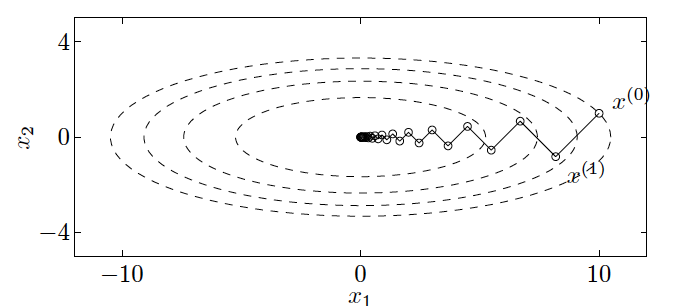
\includegraphics[width=0.8\textwidth]{\imgpath/sgd_bounce.png}
  \mycaption{Trajectory of gradient descent in an ellipsoidal parabola}{Some contour lines of
  the function $f(x)=1/2\left(x_1^2 + 10x_2^2 \right)$ and the trajectory of GD
  optimization using exact line search.
  This space has condition number 10, and shows the slow convergence of GD in
  spaces with largely different eigenvalues.
  Image taken from \cite{boyd_convex_2004} Figure 9.2.}
  \label{fig:ch2:gd_bounce}
\end{figure}

\subsection{Stochastic Gradient Descent}
Aside from the problems associated the curvature of the function $J(\theta)$,
another common issue faced with the gradient descent of \eqref{eq:ch2:gd} is the
cost of computing $\dydx{J}{\theta}$. In particular, the first term:
\begin{eqnarray}\label{eq:ch2:ldata}
  L_{data}(y, f(x, \theta)) &=& \mathbb{E}_{x,y \sim p_{data}}\left[ L_{data}(y, f(x, \theta))\right] \\
&=& \frac{1}{N}\sum_{n=1}^N L_{data}\left(y^{(n)}, f(x^{(n)}, \theta)\right) 
\end{eqnarray}
involves evaluating the entire dataset at the current values of $\theta$. As the
training set size grows into the thousands or millions of examples, this
approach becomes prohibitively slow. 

\eqref{eq:ch2:ldata} writes the data loss as an expectation, hinting at the fact that 
we can remedy this problem by using fewer samples $N_b < N$ to evaluate $L_{data}$. 
This variation is called Stochastic Gradient Descent (SGD).

Choosing the batch size is a hyperparameter choice that we must think carefully
about. Setting the value very low, e.g. $N_b = 1$ can be advantageous as the
noisy estimates for the gradient have a regularizing effect on the network
\cite{wilson_general_2003}. Increasing the batch size to larger values allows
you to easily parallelize computation as well as increasing your accuracy for
the gradient, allowing you to take larger step sizes \cite{smith_dont_2017}.
A good initial starting point is to set the batch size to about 100 samples and
increase/decrease from there \cite{goodfellow_deep_2016}.

\subsection{Gradient Descent and Learning Rate}
The step size parameter, $\eta$ in \eqref{eq:ch2:gd} is commonly referred to as
the learning rate. Choosing the right value for the learning rate is key.
Unfortunately, the line search algorithm in \eqref{eq:ch2:search} would be too
expensive to compute for neural networks (as would involve evaluating the
function several times at different values), each of which takes about as long
as calculating the gradients themselves. Additionally, as the gradients are
typically estimated over a mini-batch and are hence noisy there may be
little added benefit in optimizing the step sizes in the estimated direction. 

\autoref{fig:ch2:sgd_lr} illustrates the effect the learning rate can have over
a contrived convex example. Optimizing over more complex loss surfaces only
exacerbates the problem. Sadly, choosing the initial learning rate is 
`more of an art than a science' \cite{goodfellow_deep_2016}, but
\cite{bottou_stochastic_2012, montavon_neural_2012} have some tips on what to
set this at. We have found in our work that searching for a large learning 
rate that causes the network to diverge and reducing it hence can be a good
search strategy. This agrees with Section 1.5 of \cite{lecun_efficient_2012}
which states that for regions of the loss space which are roughly quadratic,
$\eta_{max} = 2\eta_{opt}$ and any learning rate above $2\eta_{opt}$ causes
divergence.

On top of the initial learning rate, the convergence of SGD methods require:
\begin{eqnarray}
  \sum_{t=1}^{\infty} \eta_t &\rightarrow &\infty \\
  \sum_{t=1}^{\infty} \eta_t^2 &=& M
\end{eqnarray}
where $M$ is finite. Choosing how to do this also contains a good amount of artistry,
and there is no one scheme that works best. A commonly used greedy method is to
keep the learning rate constant until the training loss stabilizes and then to
enter the next phase of training by setting $\eta_{k+1} = \gamma \eta_{k}$ where
$\gamma$ is a decay factor. Choosing $\gamma$ and the thresholds for triggering
a step however must be chosen by monitoring the training loss curve and trial
and error.

\begin{figure}[t]
  \centering
  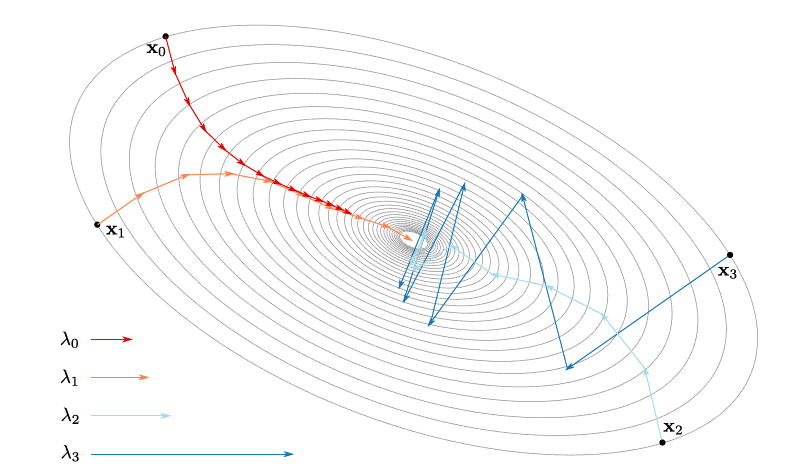
\includegraphics[width=\textwidth]{\imgpath/sgd_lr.png}
  \mycaption{Trajectories of SGD with different initial learning rates}{This
  figure illustrates the effect the step size has over the optimization process
  by showing the trajectory for $\eta = \lambda_i$ from equivalent starting
  points on a symmetric loss surface. Increasing the step size beyond
  $\lambda_3$ can cause the optimization procedure to diverge. Image
  taken from \cite{Ioannou2017thesis} Figure 2.7.}
  \label{fig:ch2:sgd_lr}
\end{figure}

\subsection{Momentum and Adam}
One simple and very popular modification to SGD is to add \emph{momentum}.
Momentum accumulates past gradients with an exponentially moving average and
continues to move in their direction. The name comes from the analogy of finding
a minimum of a function to rolling a ball over a loss surface --
any new force (newly computed gradients) must overcome the past motion of the
ball. To do this, we create a \emph{velocity} variable $v_{t}$ and modify
\eqref{eq:ch2:gd} to be:
\begin{eqnarray}
  v_{t+1} &=& \alpha v_t - \eta_k\dydx{J}{\theta} \label{eq:ch2:velocity}\\
  \theta_{t+1} &=& \theta_t + v_{t+1} \\
\end{eqnarray}
where $0\leq\alpha<1$ is the momentum term indicating how quickly to `forget'
past gradients.

Another popular modification to SGD is the adaptive learning rate technique Adam
\cite{kingma_adam:_2014}. There are several other adaptive schemes such as
AdaGrad \cite{duchi_adaptive_2011} and AdaDelta \cite{zeiler_adadelta:_2012}, but
they are all quite similar, and Adam is often considered the most robust of the
three \cite{goodfellow_deep_2016}. The goal of all of these adaptive schemes is
to take larger update steps in directions of low variance, helping to minimize
the effect of large condition numbers we saw in \autoref{fig:ch2:sgd_bounce}.
Adam does this by keeping track of the first $m_t$ and second $v_t$ moments of the
gradients:
\begin{eqnarray}
  g_{t+1} &=& \dydx{J}{\theta} \\
  m_{t+1} &=& \beta_1 m_{t} + (1-\beta_1)g_{t+1} \label{eq:ch2:adam_first}\\
  v_{t+1} &=& \beta_2 m_{t} + (1-\beta_2)g_{t+1} \\
\end{eqnarray}
where $0 \leq \beta_1, \beta_2 < 1$. Note the similarity between updating the
mean estimate in \eqref{eq:ch2:adam_first} and the velocity term in
\eqref{eq:ch2:velocity}\footnote{The $m_{t+1}$ and $v_{t+1}$ terms are then
bias-corrected as they are biased towards zero at the beginning of training. We
do not include this for conciseness.}. The parameters are then updated with:
\begin{equation}
  \theta_{t+1} = \theta_t - \eta \frac{m_{t+1}}{\sqrt{v_{t+1}} + \epsilon}
\end{equation}
where $\epsilon$ is a small value to avoid dividing by zero. 

\section{Neural Networks}\label{sec:cnns}

\subsection{The Neuron and Single Layer Neural Networks}

The neuron, shown in \autoref{fig:singlelayer} is the core building block of
Neural Networks. It takes the dot product between an  input vector $\vec{x} \in
\reals[N]$ and a weight vector $\vec{b}$, before applying a chosen nonlinearity,
$f$. I.e.

$$y = f(\langle\vec{x}, \vec{w}\rangle) = f\left(\sum_{i=0}^{N} x_i w_i \right) $$

where we have used the shorthand $b=w_0$ and $x_0 = 1$. 
Note that if $\langle\vec{w}, \vec{w}\rangle = 1$ then $\langle\vec{x},
\vec{w}\rangle$ is the distance from the point $\vec{x}$ to the hyperplane with
normal $\vec{w}$. With general $\vec{w}$ this can be thought of as a scaled
distance.  

Typical nonlinear functions $f$ are the sigmoid function: (\textbf{include figure})

$$\sigma(x) = \frac{1}{1+e^{-x}}$$

tanh function:

$$\F{tanh}(x) = \frac{e^{x} - e^{-x}}{e^{x} + e^{-x}}$$

or ReLU:

$$\F{ReLU}(x) = \max (x, 0)$$

The weight vector $\vec{w}$ defines a hyperplane in $\reals[N]$ which splits the
space into two. The choice of nonlinearity then affects how points on each side
of the plane are treated. For a sigmoid, points far below the plane get mapped
to 0 and points far above the plane get mapped to 1 (with points near the plane
having a value of 0.5). For tanh nonlinearities, these points get mapped to -1
and 1. For ReLU nonlinearities, every point below the plane ($\langle\vec{x},
\vec{w}\rangle < 0$) gets mapped to zero and every point above the plane keeps
its inner product value.

\begin{figure}
  \centering
  \pagestyle{empty}

\def\layersep{2.5cm}

\begin{tikzpicture}[shorten >=1pt,->,draw=black!50, node distance=\layersep]
    \tikzstyle{every pin edge}=[<-,shorten <=1pt]
    \tikzstyle{neuron}=[circle,draw=black,minimum size=17pt,inner sep=0pt]
    \tikzstyle{input neuron}=[neuron];
    \tikzstyle{output neuron}=[neuron, fill=red!50];
    \tikzstyle{hidden neuron}=[neuron];
    \tikzstyle{annot} = [text width=4em, text centered]

    % Draw the input layer nodes
    \foreach \name / \y in {0,...,4}
    % This is the same as writing \foreach \name / \y in {1/1,2/2,3/3,4/4}
        \node[input neuron,pin=left:$x_\y$] (I-\name) at (0,-\y) {};
    \node[input neuron,pin=left:1] (I-5) at (0,-5) {};

    % Draw the output layer node
    \node[hidden neuron,pin={[pin edge={->}]right:$y$}] (O) at (\layersep, -2.5) {};

    % Connect every node in the input layer with every node in the
    % hidden layer.
    % \foreach \source in {1,...,5}
        % \draw(I-\source) edge (O) node[above, midway] {$w_\source$};
    \foreach \source in {0,...,4}
        \draw[->] (I-\source) -- (O) node[above,midway] {$w_\source$};
    \draw[->] (I-5) -- (O) node[above,midway] {$b$};

    % Annotate the layers
    % \node[annot,above of=I-1, node distance=1cm] (il) {Input Layer};
    % \node[annot,right of=hl] {Output layer};
\end{tikzpicture}
% End of code
\label{fig:singlelayer}
  \mycaption{A single neuron}{The neuron is composed of inputs $x_i$, weights
    $w_i$ (and a bias term), as well as an activation function. Typical activation
    functions include the sigmoid function, tanh function and the ReLU}
\end{figure}

Consider a single neuron acting as logistic regressor. I.e.\ we have 
$\mathcal{D} = \{\vec{x}_i, y_i\}$ where $y_i \in \{0, 1\}$. 
We can easily find the maximum likelihood estimates for $\vec{w}$ by minimizing
the loss

\subsection{Loss or Error Term}

\subsection{Backpropagation}

With a deep network like most CNNs, calculating $\dydx{L}{w}$ may not seem
particularly obvious if $w$ is a weight in one of the lower layers.  Say we have
a deep network, with $L$ layers. We need to define a rule for updating the
weights in all $L$ layers of the network, however, only the weights $w_L$ are
connected to the loss function, $\loss$. We assume for whatever function the
last layer is that we can write down the derivative of the output with respect
to the weights $\dydx{z_{L}}{w_{L}}$. We can then write down the weight-update
gradient, $\dydx{\loss}{w_L}$ with application of the chain rule:

\begin{equation}
  \dydx{\loss}{w_L} = \dydx{\loss}{z_L} \dydx{z_L}{w_L} + \underbrace{\lambda
  w}_{\text{from the reg.\ loss}}
\end{equation}

$\dydx{\loss}{z_L}$ can be done simply from the equation of the loss function
used. Typically this is parameterless.

Since all of the layers in a CNN are well-defined and
differentiable\footnote{The ReLU is not differentiable at its corner, but
backpropagation can still be done easily by simply looking at the sign of the
input.} we assume that we can also write down what $\dydx{z_L}{z_{L-1}}$ is.
Repeating this process for the next layer down, we have:

\begin{equation}
  \dydx{\loss}{w_{L-1}}
  = \dydx{\loss}{z_L}\dydx{z_L}{z_{L-1}}\dydx{z_{L-1}}{w_{L-1}}
\end{equation}

We can generalize this easily like so:

\begin{equation}
  \dydx{\loss}{w_{l}}
  = \dydx{\loss}{z_L} \underbrace{\prod_{i=L}^{l+1}
  \dydx{z_i}{z_{i-1}}}_{\text{product to $l$'s output}} 
  \dydx{z_{l}}{w_{l}}
\end{equation}

So far we have defined the loss function for a given data point $(x^{(i)},
y^{(i)})$. Typically, we want our network to be able to generalize to the true
real world joint distribution $P(x,y)$, minimizing the expected risk ($R_E$) of
loss:

\begin{equation}
  R_E(f(x,w)) = \int \loss(y,f(x,w)) dP(x,y)
\end{equation}

Instead, we are limited to the training set, so we must settle for the
empirical risk ($R_{EMP}$):

\begin{equation}
  R_{EMP}(f(x,w)) = \frac{1}{N} \sum_{i=1}^{N} \loss( y^{(i)},f(x^{(i)}, w))
  \label{eq:empirical_risk}
\end{equation}

\subsection{Gradient descent vs Stochastic Gradient Descent vs Mini-Batches}
  We can minimize \autoref{eq:empirical_risk} with \emph{gradient descent}
  \citep{rumelhart_parallel_1986}. Updates can be made on a generic network
  parameter $w$ with:
  \begin{equation}
    w_{t+1} = w_{t} - \eta \dydx{E_n}{w}
  \end{equation}
  where $\eta$ is caleld the learning rate. Calculating the gradient
  $\dydx{E_n}{w}$ is done by averaging the individual gradients
  $\dydx{\loss}{w}$ over the entire training dataset. This can be very slow,
  particularly for large training sets.
  
  Instead, we can learn far more quickly by using a single estimate for the
  weight update equation, i.e., 
  \begin{equation}
    w_{t+1} = w_{t} - \eta \dydx{\loss}{w}
  \end{equation}
  This is called \emph{stochastic gradient descent}. Each weight update now
  uses a noisy estimate of the true gradient $\dydx{E_n}{w}$. Carefully
  choosing the learning rate $\eta$ update scheme can ensure that the network
  converges to a local minimum, but the process may not be smooth (the
  empirical risk may fluctuate, which could be interpreted as the network
  diverging).

  An often used trade off between these two schemes is called \emph{mini-batch
  gradient descent}. Here, the variance of the estimate of $\dydx{E_n}{w}$ is
  reduced by averaging out the point estimate $\dydx{L}{w}$ over a mini-batch
  of samples, size $N_B$. Typically $1 << N_B << N$, with $N_B$ usually being
  around 128. This number gives a clue to another benefit that has seen the use
  of mini-batches become standard --- they can make use of parallel processing.
  Instead of having to wait until the gradient from the previous data point was
  calculated and the network weights are updated, a network can now process
  $N_B$ samples in parallel, calculating gradients for each point with the same
  weights, average all these gradients in one quick step, update the weights,
  and continue on with the next $N_B$ samples. The update equation is now:
  \begin{equation}
    w_{t+1} = w_{t} - \eta \sum_{n=1}^{N_B} \dydx{\loss}{w}
  \end{equation}

\subsubsection{Loss Functions}
  For a given sample $q=(x, y)$, the loss
  function is used to measure the cost of predicting $\hat{y}$ when the
  true label was $y$. We define a loss function $\loss (y, \hat{y})$. 
  A CNN is a deterministic
  function of its weights and inputs, $f(x,w)$ so this can be written as $\loss
  (y, f(x,w))$, or simply $\loss(y, x, w)$.
  
  It is important to remember that we can choose
  to penalize errors however we please, although for CNNs, the vast majority of
  networks use the same loss function --- the softmax loss. Some networks have
  experimented with using the hinge loss function (or `SVM loss'), stating they
  could achieve improved results \citep{gu_recent_2015,tang_deep_2013}. 
  \begin{enumerate}

  \item \emph{Softmax Loss:} The more common of the two, the softmax turns
    predictions into non-negative, unit summing values, giving the sense of
    outputting a probability distribution. The softmax function is applied to
    the $C$ outputs of the network (one for each class):
    \begin{equation}
      p_j = \frac{e^{(f(x, w))(j)}}{\sum\limits_{k=1}^{C}e^{(f(x,w))(k)}}
    \end{equation}
    where we have indexed the $c$-th element of the output vector $f(x,w)$ with
      $(f(x,w))(c)$. The softmax \emph{loss} is then defined as:
    \begin{equation}
      \loss (y_i, x, w)
      = \sum_{j=1}^{C} \mathbbm{1}\{y_i=j\} \log p_j
    \end{equation}
    Where $\mathbbm{1}$ is the indicator function, and $y_i$ is the true label
    for input $i$.

  \item \emph{Hinge Loss:} The same loss function from Support Vector
    Machines (SVMs) can be used to train a large margin classifier in a CNN:
    \begin{equation}
      \loss(y,x,w) = \sum_{l=1}^{C} 
        {\left[ \max(0, 1 - \delta(y_i,l) w^{T}x_{i}) \right]}^p \label{eq:nn_hinge_loss}
    \end{equation}
    Using a hinge loss like this introduces extra parameters, which would
    typically replace the final fully connected layer. The $p$ parameter in
    \autoref{eq:nn_hinge_loss} can be used to choose $\ell^1$ Hinge-Loss, or
    $\ell^2$ Squared Hinge-Loss. 

  \end{enumerate}
  

\subsubsection{Regularization}
  Weight regularization, such as an $\ell^2$ penalty is often given to the
  learned parameters of a system. This applies to the parameters of the fully
  connected, as well as the convolutional layers in a CNN\@. These are added to
  the loss function. Often the two loss components are differentiated between by
  their monikers - `data loss' and `regularization loss'. The above 
  equation then becomes:
  \begin{equation}
    \mathcal{L} = \mathcal{L}_{data} + \underbrace{\frac{1}{2}\lambda_{fc}
    \sum_{i=1}^{L_{fc}} \sum_{j} \sum_{k} {(w_{i}[j,k])}^2}_{\text{fully connected
    loss}} +
    \underbrace{\frac{1}{2}\lambda_{c} \sum_{i=1}^{L_c} \sum_{u_1} \sum_{u_2} \sum_{d}
    \sum_{n} \left(f_i[u_1,u_2,d,n]\right)^2}_{\text{convolutional loss}}
  \end{equation}

  Where $\lambda_{fc}$ and $\lambda_{c}$ control the regularization parameters
  for the network. These are often also called `weight decay' parameters.

  The choice to split the $\lambda$'s between fully connected and convolutional
  layers was relatively arbitrary. More advanced networks can make $\lambda$
  a function of the layer. 


\subsection{Learning}

\subsection{Optimization}

\subsection{Extending to multiple layers and different block types}
\begin{figure}
  \centering
  \begin{tikzpicture}[every node/.style={node font=\large}]
\definecolor{mycolor}{RGB}{252,247,189};
\pgfmathsetmacro{\EDGE}{.5}
\node [fill=mycolor, draw, minimum width=3cm, minimum height=2cm] (block) at (1,1) {$y=f(x,w)$};
\coordinate[right=\EDGE of block.south west] (xin);
\coordinate[left=\EDGE of block.south east] (dxin);
\coordinate[below=\EDGE of block.north west] (win);
\coordinate[above=\EDGE of block.south west] (dwin);
\coordinate[right=\EDGE of block.north west] (yin);
\coordinate[left=\EDGE of block.north east] (dyin);
\draw[<-] (xin) -- +(0,-1) node[below] {$x$};
\draw[->] (dxin) -- ++(0,-1) node[below] {$\dydx{\logloss}{x}$};
\draw[<-] (win) -- ++(-1,0) node[left] {$w$};
\draw[->] (dwin) -- ++(-1,0) node[left] {$\dydx{\logloss}{w}$};
\draw[->] (yin) -- ++(0,1) node[above] {$y$};
\draw[<-] (dyin) -- ++(0,1) node[above] {$\dydx{\logloss}{y}$};
\end{tikzpicture}

\end{figure}

\subsubsection{Convolutional Layers}
  The image/layer of features is convolved by a set of filters.
  The filters are typically small, ranging from $3\x 3$ in ResNet and VGG
  to $11\x 11$ in AlexNet. We have quoted only spatial size
  here, as the filters in a CNN are always \emph{fully connected in depth} ---
  i.e.,\ they will match the number of channels their input has.

  For an input $\bmu{x} \in \mathbb{R}^{H\x W\x D}$, and filters 
  $\bmu{f} \in \mathbb{R}^{H'\x W'  \x D \x D''}$ ($D''$ is the 
  number of filters), our output $\bmu{z} \in
  \mathbb{R}^{H''\x W'' \x D''}$ will be given by:
  \begin{equation}
    z[u_1, u_2, d''] = b[d''] + \sum_{i=-\frac{H'}{2}}^{\frac{H'}{2}-1}
                       \sum_{j=-\frac{W'}{2}}^{\frac{W'}{2}-1}  \sum_{k=0}^{D-1}  
                        f[i, j, k, d''] x[u_1-i, u_2-j, k]
  \end{equation}

\subsubsection{ReLUs}
  Activation functions, neurons, or non-linearities, are the core of a neural networks
  expressibility. Historically, they were sigmoid or tanh functions, but these
  have been replaced recently by the Rectified Linear Unit (ReLU), which has
  equation $g(x) = \max(0,x)$. A ReLU
  non-linearity has two main advantages over its smoother predecessors~\citep{%
  glorot_deep_2011, nair_rectified_2010}.
  \begin{enumerate}
  \item It is less sensitive to initial conditions as the gradients that
    backpropagate through it will be large even if $x$ is large. A common
    observation of sigmoid and tanh non-linearities was that their learning would
    be slow for quite some time until the neurons came out of saturation, and then
    their accuracy would increase rapidly before levelling out again at
    a minimum~\citep{glorot_understanding_2010}. The ReLU, on the other hand, has
    constant gradient.
  \item It promotes sparsity in outputs, by setting them to a hard 0. Studies
    on brain energy expenditure suggest that neurons encode information in
    a sparse manner. \citet{lennie_cost_2003} estimates the percentage of
    neurons active at the same time to be between 1 and 4\%. Sigmoid and tanh
    functions will typically have \emph{all} neurons firing, while 
    the ReLU can allow neurons to fully turn off.
  \end{enumerate}

  \begin{figure}
    \centering
      % \section{Wavelet-Based Nonlinearities}\label{sec:ch6:nonlinearities}
Returning to the goals from \autoref{sec:ch6:learning}, the experiments from the
previous section have shown that while it is possible to use a wavelet gain
layer ($G$) in place of a convolutional layer ($H$), this may come with a small
performance penalty. Ignoring this effect for the moment, in this section, we
continue with our investigations into learning in the wavelet domain. In
particular, is it possible to replace a pixel domain nonlinearity $\sigma$ with
a wavelet-based one $\sigma_w$?

But what sensible nonlinearity should be used? Two particular options are good initial
candidates:
\begin{enumerate}
  \item The ReLU: this is a mainstay of most modern neural networks and has
    proved invaluable in the pixel domain. Its pseudo-nonlinearity
    ($\F{ReLU}(Ax) = A\F{ReLU}(x)$) makes learning less dependent on signal
    amplitudes. Perhaps its sparsifying
    properties will work well on wavelet coefficients too. 
  \item Thresholding: a technique commonly applied to wavelet
    coefficients for denoising and compression. Many proponents of compressed
    sensing and dictionary learning even like to compare soft thresholding to a
    two-sided ReLU \cite{papyan_theoretical_2018, papyan_convolutional_2017-1}.
\end{enumerate}

In this section, we will look at both and see if they improve the gain
layer. If they do, it would the be possible to connect multiple layers in the
wavelet domain, avoiding the necessity to do inverse wavelet transforms after
learning.

\subsection{ReLUs in the Wavelet Domain}
Applying the ReLU to the real lowpass coefficients is not difficult, but it does
not generalize so easily to complex coefficients. The simplest option is to apply
it independently to the real and imaginary coefficients, effectively only
selecting one quadrant of the complex plane:
\begin{align}
  u_{lp} &= \F{max}(0,\ v_{lp}) \\
  u_{j} &= \F{max}(0,\ \real{v_{j}}) + j\F{max}(0,\ \imag{v_j}) \label{eq:ch6:relu_bp}
\end{align}

Another option is to apply it to the magnitude of the bandpass coefficients. Of
course, these are all strictly positive so the ReLU on its own would not do
anything. However, they can be arbitrarily scaled and shifted by using a batch
normalization layer. Then the magnitude could shift to (invalid) negative
values, which can then be rectified by the ReLU.

Dropping the scale subscript $j$ for clarity (we need it for the square root of 
negative 1), let a bandpass coefficient at a given scale be
$v = r_v e^{j\theta_v}$ and define
$\mu_r = \mathbb{E}[r_v]$ and $\sigma_r^2 = \mathbb{E}[(r_v-\mu_r)^2]$, then
applying batch-normalization and the ReLU to the magnitude of $v_j$ means we
get:
\begin{align}
  r_u &= \F{ReLU}(BN(r_v)) = \max(0,\ \gamma \frac{r_v-\mu_r}{\sigma_r} + \beta) \label{eq:ch6:magrelu_bp} \\
  u &= r_u e^{j\theta_v} \label{eq:ch6:magrelu_bp2}
\end{align}
This also works equivalently on the lowpass coefficients, although $v_{lp}$ can
be negative unlike $r_v$:
\begin{equation}
  u_{lp} = \F{ReLU}(BN(v_{lp})) = \max(0, \gamma' \frac{v_{lp} - \mu_{lp}}{\sigma_{lp}} + \beta') \label{eq:ch6:bnrelu_lp}
\end{equation}
%
\subsection{Thresholding}
For $t \in \reals$ and $z = re^{j\theta} \in \complexes$ the pointwise hard thresholding is:
\begin{align}
  \mathcal{H}(z, t) &= \left\{ \begin{array}{ll}
    z & r \geq t \\
    0 & r < t\\
  \end{array} \right. \\
  &= \indic(r > t) z
\end{align}
and the pointwise soft thresholding is:
\begin{align}
  \mathcal{S}(z, t) &= \left\{ \begin{array}{ll}
    (r-t)e^{j\theta} & r \geq t \\
    0 & r < t\\
  \end{array} \right. \\
  &= \max(0, r - t)e^{j\theta} \label{eq:ch6:relu_st}
\end{align}
Note that \eqref{eq:ch6:relu_st} is very similar to \eqref{eq:ch6:magrelu_bp} and \eqref{eq:ch6:magrelu_bp2}.
We can rewrite \eqref{eq:ch6:magrelu_bp} by taking the strictly positive terms
$\gamma$, $\sigma$ outside of the $\max$ operator:
\begin{align}
  r_u &= \max(0, \gamma \frac{r_v-\mu_r}{\sigma_r} + \beta) \\
      &= \frac{\gamma}{\sigma_r}\max\left(0, r_v - \left(\mu_r - \frac{\sigma_r\beta}{\gamma}\right)\right) \label{eq:ch6:bnrelu_soft}
\end{align}
then if $t' = \mu_v - \frac{\sigma_r\beta}{\gamma} > 0$, \textbf{doing batch
normalization followed by a ReLU on the magnitude of the complex coefficients is the
same as soft shrinkage with threshold $t'$, scaled by a factor
$\frac{\gamma}{\sigma_r}$}.

The same analogy does not apply to the lowpass
coefficients, as $v_{lp}$ is not strictly positive.

While soft thresholding is similar to batch normalizations and ReLUs, we would also like
to test how well it performs as a sparsity-inducing wavelet nonlinearity.
To do this, we can:
\begin{itemize}
  \item Learn the threshold $t$
  \item Adapt $t$ as a function of the distribution of activations to achieve a desired sparsity level.
\end{itemize}
In early experiments, we found that trying to set
desired sparsity levels by tracking the standard deviation of the statistics
and setting a threshold as a function of it performed very poorly (causing a
drop in top-1 accuracy of at least 10\%).
Instead, we choose to learn a threshold $t$. We make this an unconstrained
optimization problem by changing \eqref{eq:ch6:relu_st} to:
\begin{equation}
  \mathcal{S}(v, t) = \max(0, r-|t|)e^{j\theta}  \label{eq:ch6:relu_st2}
\end{equation}

Learning a threshold is only possible for soft thresholding, as $\dydx{L}{t}$ is
not defined for hard thresholding. Like batch normalization, we learn
independent thresholds $t$ for each channel.

      \caption[Differences in non-linearities]
              {Differences in non-linearities. Green --- the \emph{sigmoid} function, 
               Blue --- the \emph{tanh} function, and Red --- the \emph{ReLU}. The ReLU
               solves the problem of small gradients outside of the activation
               region (around $x=0$) as well as promoting sparsity.}\label{fig:nonlinearities}
  \end{figure}


\subsubsection{Pooling}
  Typically following a convolutional layer (but not strictly), activations are subsampled with
  max pooling. Pooling adds some invariance to shifts smaller than the pooling
  size at the cost of information loss. For this reason, small pooling is
  typically done often $2\x 2$ or $3\x 3$, and the invariance to larger shifts
  comes after multiple pooling (and convolutional) layers.
  
  While initial designs of max pooling would do it in non-overlapping regions, 
  AlexNet used $3\x 3$ pooling with stride 2 in their breakthrough design,
  quoting that it gave them an increase in accuracy of roughly $0.5\%$ and
  helped prevent their network from `overfitting'. More recent networks will
  typically employ either this or the original $2\x 2$ pooling with stride 2,
  see \autoref{fig:maxpool}. A review of pooling methods in
  \citep{mishkin_systematic_2016} found them both to perform equally well.
  
  \begin{figure}
    \centering
    % \subfloat[]{%
        % \input{tikz/maxpool.tex}\label{fig:maxpool_tight}
    % }
%    \newline
    \centering
    % \subfloat[]{%
        % \input{tikz/maxpool_overlap.tex}\label{fig:maxpool_overlap}
    % }
    \caption[Tight vs.\ overlapping pooling]
            {\subref{fig:maxpool_tight} Tight $2\x 2$ pooling with stride 2, vs
            \subref{fig:maxpool_overlap} overlapping $3\x 3$ pooling with
            stride 2. Overlapping pooling has the possibility of having one
            large activation copied to two positions in the reduced size
            feature map, which places more emphasis on the odd columns.}
    \label{fig:maxpool}
  \end{figure}

\subsubsection{Batch Normalization}
      Batch normalization proposed only very recently in
      \citep{ioffe_batch_2015} is a conceptually simpler technique. Despite
      that, it has become quite popular and has been found to be very useful.
      At its core, it is doing what standard normalization is doing, but also
      introduces two learnable parameters --- scale ($\gamma$) and offset
      ($\beta$).
      \autoref{eq:normalization} becomes:
      \begin{equation}
        \tilde{z}(u_1,u_2,d) = \gamma\frac{z-E[z]}{\sqrt{Var[z]}} + \beta 
				\label{eq:batch_normalization}
      \end{equation}
      These added parameters make it a \emph{renormalization} scheme, as instead of
      centring the data around zero with unit variance, it can be centred
      around an arbitrary value with arbitrary variance. S etting
      $\gamma = \sqrt{Var[z]}$ and $\beta = E[z]$, we would get the identity
      transform. Alternatively, setting $\gamma = 1$ and $\beta = 0$ (the
      initial conditions for these learnable parameters), we get standard
      normalization.
      
      The parameters $\gamma$ and $\beta$ are learned through backpropagation.
      As data are usually processed in batches, the gradients for $\gamma$ and
      $\beta$ are calculated per sample, and then averaged over the whole
      batch.

      From \autoref{eq:batch_normalization}, let us briefly use the hat
      notation to represent the standard normalized input:
      $\hat{z} = (z-E[z])/\sqrt{Var[z]}$, then:
      \begin{eqnarray}
        \tilde{z}^{(i)} & = & \gamma \hat{z}^{(i)} + \beta \nonumber\\
        \frac{\partial \mathcal{L}}{\partial \gamma}& =&
        \frac{1}{N}\sum_{i=1}^{N} \frac{\partial
        \mathcal{L}^{(i)}}{\partial \tilde{z}^{(i)}} \cdot \hat{z}^{(i)} \\
        \frac{\partial \mathcal{L}}{\partial \beta}& =&
        \frac{1}{N}\sum_{i=1}^{N} \frac{\partial
        \mathcal{L}^{(i)}}{\partial \tilde{z}^{(i)}} 
      \end{eqnarray}

      Batch normalization layers are typically placed \emph{between} convolutional layers
      and non-linearities. I.e.,\ if $Wu+b$ is the output of a convolutional
      layer, and $z=g(Wu+b)$ is the output of the non-linearity, then with the
      batch normalization step, we have:
      \begin{eqnarray}
        z &=& g(BN(Wu+b)) \nonumber\\
          &=& g(BN(Wu))
      \end{eqnarray}
      Where the bias term was ignored in the convolutional layer, as it can be
      fully merged with the `offset' parameter $\beta$.

      This has particular benefit of removing the sensitivity of our network to
      our initial weight scale, as for scalar $a$,
      \begin{equation}
        BN(Wu) = BN((aW)u)
      \end{equation}
      It is also particularly useful for backpropagation, as an increase in
      weights leads to \emph{smaller} gradients \citep{ioffe_batch_2015}, making
      the network far more resilient to the problems of vanishing and exploding
      gradients:
      \begin{eqnarray}
        \frac{\partial BN((aW)u)}{\partial u} & = & \frac{\partial
        BN(Wu)}{\partial u} \nonumber\\
        \frac{\partial BN((aW)u)}{\partial (aW)} & = & \frac{1}{a} \cdot \frac{\partial
        BN(Wu)}{\partial W} 
      \end{eqnarray}


\section{Relevant Architectures}

\subsection{LeNet}
\subsection{AlexNet}
\subsection{VGG}
\subsection{Residual Networks}
  The current state of the art design introduced a clever novel feature called
  a residual unit\citep{he_deep_2015,he_identity_2016}. The inspiration for their design came from the difficulties
  experienced in training deeper networks. Often, adding an extra layer would
  \emph{decrease} network performance. This is counter-intuitive as the deeper
  layers could simply learn the identity mapping, and achieve the same
  performance.

  To promote the chance of learning the identity mapping, they define
  a residual unit, shown in \autoref{fig:residual_unit}. If a desired mapping
  is denoted $\mathcal{H}(x)$, instead of trying to learn this, they instead
  learn $\mathcal{F}(x) = \mathcal{H}(x) - x$. 
  \begin{figure}
    \centering
    % 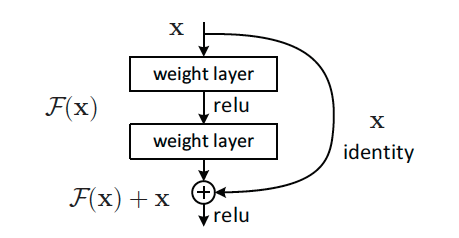
\includegraphics[width=0.5\textwidth]{images/residual_unit.png}
    \caption[The residual unit from ResNet]
          {A residual unit. The identity mapping is always present, and the
            network learns the difference from the identity mapping, $\mathcal{F}(x)$.
            Taken from \citep{he_deep_2015}.}
      \label{fig:residual_unit}
  \end{figure}


\subsection{old}
  Convolutional Neural Networks (CNNs) were initially introduced by \citet{lecun_backpropagation_1989} in
  \citep{lecun_backpropagation_1989}. Due to the difficulty of training and
  initializing them, they failed to be popular for more than two decades.  This
  changed in 2012, when advancements in pre-training with unsupervised networks
  \citep{bengio_greedy_2007}, the use of an improved non-linearity --- the Rectified Linear
  Unit, or ReLU, new regularization methods\citep{hinton_improving_2012}, and
  access to more powerful computers in graphics cards, or GPUs, allowed
  Krizhevsky, Sutskever and Hinton  to develop
  AlexNet\citep{krizhevsky_imagenet_2012}. This network nearly halved the
  previous state of the art's error rate.  Since then, interest in them has
  expanded very rapidly, and they have been successfully applied to object
  detection~\citep{ren_object_2015} and human pose estimation
  \citep{tompson_efficient_2015}. It would take a considerable amount of effort
  to document the details of all the current enhancements and tricks many
  researches are using to squeeze extra accuracy, so for the purposes of this
  report we restrict ourselves to their generic design, with some time spent
  describing some of the more promising enhancements. 
  
  We would like to make note of some of the key architectures
  in the history of CNNs, which we, unfortunately, do not have space to describe:
  \begin{itemize}
    \item Yann LeCun's LeNet-5~\citep{lecun_gradient-based_1998}, the state of the art
      design for postal digit recognition on the MNIST dataset.
    \item Google's GoogLeNet~\citep{szegedy_going_2015} achieved $6.67\%$ top-5
      error on ILSVRC2014, introducing the new `inception' architecture, which
      uses combinations of $1\x 1$, $3\x 3$ and $5\x 5$ convolutions.
    \item Oxford's VGG~\citep{simonyan_very_2014} --- $6.8\%$ and runner up in
      ILSVRC2014. The VGG design is very similar to AlexNet but was roughly
      twice as deep. More convolutional layers were used, but with smaller
      support --- only $3\x 3$. These were often stacked directly on top of
      each other without a non-linearity in between, to give the effective
      support of a $5\x 5$ filter.
    \item Microsoft Research's ResNet~\citep{he_deep_2015} achieved $4.5\%$ top-5 
      error and was the winner of ILSVRC2015. This network we will talk briefly
      about, as it introduced a very nice novel layer --- the residual layer.
  \end{itemize}

  Despite the many variations of CNN architectures currently being used, most
  follow roughly the same recipe (shown in \autoref{fig:cnn_generic}):
  \begin{figure}
    \centering
      % 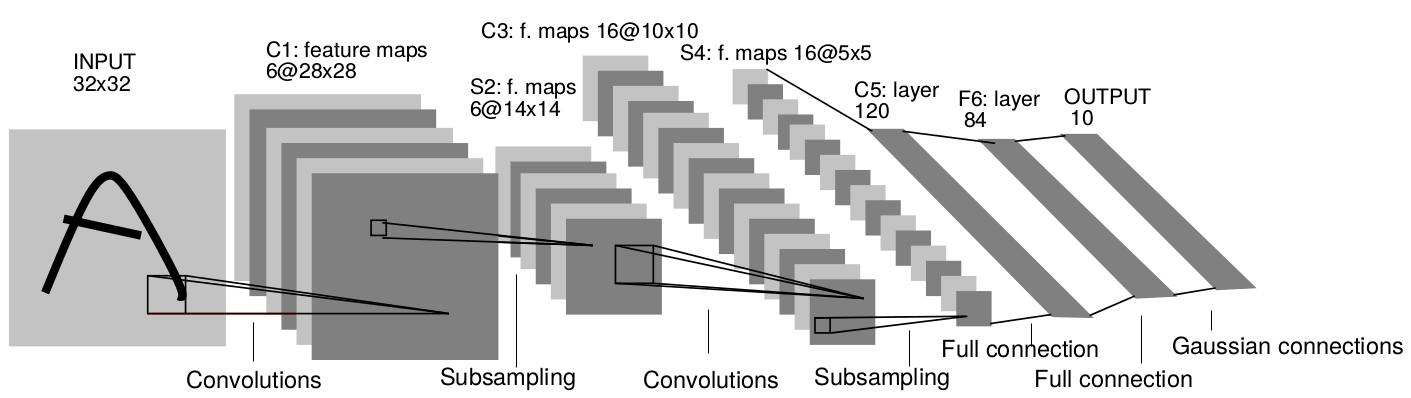
\includegraphics[width=\textwidth]{images/cnns.png}
      \caption[Standard CNN architecture]
              {Standard CNN architecture. Taken
              from~\citep{lecun_gradient-based_1998}}\label{fig:cnn_generic}
  \end{figure}

\subsection{Fully Connected Layers}\label{sec:cnn_fullyconnected}
  The convolution, pooling, and activation layers all
  conceptually form part of the \emph{feature extraction} stage of a CNN. One
  or more fully connected layers are usually placed after these layers to form
  the \emph{classifier}. One of the most elegant and indeed most powerful
  features of CNNs is this seamless connection between the \emph{feature
  extraction} and \emph{classifier} sub-networks, allowing the backpropagation
  of gradients through all layers of the entire network.

  The fully connected layers in a CNN are the same as those in a classical
  Neural Network (NN), in that they compute a dot product between their input
  vector and a weight vector:
  \begin{equation}
    z_i = \sum_{j} W_{ij}x_j
  \end{equation}
  The final output of the Fully Connected layer typically has the same number
  of outputs as the number of classes $C$ in the classification problem.


\section{The Fourier and Wavelet Transforms}

  Computer vision is an extremely difficult task. Pixel intensities in an image are
  typically not very informative in understanding what is in that image. Indeed,
  these values are sensitive to lighting conditions and camera configurations.
  It would be easy to take two photos of the same scene and get two vectors
  $x_1$ and $x_2$ that have a very large Euclidean distance, but to a human,
  would represent the same objects. What is most important in defining an image is
  difficult to define, however some things are notably more important than
  others. In particular, the location or phase of the waves that make up an
  image is much more important than the magnitude of these waves, something
  that is not necessarily true for audio processing. A simple experiment to
  demonstrate this is shown in \autoref{fig:ch2:barbara_morph}. 
  \begin{figure}
    \centering
      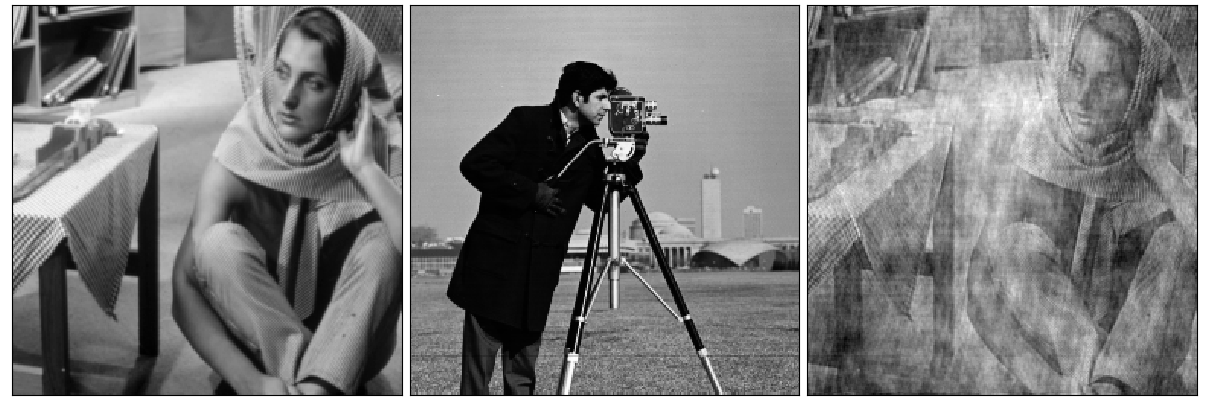
\includegraphics[width=\textwidth]{\imgpath/barbara_mag_swap.png}
      \mycaption{Importance of phase over magnitude for images}
        {The phase of the Fourier transform of the first image is combined with
        the magnitude of the Fourier transform of the second image and
        reconstructed. Note that the first image has entirely won out and
        nothing is left visible of the cameraman.}
      \label{fig:ch2:barbara_morph}
  \end{figure}

\subsection{The Fourier Transform}
For a signal $f(t) \in L_2(\reals)$ (square summable signals), the \emph{Fourier
transform} is defined as:
\begin{equation}
  F(\omega) = \int_{-\infty}^{\infty} f(t) e^{-j\omega t} dt
\end{equation}
This can be extended to two dimensions for signals $f(\xy) \in L_2(\reals[2])$:
\begin{equation}
  F(\ww) = \int_{-\infty}^{\infty}\int_{-\infty}^{\infty} f(\xy) e^{-j\ww^t \xy} d\xy = \langle f(\xy),\ e^{j\ww^t \xy} \rangle
\end{equation}

The Fourier transform is an invaluable signal expansion, as viewing a signal in
the frequency space offers many insights, as well as affording many very useful
properties (most notably the efficiency of convolution as a product of Fourier
transforms). While it is a mainstay in signal processing, 
it can be a poor
feature descriptor due to the infinite support of its basis functions - the
complex sinusoids $e^{j\ww^t u}$. If
a single pixel changes in the input it can change all of the
Fourier coefficients. As natural images are generally non-stationary, we need
to be able to isolate frequency components in local regions of an image, and
not have this property of global dependence. To achieve a more local Fourier
transform we can use the short time (or short space) Fourier Transform (STFT) or the
continuous wavelet transform (CWT). The two are very similar and mainly differ in the
way they handle the concept of `scale'. We will only discuss the CWT in this review, 
but for an excellent comparison of the two, we recommend \cite[Chapter~1]{antoine_two-dimensional_2004}.

% The Fourier transform does have one nice property, however, in that the magnitude of
% Fourier coefficients are invariant to global translations, a nuisance
% variability. We explore this theme more in our review of the Scattering
% Transform by \Mallat in \autoref{ch:scatternets}.

\subsection{The Continuous Wavelet Transform}
The \emph{continuous wavelet transform}, like the Fourier Transform, can be used
to decompose a signal into its frequency components. Unlike the Fourier
transform, these frequency components can be localized in space. To
achieve this, we need a bandpass filter, or \emph{mother wavelet}
$\psitd$\footnote{We use upright $\psiod, \phiod$ to distinguish 1-D wavelets
from their 2-D counterparts $\psitd, \phitd$} such that:
\begin{equation}
  \int_{-\infty}^{\infty} \psitd(\xy) d\xy = \Psi(0) = 0\label{eq:ch2:admissibility}
\end{equation}
Any function that has sufficient decay of energy with frequency and satisfies
\eqref{eq:ch2:admissibility}, is said to satisfy the \emph{admissibility condition}.

As we are working in 2-D for image processing, consider rotations, dilations, and 
shifts of this function by $\theta\in [0,2\pi],\ a>0,\ \bmu{b} \in \reals[2]$ respectively, where 
\begin{align}
  \text{Rotation: } & R_{\theta}x(\xy) = x(r_{-\theta}\xy) \label{eq:ch2:rot}\\
  \text{Dilation: } & D_{a}x(\xy) = \frac{1}{a} x\left(\frac{\xy}{a}\right), \quad a>0 \label{eq:ch2:di}\\
  \text{Translation: } & T_{\bmu{b}}x(\xy) = x(\xy - \bmu{b}) \label{eq:ch2:tr} 
\end{align}
where $r_\theta$ is the 2-D rotation matrix. Now consider shifts, scales and
rotations of our bandpass filter 
\begin{equation}
  \psitd_{\bmu{b},a, \theta}(\xy) = \frac{1}{a}\psitd \left(\frac{r_{-\theta}\left(\xy -
  \bmu{b}\right)}{a} \right) \label{eq:ch2:2d_shifts}
\end{equation}
which are called the \emph{daughter wavelets}. The 2D CWT of a signal $x(\xy)$ is defined as
\begin{equation}
  CWT_x(\bmu{b}, a, \theta) = \int_{-\infty}^{\infty} \psitd^*_{\bmu{b}, a,
  \theta}(\xy) x(\xy) d\xy = \langle \psitd_{\bmu{b}, a, \theta}(\xy),\ x(\xy)
  \rangle \label{eq:ch2:cwt}
\end{equation}

\subsubsection{Properties} 
The CWT has some particularly nice properties. In particular, it has \emph{covariance} 
under the three transformations \eqref{eq:ch2:tr}-\eqref{eq:ch2:rot}:
\begin{align}
  R_{\theta_0}x & \rightarrow CWT_x\left(r_{-\theta_0}\bmu{b}, a, \theta + \theta_0 \right)  \\
  D_{a_0}x & \rightarrow CWT_x\left(\bmu{b}/a_0, a/a_0, \theta \right) \\
  T_{\bmu{b}_0}x & \rightarrow CWT_x\left(\bmu{b}-\bmu{b}_0, a, \theta \right) 
\end{align}
Most importantly, the CWT is now localized in space, which distinguishes it from the
Fourier transform. This means that changes in one part of the image will not
affect the wavelet coefficients in another part of the image, so long as the
distance between the two parts is much larger than the support region of the
wavelets you are examining. 

\subsubsection{Inverse}
The CWT can be inverted by using a \emph{dual} function $\tilde{\psitd}$. There
are restrictions on what dual function we can use, namely the dual-wavelet pair
must have an admissible constant $C_\psitd$ that satisfies the
cross-admissibility constraint \cite{holschneider_pointwise_1991}. Assuming
these constraints are satisifed, we can recover $x$ from $CWT_x$.
% by:
% \begin{equation}
  % x(\xy) = \frac{1}{C_\psitd} \int \int \int \frac{1}{a^3}CWT_x(\bmu{b}, a, \theta)
  % \tilde{\psitd}_{\bmu{b}, a, \theta}\ d\bmu{b} da d\theta \label{eq:ch2:invcwt}
% \end{equation}

\subsubsection{Interpretation}
As the CWT is a convolution with a zero mean function, the wavelet coefficients are only 
large in the regions of the parameter space $(\bmu{b}, a, \theta)$ where
$\psitd_{\bmu{b}, a, \theta}$ `match' the features of the signal. As the wavelet
$\psitd$ is well localized, the energy of the coefficients $CWT_x$ will be concentrated 
on the significant parts of the signal.

For an excellent description of the properties of the CWT in 1-D we recommend
\cite{vetterli_wavelets_2007} and in 2-D we recommend 
\cite{antoine_two-dimensional_2004}.

\subsection{Discretization and Frames}
The CWT is highly redundant. We have taken a 2-D signal and expressed it in 4
dimensions (2 offset, 1 scale and 1 rotation). In reality, we would like to sample the space
of the CWT. We would ideally like to fully 
retain all information in $x$ (be able to reconstruct $x$ from the samples)
while sampling over $(\bmu{b}, a, \theta)$ as little as possible to avoid
redundancy. To understand how to do this we must briefly talk about frames.
% Consider a family of wavelets $\left{ \phiod_{\bmu{b}_{\nn}, a_j, \theta_k}
% \right} $, then the integral in \eqref{eq:ch2:invcwt} is then replaced with a sum.
% \begin{equation}
  % CWT_x{\bmu{b}_\nn, a_j, \theta_k} = \sum_{\nn, j, k} 
% \end{equation}
% This naturally leads to a discussion of frames.

A set of vectors $ \phi = \{ \varphi_i \}_{i \in I}$ in a hilbert space
$\mathbb{H}$ is a \emph{frame} if there exist two constants $0 < A\leq B <
\infty$ such that for all $x \in \mathbb{H}$:
\begin{equation}
  A||x||^2 \leq \sum_{i\in I} |\langle x, \varphi_i \rangle|^2 \leq B ||x||^2
  \label{eq:ch2:frame_bounds}
\end{equation}
with $A, B$ called the \emph{frame bounds} \cite{kovacevic_introduction_2008}.
The frame bounds relate to the issue of stable reconstruction. In particular, no
vector $x$ with $||x||>0$ should be mapped to 0, as this would violate the bound
on $A$ from below. This can be interpreted as ensuring our set $\phiod$ covers the
entire frequency space. The upper bound ensures that the transform
coefficients are bounded. 

Any finite set of vectors that spans the space is frame. An orthonormal basis
is a commonly known non-redundant frame where $A=B=1$ and $|\varphi_i|=1$ (e.g. the Discrete
Wavelet Transform or the Fourier Transform). Tight frames are frames where $A=B$
and Parseval tight frames have the special case $A=B=1$. It is possible to have frames that
have more vectors than dimensions, and this will be the case with many
expansions we explore in this thesis. 

If $A=B$ and $|\varphi_i| = 1$, then $A$ is
the measure of the redundancy of the frame. Of course, for the orthogonal basis,
$A=1$ when $|\varphi_i|=1$ so there is no redundancy. For the 2-D $\DTCWT$ which we
will see shortly, the redundancy is 4.

\subsubsection{Inversion and Tightness}
\eqref{eq:ch2:frame_bounds} specify the constraints that make a frame
representation invertible.
The tighter the frame bounds, the more easily it is to invert the signal.
This gives us some guide to choosing the sampling grid for the CWT. 

One particular inverse operator is the \emph{canonical dual frame}.
If we define the frame operator $S = \Phi\Phi^*$ then the canonical dual 
of $\Phi$ is defined as $\tilde{\Phi} = \left\{ \tilde{\varphi}\right\}_{i \in I}$
where:
\begin{equation}
  \tilde{\varphi}_i = S^{-1}\varphi_i
\end{equation}
then\cite{kovacevic_introduction_2008}
\begin{equation}
  x = \sum_{i\in I} \langle x, \varphi_i \rangle \tilde{\varphi}_i = \sum_{i\in I}
  \langle x, \tilde{\varphi}_i \rangle \varphi_i
\end{equation}
If a frame is tight, then so is its dual.

\subsection{Discrete Wavelet Transform}\label{sec:ch2:dwt_problems}
  \begin{figure}
    \centering
    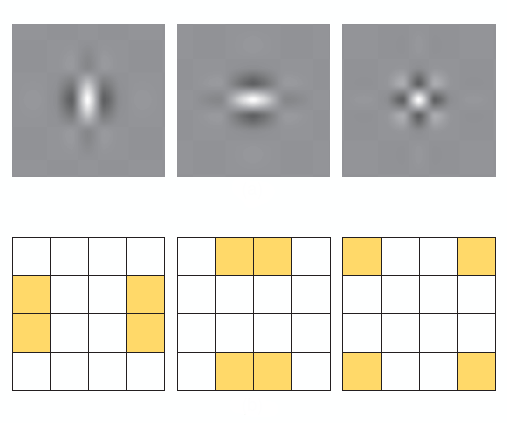
\includegraphics[width=0.5\textwidth]{litreview/images/dwt_wavelets.png}
    \mycaption{Typical wavelets from the 2D separable DWT\@}{Top: Wavelet point
      spread functions for $\psitd^v$ (low-high), $\psitd^h$ (high-low), and
      $\psitd^d$ (high-high) wavelets. High-high wavelets are in a checkerboard
      pattern, with no favoured orientation. Bottom: Idealized support of the
      spectra of each of the wavelets. Image taken from
      \cite{selesnick_dual-tree_2005}.}
      \label{fig:ch2:dwt_wavelets}
  \end{figure}
  % \begin{quote}
    % Always operate at the slowest possible sample rate.
  % \end{quote}

  \eqref{eq:ch2:2d_shifts} gave the equation for the daughter wavelets in 2-D,
  in 1-D at scales $a=2^j, j \geq 0$, this is simply:
  \begin{equation}
    \psiod_{b, j}(u) = 2^{-j/2} \psiod\left(\frac{u-b}{2^j} \right)
  \end{equation}
  The 2-D DWT has one scaling function and three wavelet functions, composed of
  the product of 1-D wavelets in the horizontal and vertical directions:
  \begin{align}
    \phitd(\xy) &= \phiod(u_1)\phiod(u_2) \label{eq:ch2:dwt1}\\
    \psitd^h(\xy) &= \phiod(u_1) \psiod(u_2) \\
    \psitd^v(\xy) & = \psiod(u_1) \phiod(u_2) \\
    \psitd^d(\xy) & = \psiod(u_1) \psiod(u_2) \label{eq:ch2:dwt4}
  \end{align}
  with $h, v, d$ indicating the sensitivity to horizontal, vertical and diagonal
  edges. The point spread functions for the wavelet functions are shown in
  \autoref{fig:ch2:dwt_wavelets}.
  
  For the four equations above \eqref{eq:ch2:dwt1} -- \eqref{eq:ch2:dwt4},
  define the daughter wavelets as:
  \begin{align}
    \phitd^j_{kl}(\xy) &= \phiod_{j,k}(u_1)\phiod_{j,l}(u_2) \\
    \psitd^{h,j}_{kl}(\xy) &= \phiod_{j,k}(u_1) \psiod_{j,l}(u_2) \\
    \psitd^{v,j}_{kl}(\xy) & = \psiod_{j,k}(u_1) \phiod_{j,l}(u_2) \\
    \psitd^{d,j}_{kl}(\xy) & = \psiod_{j,k}(u_1) \psiod_{j,l}(u_2) 
  \end{align}
  for $\alpha = \{h, v, d\},\ k,l \in \integers$ where $k,l$ define horizontal
  and vertical translation. We can then get an orthonormal
  basis with the set $\{ \phitd^j_{kl}, \psitd^{\alpha,j}_{kl} \}$.
  The wavelet coefficients at chosen scale and location can then be found by
  taking the inner product of the signal $x$ with the daughter wavelets.

  % A signal $x \in L_2(\reals[2])$ is represented at resolution $2^j$ by the
  % function $x_j = a_j + \sum_\alpha d^\alpha_j$, where:
  % \begin{align}
    % a_j &= \sum_
  % \end{align}

  \subsubsection{Shortcomings}
  The Discrete Wavelet Transform (DWT) is an orthogonal basis. It is a natural
  first signal expansion to consider when frustrated with the limitations of the
  Fourier Transform. It is also a good example of the limitations of
  non-redundant transforms, as it suffers from several drawbacks:
  \begin{itemize}
    \item The DWT is sensitive to the zero crossings of its wavelets. 
      We would like singularities in the input to yield large wavelet
      coefficients, but this may not always be the case.
      % if they fall at a zero crossing of a wavelet, the output can be small. 
      See
      \autoref{fig:ch2:dwt_zero_crossing}.
    \item They have poor directional selectivity. As the wavelets are purely
      real, they have passbands in all four quadrants of the frequency plane.
      While they can pick out edges aligned with the frequency axis, they are
      not specific to other orientations. See \autoref{fig:ch2:dwt_wavelets}.
    \item They are not shift invariant. In particular, small shifts greatly
      perturb the wavelet coefficients. \autoref{fig:ch2:dwt_zero_crossing} shows
      this for the centre-left and centre-right images.
      % \autoref{fig:ch2:dtcwt_shift_invariance} (right) also shows this.
  \end{itemize}

  The lack of shift invariance and the possibility of low outputs at
  singularities is a price to pay for the critically sampled property of the
  transform. This shortcoming can be overcome with the undecimated DWT
  \cite{mallat_wavelet_1998,coifman_translation-invariant_1995}, 
  but it comes with a heavy computational and memory cost. 

  \begin{figure}
    \centering
      \makebox[\textwidth][c]{%
        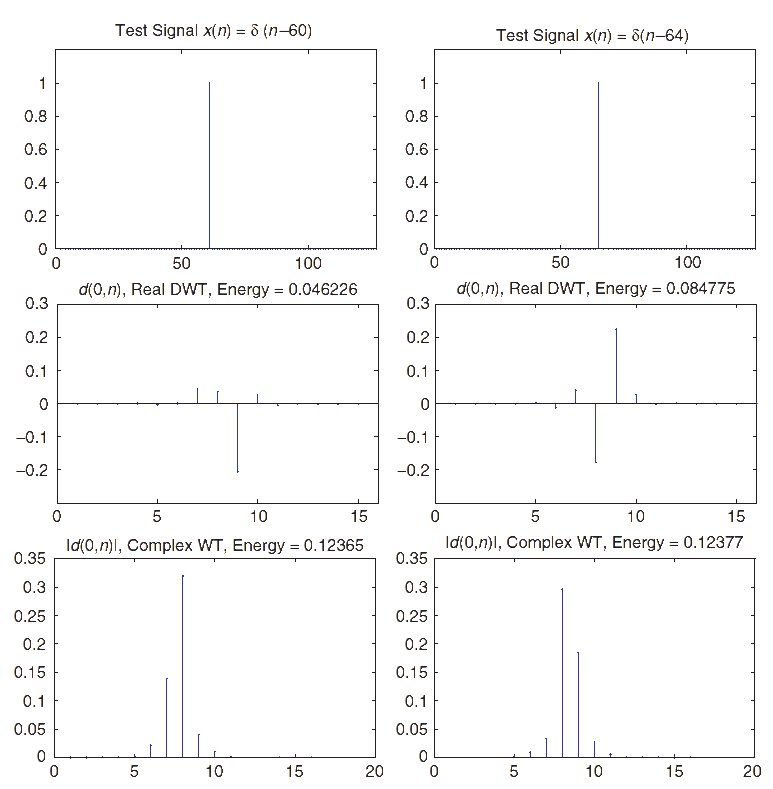
\includegraphics[width=1.1\textwidth]{litreview/images/dwt_zero_crossing.png}
      }
      \mycaption{Sensitivity of DWT coefficients to zero crossings and small
        shifts}{Two impulse signals $\delta(n-60)$ and $\delta(n-64)$ are
        shown (top), as well as the wavelet coefficients for scale $j=1$ for the DWT (middle) and
        for the $\DTCWT$ (bottom). In the middle row, not only are the coefficients very different
        from a shifted input, but the energy has almost doubled. As the DWT is an orthonormal
        transform, this means that this extra energy has come from other scales. In comparison, the
      energy of the magnitude of the $\DTCWT$ coefficients has remained far more constant, as has the
    shape of the envelope of the output.  Image taken from \cite{selesnick_dual-tree_2005}.}
      \label{fig:ch2:dwt_zero_crossing}
  \end{figure}

\subsection{Complex Wavelets}\label{sec:ch2:complex_wavelets}
  Fortunately, we can improve on the DWT with complex wavelets, as they can
  solve these new shortcomings while maintaining the desired localization
  properties. 
  
  The Fourier transform does not suffer from a lack of directional selectivity
  and shift variance, because its basis functions are based on the complex
  sinusoid: 
  \begin{equation} 
    e^{j\omega t} = \cos(\omega t) + j\sin(\omega t)
  \end{equation} 
  whereas the DWT's basis functions are based on only the real
  sinusoid $\cos(\omega t).$\footnote{we have temporarily switched to 1D
  notation here as it is clearer and easier to use, but the results still hold
  for 2D} As $t$ moves along the real line, the phase of the
  Fourier coefficients change linearly, while their magnitude remains constant. In
  contrast, as $t$ moves along the real line, the sign of the real coefficient
  flips between -1 and 1, and its magnitude is a rectified sinusoid.

  The nice properties of the complex sinusoids come from the fact that the
  cosine and sine functions of the Fourier transform form a Hilbert Pair and
  together constitute an analytic signal.

  We can achieve these nice properties if the mother wavelet for our wavelet
  transform is analytic:
  \begin{equation}
    \psiod_{c}(t) = \psiod_{r}(t) + j\psiod_{i}(t) \label{eq:ch2:complex_wavelet}
  \end{equation}
  where $\psiod_{r}(t)$ and $\psiod_{i}(t)$ form a Hilbert Pair (i.e.,\ they are
  $90\degs$ out of phase with each other).

  There are a number of possible ways to do a wavelet transform with complex
  wavelets. We examine two in particular, a Fourier-based, sampled CWT using
  Morlet wavelets, and the Dual-Tree Complex Wavelet Transform ($\DTCWT$)
  developed by Kingsbury \cite{kingsbury_wavelet_1997, kingsbury_dual-tree_1998,
  kingsbury_dual-tree_1998-1,  kingsbury_image_1999, kingsbury_shift_1999,
  kingsbury_dual-tree_2000, kingsbury_complex_2001, selesnick_dual-tree_2005}.

  We look at the Morlet wavelet transform because it is used by
  Mallat et.\ al.\ in their scattering transform
  \cite{bruna_classification_2011, bruna_invariant_2013, bruna_scattering_2013,
  oyallon_generic_2013, oyallon_deep_2015, sifre_rotation_2013,
  sifre_rigid-motion_2014, sifre_rigid-motion_2014-1, sifre_scatnet_2013}. 
  We believe the $\DTCWT$ 
  several advantages over the Morlet based implementation, and has been the
  basis for most of our work.

Let us write the wavelet transform of an input $x$ as 
\begin{equation}
  \mathcal{W}x = \left\{x \ast \phitd_J, x \ast \psitd_{\lambda}
  \right\}_{\lambda} \label{eq:ch2:wave2}
\end{equation}
where $\lambda = (j, k)$ indexes the $J$ scales and $K$ orientations of the
chosen wavelet transform, whether it be the $\DTCWT$ or Morlet transform.

\subsection{Sampled Morlet Wavelets}\label{sec:ch2:morlet_fourier}
  % Just need to review in Vetterli, how to do FFT based sampling of the CWT.
  The wavelet transform used by Mallat et.\ al.\ in their scattering transform is an efficient
  implementation of the Gabor Transform.  While the Gabor wavelets have the best
  theoretical trade-off between spatial and frequency localization, they have a
  (usually small) non-zero mean.  This violates \eqref{eq:ch2:admissibility} making them
  inadmissible as wavelets. Instead, the Morlet wavelet has the same shape, but
  with an extra degree of freedom chosen to set $\int \psitd (\bmu{u}) d\bmu{u}
  =0$. This wavelet has equation (in 2D):
  \begin{equation}
    \psitd(\bmu{u}) = \frac{1}{2\pi\sigma^2} {(e^{i\bmu{u}\xi} - \beta)}
                     e^{-\frac{|\bmu{u}|^2}{2\sigma^2}} 
    \label{eq:ch2:morlet}
  \end{equation}
  where $\beta$ is usually $<<1$ and is this extra degree of freedom, 
  $\sigma$ is the size of the gaussian window, and $\xi$ is the
  approximate location of the peak frequency response --- i.e.,\ for an octave based
  transform, $\xi = 3\pi/4$.

  \citeauthor{bruna_invariant_2013} add a further additional degree of freedom in their 
  original design \cite{bruna_invariant_2013} by allowing for a non-circular
  Gaussian window over the complex sinusoid, which gives control over the angular
  resolution of the final wavelet. \eqref{eq:ch2:morlet} now becomes:
  \begin{equation}
    \psitd(\bmu{u}) = \frac{\gamma}{2\pi\sigma^2}{(e^{i\bmu{u}\xi} - \beta)}
                  e^{-\bmu{u^t}\Sigma^{-1}  \bmu{u}} 
    \label{eq:ch2:morlet_slant}
  \end{equation}
  Where
  $$\Sigma^{-1} = \left[ \begin{smallmatrix} 
      \frac{1}{2\sigma^2} & 0 \\ 
      0 & \frac{\gamma^2}{2\sigma^2} 
      \end{smallmatrix} \right] $$
  The effects of modifying the eccentricity parameter $\gamma$ and the window size
  $\sigma$ are shown in \autoref{fig:ch2:morlet_filters}. A full family of
  Morlet wavelets at varying scales and orientations is shown in 
  \autoref{fig:ch2:morlet_littlewood_paley}.
  % To have a full two
  % dimensional wavelet transform, we need to rotate this mother wavelet by angle
  % $\theta$ and scale it by $j/Q$, where $Q$ is the number of scales per octave
  % (usually 1 in image processing). 

  % This can be done by doing the following
  % substitutions in \eqref{eq:ch2:morlet_slant}:
  % \begin{align*}
    % R_{\theta}& = \left[ \begin{smallmatrix}
                    % \cos(\theta) & -\sin(\theta) \\
                    % \sin(\theta) & \cos(\theta)
                  % \end{smallmatrix} \right] \\
    % \bmu{u}_{\theta} & =  R_{-\theta} \bmu{u} \\
    % \sigma_j & =  2^{\frac{j-1}{Q}} \sigma \\
    % \xi_j & =  \frac{\xi}{2^{\frac{j-1}{Q}}}
  % \end{align*}
  % We can combine these two variables into a single coordinate
  % \begin{equation}
    % \lambda = (\theta, j/Q)
  % \end{equation}
  % We can now scale and rotate this mother wavelet:
  % \begin{equation}
    % \psi_{\lambda}(\bmu{u}) = 2^{-j/Q}\psi(2^{-j/Q}R_{\theta}^{-1} \bmu{u})
  % \end{equation}
  \begin{figure}
    \begin{center}
      
\includegraphics[height=6cm]{\imgpath/morlet_filters.png}
      \mycaption{Single Morlet filter with varying slants and window sizes}
              {Top left --- $45\degs$ plane wave (real part only). Top right --- plane wave with
              $\sigma=3,\gamma=1$. Bottom left --- plane wave with $\sigma=3,\gamma=0.5$. Bottom
            right --- plane wave with $\sigma=2,\gamma=0.5$.}
      \label{fig:ch2:morlet_filters}
    \end{center}
  \end{figure}
  % \begin{figure}
    % \begin{center}
      % \makebox[\textwidth][c]{%
        % 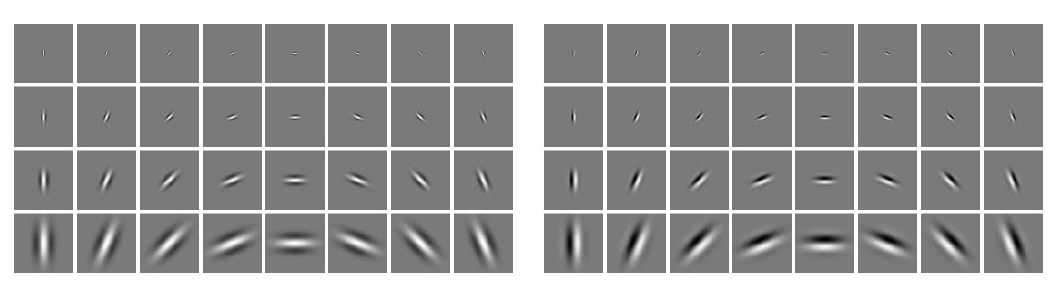
\includegraphics[width=1.1\textwidth]{\imgpath/morlet_wavelets_full.png}
      % }
      % \mycaption{The full dictionary of Morlet wavelets used by Mallat}
              % {The real filters are on the left and the imaginary on the right. The first row
              % correspond to scale $j=1$, increasing up to $j=4$. The first column corresponding to
            % $\theta = 0$, rotating through $\pi/8$ up to the eighth column of $7\pi/8$,
          % $\gamma=1/2$.} 
      % \label{fig:ch2:morlet_wavelets_full}
    % \end{center}
  % \end{figure}

\subsubsection{Tightness and Invertibility}
Recall our definition of the wavelet transform $\mathcal{W}$ from \eqref{eq:ch2:wave2}.

Assuming the transform is bounded, we can always scale it so that it satisfies
Plancherel's equality
\begin{equation}
  \norm{\mathcal{W}x} = \norm{x}
\end{equation}
which is a nice property to have for invertibility, as well as for analysing
how different signals get transformed (e.g.\ white noise versus standard
images). Scaling the transform changes the upper bound $B$ in \eqref{eq:ch2:frame_bounds} 
to 1 and makes the lower bound $A = 1-\alpha$, where $\alpha$ is a measure of how
non-tight a frame is.
  
Let us look at the tightness of a Morlet wavelet frame for a few manually selected parameters. 
\begin{itemize}
  \item For dilations, we choose $a = 2^{-j/Q}$ for $j\in \mathbb{Z}$
    controlling the scale and $Q$ the number of octaves per scale.
  \item For rotations, we subdivide the interval $[0, \pi)$ into $K$ sections,
    and choose $\theta_k = \frac{k\pi}{K},\ k = \{0, 1, \ldots K-1\}$.
  \item For the translations, we set the sample spacing $\Delta \bmu{b} =
    2^{-j/Q}$. \textbf{Need to check this} 
\end{itemize}
  
Using the capital notation to denote the Fourier transform, define the function
$A(\ww)$ to be the coverage each wavelet family has over the frequency plane: 
\begin{equation}
  A(\ww) = {|\Phi_J(\ww)|}^2 + \sum_{\lambda} {|\Psi_{\lambda}(\ww)|}^2
  \label{eq:ch2:lwood_paley}
\end{equation}
For a unit norm input $||x||^2 = 1$ and scaled wavelets, we can now change
\eqref{eq:ch2:frame_bounds} to be:
\begin{equation}
  1-\alpha \leq A(\ww) \leq 1
\end{equation}
  If $A(\ww)$ is ever close to 0, then there is not a good coverage of the frequency plane
  at that location. 
  % If it ever exceeds 1, then there is overlap between bases.
  % Both of these conditions make invertibility difficult\footnote{In practise,
  % if $A(\ww)$ is only slightly greater 1 for only a few small areas of
  % $\ww$, approximate inversion can be achieved}.
  \autoref{fig:ch2:morlet_littlewood_paley} show the frequency coverage of a few
  sample grids over the CWT parameters used by \Mallat. Invertibility is possible, but not
  guaranteed for all configurations. 
  
  % The Fourier transform of the inverse
  % filters are defined by:
  % \begin{align}
    % \mathcal{F}\phiod_J^{-1}(\omega) &= A(\omega)^{-1} \mathcal{F}\phiod_J(\omega) \\
    % \mathcal{F}\psi_{\lambda}^{-1}(\omega) &= A(\omega)^{-1}
      % \mathcal{F}\psi_{\lambda}(\omega) 
  % \end{align}

  \begin{figure}
    \centering
      \makebox[\textwidth][c]{%
        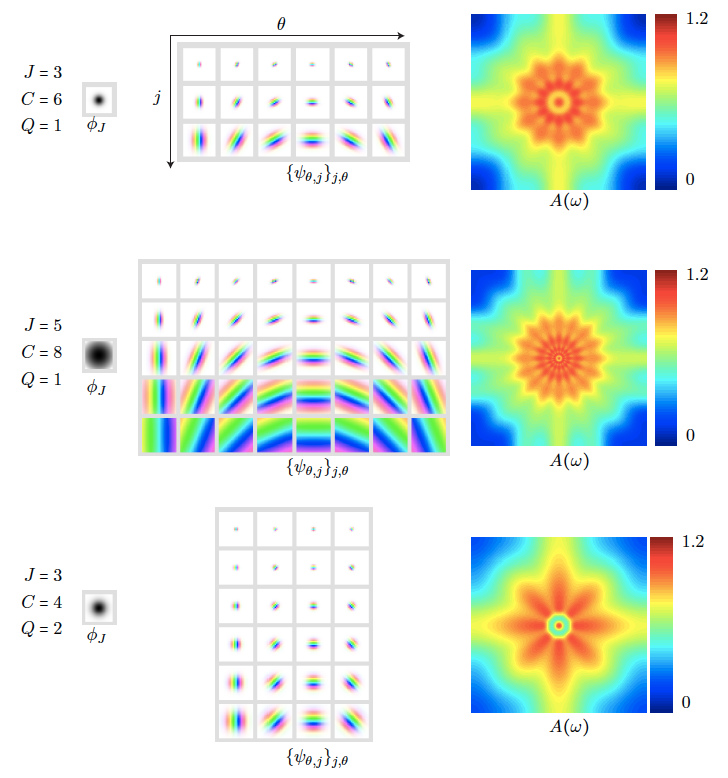
\includegraphics[width=1.1\textwidth]{\imgpath/morlet_littlewood_paley.png}
      }
      \mycaption{Three Morlet Wavelet families and their tiling of the frequency
              plane}{For each set of parameters, the point spread functions of
              the wavelet bases are shown, next to their covering of the
              frequency plane $A(\ww)$. None of the configurations cover the corners of the
              frequency plane, but this is often mostly noise. 
              Increasing $J$, $K$ (Sifre uses $C$ in these
              diagrams) or $Q$ gives better frequency localization but at the
              cost of spatial localization and added complexity. Image taken
              from \cite{sifre_rigid-motion_2014-1}. \textbf{TODO: update figure
              to show only the real wavelets in black and white and the correct
              variable names}.}
      \label{fig:ch2:morlet_littlewood_paley}
  \end{figure}

% The discrete wavelet transform (DWT) provides a non-redundant representation
  % of

% signals, hence overcomes the problem of redundancy. The DWT samples the
% timefrequency
% plane and only preserves the least number of the discrete coefficients
% that are required for perfect synthesis. The scale parameter a is sampled first
% on a logarithmic grid, and then the time parameter b is sampled with respect to
% the scale parameter. Though any sampling rate is possible, the DWT is mostly
% computed on the dyadic grid such that the DWT can be efficiently implemented
% by filter bank trees. This is of real value for practical applications.
% Figure 3.1 shows the diagram for a 4-level forward and inverse DWT, which
% explains how the DWT can be efficiently implemented by octave-band,
% discretetime
% filter bank trees. The notations in the diagram have the following meanings:
% 1. x is the original signal
% 2. ˆx is the reconstructed signal
% 3. H0 is the low-pass decomposition filter
% 4. H1 is the high-pass decomposition filter
% 5. °#2 is the operation that downsamples the signal by 2
% 6. G0 is the low-pass reconstruction filter
% 7. G1 is the high-pass reconstruction filter
% 8. °"2 is the operation that upsamples the signal by 2 by inserting zeros
% 9. w(j) are the wavelet coefficients in the j-th subband.
% The decomposition filter (H0, H1) and reconstruction filters (G0, G1) are
% carefully
% chosen in order that the wavelet transform can be inverted, i.e. x = ˆx. The
% above procedure can be represented by matrix-vector notations, which will later
% be introduced in 3.2.3.
% 
\subsection{The $\DTCWT$}
  The $\DTCWT$ was first proposed by \citeauthor{kingsbury_dual-tree_1998} in
  \cite{kingsbury_dual-tree_1998, kingsbury_dual-tree_1998-1} as a way to combat
  many of the shortcomings of the DWT, in particular, its poor directional
  selectivity, and its poor shift invariance. A thorough analysis of the
  properties and benefits of the $\DTCWT$ is done in
  \cite{kingsbury_image_1999,selesnick_dual-tree_2005}. Building on these
  properties, it been used
  successfully for denoising and inverse problems \cite{rivaz_bayesian_2001,
  zhang_bayesian_2008, zhang_variational_2015, miller_image_2008}, texture
  classification \cite{hatipoglu_texture_1999, rivaz_complex_1999}, image
  registration \cite{loo_motion-estimation-based_2001, chen_efficient_2012}
  and SIFT-style keypoint generation matching \cite{fauqueur_multiscale_2006,
  anderson_determining_2005, anderson_rotation-invariant_2006,
  bendale_multiscale_2010, ng_robust_2012} amongst many other applications. 
  Compared to Gabor (or Morlet) image analysis, the authors of
  \cite{selesnick_dual-tree_2005} sum up the dangers as:
  \begin{quote}
    A typical Gabor image analysis is either expensive to compute, is
    noninvertible, or both.
  \end{quote}
  This nicely summarises the difference between this method and the Fourier
  based method outlined in \autoref{sec:ch2:morlet_fourier}. The $\DTCWT$ is
  a filter bank (FB) based wavelet transform. It is faster
  to implement than the Morlet analysis, as well as being more readily invertible.

\subsubsection{Deisgn Criteria for the $\DTCWT$}
  As in \autoref{sec:ch2:complex_wavelets}, we want to have a complex mother
  wavelet $\psiod_c = \psiod_r + j\psiod_i$ and complex scaling function $\phiod_c =
  \phiod_r + j\phiod_i$, but now achieved with filter banks. The complex componenet
  allows for support of both the wavelet and scaling functions on only one half of
  the frequency plane. 
  
  The dual tree framework shown in \autoref{fig:ch2:dtcwt_1d_fb} can achieve this 
  by making the real and imaginary components with their own DWT. In particular, if
  we define:
  \begin{itemize}
    \item $h_0, h_1$ the low and high-pass analysis filters for $\phiod_r, \psiod_r$  
    \item $g_0, g_1$ the low and high-pass analysis filters for $\phiod_i, \psiod_i$
    \item $\tilde{h}_0, \tilde{h}_1$ the low and high pass synthesis filters
      for $\tilde{\phiod}_r, \tilde{\psiod}_r$.
    \item $\tilde{g}_0, \tilde{g}_1$ the low and high pass synthesis filters for
      $\tilde{\phiod}_i, \tilde{\psiod}_i$.
  \end{itemize}

  The dilation and wavelet equations for a 1D filter bank implementation are:
  \begin{align}
    \phiod_r(t) & =  \sqrt{2} \sum_n h_0(n) \phiod_r(2t-n) \\
    \psiod_r(t) & =  \sqrt{2} \sum_n h_1(n) \phiod_r(2t-n) \\
    \phiod_i(t) & =  \sqrt{2} \sum_n g_0(n) \phiod_i(2t-n) \\
    \psiod_i(t) & =  \sqrt{2} \sum_n g_1(n) \phiod_i(2t-n) 
  \end{align}

  \begin{figure}
    \centering
      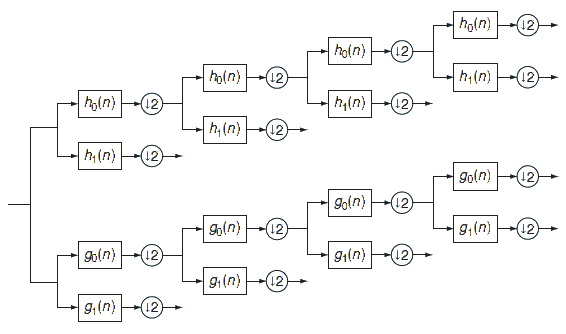
\includegraphics[width=\textwidth]{\imgpath/dtcwt_1d_fb.png}
      \mycaption
      {Analysis FB for the $\DTCWT$}{Top `tree' forms the real component of the
      complex wavelet $\psiod_r$, and the bottom tree forms the imaginary (Hilbert
      pair) component $\psiod_i$. Image taken from
      \cite{selesnick_dual-tree_2005}.}
      \label{fig:ch2:dtcwt_1d_fb}
  \end{figure}

  Designing a filter bank implementation that results in Hilbert symmetric
  wavelets does not appear to be an easy task. However, it was shown
  by \citeauthor{kingsbury_image_1999} in \cite{kingsbury_image_1999} (and later proved by
  \citeauthor{selesnick_hilbert_2001} in \cite{selesnick_hilbert_2001}) that the
  necessary conditions are conceptually very simple. One low-pass filter must be
  a \emph{half-sample shift} of the other. I.e., if $g_0(n) = h_0(n-1/2)$ then
  the corresponding wavelets are a Hilbert transform pair
  \begin{equation}
    \psiod_g(t) \approx \mathcal{H}\{\psiod_h(t)\}
  \end{equation}
  As the $\DTCWT$ is designed as an invertible filter bank implementation, this
  is only one of the constraints. As with convential (real) discrete wavelets,
  there are also perfect reconstruction, finite support, linear phase and
  vanishing moment constraints to consider in the filter bank design.

  The derivation of the filters that meet these conditions is covered in
  detail in \cite{kingsbury_complex_2001, kingsbury_design_2003}, and in
  general in \cite{selesnick_dual-tree_2005}. The result is the
  option of three main families of filters: biorthogonal filters ($h_0[n] =
  h_0[N-1-n]$ and $g_0[n] = g_0[N-n]$), q-shift filters ($g_0[n]
  = h_0[N-1-n]$), and common-factor filters. 
  
\subsubsection{2-D $\DTCWT$ and its Properties}
  While analytic wavelets in 1D are useful for their shift invariance, the real
  beauty of the $\DTCWT$ lies in its ability to make a separable 2D wavelet
  transform with oriented wavelets. 
  
  Figure~\autoref{fig:ch2:dwt_hh} shows the spectrum of
  the wavelet when the separable product uses purely real wavelets, as is the
  case with the DWT\@. Figure~\autoref{fig:ch2:dtcwt_hh} however, shows the separable
  product of two complex, analytic wavelets resulting in a localized and
  oriented 2D wavelet. 

  Note that in this thesis, we name the wavelets by the direction of the edge
  that they are most sensitive to. 
  
  For example, the $135\degs$ wavelet can be obtained by the separable product:
  \begin{align}
    \psitd(\xy) &= \psiod_c(u_1) \psiod_c^*(u_2) \label{eq:ch2:wavelet_separable_product}\\
              &= \left(\psiod_r(u_1) + j\psiod_i(u_1)\right) 
                 \left(\psiod_r(u_2) - j\psiod_i(u_2)\right) \\
              &= \left(\psiod_r(u_1)\psiod_r(u_2) + \psiod_i(u_1)\psiod_i(u_2)\right) 
                +j \left(\psiod_r(u_1)\psiod_i(u_2) - \psiod_i(u_1)\psiod_r(u_2)\right) 
                \label{eq:ch2:dtcwt_2d_product}
  \end{align}
  Similar equations can be obtained for the other five wavelets and the scaling
  function, by replacing $\psiod$ with $\phiod$ for each direction in turn (but not both
  together), and not taking the complex conjugate
  in \eqref{eq:ch2:wavelet_separable_product} to get the filters in the
  right-hand half of the frequency plane. The 2-D $\DTCWT$ requires four 2-D
  DWTs to calculate the four possible combinations of real and imaginary
  components. The high and lowpass outputs from these DWTs can then be summed in
  different ways as in \eqref{eq:ch2:dtcwt_2d_product} to get the complex
  bandpass wavelets.  \autoref{fig:ch2:dtcwt_wavelets} shows the resulting
  wavelets both in the spatial domain and their idealized support in the
  frequency domain.

  \begin{figure}
%      \centering
      \subfloat[]{\makebox[\textwidth][c]{%
        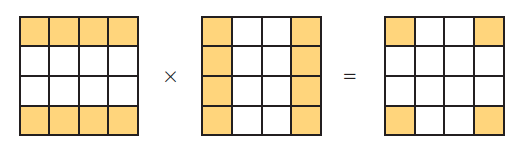
\includegraphics[width=0.6\textwidth]{\imgpath/dwt_hh.png}
        \label{fig:ch2:dwt_hh}}}
      \newline
      \subfloat[]{\makebox[\textwidth][c]{%
        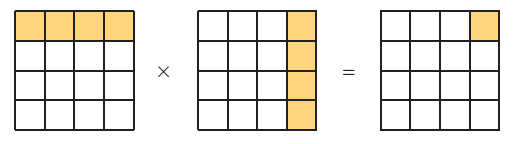
\includegraphics[width=0.6\textwidth]{\imgpath/dtcwt_hh.png}
        \label{fig:ch2:dtcwt_hh}}}
      \mycaption{The DWT high-high vs the $\DTCWT$ high-high frequency support}
              {\subref{fig:ch2:dwt_hh} The high-high DWT wavelet having a passband in
              all 4 corners of the frequency plane vs \subref{fig:ch2:dtcwt_hh} the
              high-high $\DTCWT$ wavelet frequency support only existing in one
              quadrant. Taken from \cite{selesnick_dual-tree_2005}}
      \label{fig:ch2:dwt_dtcwt_hh}
  \end{figure}
  \begin{figure}
    \centering
      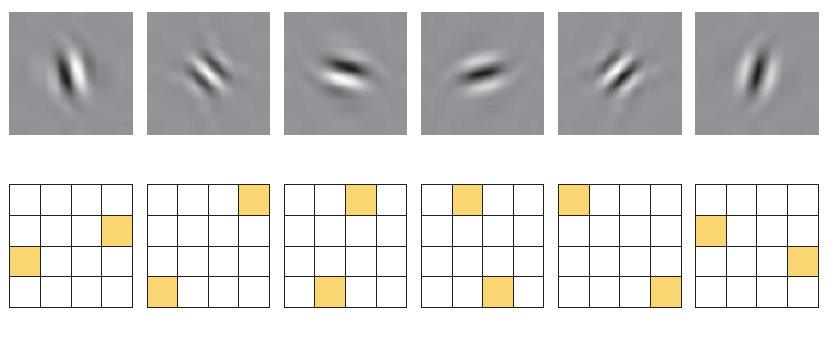
\includegraphics[width=\textwidth]{\imgpath/dtcwt_wavelets.png}
    \mycaption{Wavelets from the 2d $\DTCWT$}{\textbf{Top:} The six  oriented filters
      in the space domain (only the real wavelets are shown). From left to right
      these are the $105\degs, 135\degs, 165\degs, 15\degs, 45\degs, 75\degs$
      wavelets. \textbf{Bottom:}
      Idealized support of the Fourier spectrum of each wavelet in the 2D
      frequency plane. Spectra of the the real wavelets are shown --- the
      spectra of the complex wavelets ($\psiod_r + j\psiod_i$) only has support in the top
      half of the plane. Image taken from \cite{selesnick_dual-tree_2005}.}
      \label{fig:ch2:dtcwt_wavelets}
  \end{figure}

\subsubsection{Tightness and Invertibility}
  We analysed the coverage of the frequency plane for the Morlet wavelet family
  and saw what areas of the spectrum were better covered than others. How about
  for the $\DTCWT$?

  It is important to note that in the case of the q-shift $\DTCWT$, the wavelet
  transform is also approximately unitary, i.e.,\
  \begin{equation}
    \norm{x}^2 \approx \norm{\mathcal{W}x}^2
  \end{equation}
  and the implementation is perfectly invertible as $A(\ww)$ from
  \eqref{eq:ch2:lwood_paley}
  function is unity (or very near unity) $\forall \ww \in [-\pi, \pi]\x [-\pi,
  pi]$. See
  \autoref{fig:ch2:dtcwt_lwoodpaley}. This is not a surprise, as it is a design
  constraint in choosing the filters, but nonetheless is important to note. 

  % A beneficial property of energy conservation is that the noise in the input
  % will equal the noise in the wavelet coefficients. When we introduce
  % Scatternets, we can show that we can keep the unitary property in the
  % scattering coefficients. 
  % This is an important property, particularly in light
  % of the recent investigations in \cite{szegedy_intriguing_2013}. This paper
  % saw that it is easy to find cases in CNNs where a small amount of input
  % perturbation results in a completely different class label (see
  % \autoref{fig:ch2:difference}). Having a unitary transform limits the
  % amount the features can change, which will make the entire network more
  % stable to distortion and noise.

  \begin{figure}
    \subfloat{\makebox[0.6\textwidth][c]{%
      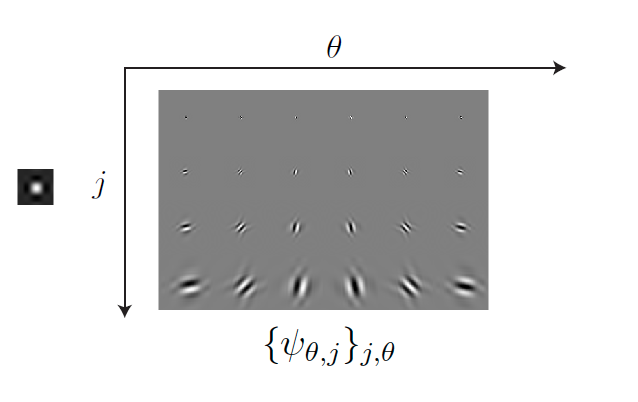
\includegraphics[width=0.7\textwidth,valign=c]{\imgpath/dtcwt_real_4scales.png}
    }}
    \subfloat{\makebox[0.4\textwidth][c]{%
      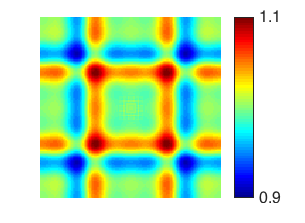
\includegraphics[width=0.5\textwidth,valign=c]{\imgpath/dtcwt_lwoodpaley_2.png}
    }}
    \mycaption{$\DTCWT$ family for $J=4$ and their frequency coverage}{
    Note the reduced scale compared to \autoref{fig:ch2:morlet_littlewood_paley}.}
    \label{fig:ch2:dtcwt_lwoodpaley}
  \end{figure}

\subsection{Summary of Methods}
  One final comparison to make between the $\DTCWT$ and the Morlet wavelets is
  their frequency coverage. The Morlet wavelets have flexibility at the cost of 
  computational expense, and can be made to have tighter angular resolution than
  the $\DTCWT$. However it is not always
  better to keep using finer and finer resolutions, indeed the Fourier
  transform gives the ultimate in angular resolution, but as mentioned, this
  makes it less stable to shifts and deformations. We will explore this in more
  depth in Chapter 3.

  % \autoref{tab:dtcwt_vs_dwt_vs_mallat} compares the advantages and
  % disadvantages of the wavelet methods discussed in this chapter.
  % \begin{figure}
    % \subfloat[$\DTCWT$ wavelets (left to right) --- $15\degs$, $45\degs$ and $75\degs$]{%
      % \makebox[\textwidth][c]{%
      % 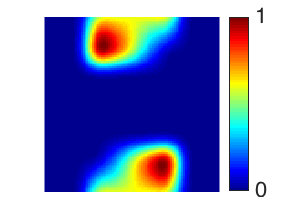
\includegraphics[width=0.4\textwidth]{\imgpath/dtcwt_15deg_energy.png}
      % 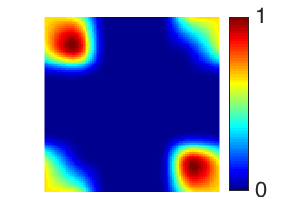
\includegraphics[width=0.4\textwidth]{\imgpath/dtcwt_45deg_energy.png}
      % 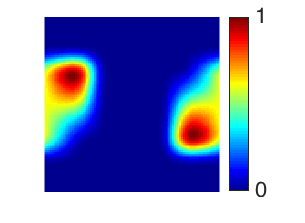
\includegraphics[width=0.4\textwidth]{\imgpath/dtcwt_75deg_energy.png}
    % }}
    % \newline
    % \subfloat[Morlet wavelets (left to right) --- $0\degs$, $45\degs$, $90\degs$] 
      % $67.5\degs$,  and $90\degs$]{%
      % \makebox[\textwidth][c]{%
      % 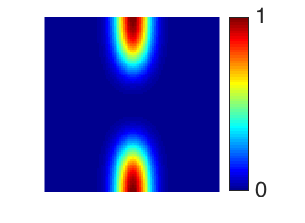
\includegraphics[width=0.4\textwidth]{\imgpath/mallat_0deg_energy.png}
      % 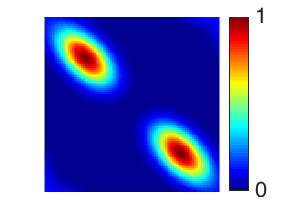
\includegraphics[width=0.4\textwidth]{\imgpath/mallat_45deg_energy.png}
      % 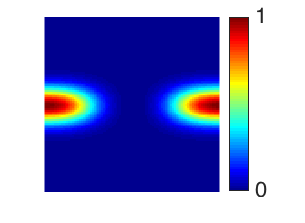
\includegraphics[width=0.4\textwidth]{\imgpath/mallat_90deg_energy.png}
    % }}
    % \newline
    % \subfloat[]{%
      % % Use two makebox commands to center the images
      % \makebox[0.5\textwidth][c]{%
        % \hspace{1cm}
        % 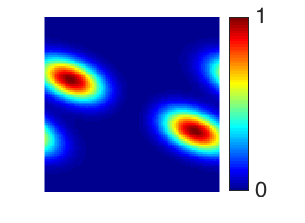
\includegraphics[width=0.4\textwidth,center]{\imgpath/mallat_675deg_energy.png}
      % }
      % \makebox[0.5\textwidth][c]{%
        % \hspace{-1cm}
        % 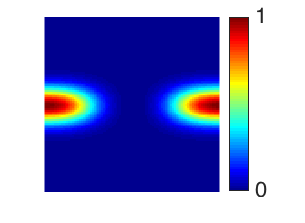
\includegraphics[width=0.4\textwidth,center]{\imgpath/mallat_90deg_energy.png}
      % }
    % }
    % \mycaption{Comparison of the energy spectra for $\DTCWT$ wavelets to Morlet
    % wavelets}{Normalized Energy spectra of the $\DTCWT$ wavelets versus the preferred
          % 8 orientation Morlet wavelets by Mallat for the second quadrant.
          % Orientations listed refer to the edge orientation in the spatial
          % domain that gives the highest response. All wavelets have been
          % normalized to be between zero and one.
          % The Morlet wavelets have finer angular
          % resolution, which can give better discrimination, at the cost of
          % decreasing stability to deformations, and requiring larger spatial
          % support.}
    % \label{fig:ch2:wavelet_freq_resp}
  % \end{figure}

\section{Scatternets}\label{ch:scatternets}
% Let us define the pairs of authors here
  Scatternets have been a very large influence on
  our work, as well as being quite distinct from the previous discussions on
  learned methods. They were first introduced by  
  \citeauthor{bruna_classification_2011} in their work 
  \cite{bruna_classification_2011}, and then were rigorously defined by Mallat
  in \cite{mallat_group_2012}.   

  While CNNs have the ability to learn invariances to nuiscance variabilities, 
  the properties and optimal configurations are not well understood. 
  It typically takes multiple trials
  by an expert to find the correct hyperparameters for these networks. A
  scattering transform instead builds well understood and well defined invariances. 
  
  We first review some of the desirable invariances before describing how a
  ScatterNet achieves them.

\subsection{Desirable Properties}
\subsubsection{Translation Invariance}
  Translation is often defined as being uninformative for classification --- an
  object appearing in the centre of the image should be treated the same way as
  an the same object appearing in the corner of an image, i.e.,\ a
  representation $\Phi x$ is invariant to global translations $x_c(\bmu{u}) =
  x(\bmu{u}-\bmu{c})$ by 
  $\bmu{c}=(c_1,c_2) \in \mathbb{R}^2$ if
  % The first requirement for Scatternets - translation invariance
  \begin{equation}\label{eq:scat_trans_invariance}
    \norm{\Phi x_c - \Phi x} \leq C
  \end{equation}
  for some small constant $C>0$.
  Note that we may instead want only local translation invariance and
  restrict the distance $|\bmu{c}|$ for which \eqref{eq:scat_trans_invariance}
  is true. 
  
  Note that CNNs are naturally covariant to translations in the pixel space, 
  so $\Phi x_c = (\Phi x)_c,\ \bmu{c} \in \mathbb{Z}^2$. Of course, natural objects
  exist in continuous space and are sampled, and any two images of the same
  scene taking with small camera disturbances are unlikely to be at integer pixel 
  shifts of each other.

\subsubsection{Stability to Noise}
  Stability to additive noise is another useful invariance to build,
  as it is a common feature in sampled signals. Stability is defined in terms of
  Lipschitz continuity, which is a strong form of uniform continuity for
  functions, which we briefly introduce here.

  Formally, a Lipschitz continuous function is limited in how fast it can change;
  there exists an upper bound on the gradient the function can take, although it
  doesn't necessarily need to be differentiable everywhere. The modulus operator
  $|x|$ is a good example of a function that has a bounded derivative and so is
  Lipschitz continuous, but isn't differentiable everywhere. Alternatively, the
  modulus squared has derivative everywhere but is not Lipshitz continuous as
  its gradient grows with $x$.

  \begin{figure}
    \begin{center}
      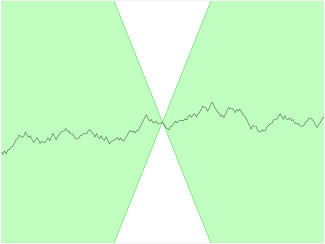
\includegraphics[scale=0.6]{\imgpath/Lipschitz_continuity.png}
      \mycaption{A Lipschitz continuous function}{There is a cone for this
              function (shown in white) such that the graph always remains entirely outside
              the cone as it is shifted across. The minimum gradient needed for this to hold
              is called the `best Lipschitz constant'.}
      \label{fig:lipschitz}
    \end{center}
  \end{figure}

  To be stable to additive noise, we require that for 
  a new signal $x'(\bmu{u}) = x(\bmu{u}) + \epsilon(\bmu{u})$, there must exist
  a bounded $C>0$ s.t.
  % The second requirement - noise stability
  \begin{equation}\label{eq:scat_noise_stability}
    \|\Phi x' - \Phi x\| \leq C \|x' - x\|
  \end{equation}

\subsubsection{Stability to Deformations}
  Small deformations are important to be invariant to. However, this must be
  limited. It is important to ignore intra-class variations 
  but not so invariant that an object can
  morph into another (in the case of MNIST for example, we do not want to be so
  stable to deformations that 7s can map to 1s). 
  
  Formally, for a new signal
  $x_{\tau}(\bmu{u}) = x(\bmu{u}-\tau(\bmu{u}))$, where $\tau(\bmu{u})$ is a non
  constant displacement field (i.e.,\ not just a translation) that deforms the
  image, we require a $C_\tau>0$ s.t.
  % The third requirement - deformation stability
  \protect\begin{equation}\label{eq:scat_deformation_stability}
    \|\Phi x_{\tau} - \Phi x \| \leq C_\tau \|x\| \sup_{\bmu{u}} |\nabla\tau(\bmu{u})|
  \protect\end{equation}
  The term on the right $|\nabla\tau(\bmu{u})|$ measures the deformation
  amplitude, so the supremum of it is a limit on the global defomation amplitude.

\subsection{Definition}
  A Fourier modulus satisfies the first two of these requirements, in that it is
  both translation invariant and stable to additive noise, but it is unstable to
  deformations due to the infinite support of the sinusoid basis functions it
  uses. It also loses too much information --- very different signals can all
  have the same Fourier modulus, e.g.\ a chirp, white noise and the Dirac delta
  function all have flat spectra.

  Another translation invariant and stable operator is the averaging kernel, and
  \Mallat\ use this to make the zeroth scattering coefficient:
  \begin{equation}
    S[\emptyset]x \definedas x \conv \phitd_J\left(2^J \bmu{u}\right)
  \end{equation}
  which is translation invariant to shifts less than $2^J$. It unfortunately
  results in a loss of information due to the removal of high frequency content.
  This is easy to see as the wavelet operator 
  $Wx = \{ x \conv \phitd_J, x \conv \psitd_\lambda \}_\lambda$
contains all the information of $x$, whereas the zeroth scattering coefficient
is simply the lowpass portion of $W$. 

This high frequency content can be `recovered' by keeping the wavelet
coefficients. The wavelet terms, like a convolutional layer in a CNN, is only
covariant to shifts rather than invariant. This covariance happens in the real 
and imaginary parts which both vary rapidly. Fortunately, its modulus is much
smoother and gives a good measure for the frequency-localized energy content at
a given spatial location\footnote{Interestingly, the modulus operator can often still be
inverted, and hence does not lose any information, due to the redundancies of
the complex wavelet transform \cite{waldspurger_phase_2012}}. Unlike
the Fourier modulus, the complex wavelet modulus is stable to deformations due
to the grouping together frequencies into dyadic packets
\cite{mallat_group_2012}. 

We combine the wavelet transform and modulus operators into one operator
$\tilde{W}$:
\begin{align}
  \tilde{W}x &= \{ x \conv \phitd_J,\ |x \conv \psitd_\lambda| \}_\lambda \label{eq:ch2:wave3}\\
             &= \{ x \conv \phitd_J,\ U[\lambda]x \}_\lambda 
\end{align}
where the $U$ terms are called the \emph{propagated} signals and $\lambda =
(j,k)$ indexes the scale and orientation of wavelet used.
These $U$ terms are invariant for shifts of up to $2^j$. \Mallat\ choose to
keep the same level of invariance as the zeroth order coefficients ($2^J$) 
by further averaging. This makes the first ordering scattering coefficients:
\begin{equation}
  S[\lambda_1]x \definedas U[\lambda_1]x \conv \phitd_J
  = |x \conv \psitd_{\lambda_1}| \conv \phitd_J
\end{equation}
Again this averaging comes at a cost of discarding high frequency information,
this time about the wavelet sparsity signal $U[\lambda] = |x \conv
\psi_\lambda|$ instead of the input signal $x$. We can recover this information
by repeating the above process. 
\begin{align}
  S[\lambda_1, \lambda_2]x &\definedas U[\lambda_2]U[\lambda_1]x \\
                           &=||x \conv \psitd_{\lambda_1}| \conv \psitd_{\lambda_2}| \conv \phitd_J
\end{align}
In general, let $p=(\lambda_1, \lambda_2, \ldots \lambda_m)$ be a path of length
$m$ describing the order of application of wavelets, and define:
\begin{align}
  U[p]x &= U[\lambda_m]U[\lambda_{m-1}]\cdots U[\lambda_1]x \\
        &= || \cdots |x \conv \psitd_{\lambda_1}| \conv \psitd_{\lambda_2} | \cdots
  \conv \psitd_{\lambda_m}|
\end{align}
and the $m$th order scattering coefficient along the path $p$ is $S[p]x = U[p]x
\conv \phitd_J$. Further, let $p+\lambda = (\lambda_1, \lambda_2, \ldots
\lambda_m, \lambda)$.  This allows us to recursively define the next set of
\emph{propagated} and \emph{scattering} coefficients by using $\tilde{W}$:
\begin{equation}
  \tilde{W}U[p]x = \{ S[p]x,\ U[p+\lambda]x \}_\lambda \label{eq:ch2:recursive}
\end{equation}
which is shown in \autoref{fig:ch2:scatternet_mallat}
  \begin{figure}
    \centering
      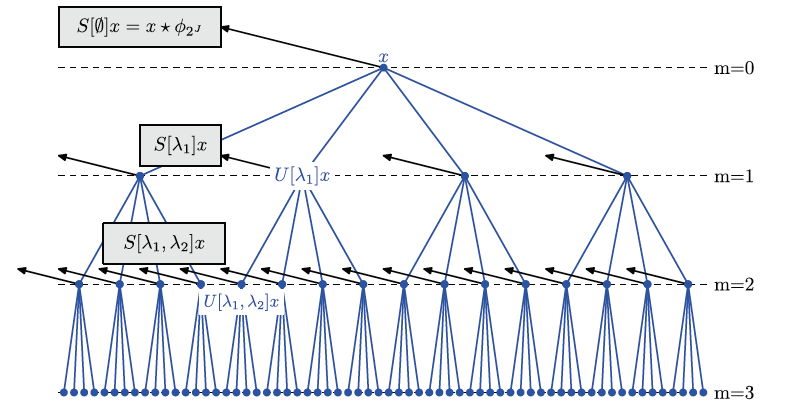
\includegraphics[width=\textwidth]{\imgpath/scatternet_diagram.png}
      \mycaption{The Scattering Transform}{Scattering outputs
               are the leftward pointing arrows $S[p]x$, and the intermediate 
               coefficients $U[p]x$ are the centre nodes of the tree. Taken
               from \cite{bruna_invariant_2013}.}
      \label{fig:ch2:scatternet_mallat}
  \end{figure}

\subsection{Resulting Properties}
For ease, let us define the `$m$th order scattering coefficients' as $S_m$ which
is the set of all coefficients with path length $m$. Further let $S$ be the set
of all scattering coefficients of any path length. The energy $\energy{Sx}$ we 
then define as
\begin{equation}
  \energy{Sx} = \sum_p \energy{S[p]x}
\end{equation}
We can make $W$ non-expansive with appropriate scaling. Further, define the energy $\energy{Wx}$ as
\begin{equation}
  \energy{Wx} = \energy{x\conv \phitd} + \sum_\lambda \energy{x \conv
  \psitd_\lambda} 
\end{equation}
then by Plancherel's formula
\begin{equation}
  (1-\epsilon)\energy{x} \leq \energy{Wx} \leq \energy{x}
\end{equation}
For the Morlet wavelets originally used in \cite{bruna_invariant_2013},
$\epsilon=0.25$, for the $\DTCWT$ $\epsilon = 0$.


\subsubsection{Translation Invariance}
\newcommand{\shift}{\mathcal{L}_c}

This is proven in section 2.4 of \cite{mallat_group_2012}. We
have so far described the Scattering representation as being `translation
invariant for shifts up to $2^J$'. We formalize this statement here.

For a 2-D averaging filter based on a father wavelet $\phitd$, 
$\phitd_J = 2^{-J}\phitd\left(2^{-J}\xy\right)$ it is proven in Appendix B of
\cite{mallat_group_2012} that shifting 
it by $\bmu{c}$, which we denote as $\mathcal{L}_c$, is Lipschitz continuous:
\begin{equation}
  \norm{\shift \phi_J - \phi_J} \leq 2^{-J+2}\lnorm{\nabla \phitd}{1}|\bmu{c}|
\end{equation}
where $\lnorm{\nabla \phitd}{1}$ is the $\ell_1$ norm of the grad of $\phitd$.

For simplicity, let us define $A_J x = \phitd_J \conv x$ and $Sx = A_J Ux$. Then we get:
\begin{align}
  \norm{S\shift x - Sx} & = \norm{\shift A_J Ux - A_J Ux} \\
                         &\leq \norm{\shift A_j - A_j}\norm{Ux} \\
                         & \leq 2^{-J+2}\lnorm{\nabla \phitd}{1}|\bmu{c}|\norm{x}
\end{align}
% as $\norm{Ux} \leq \norm{x}$. 

\subsubsection{Stability to Noise}
As $W$ is non-expansive and the complex modulus is also non-expansive
\begin{equation}
  \norm{\tilde{W}x - \tilde{W}y} \leq \norm{x-y}
\end{equation}
As we have already shown that $S$ is the repeated application of $\tilde{W}$ in
\eqref{eq:ch2:recursive}, we can then say
\begin{equation}
  \norm{Sx - Sy} \leq \norm{x-y}
\end{equation}
making scattering non-expansive and stable to noise.

\subsubsection{Stability to deformations}
From \cite{mallat_group_2012}, if $\mathcal{L}_\tau x = x(\xy -\tau(\xy))$ is a
diffeomorphism which is bounded with $\norm{\nabla \tau}_{\infty} \leq 1/2$,
then there exists a $K_L > 0$ such that:
%
\begin{equation}
  \norm{ S \mathcal{L}_{\tau}x  - S x} \leq K_L P F(\tau) \norm{x}
  \label{eq:stability}
\end{equation}
%
where $P = \F{length}(p)$ is the scattering order, and $F(\tau)$ is a function
of the size of the displacement, derivative and Hessian of $\tau$, $H(\tau)$
\cite{mallat_group_2012}: 
\begin{equation}
  F(\tau) = 2^{-J} \norm{\tau}_{\infty} + \norm{\nabla \tau}_{\infty} \max\left(\log
  \frac{\norm{\Delta \tau}_{\infty} }{\norm{\nabla \tau}_{\infty}}, 1 \right) +
  \norm{H(\tau)}_{\infty}
\end{equation}

\subsubsection{Energy Decay}
As $m \rightarrow \infty$ the invariant cofficients of path length $m$, $U_m$,
decay towards zero:
\begin{equation}
  \lim_{m \rightarrow \infty} U_m = 0
\end{equation}
This is an important property that suggests that we can stop scattering beyond a
certain point. For image sizes on the order of a few hundred pixels by a few
hundred pixels, $m=3$ captures about $99\%$ of the input energy. For many works
using scattering transforms after \cite{bruna_invariant_2013} such as
\cite{oyallon_deep_2015, oyallon_hybrid_2017, oyallon_scaling_2017}, setting
$m=2$ was found to be sufficient.

\subsubsection{Number of Coefficients}
While we have so far talked about non sampled signals $x(\xy),\ \xy \in
\reals[2]$, in practice we want to apply scattering to sampled signals $x[\nn],\
\nn \in \integers[2]$. The averaging by $\phitd_J$ means that we can subsample
$Sx$ by $2^J$ in each direction. However, now we need also need to index all the
paths $p$ that can be used to create the scattering coefficients. Limiting
ourselves to $m=2$ and using a wavelet transform with $J$ scales and $K$
discrete orientations the number of paths for each $S_m$ is the cardinality of
the set $p_m$:
\begin{align}
  n(p_0) &= 1 \\
  n(p_1) &= JK \\
  n(p_2) &= (J-1)K^2 + (J-2)K^2 + \ldots + K^2 \\
         &= \frac{1}{2}J(J-1)K^2
\end{align}
The reason $n(p_2) \neq J^2 K^2$ is due to the demodulating effect of the
complex modulus. As $|x \conv \psitd_\lambda|$ is more regular than $x \conv
\psitd_\lambda$, $|x \conv \psitd_\lambda| \conv \psitd_{\lambda'}$ is only
non-negligible if $\psitd_{\lambda'}$ is located at lower frequencies than
$\psitd_\lambda$. This means, we can discard over half of the scattering paths as
their value will be near zero.

Summing up the above three equations and factoring in the reduced sample rate
allowable due to averaging, for an input with $N$ pixels, the scattering
representation will have $\frac{N}{2^J}\left(1+JK+\frac{1}{2}J(J-1)K^2 \right)$
pixels.



\chapter{A Faster ScatterNet}

% Specify the path to this folder
\def \path {dtcwt_scat/}
\def \imgpath {dtcwt_scat/images}

The drive of this thesis is in exploring if complex wavelets (in
particular the $\DTCWT$) have any place in deep learning and if they do,
quantifying how beneficial they can be. The introduction of more powerful GPUs and
fast and popular deep learning frameworks such as PyTorch, Tensorflow and Caffe
in the past few years has helped the field of deep learning grow very rapidly.
Never before has it been so possible and so accessible to test new designs and
ideas for a machine learning algorithm than today. Despite this rapid growth,
there has been little interest in building wavelet analysis software in modern
frameworks.

This poses a challenge and an opportunity. To pave the way for more detailed
investigation (both in the rest of this thesis and by other researchers
who want to explore wavelets applied to deep learning), we must have the right
foundation and tools to facilitate research.

A good example of this is the current implementation of the ScatterNet. While
ScatterNets have been the most promising start in using wavelets in a deep
learning system, they have tended to be orders of magnitude slower, and significantly more
difficult to run than a standard convolutional network.

Additionally, any researchers wanting to explore the DWT in a deep learning
system have had to rewrite the filter bank implementation themselves, ensuring they
correctly handle boundary conditions and ensure correct filter tap alignment to
achieve perfect reconstruction.

\section{Chapter Layout}
This chapter describes how we have built a fast ScatterNet implementation in
PyTorch with the $\DTCWT$ as its wavelet transform. First, we describe how to do an
efficient DWT in PyTorch in \autoref{sec:ch3:dwt} before showing how to expand this
to an efficient $\DTCWT$ in \autoref{sec:ch3:dtcwt}.
We then use the $\DTCWT$ to define our own ScatterNet in \autoref{sec:ch3:scat} (in
particular, see \autoref{alg:ch3:dtcwt_scat}). 
All of the code is available as an open-source library at \emph{PyTorch Wavelets} \cite{cotter_pytorch_2018}.

In parallel with our efforts, the original authors of the ScatterNet have
improved their implementation, making a new package called KyMatIO\cite{andreux_kymatio:_2018}. 
We compare the speed and classification performance of our package to KyMatIO in \autoref{sec:ch3:comparison}
as this provides some interesting insights into the choice of complex wavelet
for a ScatterNet. This is similar to the work of
\cite{singh_multi-resolution_2016}, where
\citeauthor{singh_multi-resolution_2016} show that a $\DTCWT$-ScatterNet
outperforms a Morlet-ScatterNet when used as a front end to an
SVM for some simpler classification tasks.
We find that our proposed $\DTCWT$-ScatterNet is 7 to 15 times faster 
than KyMatIO (depending on the padding style and wavelet length), as well as
giving a small improvement in performance when used as a front end to a CNN.

% \section{Gradients in critically sampled wavelet systems}

If wavelet transforms are to have any place in a deep learning architecture, it is important that we
are able to calculate the derivatives of wavelet activations with respect to inputs, and use that to 
define efficient methods to propagate gradients back from a loss function to any point. 

Let us start with the 1-D discrete wavelet transform for this. The 1-D DWT is composed of the
following components:

\begin{enumerate}
  \item Decimation
  \item Interpolation
  \item Convolution 
  \item Padding (often used to handle the borders of images before convolution)
\end{enumerate}

Once we define the derivative of the output \wrt the input for each of these blocks, we can use the
chain rule to arbitrarily find the derivatives through any path in the system.

\begin{lemma}
  The gradient of decimation is interpolation and the gradient of interpolation is decimation
\end{lemma}
\begin{proof}
  Easy to see, not sure how to prove.
\end{proof}

\begin{lemma}
  The gradient of convolution is correlation.
\end{lemma}
\begin{proof}
  This is a well-known property but we can prove it here for the discrete 1-D case. Let
  $$y[n] = (x \conv h)[n] = \sum_{m=-\inf}^{\inf} x[m]h[n-m] = \sum_{m=-\inf}^{\inf} x[n-m]h[m] $$
  Then 
\end{proof}

\chapter{Introduction}\label{ch:intro}

\def \path {other}
\def \imgpath {\path/images}

It has long been the goal of computer vision researchers to be able to develop
systems that can reliably recognize objects in a scene. Achieving this unlocks a huge
range of applications that can benefit society as a whole: fully
autonomous vehicles, automatic labelling of uploaded videos/images for
searching, interpretation and screening of security video feeds, and many more,
all far-reaching and extremely valuable. Many of these tasks are very tedious for humans
and would be done much better by machines if the missed-detection rate can be
kept low enough. The challenge does not lie in finding the
right application, but in the difficulty of training a computer to see.

Some of the difficulties associated with vision are the presence of nuisance
variables such as changes in lighting condition, changes in viewpoint, and
background clutter. These variables do not affect the scene but can drastically change the pixel
representation of it.
Humans, even at early stages of their lives, have little difficulty filtering
out these nuisance variables and are excellent at extracting the necessary information from a scene.
To design a robust system, it makes sense to take account of how our brains see
and understand scenes.

Unfortunately, biological vision is also a complex system. It has
more to it than simply collecting photons in the eye.
An excerpt from a recent Neurology paper \cite{raichle_two_2010} sums up the problem
well:

\begin{quotation}
It might surprise some to learn that visual information is significantly
degraded as it passes from the eye to the visual cortex. Thus, of the unlimited
information available from the environment, only about $10^{10}$ bits/sec are
deposited in the retina \ldots\ only $\sim 6\times 10^6$
bits/sec leave the retina and only $10^4$ make it to layer IV of V1
\cite{anderson_directed_2005,tor_norretranders_user_1998}. These data
clearly leave the impression that visual cortex receives an impoverished
representation of the world \ldots\ it should be noted that estimates of the
bandwidth of conscious awareness itself (i.e.,\ what we `see') are in the range
of 100 bits/sec or less\cite{anderson_directed_2005,
tor_norretranders_user_1998}.
\end{quotation}

Current video cameras somewhat act as a combination of the first and second
stage of this system, collecting photons in photosensitive sensors and then
converting this to a stream of images. Standard definition digital television
typically has
a bit rate between $3\x 10^6$ and $10^7$ bits/sec (slightly larger but comparable
to the $10^6$ bits/sec travelling through the optic nerve).

If we are to build effective vision systems, it makes sense to emulate this
compression of information between the optic nerve and the later stages of the visual
cortex. 
% The question now stands before us --- what information is kept on entry to the V1 cortex?
Hubel and Wiesel revolutionized our understanding of the V1 cortex in their Nobel prize-winning work
(awarded in 1981 in Physiology/Medicine) by
studying cats \cite{hubel_receptive_1959, hubel_receptive_1962}, macaques and spider
monkeys \cite{hubel_receptive_1968}. They found that neurons in the V1 cortex fired
most strongly when edges of a particular (i.e.,\ neuron-dependent) orientation
were presented to the animal, so long as the edge was inside the receptive field of
this neuron.
Continuing on this work, Blakemore and Cooper \cite{blakemore_development_1970}
analysed the perception of kittens that had restricted visual information
presented to them.
In one of their experiments, the kittens were kept in darkness
and then exposed for a few hours a day to only horizontal or vertical lines.
After five months, they were taken into natural environments and their reactions
were monitored. The two groups of cats would only play with objects when
presented in an orientation that matched the orientation of their original
environment. This suggest that these early layers of perception are
\emph{learned}.
% A figure of the the frequency response of the photoreceptor cells in our eyes
% to different wavelengths of light.
% \begin{figure}
  % \begin{center}
      % 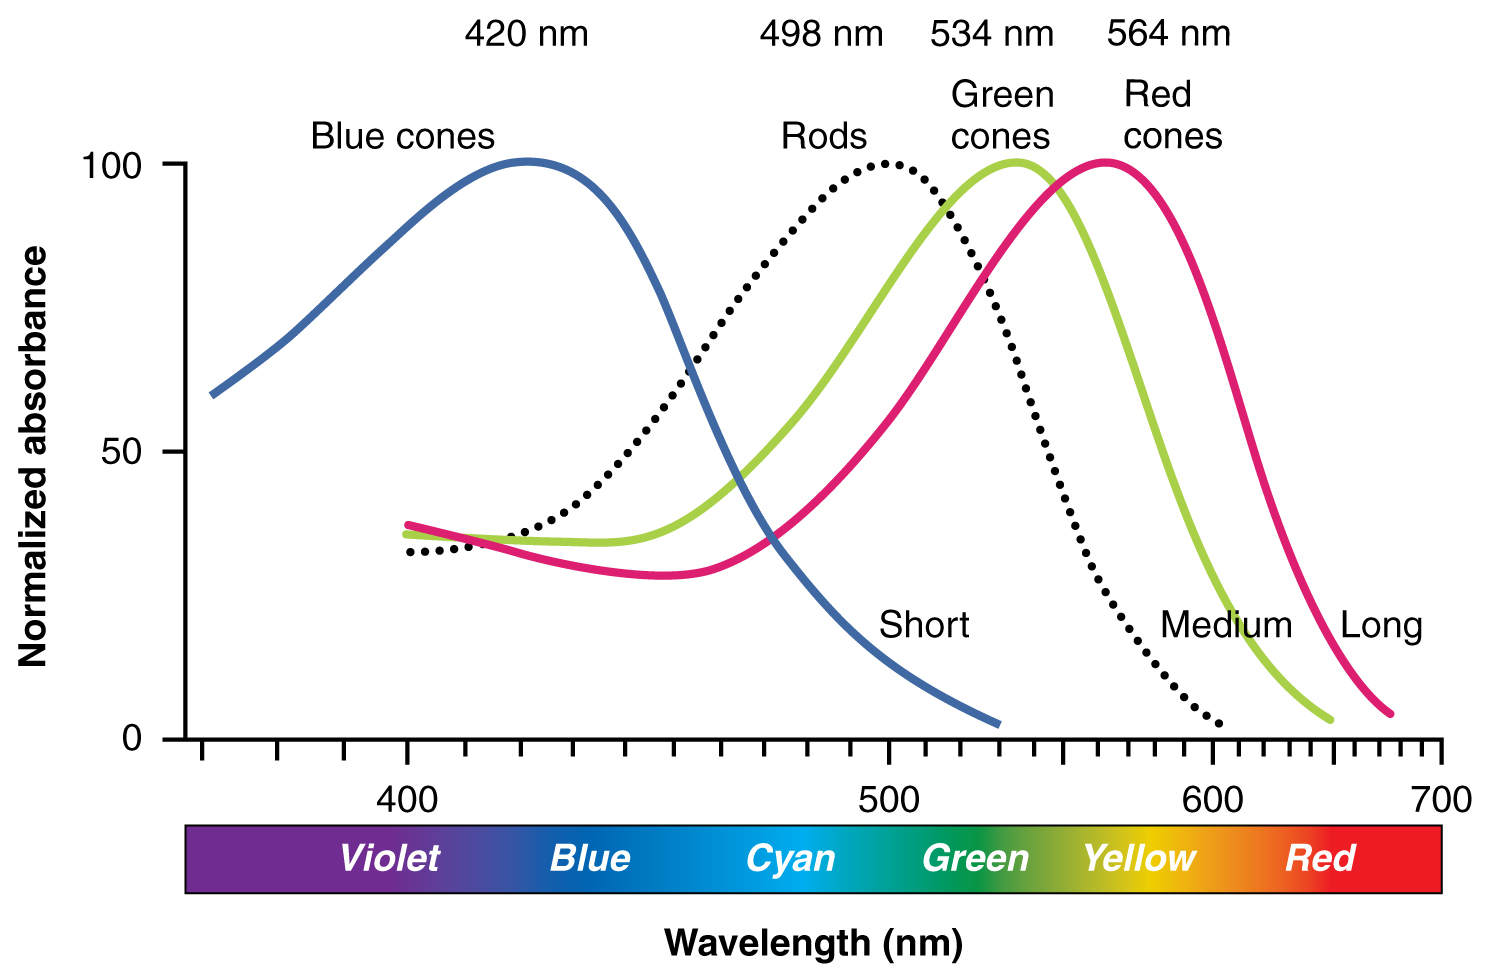
\includegraphics[width=10cm]{\imgpath/colour_sensitivity.jpg}
      % \mycaption{Frequency sensitivity of photoreceptors in they eye}
              % {Wavelength responsiveness of the different photoreceptors in the
               % eye. S, M, and L are short, medium, and long cones, compared to
               % R --- rods. Taken from~\cite{bowmaker_visual_1980}}
  % \end{center}
% \end{figure}

The current state of the art in image understanding systems are
Convolutional Neural Networks (CNNs). These are a learned model that
cascades many convolutional filters serially in layers, separated by
nonlinearities.
They are seemingly inspired by the visual cortex in the way that they are
hierarchically connected, progressively compressing the information into a
richer representation.

\autoref{fig:ch1:cnn_arch} shows an example CNN
architecture, the famous AlexNet \cite{krizhevsky_imagenet_2012}. Inputs are resized to a
manageable size, in this case, $224\x 224$ pixels. Multiple convolutional
filters of size $11\x 11$ are convolved over this input to give $96$ output
\emph{channels} (or \emph{activation maps}). In the figure, these are split onto two
graphics cards or GPUs for memory purposes. These are then passed through a
pointwise nonlinear function, or \emph{nonlinearity}.
The activations are pooled (a form of downsampling) and convolved with more
filters to give $256$ new channels at the second stage. This is repeated 3 more
times until the $13\x 13$ output with $256$ channels is unravelled and passed
through a fully connected neural network to classify the image as one of $1000$
possible classes.

CNNs have garnered lots of attention since 2012 when the previously mentioned AlexNet
nearly halved the top-5 classification error rate (from $26\%$ to $16\%$)
in the ImageNet Large Scale Visual Recognition Competition (ILSVRC)
\cite{russakovsky_imagenet_2014}\footnote{The previous state of
the art classifiers had been built by combining keypoint extractors like
SIFT\cite{lowe_distinctive_2004} and HOG\cite{dalal_histograms_2005} with
classifiers such as Support Vector Machines\cite{cortes_support-vector_1995} and
Fisher Vectors\cite{sanchez_image_2013}, for example \cite{sanchez_high-dimensional_2011}.}.
In the years since, the complexity of CNNs has grown significantly. AlexNet had
only 5 convolutional layers, whereas the 2015 ILSVRC winner ResNet \cite{he_deep_2016}
achieved 3.57\% top-5 error with 151 convolutional layers (and had some
experiments with 1000 layer networks).

\begin{figure}
  \centering
    % \includegraphics[width=\textwidth]{\imgpath/dtcwt_gain}
    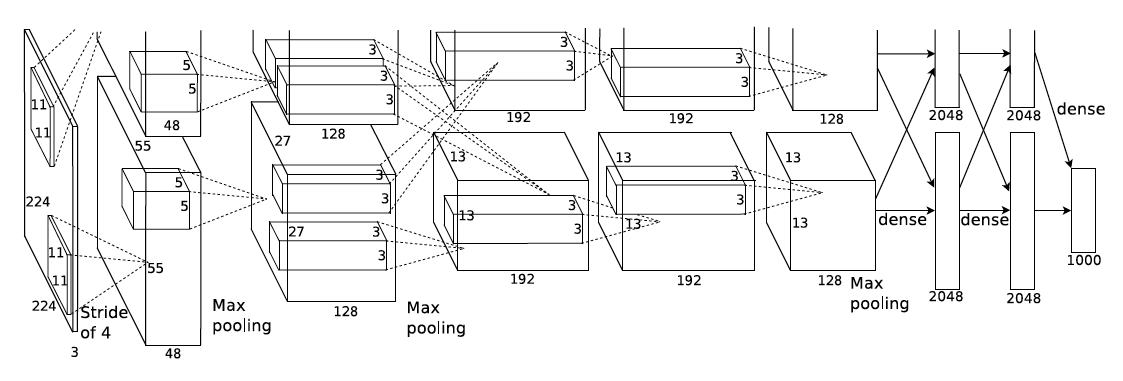
\includegraphics[width=\textwidth]{\imgpath/alexnet.png}
    \mycaption{Convolutional Architecture example}{The previous layer's activations are
    combined with a learned convolutional filter.
    Note that while the activation maps are 3-D arrays, the convolution is only
    a 2-D operation. This means the filters have the same number of channels as
    the input and produce only one output channel. Multiple channels are made by
    convolving with multiple filters. Not shown here are the nonlinearities that
    happen in between convolution operations. Image taken from \cite{krizhevsky_imagenet_2012}.}
    \label{fig:ch1:cnn_arch}
  \end{figure}

\section{Motivation}\label{sec:ch1:motivation}
\begin{figure}
  \centering
  \subfloat[conv1 filters]{
  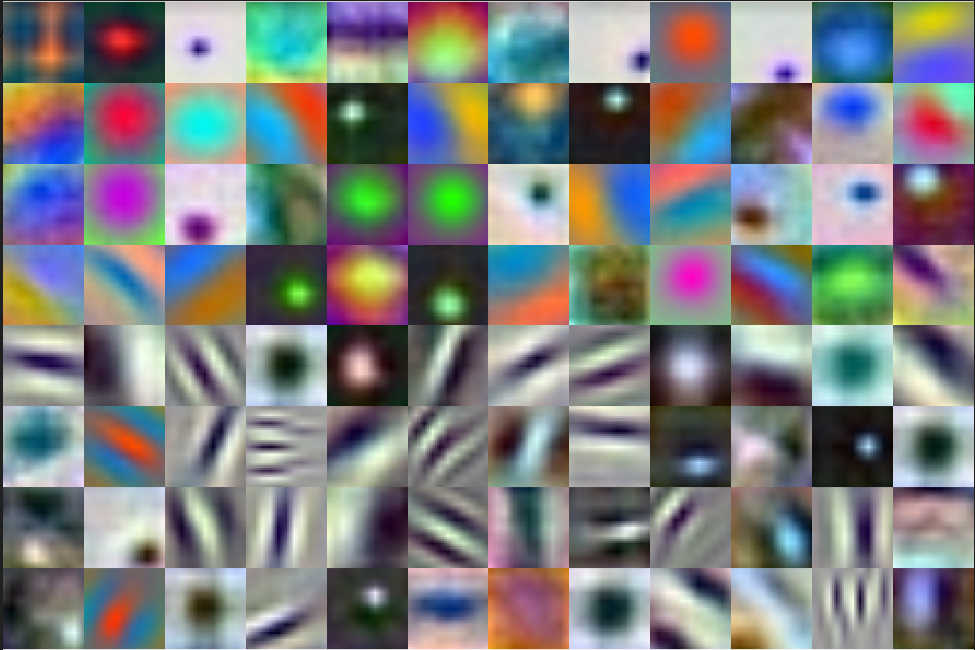
\includegraphics[width=0.6\textwidth]{\imgpath/alexfilters.png}
  \label{fig:ch1:alex_filt}
  }\\
  \subfloat[conv1 activations]{
  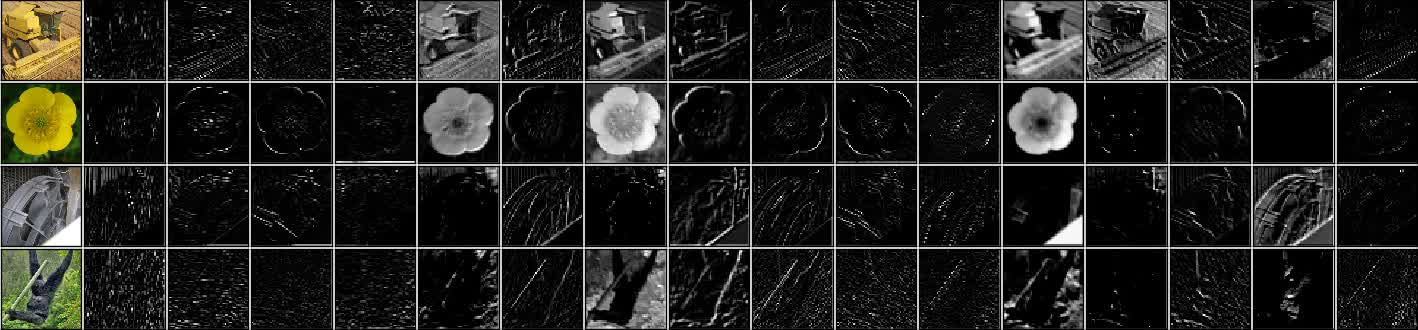
\includegraphics[width=\textwidth]{\imgpath/out1.jpg}
  \label{fig:ch1:alex_conv1}
  }\\
  \subfloat[conv2 activations]{
  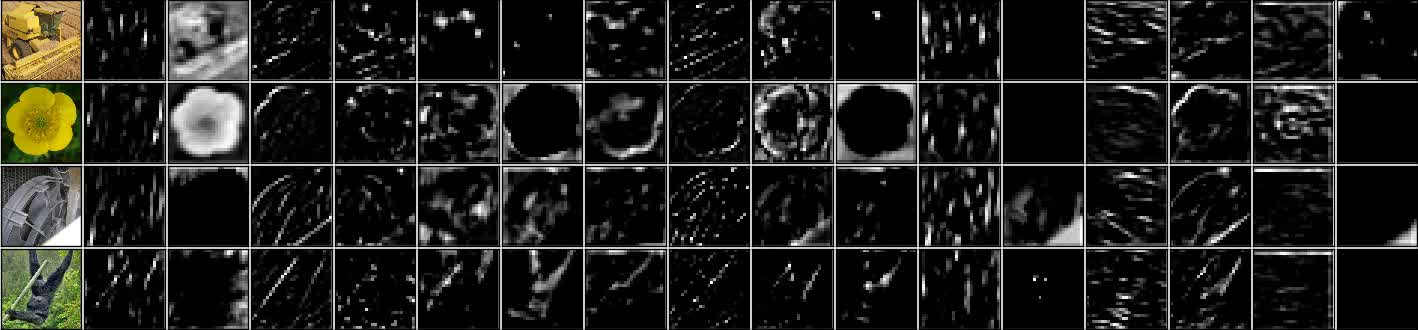
\includegraphics[width=\textwidth]{\imgpath/out2.jpg}
  \label{fig:ch1:alex_conv2}
  }\\
  \subfloat[conv3 activations]{
  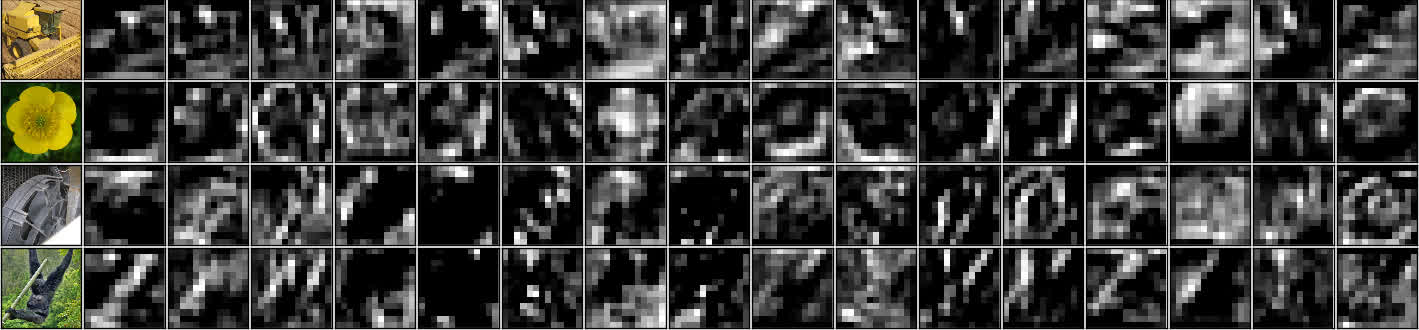
\includegraphics[width=\textwidth]{\imgpath/out3.jpg}
  \label{fig:ch1:alex_conv3}
  }
  \mycaption{Example first layer filters and the first three
  layer's outputs}{\subref{fig:ch1:alex_filt} The $11\x 11$ filters for the
  first stage of AlexNet. Of the 96 filters, 48 were learned on one GPU and
  another 48 on another GPU. Interestingly, one GPU has learned mostly
  lowpass/colour filters and the other has learned oriented bandpass
  filters. \subref{fig:ch1:alex_conv1} - \subref{fig:ch1:alex_conv3} Randomly
  chosen activations from the output of the first, second and third convolutional
  layers of AlexNet (see \autoref{fig:ch1:cnn_arch}) with negative values set to 0.
  Filters and activation images taken from supplementary material of
    \cite{krizhevsky_imagenet_2012}.}
  \label{fig:ch1:alexnet_filters}
\end{figure}

Despite their success, CNNs are often criticized for being \emph{black-box}
methods. You can view the first layer of filters
quite easily (see \autoref{fig:ch1:alex_filt}) as they exist in RGB
space, but beyond that things get trickier as the filters have a third, \emph{channel}
dimension, typically much larger than the two spatial dimensions. Additionally,
it is not clear what the input channels themselves correspond to. For illustration
purposes, we have also shown some example activations from the first three
convolutional layers for AlexNet in
\autoref{fig:ch1:alexnet_filters}\subref{fig:ch1:alex_conv1}-\subref{fig:ch1:alex_conv3}\footnote{These activations are
taken after a specific nonlinearity that sets negative values to 0, hence the
large black regions.}. For the conv1 activations in
\autoref{fig:ch1:alex_conv1}, we can accurately guess that some of the first layer
channels are responding to edges or colour information, but as we go deeper to
conv2 and conv3, it becomes less and less clear what each activation is
responding to.

This has started to become a problem, and while we are happy to trust modern
CNNs for isolated tasks, we are less likely to be comfortable with them driving
cars through crowded cities, or making executive decisions that affect people
directly. In a commonly used contrived example, it is not hard to imagine a deep
network that could be used to assess whether giving a bank loan to an applicant
is a safe investment. Trusting a black box solution is deeply unsatisfactory in
this situation. Not only from the customer's perspective, who, if declined, has
the right to know why \cite{goodman_european_2016}, but
also from the bank's --- before lending large sums of money, most banks
would like to know why the network has given the all clear. `It has worked well
before' is a poor rule to live by.

Aside from their lack of interpretability, it often takes a long time and a lot of
effort to train state-of-the-art CNNs. Typical networks that have won ILSVRC
since 2012 have had roughly 100 million parameters and take up to a week to train. This
is optimistic and assumes that you already know the necessary optimization or
architecture hyperparameters, which you often have to find out by trial and error.
In a conversation the author had with Yann LeCun, the attributed father of
CNNs, at a Computer Vision Summer School (ICVSS 2016), LeCun highlighted this problem
himself:
\begin{quote}
  There are certain recipes (for building CNNs) that work and certain recipes
  that don't, and we don't know why.
\end{quote}

Considering the recent success of CNNs, it is becoming more and more
important to understand \emph{how} and \emph{what} a network learns, so we can
interrogate what in the input has contributed to it making its classification or regression choice.
Without this information, the use of these incredibly powerful tools could be
restricted to research and proprietary applications.

\section{Approach}
The structure of convolutional layers is fairly crude in terms of signal
processing - arbitrary taps of an FIR filter are learned typically via
stochastic gradient descent from random starting states to minimize either a
mean-squared error or cross-entropy loss.

This leads us to ask a motivating question:
%
\begin{quote}
  Is it possible to learn convolutional filters as combinations of basis
  functions rather than individual filter taps?
\end{quote}

In achieving this, it is important to find ways to have an adequate
richness of filtering while reducing the number of parameters needed to specify resulting
filters. We want to contract the space of learning to a subspace or manifold that
is more useful. In much the same way, the convolutional layer in a CNN is a restricted
version of a fully connected layer in a multi-layer perceptron, yet adding this
restriction allowed us to train more powerful networks.

\begin{quote}
The intuition that we explore in this thesis is that \emph{complex wavelets} are
good basis functions for filtering in CNNs.
\end{quote}

\subsection{Why Complex Wavelets?}
Most modern approaches to CNNs are framed entirely in the spatial domain; our
choice of complex wavelets as the basis function to explore comes from the
deeper intuition that it may be helpful to rethink about CNNs in the
\emph{frequency domain}.  Historically, the frequency domain has been an
excellent space for solving many signal processing problems such as noise
removal, filter design, edge detection and data compression. We believe it may prove to
have advantages for CNNs too (beyond just an efficient space to do convolution
in).

The Fourier transform, which uses complex sinusoids as
its basis function, is perhaps the most ubiquitous tool to use for frequency
domain analysis. The problem with these complex sinusoids is that they have
\emph{infinite} support. This means that small changes in one part of an image
affect every Fourier coefficient. Additionally, they are not stable to small
deformations, as small changes can produce unbounded changes in the representation
\cite{mallat_group_2012}.

The common remedy to this problem is to use the localized, and more
stable, short-time Fourier transform (STFT). The STFT (or the Gabor transform)
is a natural extension of the Fourier transform, windowing the complex sinusoids
with a Gaussian (or similar) function. The STFT has the undesirable property that all
frequencies are sampled with the same resolution. A close relative of the STFT is the
continuous wavelet transform (CWT). The shorter duration of the wavelet basis
functions as the frequency increases means that their time resolving power
improves with centre-frequency.
Another commonly used
wavelet transform is the discrete wavelet transform (or the DWT) often favoured over
the CWT because of its speed of computation. It can use many
different finite support basis functions, all with different frequency
localization properties, but it is usually limited to using real filters. As such, it
suffers from many problems such as shift-dependence and lack of directionality in
two dimensions (2-D). These problems can be remedied by using the slower CWT with complex basis
functions, but we choose instead to use the dual-tree complex wavelet transform,
or $\DTCWT$ \cite{selesnick_dual-tree_2005} with q-shift filters \cite{kingsbury_complex_2001}.

The $\DTCWT$ allows for complex basis functions that have shift-invariance and
directionality, while being fast to implement like the DWT (in 2-D it can be thought of as the
application of 4 DWTs in parallel). It is also more easily invertible than the
CWT, forming a tight frame \cite{kovacevic_introduction_2008}, which we believe
may prove to be a very important property for visualizing what a
CNN is responding to.

We revisit the properties of the Fourier transform, STFT, CWT, DWT and $\DTCWT$
and expand on the properties behind our choice of basis functions
in the literature review \autoref{sec:ch2:fourier}.

On top of the intuition that the wavelet domain is a good space in which to frame CNNs,
there are some experimental motivating factors too. Firstly, the wavelet
transform has had much success in image and video compression, particularly for
JPEG2000 \cite{taubman_jpeg2000_2013}. Good compression performance implies an ability of
the basis functions to represent the input data sparsely (as seems to happen in
the brain). Secondly, the filters from the first layer of AlexNet
(\autoref{fig:ch1:alexnet_filters}) look like oriented wavelets. Given that
there was no prior placed on the filters to make them have this similarity to
wavelets, this result is noteworthy. And finally, the aforementioned work of
Hubel and Wiesel suggests that the early layers of the visual system act like a
Gabor transform.

These experimental observations imply that complex wavelets would do well in
replacing the first layer of a CNN, but we would aslo like to find out if they can be used
at deeper layers. Their well-understood and well-defined behaviour would help us
to answer the above \emph{how} and \emph{why} questions. Additionally, they
allow us to enforce a certain amount of smoothness and near orthogonality;
smoothness seems to be important to avoid sensitivity to adversarial or spoofing
attacks \cite{szegedy_intriguing_2014} and near orthogonality allows you to
cover a large space with fewer coefficients.

But first, we must find out \emph{if} it is possible to get the same or nearly the same
performance by using wavelets as the building blocks for CNNs, and this is the
core goal of this thesis.

\section{Method}
\subsection{ScatterNets}
To explore the uses of complex wavelets in CNNs, we begin by looking at one of the most
popular current uses of wavelets in image recognition tasks, the
Scattering Transform.

The Scattering Transform, or the \emph{ScatterNet}, was introduced in \cite{mallat_group_2012,
bruna_invariant_2013} at the same time as AlexNet. It is a non-black-box
network that can be thought of as a restricted complex-valued CNN
\cite{bruna_mathematical_2015}. Unlike a CNN, it has predefined
convolutional kernels, set to complex wavelet (and scaling) functions and uses
the complex magnitude as its nonlinearity. Due to
its well-defined structure, it can be analyzed and bounds on its stability to
shifts, noise and deformations are found in \cite{mallat_group_2012}.
%
% This is a promising start to addressing the problems of CNNs as using
% predefined, general filters helps us answer \emph{how} a CNN is
% learning, although the \emph{what} is still somewhat unclear.

For a simple task like identifying small handwritten digits,
the variabilities in the data are simple and small and the ScatterNet can easily
reduce the problem into a space which a Gaussian Support Vector Machine (or SVM
\cite{cortes_support-vector_1995}) can easily solve
\cite{bruna_invariant_2013}. For a more complex task like identifying real-world
objects, the ScatterNet can somewhat reduce the variabilities and get good
results with an SVM, but there is a significant performance gap between this and
what a CNN can achieve. For example, in \cite{oyallon_deep_2015} a second-order
ScatterNet can achieve $82.3\%$ top-1 classification accuracy on CIFAR-10, a
commonly used dataset, whereas modern CNNs such as \cite{he_deep_2016} can
achieve $93.4\%$.

\subsection{Learnable ScatterNets}
To start to address the performance gap between ScatterNet front ends and CNNs
we first investigate the properties of current ScatterNets. Inspired by the
visualization work of \citeauthor{zeiler_visualizing_2014}
\cite{zeiler_visualizing_2014} we build a DeScatterNet. The DeScatterNet
leverages the perfect reconstruction properties of the $\DTCWT$ and allows us to
investigate what in the input image the ScatterNet is responding to.

The DeScatterNet shows that the ScatterNet may be limiting itself by not
combining the filtering of different wavelet orientations (it does not mix the
channels as a CNN does). Inspired by the work of \cite{qiu_dcfnet:_2018}, we
propose the learnable ScatterNet, which includes this mixing while keeping the
desirable properties of the ScatterNet.

The learnable ScatterNet can be thought of as using the scattering outputs as
the \emph{basis functions}\footnote{Although they are not true basis functions
as they are the combination of a complex wavelet with a modulus nonlinearity,
and are thus data-dependent.} for our convolutional layers. We show that this
improves greatly on the ScatterNet design, and under certain constraints can
improve on the performance of CNNs too.

\subsection{Wavelet Domain Filtering}
We find that the complex modulus of the ScatterNet design to be useful for some
operations in a CNN, but it has a demodulating effect on the frequency energy
(all the outputs have significantly more energy in lower frequencies). This
limits repeated application of it as the demodulating effect compounds.

We develop a system that does not use the complex modulus; instead, it
learns \emph{complex} gains in the wavelet domain.
Rather than mixing subbands together, we keep them independent and only learn to
mix across the channel dimension. This is important, as it allows us to then use the inverse
$\DTCWT$ to return to the pixel domain. The shift-invariant properties of the $\DTCWT$ mean the
reconstructed outputs are (mostly) free from aliasing effects, despite much of
the processing being carried out at significantly reduced sample rates in the
wavelet domain.

We show that our layer can be used alongside regular convolutional
layers. I.e., it becomes possible to `step' into the wavelet domain to do
wavelet filtering for one layer, before `stepping' back into the pixel domain to
do pixel filtering for the next layer.

\section{Thesis Layout and Contributions to Knowledge}
This thesis has one literature review chapter and four novel-work chapters:
\begin{itemize}
\item
  \hyperref[ch:litreview]{Chapter~\ref*{ch:litreview}}
  explores some of the background necessary for starting
  to develop image understanding models. In particular, it covers the
  inspiration for CNNs and the workings of CNNs themselves, as well as covering
  the basics of wavelets and ScatterNets.
\item
  \Autoref{Chapter}{ch:dtcwt_scat} proposes a change to the core of the ScatterNet. In
  addition to performance issues with ScatterNets, they are slow and both
  memory-intensive and compute-intensive to calculate. This in itself is enough of an
  issue to make it unlikely that they would be used as part of deep networks. To
  overcome this, we change the computation to use the $\DTCWT$
  \cite{selesnick_dual-tree_2005} instead of Morlet wavelets, achieving a 20 to
  30 times speed-up while achieving a small improvement in classification performance.
\item
  \Autoref{Chapter}{ch:visualizing} describes our \emph{DeScatterNet}, a tool used to
  interrogate the structure of ScatterNets. We also perform tests to determine
  the usefulness of the different scattered outputs finding that many of them
  are not useful for image classification.
\item
  \Autoref{Chapter}{ch:invariant} describes the \emph{Learnable ScatterNet} we have developed to
  address some of the issues found from the interrogation in
  \autoref{ch:visualizing}. We find that a learnable ScatterNet layer performs
  better than a regular ScatterNet, and can improve on the performance of a CNN
  if used instead of pooling layers. We also find that scattering works well not
  just on RGB images, but can also be useful when used after one layer of
  learning.
\item
  In \autoref{ch:freqlearn}, we step away from ScatterNets and present the
  \emph{Wavelet Gain Layer}. The gain layer uses
  the wavelet space as a latent space to learn representations. We find possible
  nonlinearities and describe how to learn in both the pixel and wavelet domain.
  This work showed that there may well be benefits to learning in the wavelet
  domain for earlier layers of CNNs, but we have not yet found advantages to
  using the wavelet gain layer for deeper layers.
\end{itemize}

\subsection{Contributions and Publications}
The key contributions of this thesis are:

\begin{itemize}
  \item Software for wavelets and $\DTCWT$ based ScatterNet (described in \autoref{ch:dtcwt_scat})
    and publicly available at \cite{cotter_pytorch_2018}.
  \item ScatterNet analysis and visualizations (described in
    \autoref{ch:visualizing}). This chapter expands on the paper we presented at MLSP2017
    \cite{cotter_visualizing_2017}.
  \item Invariant Layer/Learnable ScatterNet (described in \autoref{ch:invariant})). This chapter expands
    on the paper accepted at ICIP2019 \cite{cotter_learnable_2019}. Software
    available at \cite{cotter_learnable_2019-1}.
  \item Learning convolutions in the wavelet domain (described in
    \autoref{ch:freqlearn}). We have published preliminary results on this work
    to arXiv \cite{cotter_deep_2018} but have expanded on this paper in the
    chapter. Software available at \cite{cotter_dtcwt_2018}.
\end{itemize}

\subsection{Related Research}
Readers may also be interested in the theses \cite{singh_scatternet_2018} and
\cite{oyallon_analyzing_2017}.

In \cite{singh_scatternet_2018}
\citeauthor{singh_scatternet_2018} looks at using the ScatterNet as a fixed
front end and combining it with well-known machine learning methods such as
SVMs, Autoencoders and Restricted Boltzmann Machines. By combining frameworks in
a defined way he creates unsupervised feature extractors which can then be used
with simple classifiers. Some relevant papers that makeup this thesis are \cite{singh_multi-resolution_2016,
singh_scatternet_2017, singh_generative_2018}. In
\cite{singh_multi-resolution_2016} Singh shows
that the $\DTCWT$-ScatterNet outperforms a Morlet-ScatterNet when used as a front end for
an SVM, which is similar to the work we do in \autoref{ch:dtcwt_scat} where we
show the $\DTCWT$-ScatterNet outperforms a Morlet-ScatterNet when used as a
front end for CNNs. He then expands on this work by testing other backends in
\cite{singh_scatternet_2017, singh_generative_2018}.

In \cite{oyallon_analyzing_2017}
\citeauthor{oyallon_analyzing_2017} looks at ScatterNets as front ends to
deeper learning systems, such as CNNs. Some relevant papers that makeup Oyallon's thesis are
\cite{oyallon_deep_2015, oyallon_scaling_2017, oyallon_hybrid_2017}. \cite{oyallon_scaling_2017, oyallon_hybrid_2017}
are particularly relevant as he uses a ScatterNet as a feature extractor for a
CNN. We do similar research in \autoref{ch:invariant}, but allow for
learned weights in the ScatterNet in our design.

% \section{Related Work}\label{sec:ch5:related}

There have been several similar works that look into designing new convolutional
layers by separating them into two stages --- a first stage that performs a
non-standard filtering process, and a second stage that combines the first stage
into single activations. The inception layer 
\cite{szegedy_rethinking_2015} by \citeauthor*{szegedy_rethinking_2015} does this by filtering with different
kernel sizes in the first stage, and then combining with a $1\x 1$ convolution
in the second stage. \citeauthor*{ioannou_training_2015} also do something similar by making
a first stage with horizontal and vertical filters, and then combining in the
second stage again with a $1\x 1$ convolution\cite{ioannou_training_2015}. But perhaps the most similar
works are those that use a first stage with fixed filters, combining them in a
learned way in the second stage. Of particular note are:
\begin{itemize}
\item 
\citetitle{juefei-xu_local_2016} \cite{juefei-xu_local_2016}. This paper builds a
first stage with a small $3\x 3$ kernel filled with zeros, and randomly insert
$\pm 1$ in several locations, keeping a set sparsity level. This builds a very
crude spatial differentiator in random directions. The output of the first stage
is then passed through a sigmoid nonlinearity before being mixed with a $1\x 1$
convolution. The imposed structure on the first stage was found to be a good
regularizer and prevented overfitting, and the combination of the mixing in the
second layer allowed for a powerful and expressive layer, with performance near
that of a regular CNN layer.

\item
``DCFNet: Deep Neural Network with Decomposed Convolutional Filters"
\cite{qiu_dcfnet:_2018}. This paper decomposes convolutional filters as linear
combinations of Fourier Bessel and random bases.  The first stage projects the
inputs onto the chosen basis, and the second stage learns how to mix these
projections with a $1\x 1$ convolution. Unlike \cite{juefei-xu_local_2016} this
layer is purely linear. The supposed advantage being that the
basis can be truncated to save parameters and make the input less susceptible to
high frequency variations. The work found that this layer had marginal benefits
over regular CNN layers in classification, but had improved stability to noisy
inputs. 

\end{itemize}

\section{Recap of Useful Terms}\label{sec:ch5:background}

\subsection{Convolutional Layers}\label{sec:ch5:conv}

Let the output of a CNN at layer $l$ be 
$ \cnnlact{x}{l}{c}{\xy}, \quad c\in \{0, \ldots C_l-1\}, \xy \in \reals[2]$
where $c$ indexes the channel dimension, and $\xy$ is a vector of coordinates
for the spatial position. Of course, $\xy$ is typically sampled on a grid, but
we keep it continuous to more easily differentiate between the spatial and
channel dimensions. Recall from \eqref{eq:ch2:conv4} and \eqref{eq:ch2:conv4a} that
a convolutional layer in a standard CNN is defined by the two operations:
%
\begin{eqnarray} 
  \cnnlact{y}{l+1}{f}{\xy} &=& \sum_{c=0}^{C_l - 1}  x^{(l)}(c,\xy) \conv h^{(l)}_{f}(c, \xy)
    \label{eq:ch5:conv}\\
    \cnnlact{x}{l+1}{f}{\xy} & = & \sigma \left( \cnnlact{y}{l+1}{f}{\xy} \right) \label{eq:ch5:nonlin}
\end{eqnarray}

where $\cnnfilt{l}{f}{c}{\xy}$ is the $f$th filter of the $l$th layer with $C_l$
different point spread functions, and $f \in \{0, \ldots, C_{l+1}-1 \}$. $\sigma$ is a nonlinearity 
such as the ReLU, possibly combined with scaling such as batch normalization. The convolution
is done independently for each $c$ in the $C_l$ channels and the resulting outputs are
summed together to give one activation map. 

\subsection{Wavelet Transforms}\label{sec:ch5:wavelets}
Recall from \eqref{eq:ch2:wave2} that:
\begin{equation}
  \mathcal{W}x(c, \xy) = \left\{x(c, \xy) \ast \phitd_J(\xy),\ x(c, \xy) \ast \psitd_{\lambda}(\xy) \right\}_{\lambda} \label{eq:ch5:wave2}
\end{equation}
Where $\psitd_\lambda$ is a mother wavelet dilated by $2^j,\ 1 \leq j \leq J$ and rotated by
$\theta = \frac{\pi + 2k\pi}{12},\ 0\leq k < 6$:
%
\begin{equation}
  \psi_{j, \theta}(\xy) = 2^{-j}\psi \left(2^{-j} r_{-\theta} \xy\right)
\end{equation}
Define the set of all possible $\lambda$s as $\Lambda$ whose size is $|\Lambda | = JK$.
%
\subsection{Scattering Transforms}\label{sec:ch5:scatter}
As the real and imaginary parts of complex wavelets are in quadrature with
each other, taking the modulus of the resulting transformed coefficients removes
the high frequency oscillations of the output signal while preserving the energy
of the coefficients over the frequency band covered by $\psi_\lambda$. This is
crucial to ensure that the scattering energy is concentrated towards
zero-frequency as the scattering order increases, allowing sub-sampling.
% We experimentally show in \autoref{sec:??} that it plays a vital role in the
%classification process. 
We define the wavelet modulus propagator to be:
%
\begin{equation}
  \label{eq:ch5:wave_mod}
\widetilde{\mathcal{W}}x(c, \xy) = \left\{ x(c, \xy) \conv \phi_{J}(\xy),\ |x(c, \xy) \conv \psi_\lambda (\xy) | \right\}_{\lambda \in \Lambda} 
\end{equation}
The modulus terms are called $U[\lambda] x = \lvert x \conv \psi_\lambda \rvert$, and the scattering terms
are $S[\lambda] x = U[\lambda]x \conv \phi_J (\xy)$.

\section{The Scattering Transform} \label{sec:ch4:scatternet}
While we have introduced the scattering transform before, we clarify the format
we use for this chapter's analysis.

We use the $\DTCWT$ based ScatterNet introduced in the previous chapter --
\autoref{alg:ch3:dtcwt_scat} as a front end, with $K=6$ orientations, $J=2$
scales and $M=2$ orders.

Consider a single-channel input signal $x(\xy)$, $\xy \in \reals[2]$.
The zeroth-order scatter coefficient is the lowpass output of a $J$
level filter bank:
%
\begin{equation}
  S_0x(\xy) \definedas x(\xy) \conv \phi_J(\xy)
\end{equation}
%
This is approximately invariant to translations of up to $2^J$ pixels\footnote{From here on,
we drop the $\xy$ notation when indexing $x$, for clarity.}. In exchange for
gaining invariance, the $S_0$ coefficients have lost information
(contained in the rest of the frequency space). The remaining energy of $x$ is
contained within the first-order \emph{wavelet} coefficients:
\begin{equation}
  W_1x(\lambda_1, \xy) \definedas x \conv \psi_{\lambda_1}
\end{equation}
for $\lambda_1 = (j_1, \theta_1)$, $j_1\in\{1, 2\}, \theta_1 = \frac{\pi +
2k\pi}{12}$ with $k \in \{0, 1, \ldots 5\}$.

Taking the magnitude of $W_1$ gives us the first-order \emph{propagated}
signals:
\begin{equation}
  U_1x(\lambda_1, \xy) \definedas |x \conv \psi_{\lambda_1}|
    = \sqrt{(x \conv \psi^r_{\lambda_1})^2 + (x \conv \psi^i_{\lambda_1})^2}
\end{equation}
The first-order scattering coefficient make $U_1$ invariant up to
the coarsest scale $J$ by averaging it:
\begin{equation}
  S_1x(\lambda_1, \xy) \definedas |x \conv \psi_{\lambda_1}| \conv \phi_J
\end{equation}
This has $KJ = 6\x 2 = 12$ output channels for each input channel. Later in this
chapter we will want to distinguish between the first and second scale
coefficients of the $S_1$ terms, which we will do by moving the $j$ index
to a superscript. I.e., $S_1^1$ and $S_1^2$ refer to the set of 6 $S_1$ terms
at the first and second scales.

The second-order scattering coefficients are defined only on paths of
decreasing frequency (i.e. $J_2 < J_{1}$) \cite{bruna_invariant_2013}
\begin{equation}
  S_2x(\lambda_1, \lambda_2, \xy) \definedas |U_1x \conv \psi_{\lambda_2}| \conv \phi_J \label{eq:ch4:s2}
\end{equation}
Previous work shows that for natural images we get diminishing returns after
$m=2$. Our output is then a stack of these 3 outputs:
\begin{equation}
  Sx = \{S_0x, S_1x, S_2x\}
\end{equation}
with $1+12+36=49$ channels per input channel.

\subsection{Scattering Colour Images}\label{sec:ch4:colour}
A wavelet transform like the $\DTCWT$ accepts single-channel input yet we
often work on RGB images. This leaves us with a choice. We can either:
\begin{enumerate}
  \item Apply the wavelet transform (and the subsequent scattering operations)
    on each channel independently. This would triple the output size to $3C$.
  \item Define a frequency threshold below which we keep colour information, and
    above which, we combine the three channels.
\end{enumerate}
The second option uses the well known fact that the human eye is far less sensitive
to higher spatial frequencies in colour channels than in luminance channels.
This also fits in with the first layer filters seen in the well known
Convolutional Neural Network, AlexNet. Roughly one half of the filters were low
frequency colour `blobs', while the other half were higher frequency, greyscale,
oriented wavelets.

For this reason, we choose the second option for the
architecture described in this chapter. We keep the 3 colour
channels in our $S_0$ coefficients but work only on greyscale for high orders
(the $S_0$ coefficients are the lowpass bands of a J-scale wavelet transform, so
we have effectively chosen a colour cut-off frequency of $2^{-J} \frac{f_s}{2}$).

We combine the three channels by modifying our magnitude operation from \eqref{eq:ch3:magbias}
to now be:
\begin{equation}\label{eq:ch4:colour_mag}
 r_s = \sqrt{x_r^2 + y_r^2 + x_g^2 + y_g^2 + x_b^2 + y_b^2 + b^2} - b
\end{equation}
Where $x_r, x_g, x_b$ are the real parts of the wavelet response for the red,
green and blue channels, and $y$ is the corresponding imaginary part. This only
affects the $S_1$ coefficients and the $S_2$ coefficients then are calculated
as per \eqref{eq:ch4:s2}.

An alternative to \eqref{eq:ch4:colour_mag} is to combine the colours
\emph{before} scattering into a luminance channel. However, we choose to use \eqref{eq:ch4:colour_mag}
instead as this has the ability to detect colour edges with constant luminance.

With $J=2$ the resulting scattering output now has $3 + 12 + 36 = 51$ channels at $1/16$ the
spatial input size.

\section{The Inverse Scatter Network}\label{sec:ch4:descatternet}
\begin{figure}[t]
  \centering
  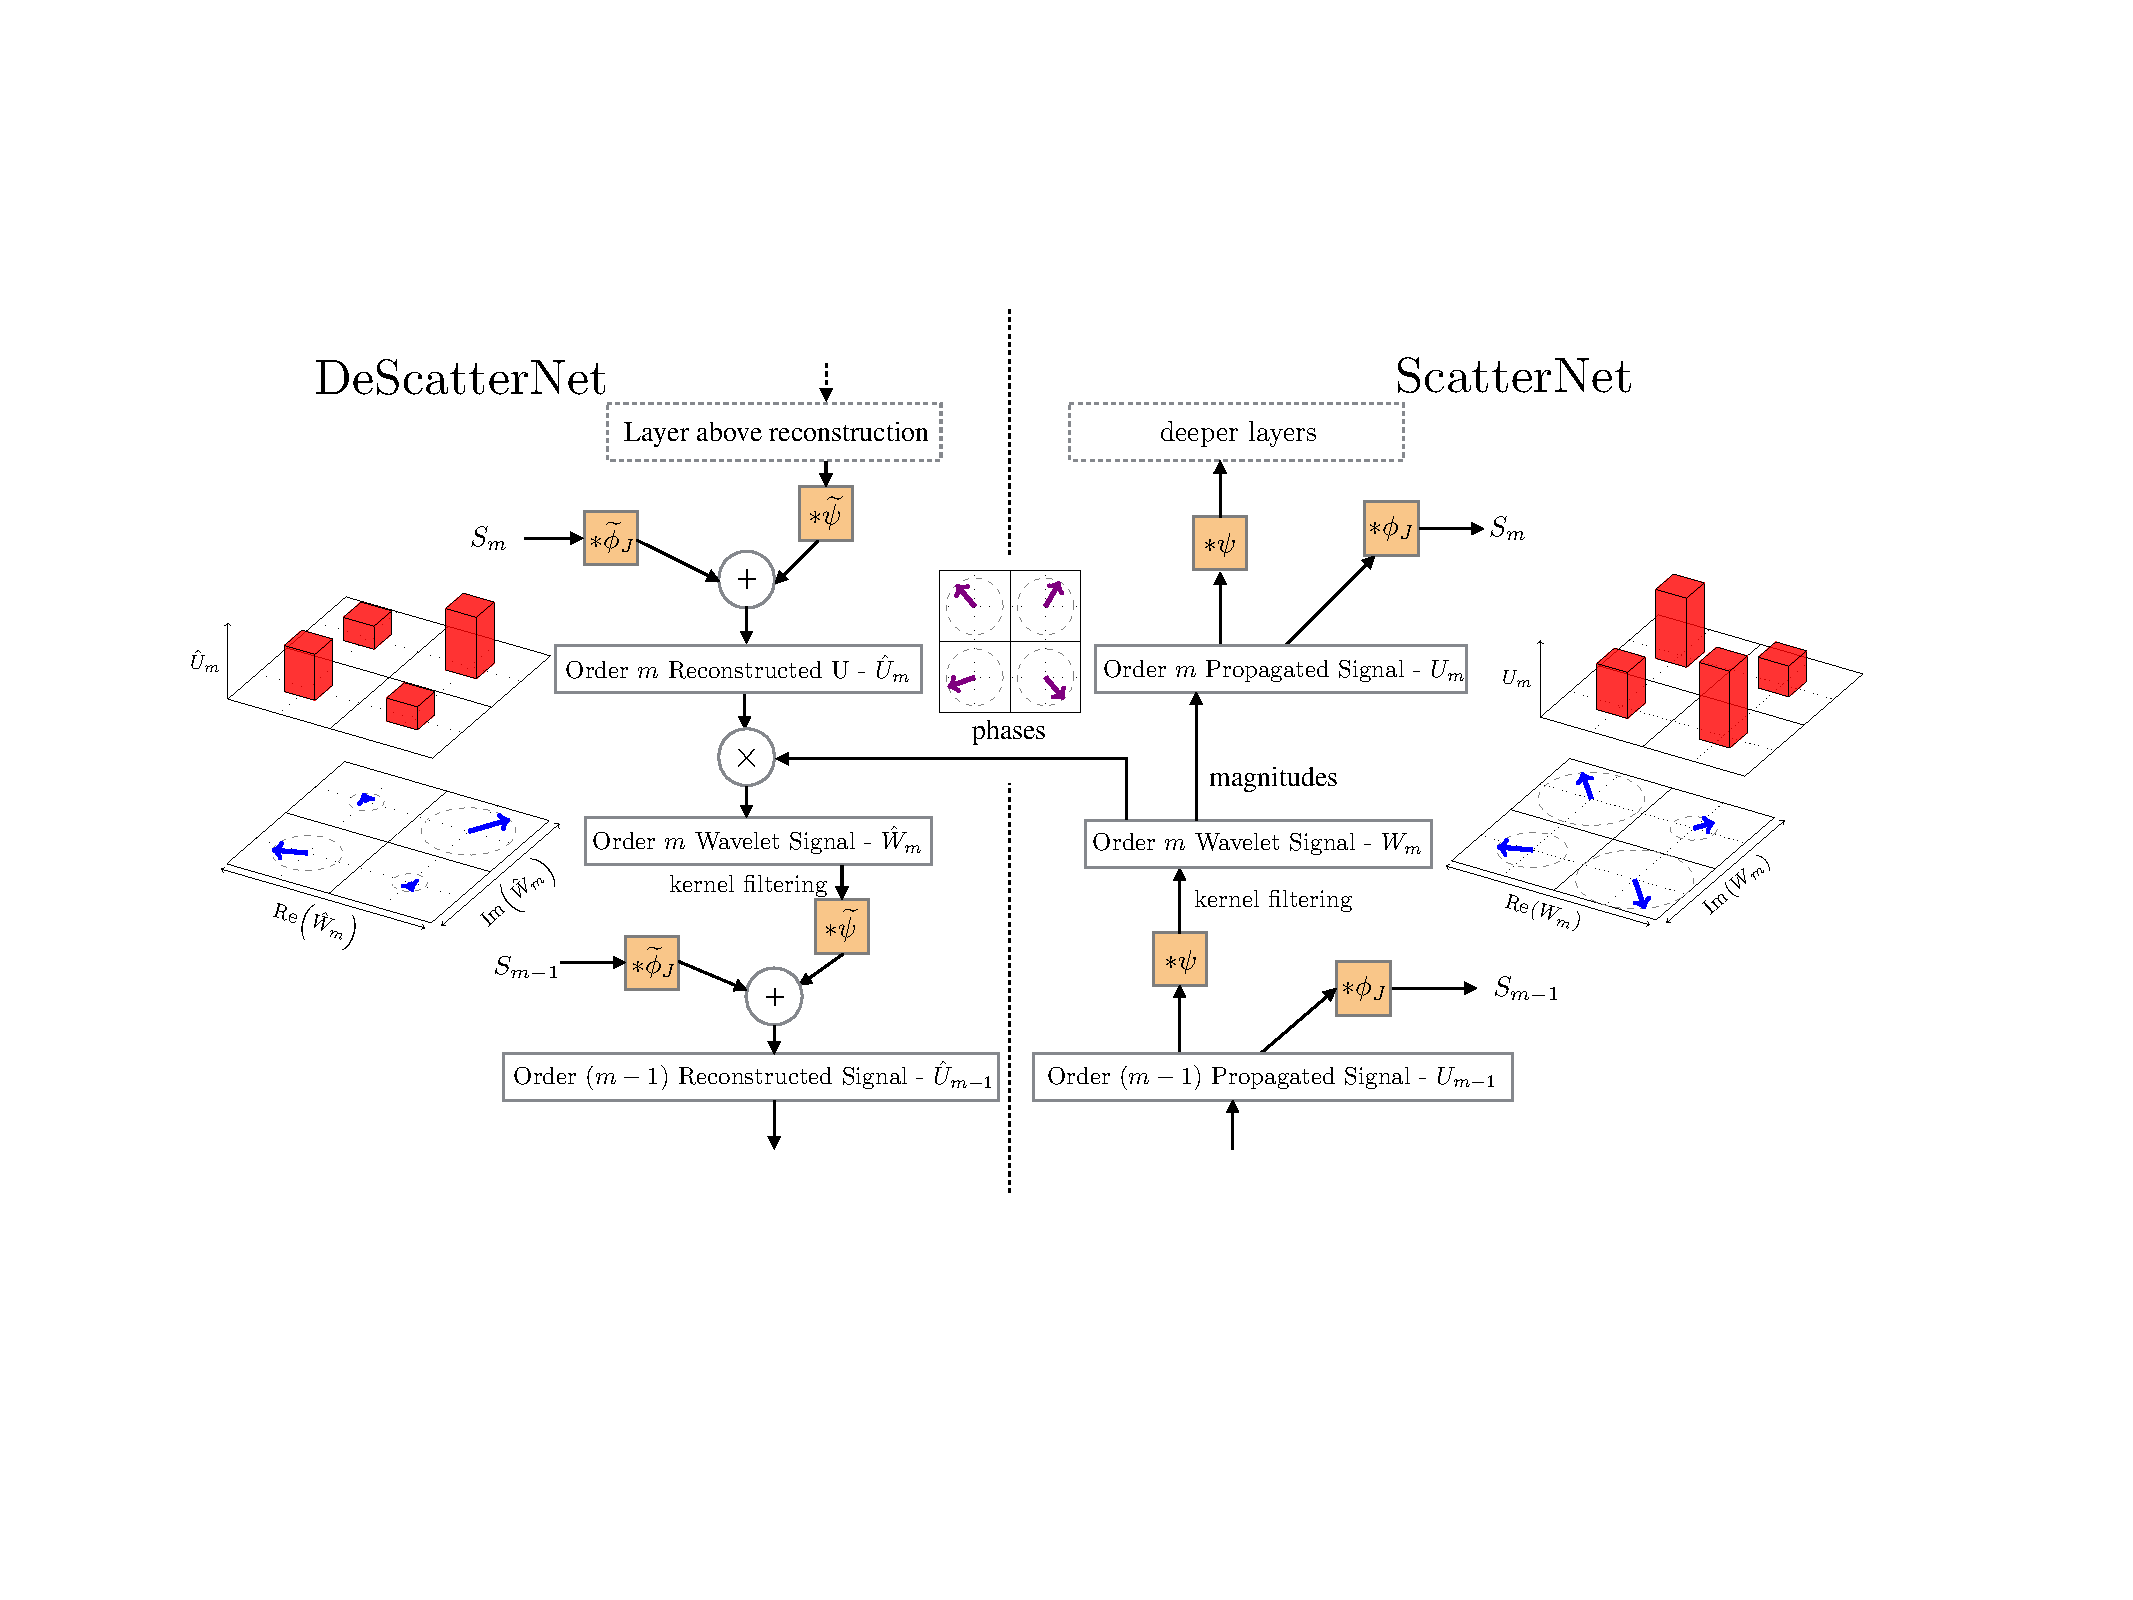
\includegraphics[width=\textwidth, trim={3cm 7cm 4cm 6cm},clip]{\imgpath/descat.pdf}
  \mycaption{The inverse scattering network}{Comprises a DeScattering layer (left)
  attached to a Scattering layer (right). We are using the same convention as
  \cite{zeiler_visualizing_2014} Figure 1 - i.e., the input signal starts in the
  bottom right-hand corner, passes forwards through the ScatterNet (up the right
  half), and then is reconstructed in the DeScatterNet (downwards on the left
  half). The DeScattering layer will reconstruct an approximate version of the
  previous order's propagated signal. The $2\x 2$ grids shown around the image
  are either Argand diagrams representing the magnitude and phase of small
  regions of \emph{complex} (De)ScatterNet coefficients or bar charts showing
  the magnitude of the \emph{real} (De)ScatterNet coefficients (after applying
  the modulus nonlinearity). For reconstruction, we need to save the discarded
  phase information and reintroduce it by multiplying it with the reconstructed
  magnitudes.}
  \label{fig:ch4:descat}
\end{figure}

We now introduce our inverse scattering network. This allows us to back-project
scattering coefficients to the image space; it is inspired by the
DeconvNet used by Zeiler and Fergus in
\cite{zeiler_visualizing_2014} to look into the deeper layers of CNNs. Like
the DeConvNet, the inverse scattering network is similar to backpropagating a
single strong activation (rather than the usual gradient terms).

We emphasize that instead of thinking about perfectly reconstructing $x$ from
$S\in \reals[C\x H'\x W']$, we want to see what signal/pattern in the input image caused
a large activation in each channel. This can then give us a good idea of what each
output channel is sensitive to, or what the ScatterNet is `extracting' from the input.
Note that we do not use any of the log normalization layers described in
\cite{oyallon_deep_2015, singh_dual-tree_2017}.

\subsection{Inverting the Low-Pass Filtering}
Going from the $U$ coefficients to the $S$ coefficients in the forward pass involves convolving by
a low pass filter $\phi_J$, possibly followed by decimation to make the output $(H\x
2^{-J})\x (W\x2^{-J})$.  $\phi_J$ is a purely real filter, and we can `invert'
this operation by interpolating $S$ to the same spatial size as $U$ and convolving with
the mirror image of $\phi_J$, $\widetilde{\phi}_J$ (this is equivalent to the
transpose convolution described in \cite{zeiler_visualizing_2014}).
\begin{equation}
  \label{eq:ch4:s_hat}
  \hat{S}_{m}x = (S_{m}x) \conv \widetilde{\phi}_J
\end{equation}
% This will not recover $U$ as it was on the forward pass, but will recover all
% the information in $U$ that caused a strong response in $S$.
We note that
interpolation usually involves lowpass smoothing of the signal, so this can all
be one operation.
% However this has
% the undesirable effect of creating multiple impulses in the next layer down's
% activations. When the next layer down is the image space this is not a problem,
% but when it is

\subsection{Inverting the Magnitude Operation}
In the same vein as \cite{zeiler_visualizing_2014}, we face a difficult
task in inverting the nonlinearity in our system.
% It has been proven that for
% particular wavelets, we can recover the phase from their modulus
% \cite{waldspurger_phase_2012}, but this is not a trivial operation. Instead, we
We lend inspiration from the switches introduced in the DeconvNet; the
switches in a DeconvNet save the location of maximal activations so that
on the backwards pass activation layers could be unpooled trivially. We do an
equivalent operation by saving the \emph{phase} of the complex activations.
On the backwards pass we reinsert the phase\footnote{We note that this is equivalent 
to finding the gradient through the magnitude operation, just as the `switches' 
from \cite{zeiler_visualizing_2014} are equivalent to taking the gradient of 
the max pooling layer.} to give our recovered $W$:
\begin{equation}
  \label{eq:ch4:w_hat}
  \hat{W}_{m}x = \left(\hat{U}_{m} x\right) e^{j\theta_{m}}
\end{equation}

\subsection{Inverting the Wavelet Decomposition}
Using the $\DTCWT$ makes inverting the wavelet transform simple, as we
can simply feed the coefficients through the synthesis filter banks to regenerate
the signal. For complex $\psi$, this is convolving with the conjugate transpose
$\widetilde{\psi}$:
\begin{eqnarray}
  \label{eq:ch4:x_hat}
  \hat{U}_{m-1}x &=& \hat{S}_{m-1}x + \hat{W}_{m}x \\
                 &=& (S_{m-1}x) \conv \widetilde{\phi}_J + \sum_{\lambda_m} \left(\hat{U}_m x\right) e^{j\theta_m}
  \conv \widetilde{\psi}_{\lambda_m}
\end{eqnarray}

\subsection{The $\DTCWT$ ScatterNet}
The combination of the above three stages can be repeated for higher orders. The
resulting DeScatterNet is shown in \autoref{fig:ch4:descat}.

For the $\DTCWT$ ScatterNet (from \autoref{alg:ch3:dtcwt_scat}), this is the same
as finding the \emph{gradient} from the corresponding channels in $Z$.

\section{Visualization with Inverse Scattering}
{
\renewcommand{\_}{\textscale{.6}{\textunderscore}}
\label{sec:ch4:visualization}

We scatter all of the images from ImageNet's validation set and record the top 9
images which most highly activate each of the $C$ channels in the ScatterNet.
This is the \emph{identification} phase (in which no inverse scattering is
performed).

Then, in the \emph{reconstruction} phase, we load in the $9\x C$ images and
scatter them one by one. We take the resulting 52 channel output vector and mask
all but the largest value in the channel we are currently
examining and mask all values in the other channels.
This 1-sparse tensor is then presented to the inverse scattering network from
\autoref{fig:ch4:descat} and projected back to the image space.

Some results of this are shown in \autoref{fig:ch4:reconstructions} for the
first and second-order coefficients. For a given output channel, we show the top
9 activations projected independently to pixel space. We also show the patch
of pixels in the input image which cause this large output. As there are 12
$S_1$ coefficients, we randomly choose 3 orientations from $S_1^1$ and 3 from $S_1^2$.
Similarly, there are 36 $S_2$ coefficients, so we randomly choose 16 of these.

The order 0 and order 1 scattering (labelled with `Order 1' in
\autoref{fig:ch4:reconstructions}) coefficients look quite similar to the first
layer filters from the well-known AlexNet CNN \cite{krizhevsky_imagenet_2012}.
This is not too surprising, as the first-order scattering coefficients are
simply a wavelet transform followed by average pooling. They are responding to
images with strong edges aligned with the wavelet orientation.

The second-order coefficients (labelled with `Order
2' in \autoref{fig:ch4:reconstructions}) appear very similar to the order
1 coefficients at first glance.
They too are sensitive to edge-like features, and some of them (e.g.\ third row,
third column and fourth row, second column) are mostly just that. These are
features that have the same oriented wavelet applied at both the first and
second-order ($\theta_1 = \theta_2$). Others, such as the nine in the top left
square (first row, first column), and top right square (first row, fourth
column) are more sensitive to checker-board like patterns. These are
activations where the orientation of the wavelet for the first and second-order
scattering were far from each other ($15\degs$ and $105\degs$ for the first row,
first column and $105\degs$ and $45\degs$ for the first row, fourth column).

For comparison, we include reconstructions from the second layer of the
well-known VGG CNN\@ (labelled with `VGG conv2\_2', in
\autoref{fig:ch4:reconstructions}). These were made with a DeconvNet, following the
same method as \cite{zeiler_visualizing_2014}. Note that while some of
the features are edge-like, we also see higher-order shapes like corners,
crosses and curves.

These reconstructions show that higher-order features from ScatterNets vary
significantly from those learned in CNNs. In many
respects, the features extracted from a CNN like VGGNet look preferable for use
as part of a classification system.
\begin{figure}[tp]
  \centering
  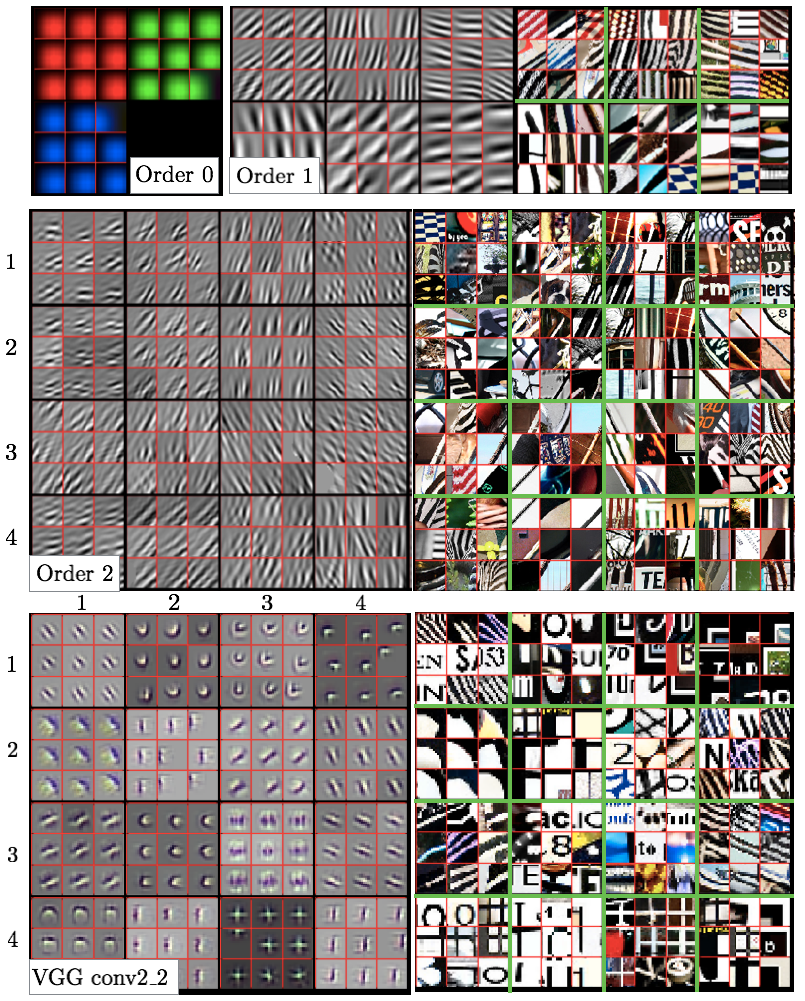
\includegraphics[width=0.9\textwidth]{\imgpath/deconv_images.png}
  \mycaption{Comparison of scattering to convolutional features}{Visualization
  of a random subset of features from $S_0$ (all 3), $S_1$ (6 from the 12) and
  $S_2$ (16 from the 36) scattering outputs. We record the top 9 activations for
  the chosen features and project them back to the pixel space. We show them
  alongside the input image patches which caused the large activations. We also
  include reconstructions from layer conv2\_2 of VGG Net
  \cite{simonyan_very_2014}(a popular CNN, often used for feature extraction)
  for reference --- here we display 16 of the 128 channels. The VGG
  reconstructions were made with a CNN DeconvNet based on
  \cite{zeiler_visualizing_2014}. Image best viewed digitally.}
  \label{fig:ch4:reconstructions}
\end{figure}

}

% \section{Implementation Details}\label{sec:implementation}
Again, we use the $\DTCWT$ \cite{selesnick_dual-tree_2005} for our wavelet filters
$\psi_{j, \theta}$ due to their fast implementation with separable convolutions
which we will discuss more in \autoref{sec:computation}.  There are two side
effects of this choice. The first is that the number of orientations of wavelets
is restricted to $K=6$. The second is that we naturally downsample the output
activations by a factor of $2$ for each direction for each scale $j$, giving a 
$4^j$ downsampling factor overall. This represents the
source of the invariance in our layer. If we do not wish to downsample the
output (say to make the layer fit in a larger network), we can bilinearly
interpolate the output of our layer. This is computationally cheap to do on its
own, but causes the next layer's computation to be higher than necessary (there
will be almost no energy for frequencies higher than $f_s/4$).

In all our experiments we set $J=1$ for each invariant layer,
meaning we can mix the lowpass and bandpass coefficients at the same resolution.
\autoref{fig:block_diagram} shows how this is done. Note that setting $J=1$ for
a single layer does not restrict us from having $J>1$ for the entire system, as
if we have a second layer with $J=1$ after the first, including downsampling
($\downarrow$), we would have:
%
\begin{equation}
  \left(\left(\left(x \conv \phi_1\right) \downarrow 2\right) \conv \psi_{1, \theta}\right) 
    \downarrow 2 = \left(x \conv \psi_{2, \theta}\right) \downarrow 4
\end{equation}

\subsection{Parameter Memory Cost}\label{sec:memory}
A standard convolutional layer with $C_l$ input channels, $C_{l+1}$ output channels
and kernel size $L\x L$ has $L^2C_{l}C_{l+1}$ parameters. 

The number of learnable parameters in each of our proposed invariant layers with
$J=1$ and $K=6$ orientations is:
%
\begin{equation}
  \text{\#params} = (JK+1)C_{l}C_{l+1} = 7C_{l}C_{l+1}
\end{equation} 
%
The spatial support of the wavelet filters is typically $5\x 5$ pixels or more,
and we have reduced $\text{\#params}$ to less than $3\x3$ per filter, while
producing filters that are significantly larger than this.

\subsection{Activation Memory Cost}
A standard convolutional layer needs to save the activation $x^{(l)}$ to
convolve with the backpropagated gradient $\dydx{L}{y^{(l+1)}}$ on the backwards
pass (to give $\dydx{L}{w^{(l)}}$). For an input with $C_l$ channels of spatial size $H\x W$, this means
$HWC_l$ floats must be saved. 

Our layer requires us to save the activation
$z^{(l+1)}$ for updating the $\tilde{a}$ terms. This has $7C_l$ channels of
spatial size $\frac{HW}{4}$. This means that our proposed layer needs to save
$\frac{7}{4}HWC_l$ floats, a $\frac{7}{4}$ times memory increase on the standard
layer.

\begin{algorithm}[tb]
\caption{Locally Invariant Convolutional Layer forward and backward
passes}\label{alg:ch6:inv}
\begin{algorithmic}[1]
\Procedure{GAINLAYERFWD}{$x,\ g_{lp},\ g_1$}
\State $u_{lp},\ u_{1} \gets \DTCWT(x^l, \mbox{nlevels}=1) $ \Comment{$u_{1}$ has 6 orientations and is complex}
  \State \textbf{save} $u_{lp},\ u_{1}$ \Comment{For the backwards pass}
  \State $v_{lp} \gets u_{lp} \conv g_{lp}$ 
  \For{$1\leq k \leq 6$}
  \State \begin{varwidth}[t]{\linewidth}  $v_{1,k} \gets 
      \left( \real{u_{1,k}} \conv \real{g_{1,k}} - \imag{u_{1,k}} \conv \imag{g_{1,k}} \right)\ +$ \par
      \hskip\algorithmicindent \hphantom{abc}$ j\left(\real{u_{1,k}} \conv \imag{g_{1,k}} + \imag{u_{1,k}} \conv \real{g_{1,k}}\right)$;
  \end{varwidth}
  \EndFor
  \State $y \gets \DTCWT^{-1}(v_{lp}, v_{1})$
  \State \textbf{return} $y$
\EndProcedure
\end{algorithmic}\vspace{10pt}
\begin{algorithmic}[1]
  \Procedure{GAINLAYERBWD}{$\dydx{L}{Y},\ g_{lp},\ g_1$}
  \State \textbf{load} $u_{lp},\ u_1$
  \State \textbf{return} $\dydx{L}{x},\ \dydx{L}{A}$
\EndProcedure
\end{algorithmic}
\end{algorithm}



\subsection{Computational Cost}\label{sec:computation}
A standard convolutional layer with kernel size $L\x L$ needs $L^2C_{l+1}$
multiplies per input pixel (of which there are $C_{l}\x H\x W$).

As mentioned in \autoref{sec:memory}, we use the $\DTCWT$ for our complex, shift
invariant wavelet decomposition. We use the open source Pytorch implementation
of the $\DTCWT$ \cite{cotter_pytorch_2018} as it can run on GPUs and
has support for backpropagating gradients.

There is an overhead in doing the wavelet decomposition for each input channel.
A separable 2-D discrete wavelet transform (DWT) with 1-D filters of length $L$
will have $2L\left(1-2^{-2J}\right)$ multiplies per input pixel for a $J$ scale
decomposition. A $\DTCWT$ has 4 DWTs for a 2-D input, so its cost is
$8L\left(1-2^{-2J}\right)$, with $L=6$ a common size for the filters. It is
important to note that unlike the filtering operation, this does not scale with
$C_{l+1}$, the end result being that as $C_{l+1}$ grows, the cost of $C_l$
forward transforms is outweighed by that of the mixing process whose cost is
proportional to $C_l C_{l+1}$.

Because we are using a decimated wavelet decomposition, the sample rate
decreases after each wavelet layer. The benefit of this is that the mixing
process then only works on one quarter the spatial size after the first scale
and one sixteenth the spatial after the second scale. Restricting ourselves to
$J=1$ as we mentioned in \autoref{sec:implementation}, the computational cost is
then:

\begin{equation}
  % \frac{7}{4}C_{l+1} + 48 \label{eq:comp}
  \underbrace{ \frac{7}{4}C_{l+1} }_{\textrm{mixing}} +
  \underbrace{\vphantom{\frac{7}{4}} 36}_{\DTCWT} \quad
  \textrm{multiplies per input pixel}\label{eq:ch5:comp}
\end{equation}
In most CNNs, $C_{l+1}$ is several dozen if not several
hundred, which makes \eqref{eq:ch5:comp} significantly smaller than
$L^2C_{l+1}=9C_{l+1}$ multiplies for $3\x 3$ convolutions.

\subsection{Forward and Backward Algorithm}
There are two layer hyperparameters to choose in our layer:
\begin{itemize}
  \item The number of output channels $C_{l+1}$. This may be restricted by the
    architecture.
  \item The variance of the weight initialization for the mixing matrix $A$.
\end{itemize}

Assuming we have already chosen these values, 
then the forward and backward algorithms can be computed with
Algorithm~\autoref{alg:ch5:inv}.


% \section{Experiments}\label{sec:experiments}
In this section we examine the effectiveness of our invariant layer by testing
its performance on the well known datasets (listed in the order of increasing
difficulty):
\begin{itemize}
  \item MNIST: 10 classes, 6000 images per class, $28\x 28$ pixels per image.
  \item CIFAR-10: 10 classes, 5000 images per class, $32\x 32$ pixels per image.
  \item CIFAR-100: 100 classes, 500 images per class, $32\x 32$ pixels per image. 
  \item Tiny ImageNet\cite{li_tiny_nodate}: 200 classes, 500 images per class, 
    $64 \x 64$ pixels per image. 
\end{itemize}
Our experiment code is available at
\url{https://github.com/fbcotter/invariant_convolution}.

\subsection{Layer Introduction with MNIST}\label{sec:ch5:mnist}
To begin experiments on the proposed locally invariant layer, we look at how
well a simple system works on MNIST, and compare it to an equivalent system with
convolutions. To minimize the effects of learning from other layers, we build a
custom small network, as described in \autoref{tab:ch5:mnist_arch}.

The first two layers are learned convolutional/invariant layers, followed by
a fully connected layer with fixed weights that we can use to project down to
the number of output classes. Finally, we add a small learned layer that
linearly combines the 10 outputs from the random projection, to give 10 new
outputs. This is to facilitate reordering of the outputs to the correct class.
This simple network is meant to test the limits of our layer, rather than
achieve state of the art performance on MNIST.

Given that our layer is quite different to a standard convolutional layer, we
must do a full hyperparameter search over optimizer parameters such as the
learning rate, momentum, and weight decay, as well layer hyperparameters 
such as the variance of the random initialization for the mixing matrix $A$.

To simplify the weight variance search, we use Glorot Uniform Initialization
\cite{glorot_understanding_2010} and only vary the gain value $a$:
%
\begin{equation}
  A_{ij} \drawnfrom U\left[ -a\sqrt{\frac{6}{(C_l + C_{l+1})HW}},\ a\sqrt{\frac{6}{(C_l + C_{l+1})HW}}\
  \right] \label{eq:ch5:glorot}
\end{equation}
%
where $C_l,\ C_{l+1}$ are the number of input and output channels as before, and
the kernel size is $H = W = 1$ for an invariant layer and $H = W= 3$ for a
convolutional layer.

We do a grid search over these hyperparameters and use Hyperband
\cite{li_hyperband:_2016} to schedule early stopping of poorly performing runs.
Each run has a grace period of 5 epochs and can train for a maximum of 20
epochs. We do not do any learning rate decay.  We found the package Tune
\cite{liaw2018tune} was very helpful in organising parallel distributed training
runs.  
% Finally, we use fANOVA \cite{hutter_efficient_2014} analysis
% to find the importance of these hyperparameters to our layer, comparing to a
% standard layer. 
The hyperparameter options are described in
\autoref{tab:ch5:hyper_options}, note that we test $4^4=256$ different options.

Once we find the optimal hyperparameters for each network, we then run the two
architectures 10 times with different random seeds and report the mean and variance of
the accuracy. The results of these runs are listed in
\autoref{tab:ch5:mnist_initial_results}.

\begin{table}[t]
  \renewcommand{\arraystretch}{1.4}
  \centering
  \mycaption{Architectures for MNIST hyperparameter experiments}{The activation
  size rows are offset from the layer description rows to convey the input and
  output shapes. The `project' layers in both architectures are unlearned, so all
  of the learning has to be done by the first two layers and the reshuffle
  layer.}
  \label{tab:ch5:mnist_arch}
  \subfloat[Reference Arch with $3\x 3$ convolutions]{%
    \label{tab:ch5:mnist_arch_conv}
    \begin{tabular}{c c}
      \toprule
      Activation Size & Layer Name + Info \\
      \midrule
      \begin{tabular}{@{}c@{}} % This supresses the space on the left and right
        $1\x 28 \x 28$ \\ $7\x 28\x 28$ \\ $7\x 14\x 14$ \\ $49\x 14\x 14$ \\ $49\x 7\x 7$ 
        \\ $2401\x 1$ \\ $10\x 1$ \\ $10\x 1$ 
      \end{tabular} &
      \begin{tabular}{@{}c@{}}
        conv1, $w \in \reals[7\x 1\x 3 \x 3]$ \\ maxpool1, $2\x 2$ \\ 
        conv2 $w \in \reals[49\x 7 \x 3\x 3]$ \\ maxpool2, $2\x 2$ \\ unravel \\
        project, $w \in \reals[2401\x 10]$ \\ reshuffle, $w\in \reals[10\x 10]$
      \end{tabular} \\
      \bottomrule
    \end{tabular}
  }\quad
  \subfloat[Invariant Architecture]{%
    \label{tab:ch5:mnist_arch_inv}
    \begin{tabular}{c c}
      \toprule
      Activation Size & Layer Name + Info \\
      \midrule
      \begin{tabular}{@{}c@{}} % This supresses the space on the left and right
        $1\x 28 \x 28$ \\ $7\x 14\x 14$ \\ $49\x 7\x 7$ \\ $2401\x 1$ \\ $10\x 1$
        \\ $10\x 1$ 
      \end{tabular} &
      \begin{tabular}{@{}c@{}}
        inv1, $A \in \reals[7\x 7]$ \\ inv2, $A \in \reals[49\x 49]$ \\ unravel \\
        project, $w \in \reals[2401\x 10]$ \\ reshuffle, $w\in \reals[10\x 10]$
      \end{tabular}\\
      \bottomrule
    \end{tabular}
  }
\end{table}




\begin{table}[hbt]
  \centering
  \mycaption{Hyperparameter settings for the MNIST experiments}{The weight gain is
  the term $a$ from \autoref{eq:ch5:glorot}. Note that $\log_{10} 3.16 = 0.5$.}
  \label{tab:ch5:hyper_options}
  \begin{tabular}{c c}
    \toprule
    Hyperparameter & Values \\
    \midrule
    Learning Rate (lr) & $\left\{ 0.0316,\ 0.1,\ 0.316,\ 1 \right\}$ \\
    Momentum (mom) & $\left\{ 0,\ 0.25,\ 0.5,\ 0.9 \right\}$ \\
    Weight Decay (wd) & $\left\{ 10^{-5},\ 3.16\x 10^{-5},\ 10^{-4},\ 3.16\x 10^{-4} \right\} $\\
    Weight Gain (a) & $\left\{0.5,\ 1.0,\ 1.5,\ 2.0 \right\}$
    \\\bottomrule
  \end{tabular}
\end{table}

\begin{table}[hbt]
  \centering
  \mycaption{Architecture performance comparison}{Numbers reported are the mean
  and standard deviation of accuracy over 10 runs with the optimal
  hyperparameters, $\theta$. Note that for
  both architectures we found that $\F{lr}$ was the most important
  hyperparameter to choose correctly, and had the largest impact on the
  performance.
  % We also use
  % fANOVA\cite{hutter_efficient_2014} analysis to weight the importance of these 
  % hyperparameters. High values imply the accuracy is more sensitive to this
  % hyperparameter. 
  }
  \label{tab:ch5:mnist_initial_results}
  \begin{tabular}{@{}l c c c@{}}
    \toprule
     & &\multicolumn{2}{c}{accuracy} \\\cline{3-4}
    Architecture & $\theta = \{\F{lr}, \F{mom}, \F{wd}, \F{a}\}$ & mean & std  \\\midrule
    Convolutional & $\{0.1,\ 0.5,\ 10^{-5},\ 1.5 \}$ & 97.3 & 0.29 \\
    Invariant & $\{0.032,\ 0.9,\ 3.2\x 10^{-5},\ 1.0 \}$ & 96.6 & 0.26 \\
    \bottomrule
  \end{tabular}
\end{table}


\subsubsection{Proposed Expansions}\label{sec:ch5:mnist_initial}
The results from the previous section seem to indicate that our proposed
invariant layer is a slightly worse substitute for a convolutional layer.
However we believe that this is due to the centred nature of the wavelet bases
that were used to generate the $z$ and later the $y$ coefficients. A similar
effect was seen in the previous chapter in \autoref{fig:ch4:shapes} where the
space of shapes attainable by mixing wavelet coefficients in a $3\x 3$ area was
much richer than those attainable by only mixing in a $1\x 1$ area. 

To test this hypothesis, we change \autoref{eq:ch5:mixing} to be:
\begin{equation}
  y^{(l+1)}(f, \xy)  =  \sum_{q \in Q} z^{(l+1)}(q, \xy) \conv \left(\tilde{a}_f(q) \alpha_f(q, \xy) \right)
\end{equation}

Where $\alpha_f(q, \xy)$ is an introduced kernel designed to allow mixing of
wavelets from neighbouring spatial locations. We test a range of possible
$\alpha$'s each with varying complexity/overhead:

\begin{enumerate}[(a)]
  \item We randomly shift each of the $7C$ subbands horizontally
    by $\{-1, 0, 1\}$ pixels, and vertically by $\{-1, 0, 1\}$ pixels. This is
    determined at the beginning of a training session and is consistent between
    batches. This theoretically is free to do, but practically it involves
    convolving with a $3 \x 3$ kernel with a single $1$ and eight $0$'s.
  \item Instead of shifting impulses as in the previous option, we can shift a
    gaussian kernel by one pixel left/right and up/down, making a smoother filter. 
  \item Instead of imposing a lowpass/impulse structure, we can set $\alpha$ to
    be a random $3\x 3$ kernel. This is chosen once at the beginning of training and then
    is kept fixed between batches.
  \item We can set the $3\x 3$ kernel to be fully learned. This
    still makes for a novel layer, but now the parameter cost is 9 times higher
    than the $1\x 1$ conv layer, and 7 times higher than a vanilla $3\x 3$
    convolution.
  \item We can take the top three $3\x 3$ DCT coefficients of the $7C$
    subbands, allowing us to do something like the previous option 
    but with only a threefold parameter increase. The top three coefficients are
    the constant, the horizontal and the vertical filters.
\end{enumerate}

Again, we search over the hyperparameter space to find the optimal
hyperparameters and then run 10 runs at the best set of hyperparameters, and
report the results in \autoref{tab:ch5:mnist_new_results}. As we expected,
adding in random shifts significantly helps the invariant layer. Two systems of
note are the shifted impulse (a) system and the learned $3\x 3$ kernel (d)
system. The first improves the mean accuracy by $1.3\%$ without any extra
learning. The second improves the performance by $2.4\%$ but with a large
parameter cost. To explore an equivalent system, we also list in
\autoref{tab:ch5:mnist_new_results} a modification to the convolutional
architecture that uses $5\x 5$ convolutions and $C_1 = 10,\ C_2 = 100$ channels,
resulting in a system with comparable parameter cost to (d).

\begin{table}[hbt]
  \renewcommand{\arraystretch}{1.4}
  \centering
  \mycaption{Modified architecture performance comparison}{Numbers reported are the mean
  and standard deviation of accuracy over 10 runs with the optimal
  hyperparameters, $\theta$. We also list parameter cost and number
  of multiplies for each layer option, relative to the standard $3\x 3$
  convolutional layer to highlight the benefits/drawbacks of each option.}
  \label{tab:ch5:mnist_new_results}
  \begin{tabular}{@{}l c c c c c@{}}
    \toprule
    & & \multicolumn{2}{c}{cost} & \multicolumn{2}{c}{accuracy} \\\cline{3-4}\cline{5-6}
    Architecture & $\theta = \{\F{lr}, \F{mom}, \F{wd}, \F{a}\}$ & param & mults & mean & std  \\\midrule
    Convolutional & $\{0.1,\ 0.5,\ 10^{-5},\ 1.5 \}$ & 1 & 1 & 97.3 & 0.29 \\
    Invariant & $\{0.032,\ 0.9,\ 3.2\x 10^{-5},\ 1.0 \}$ & $\frac{7}{9}$ & $\frac{7}{36}$ & 96.6 & 0.26 \\\midrule
    Shifted impulses (a) & $\{0.32,\ 0.5,\ 10^{-4},\ 1.0 \}$ & $\frac{7}{9}$ & $\frac{7}{36}$ & 97.9 & 0.25 \\
    Shifted gaussians (b) & $\{1.0,\ 0.0,\ 10^{-5},\ 1.0 \}$ & $\frac{7}{9}$ & $\frac{7}{4}$ & 97.7 & 0.56\\
    Random $3\x3$ kernel (c) & $\{1.0,\ 0.9,\  10^{-5},\ 1.0 \}$ & $\frac{7}{9}$ & $\frac{7}{4}$ & 95.8 & 1.01\\
    Learned 3 DCT coeffs (d) & $\{1.0,\ 0.0,\ 10^{-5},\ 1.0 \}$ & $\frac{7}{3}$ & $\frac{7}{4}$ & 98.1 & 0.37\\\midrule
    Learned $3\x3$ kernel & $\{0.1,\ 0.5,\  10^{-4},\ 1.0 \}$ & \textbf{7} & $\frac{7}{4}$ & \textbf{99.0} & 0.12 \\\midrule
    Wide Convolutional & $\{0.32,\ 0.5,\ 10^{-5},\ 1.5 \}$ & 7 & 7 & 98.7 & 0.25  \\
    \bottomrule
  \end{tabular}
\end{table}


\subsection{Layer Comparison with CIFAR and Tiny ImageNet}\label{sec:conv_exp}
Now we look at expanding our layer to harder datasets, focusing more on the
final classification accuracy. We do this again by comparing to a reference
architecture. For this task, we choose a VGG-like network as our reference.
It has six convolutional layers for CIFAR and eight layers for Tiny ImageNet as shown in
\autoref{tab:arch}. The initial number of channels $C$ we use is 64. Despite
this simple design, this reference architecture achieves competitive performance
for the three datasets.

We perform an ablation study where we progressively swap out convolutional
layers for invariant layers keeping the input and output activation sizes the
same. As there are 6 layers (or 8 for Tiny ImageNet), there are too many
permutations to list the results for swapping out all layers for our locally
invariant layer, so we restrict our results to swapping 1 or 2 layers. 
\autoref{tab:conv_results} reports the top-1 classification accuracies for
CIFAR-10, CIFAR-100 and Tiny ImageNet. In addition to testing on the full
datasets we report results for a reduced training set size. In the table, `invX'
means that the `convX' layer from \autoref{tab:arch} is replaced with an 
invariant layer.

This network is optimized with stochastic gradient descent with momentum. The
initial learning rate is $0.5$, momentum is $0.85$, batch size $N=128$ and
weight decay is $10^{-4}$. For CIFAR-10/CIFAR-100 we scale the learning rate by
a factor of 0.2 after 60, 80 and 100 epochs, training for 120 epochs in total.
For Tiny ImageNet, the rate change is at 18, 30 and 40 epochs (training for 45 in total).

\begin{table}[t]
  \renewcommand{\arraystretch}{1.4}
  \centering
  \mycaption{CIFAR and Tiny ImageNet Base Architecture}{Reference architecture
  used for experiments on CIFAR-10, CIFAR-100 and Tiny ImageNet. This
  architecture is based off the VGG\cite{simonyan_very_2014} architecture. $C$ is a
  hyperparameter that controls the network width, we use $C=64$ for our initial
  tests. The activation size rows are offset from the layer description rows to
  convey the input and output shapes.}
  \label{tab:ch5:cifar_tiny_arch}
  \subfloat[CIFAR Architecture]{%
    \label{tab:ch5:cifar_arch}
    \begin{tabular}{l l}
      \toprule
      Activation Size & Layer Name + Info \\
      \midrule
      \begin{tabular}{@{}l@{}} % This supresses the space on the left and right
        $3\x 32\x 32$ \\ $C\x 32\x 32$ \\ $C \x 32\x 32$ \\ $C\x 16\x 16$ \\
        $2C\x 16 \x 16$ \\ $2C\x 16\x 16$ \\ $2C\x 8\x 8$ \\
        $4C\x 8\x 8$ \\ $4C\x 8\x 8$\\ $4C\x 1\x 1$ \\
        $10\x1$, $100\x1$ 
      \end{tabular} &
      \begin{tabular}{@{}l@{}}
        convA, $w \in \reals[C\x 3\x 3\x 3]$ \\       
        convB, $w \in \reals[C\x C\x 3\x 3]$ \\       
        pool1, max pooling $2\x 2$ \\
        convC, $w \in \reals[2C\x C\x 3\x 3]$ \\% , $\F{stride} = 2$\\       
        convD, $w \in \reals[2C\x 2C\x 3\x 3]$ \\       
        pool2, max pooling $2\x 2$ \\
        convE, $w \in \reals[4C\x 2C\x 3\x 3]$ \\ % , $\F{stride} = 2$\\       
        convF, $w \in \reals[4C\x 4C\x 3\x 3]$ \\       
        avg, $8\x 8$ average pooling \\
        fc1, fully connected layer
      \end{tabular}\\
      \bottomrule
    \end{tabular}
  }\quad
  \subfloat[Tiny ImageNet Architecture]{%
    \label{tab:ch5:tiny_arch}
    \begin{tabular}{l l}
      \toprule
      Activation Size & Layer Name + Info \\
      \midrule
      \begin{tabular}{@{}l@{}} % This supresses the space on the left and right
        $3\x 64\x 64$ \\ $C \x 64\x 64$ \\ $C\x 64\x 64$ \\ $C\x 32\x 32$ \\
        $2C\x 32 \x 32$ \\ $2C\x 32\x 32$ \\ $2C\x 16\x 16$ \\ 
        $4C\x 16\x 16$ \\ $4C\x 16\x 16$\\ $4C\x 8\x 8$ \\
        $8C\x 8\x 8$ \\ $8C\x 8\x 8$ \\ $8C\x 1$ \\ $200\x 1$
      \end{tabular} &
      \begin{tabular}{@{}l@{}}
        convA, $w \in \reals[C\x 3\x 3\x 3]$ \\       
        convB, $w \in \reals[C\x C\x 3\x 3]$ \\       
        pool1, max pooling $2\x 2$ \\
        convC, $w \in \reals[2C\x C\x 3\x 3]$ \\ %, $\F{stride} = 2$\\       
        convD, $w \in \reals[2C\x 2C\x 3\x 3]$ \\       
        pool2, max pooling $2\x 2$ \\
        convE, $w \in \reals[4C\x 2C\x 3\x 3]$\\ % , $\F{stride} = 2$\\       
        convF, $w \in \reals[4C\x 4C\x 3\x 3]$ \\       
        pool3, max pooling $2\x 2$ \\
        convG, $w \in \reals[8C\x 4C\x 3\x 3]$\\ % , $\F{stride} = 2$\\       
        convH, $w \in \reals[8C\x 8C\x 3\x 3]$ \\       
        avg, $8\x 8$ average pooling \\
        fc1, fully connected layer
      \end{tabular}\\
      \bottomrule
    \end{tabular}
  }
\end{table}


Interestingly, we see improvements when one or two invariant layers are used
near the start of a system, but not for the first layer. In particular, the best
position for the invariant layer seems to be just before a sample rate change.
Recalling that the magnitude operation in the ScatterNet effectively
demodulates the energy from higher spatial frequencies to a lower band, it
intuitively makes sense that good places for scattering layers are at
positions where you want to downsample.

\begin{table}
  \renewcommand{\arraystretch}{1.2}
  \centering
  \mycaption{Results for testing VGG like architecture with convolutional and
  wavelet gain layers on several datasets}{An architecture with `gainX' means the
  equivalent convolutional layer `convX' from \autoref{tab:ch5:arch} was swapped for
  our proposed layer. The top row is the reference architecture using all
  convolutional layers. The DWT architecture takes a single scale DWT of the
  activations at the given layer, and mixes the coefficients to get new wavelet
  coefficients. The lowpass mixing coefficients for the DWT architecture have spatial
  size $3\x 3$ and the bandpass coefficients have spatial size $1\x 1$. The
  $\DTCWT$ architecture takes a single scale $\DTCWT$ and mixes the lowpass and 
  complex bandpass coefficients. Both the lowpass and bandpass coefficients have
  spatial size $1\x 1$. Numbers are averages over 3 runs.} 
  % \begin{tabular}{@{}lllcllcll@{}}
  \begin{tabular}{@{}lcclcclcc@{}}
    \toprule
    & \multicolumn{2}{c}{CIFAR-10} & \phantom{abc} & \multicolumn{2}{c}{CIFAR-100} & \phantom{abc} & \multicolumn{2}{c}{Tiny ImgNet} \\ \cline{2-3}\cline{5-6}\cline{8-9}
    \phantom{abc} & DWT & $\DTCWT$ &&  DWT & $\DTCWT$ && DWT & $\DTCWT$ \\ \midrule
    reference & \multicolumn{2}{c}{92.6} && \multicolumn{2}{c}{72.0} && \multicolumn{2}{c}{59.3} \\ \midrule
    gainA        & & && 72.3 & 72.8 && & \\
    gainB        & & && 72.5 & 73.4 && & \\
    gainC        & & && 72.1 & 72.8 && & \\
    gainD        & & && 72.9 & 73.1 && & \\
    gainE        & & && 72.8 & 72.7 && & \\
    gainF        & & && 73.6 & 72.7 && & \\
    gainA, gainB & & && 70.6 & 72.3 && & \\
    gainB, gainC & & && 71.7 & 73.1 && & \\
    gainC, gainD & & && 71.0 & 72.4 && & \\
    gainD, gainE & & && 72.4 & 71.9 && & \\
    gainA, gainC & & && 71.8 & 73.6 && & \\
    gainB, gainD & & && 71.7 & 72.9 && & \\
    gainC, gainE & & && 71.7 & 72.2 && & \\ \midrule
    gainA-F      & & &&      &      && & \\ \bottomrule
    
  \end{tabular}\label{tab:ch6:ablation_results}
\end{table}



\subsection{Network Comparison}\label{sec:scat_exp}
In the previous section, we examined how the locally invariant layer performs when
directly swapped in for a convolutional layer in an architecture designed
for convolutional layers. In this section, we look at how
it performs in a Hybrid ScatterNet-like \cite{oyallon_hybrid_2017,oyallon_scaling_2017},
network.

To build the second order ScatterNet, we stack two invariant layers on top of each
other. For 3 input channels, the output of these layers has $3(1 +
6 + 6 +36) = 147$ channels at $1/16$ the spatial input size. We then use 4
convolutional layers, similar to convC to convF in \autoref{tab:arch} with
$C=96$. In addition, we use dropout after these later convolutional layers with drop probability $p=0.3$.

We compare a ScatterNet with no learning in between scattering orders
(ScatNet A) to one with our proposal for a learned mixing matrix $A$ (ScatNet B). Finally,
we also test the hypothesis seen from \autoref{sec:conv_exp} about putting conv
layers before an inv layer, and test a version with a small convolutional layer
before ScatNets A and B, taking the input from 3 to 16 channels, and call these ScatNet
architectures ScatNet C and D respectively.

See \autoref{tab:hybrid_scat} for results from these experiments. It is clear from
the improvements that the mixing layer helps the Scattering front end.
Interestingly, ScatNet C and D further improve on the A and B versions
(albeit with a larger parameter and multiply cost than the mixing operation). This reaffirms that there
may be benefit to add learning before as well as inside the ScatterNet.

For comparison, we have also listed the performance of other architectures as
reported by their authors in order of increasing complexity. Our proposed ScatNet D achieves
comparable performance with the the All Conv, VGG16 and FitNet architectures.
The Deep\cite{he_identity_2016} and Wide\cite{zagoruyko_wide_2016}
ResNets perform best, but with very many more
multiplies, parameters and layers.
%and
%being quick to train --- dropping the spatial size to $8\x 8$ on CIFAR after
%only two layers is unique to the ScatterNet design. 

ScatNets A to D with 6 layers like convC to convG from \autoref{tab:arch} after
the scattering, achieve $58.1, 59.6, 60.8$ and $62.1\%$ top-1 accuracy on Tiny ImageNet. As
these have more parameters and multiplies from the extra layers we exclude them
from \autoref{tab:hybrid_scat}.

\begin{table}
  \renewcommand{\arraystretch}{1.2}
  \centering
  \mycaption{Hybrid ScatterNet top-1 classification accuracies on CIFAR}{ 
  $N_l$ is the number of learned convolutional layers, \#param is the number of
  parameters, and \#mults is the number of multiplies per $3\x 32\x 32$ image. An asterisk indicates
  that the value was estimated from the architecture description.}\label{tab:ch5:hybrid_scat}
  % \hspace{-10pt}
  \begin{tabular}{@{}lccccccc@{}}
  % \begin{tabular}{@{}llllllll@{}}
    \toprule
    & \multicolumn{3}{c}{Arch. Properties} && \multicolumn{3}{c}{Top 1 Accuracies (\%)} \\\cline{2-4}\cline{6-7}
    Arch. Name \phantom{abcde} & $N_l$ &\#Mparam &\#Mmults&\phantom{ab}&CIFAR-10&CIFAR-100\\ \midrule
    Reference 1 & 6 & 2.65 & 165 && 91.2 & 70.0 \\ 
    ScatNet A & 4 & 2.60 & 165 && 89.5 & 68.2 \\ 
    ScatNet B & 6 & 2.64 & 167 && 91.5 & 70.5  \\\midrule %
    Reference 2 & 7 & 2.69 & 165 && 92.2 & 72.2  \\ 
    ScatNet C & 7 & 2.64 & 251 && 92.6 & 72.7  \\ 
    ScatNet D & 7 & 3.7 & 251 && 93.3 & 73.6 \\ \midrule 
    All Conv\cite{springenberg_striving_2014-3} & 8 & 1.4 & 281\textsuperscript{*} && 92.8 & 66.3 \\ %    & - \\
    VGG16\cite{liu_very_2015} & 16 & 138\textsuperscript{*} & 313\textsuperscript{*}  && 91.6 & -  \\ 
    FitNet\cite{romero_fitnets:_2014} & 19 & 2.5 & 382 && 91.6 & 65.0 \\ %  & - \\
    % ResNet-110\cite{he_deep_2016} & 109 & 1.7 & 255\textsuperscript{*}& 93.6 & 74.8 \\ %              &  -\\
    ResNet-1001\cite{he_identity_2016} & 1000 & 10.2 & 4453\textsuperscript{*}&& 95.1 & 77.3 \\ %              &  -\\
    WRN-28-10\cite{zagoruyko_wide_2016} & 28 & 36.5 & 5900\textsuperscript{*} && 96.1 & 81.2 \\ %    & - \\
    \bottomrule
  \end{tabular}
  \\\vspace{20pt}
  \mycaption{Hybrid ScatterNet top-1 classification accuracies on Tiny ImageNet}{ 
  $N_l$ is the number of learned convolutional layers, \#param is the number of
  parameters, and \#mults is the number of multiplies per $32\x 32\x 3$ image. An asterisk indicates
  that the value was estimated from the architecture description.}\label{tab:ch5:hybrid_scat_ti}
  \begin{tabular}{@{}llc@{}}
    \toprule
    Arch. Name & \phantom{abc} & Top-1 Acc (\%)\\\midrule
    Reference1 && \\
    ScatNet A && \\
    ScatNet B && \\\midrule
    Reference 2 && \\
    ScatNet C && \\
    ScatNet D && \\ \bottomrule
  \end{tabular}
\end{table}



% \chapter{Conclusion}\label{ch:conclusion}
\def \path {intro/}
\def \imgpath {intro/images}

In this thesis, we have examined the effectiveness of using complex wavelets as
basis functions for deep learning models. We summarize the key results we have
found before describing what we were not able to explore due to time constraints.

% We first looked at ScatterNets, a type
% of feature extractor that builds invariances using the complex magnitude
% operation, demodulating image energy towards zero. Having examined the
% properties of these ScThen we looked at a method
% that does not rely on demodulation, and simply learns complex gains for wavelet
% subbands. The input channels could then be mixed in a learned way much like a
% regular CNN convolutional layer. The first part of our research looked
% at ScatterNets as they were a promising starting point for achieving this task.

\section{Summary of Key Results}
\textbf{\Autoref{Chapter}{ch:dtcwt_scat}} shows how using the separable spatial implementation of 
the $\DTCWT$ as the chosen wavelets for the original ScatterNet design greatly
speeds up computation (see \autoref{tab:ch3:scat_speeds}). We were also able to
derive the backpropagation equations for wavelet and scattering layers, aiding
the use of ScatterNets as part of deep networks. As part of this, we tested out
the performance of the $\DTCWT$ based ScatterNet as a front end to a simple CNN for 
some small classification tasks, and compared its performance to the Morlet based system. We
found that as well as being faster, the performance was often better when using
the $\DTCWT$ wavelets \autoref{tab:ch3:comparison}. When doing these tests, we
found that of the wavelet choices available for the $\DTCWT$, those with the
fewest taps (and largest stopband gain and transition bandwidth) performed the best. This is
somewhat surprising and while we were not able to investigate why due to time
constraints, it may provide some interesting insights as to what the CNN backend 
is doing. It also may have been a side effect of the small image sizes used in the
classification task.

\textbf{\Autoref{Chapter}{ch:visualizing}} builds a visualization tool we call the
DeScatterNet. We use this to interrogate the input patches that most highly
excite the ScatterNet outputs on a subset of images from ImageNet (see
\autoref{fig:ch4:reconstructions}). We saw that
the second order scattering coefficients are most highly excited by ripple and
checkerboard like patterns. These were very different to the patters
that most highly excite filters of a CNN. We believe this may explain why
ScatterNets perform well on texture discrimination \cite{bruna_invariant_2013}
but less well on natural image classification \cite{oyallon_deep_2015}. We then
performed some occlusion tests on a hybrid network with a ScatterNet front end
and CNN backend and saw that the CNN was able to handle when the second
order scattering coefficients were zeroed out (there was only a small drop in
classification accuracy), but it suffered greatly when the zeroth or first order
coefficients were zeroed out. We also found the surprising result that on the
datasets we tested, diagonal edges were less important than their vertical or 
horizontal counterparts (\autoref{fig:ch4:occlusion1}). If the input images were
rotated by $\pm 30\degs$ then the diagonal channels became the most important.
This echoes the experiments of
\citeauthor{blakemore_development_1970}\cite{blakemore_development_1970} who
controlled the orinetation of edges exposed to kittens in their development
stage. Finally, this chapter showed some ways to expand on the ScatterNet
network\autoref{fig:ch4:newshapes}, inspiring the work of \autoref{ch:invariant}
and \autoref{ch:freqlearn}. This layer is \textbf{cheaper and quicker
theoretically?}

\textbf{\Autoref{Chapter}{ch:invariant}} reworks the ScatterNet into individual layers.
This redesign allows us to rethink how we want to use wavelets, and we introduce
the \emph{learnable ScatterNet} made up of \emph{locally invariant convolutional
layers}. Rather than applying the same layer twice to get a second order
ScatterNet, we introduce mixing across the output channels, taken after the
magnitude operation. The flexibility of the proposed layer means it can be used
in a ScatterNet-like system, where the number of output channels grows
exponentially with the number of layers, or in a CNN-like system, where the
number of output channels remains mostly constant across layers. We experimented
with both possibilities, showing that the extra learnability definitely helps
the ScatterNet style system (\autoref{tab:hybrid_scat}) and can help a CNN
(\autoref{tab:ch5:conv_results}). The demodulation of energy from the complex
modulus means that the proposed locally invariant layer can only be used a few
times. In particular, we saw that the layer performed best when used where a CNN
would naturally downsample (or pool) the input.

\textbf{\Autoref{Chapter}{ch:freqlearn}} looks at learning in the wavelet space without
taking complex magnitudes. We present the \emph{wavelet gain layer} which takes
inputs to the wavelet domain, learns complex gains to attenuate/accentuate
different subbands, mixes the subbands across the different channels and offers
the ability of returning to the pixel domain with the inverse wavelet transform.
We propose different possible nonlinearities to use in the wavelet domain and
found that while this was possible, it did not offer an advantage over learning
directly in the pixel domain (\autoref{fig:ch6:gl_results}). 

\section{Future Work}
This thesis has started to look at ways of using wavelets as basis functions for
deep learning models. Our research has found some possible ways they could be used
which offer some advantage in terms of number of parameters, interpretability
and (theoretical) computation time. But there are many things that we were not
able to try, and some of these may show that wavelets have a larger benefit than
we found.

\subsection{Faster Transforms and expanding current approaches}
Firstly, despite our best efforts in making a fast wavelet transform, the speed
of a $\DTCWT$ in \emph{Pytorch Wavelets} is slower than it could be. A $10\x 10$
convolutional filter with 100 multiplies per input pixel is roughly twice as
quick to compute as a $\DTCWT$ with 36 multiplies per pixel. We limited our
design to use high level cuDNN calls and this was the best we could do with
these primitives. We believe that any further speed up would require custom CUDA
kernels. The speed was not a problem for datasets such as CIFAR and Tiny
ImageNet, but it did prevent us from testing the wavelet gain layer and
invariant layer on ImageNet (see \autoref{app:arch} for some run times).
We believe that these layers may perform better with larger images.

Another aspect of testing larger images is the benefit of using multiple
scales in any system. Our wavelet gain layer only used the first or second scale
in our experiments, but the real benefit of decimated wavelet transforms is the
speedup they offer by allowing for multiscale approaches. Little research has
been done in splitting the input or mid-level activations into multiple scales
and learning different filters for the different scales, but some examples
include \cite{haber_learning_2017, fujieda_wavelet_2018}.

\subsection{Applications}
low dimensional medical applications
\cite{kang_deep_2017}

\subsection{ResNets and Lifting}
\begin{figure}
  \centering
  \subfloat[Residual]{
  \centering
  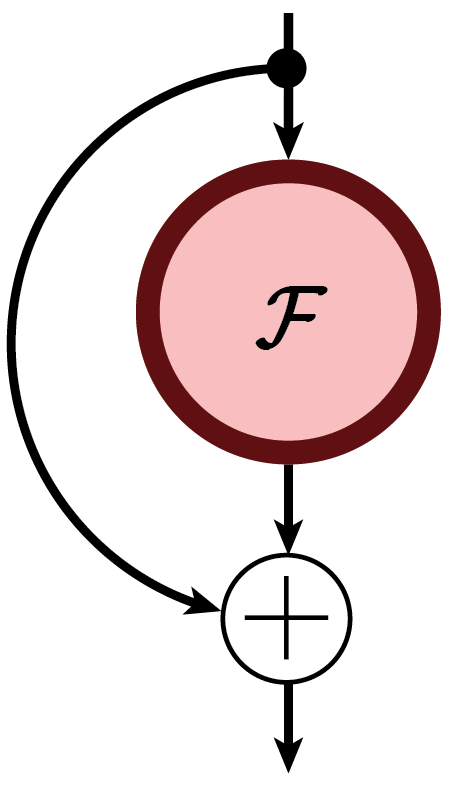
\includegraphics[width=0.13\textwidth]{\imgpath/resnet.png}
  }\qquad
  \subfloat[Lifting]{
  \centering
  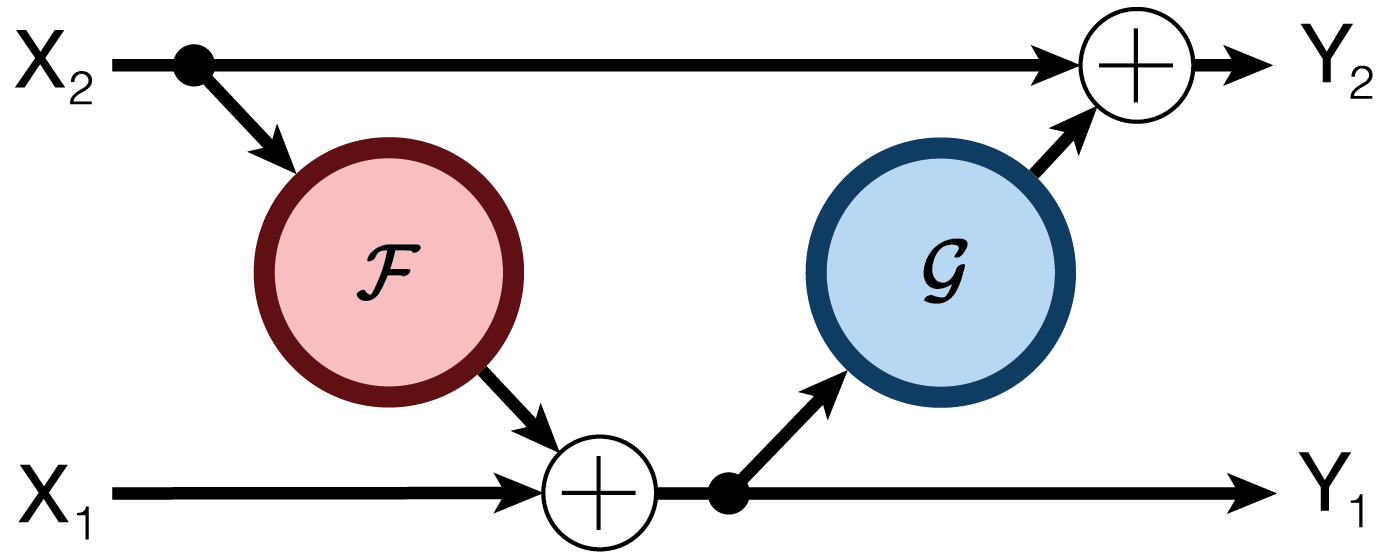
\includegraphics[width=0.48\textwidth]{\imgpath/lifting.png}
  }
  \mycaption{Residual vs Lifting Layers}{In a residual layer, an input is
  transformed by a learned function $\mathcal{F}$ and added to itself. Typically
  $\norm{\mathcal{F}x} \ll \norm{x}$ meaning the vector $y$ is a small
  perturbation of the vector $x$. In a lifting layer, each path is a learned
  function of the other added to itself. In the original second generation
  wavelets, $\mathcal{F}$ and $\mathcal{G}$ are FIR filters, but there is no
  requirement on them to be.}
  \label{fig:ch7:lifting_resnet}
\end{figure}
We briefly mentioned ResNets in \autoref{sec:ch2:resnets} but did not study them
in depth in this thesis. Interestingly, there are many similarities between
ResNets and second generation wavelets, or the \emph{lifting} framework
\cite{sweldens_lifting_1998,daubechies_factoring_1998}.
In a residual layer, the output is $y = \mathcal{F}(x) + x$, for a lifting
system, the layer is a two port network:
\begin{align}
  y_1 &= \mathcal{F}(x_1) + x_2 \\
  y_2 &= \mathcal{G}(y_1) + x_1 
\end{align}
\autoref{fig:ch7:lifting_resnet} shows the similarities between the two designs. 
\cite{gomez_reversible_2017, jacobsen_i-revnet:_2018} both make the small modifications
to the ResNet design to make a lifting style architecture.
\cite{gomez_reversible_2017} do this to save memory on the activations for
backpropagation whereas \cite{jacobsen_i-revnet:_2018} use it for its perfect
reconstruction properties. We believe that there are potentially many more
benefits to using the lifting design as an extension of our work into learning
from basis functions.

In addition to the interesting parallel between ResNets and Lifting,
\citeauthor{bartlett_gradient_2018} have found that having near identity transforms
for each stage of a deep learning system is \cite{bartlett_gradient_2018, bartlett_representing_2018}
Aside from the interesting parallel between ResNets and Lifting, ResNets have
become 
\subsection{Protecting against Attacks}
\cite{cisse_parseval_2017}

\subsection{Convolutional Sparse Coding}

\cite{liu_online_2017, liu_first_2017, papyan_convolutional_2017}

\subsection{Energy Propagation and Weight Properties}
studying the energy propagation properties and singular values of layers

Miki Elad's work on CSC.

ResNets are really good. What was the paper on that?
(Bartlett




\chapter{Visualizing and Improving Scattering Networks}\label{ch4}

% Specify the path to this folder
\def \path {visualizations/}
\def \imgpath {visualizations/images}

The drive of this thesis is in exploring if complex wavelets (in
particular the $\DTCWT$) have any place in deep learning and if they do,
quantifying how beneficial they can be. The introduction of more powerful GPUs and
fast and popular deep learning frameworks such as PyTorch, Tensorflow and Caffe
in the past few years has helped the field of deep learning grow very rapidly.
Never before has it been so possible and so accessible to test new designs and
ideas for a machine learning algorithm than today. Despite this rapid growth,
there has been little interest in building wavelet analysis software in modern
frameworks.

This poses a challenge and an opportunity. To pave the way for more detailed
investigation (both in the rest of this thesis and by other researchers
who want to explore wavelets applied to deep learning), we must have the right
foundation and tools to facilitate research.

A good example of this is the current implementation of the ScatterNet. While
ScatterNets have been the most promising start in using wavelets in a deep
learning system, they have tended to be orders of magnitude slower, and significantly more
difficult to run than a standard convolutional network.

Additionally, any researchers wanting to explore the DWT in a deep learning
system have had to rewrite the filter bank implementation themselves, ensuring they
correctly handle boundary conditions and ensure correct filter tap alignment to
achieve perfect reconstruction.

\section{Chapter Layout}
This chapter describes how we have built a fast ScatterNet implementation in
PyTorch with the $\DTCWT$ as its wavelet transform. First, we describe how to do an
efficient DWT in PyTorch in \autoref{sec:ch3:dwt} before showing how to expand this
to an efficient $\DTCWT$ in \autoref{sec:ch3:dtcwt}.
We then use the $\DTCWT$ to define our own ScatterNet in \autoref{sec:ch3:scat} (in
particular, see \autoref{alg:ch3:dtcwt_scat}). 
All of the code is available as an open-source library at \emph{PyTorch Wavelets} \cite{cotter_pytorch_2018}.

In parallel with our efforts, the original authors of the ScatterNet have
improved their implementation, making a new package called KyMatIO\cite{andreux_kymatio:_2018}. 
We compare the speed and classification performance of our package to KyMatIO in \autoref{sec:ch3:comparison}
as this provides some interesting insights into the choice of complex wavelet
for a ScatterNet. This is similar to the work of
\cite{singh_multi-resolution_2016}, where
\citeauthor{singh_multi-resolution_2016} show that a $\DTCWT$-ScatterNet
outperforms a Morlet-ScatterNet when used as a front end to an
SVM for some simpler classification tasks.
We find that our proposed $\DTCWT$-ScatterNet is 7 to 15 times faster 
than KyMatIO (depending on the padding style and wavelet length), as well as
giving a small improvement in performance when used as a front end to a CNN.

\chapter{Introduction}\label{ch:intro}

\def \path {other}
\def \imgpath {\path/images}

It has long been the goal of computer vision researchers to be able to develop
systems that can reliably recognize objects in a scene. Achieving this unlocks a huge
range of applications that can benefit society as a whole: fully
autonomous vehicles, automatic labelling of uploaded videos/images for
searching, interpretation and screening of security video feeds, and many more,
all far-reaching and extremely valuable. Many of these tasks are very tedious for humans
and would be done much better by machines if the missed-detection rate can be
kept low enough. The challenge does not lie in finding the
right application, but in the difficulty of training a computer to see.

Some of the difficulties associated with vision are the presence of nuisance
variables such as changes in lighting condition, changes in viewpoint, and
background clutter. These variables do not affect the scene but can drastically change the pixel
representation of it.
Humans, even at early stages of their lives, have little difficulty filtering
out these nuisance variables and are excellent at extracting the necessary information from a scene.
To design a robust system, it makes sense to take account of how our brains see
and understand scenes.

Unfortunately, biological vision is also a complex system. It has
more to it than simply collecting photons in the eye.
An excerpt from a recent Neurology paper \cite{raichle_two_2010} sums up the problem
well:

\begin{quotation}
It might surprise some to learn that visual information is significantly
degraded as it passes from the eye to the visual cortex. Thus, of the unlimited
information available from the environment, only about $10^{10}$ bits/sec are
deposited in the retina \ldots\ only $\sim 6\times 10^6$
bits/sec leave the retina and only $10^4$ make it to layer IV of V1
\cite{anderson_directed_2005,tor_norretranders_user_1998}. These data
clearly leave the impression that visual cortex receives an impoverished
representation of the world \ldots\ it should be noted that estimates of the
bandwidth of conscious awareness itself (i.e.,\ what we `see') are in the range
of 100 bits/sec or less\cite{anderson_directed_2005,
tor_norretranders_user_1998}.
\end{quotation}

Current video cameras somewhat act as a combination of the first and second
stage of this system, collecting photons in photosensitive sensors and then
converting this to a stream of images. Standard definition digital television
typically has
a bit rate between $3\x 10^6$ and $10^7$ bits/sec (slightly larger but comparable
to the $10^6$ bits/sec travelling through the optic nerve).

If we are to build effective vision systems, it makes sense to emulate this
compression of information between the optic nerve and the later stages of the visual
cortex. 
% The question now stands before us --- what information is kept on entry to the V1 cortex?
Hubel and Wiesel revolutionized our understanding of the V1 cortex in their Nobel prize-winning work
(awarded in 1981 in Physiology/Medicine) by
studying cats \cite{hubel_receptive_1959, hubel_receptive_1962}, macaques and spider
monkeys \cite{hubel_receptive_1968}. They found that neurons in the V1 cortex fired
most strongly when edges of a particular (i.e.,\ neuron-dependent) orientation
were presented to the animal, so long as the edge was inside the receptive field of
this neuron.
Continuing on this work, Blakemore and Cooper \cite{blakemore_development_1970}
analysed the perception of kittens that had restricted visual information
presented to them.
In one of their experiments, the kittens were kept in darkness
and then exposed for a few hours a day to only horizontal or vertical lines.
After five months, they were taken into natural environments and their reactions
were monitored. The two groups of cats would only play with objects when
presented in an orientation that matched the orientation of their original
environment. This suggest that these early layers of perception are
\emph{learned}.
% A figure of the the frequency response of the photoreceptor cells in our eyes
% to different wavelengths of light.
% \begin{figure}
  % \begin{center}
      % 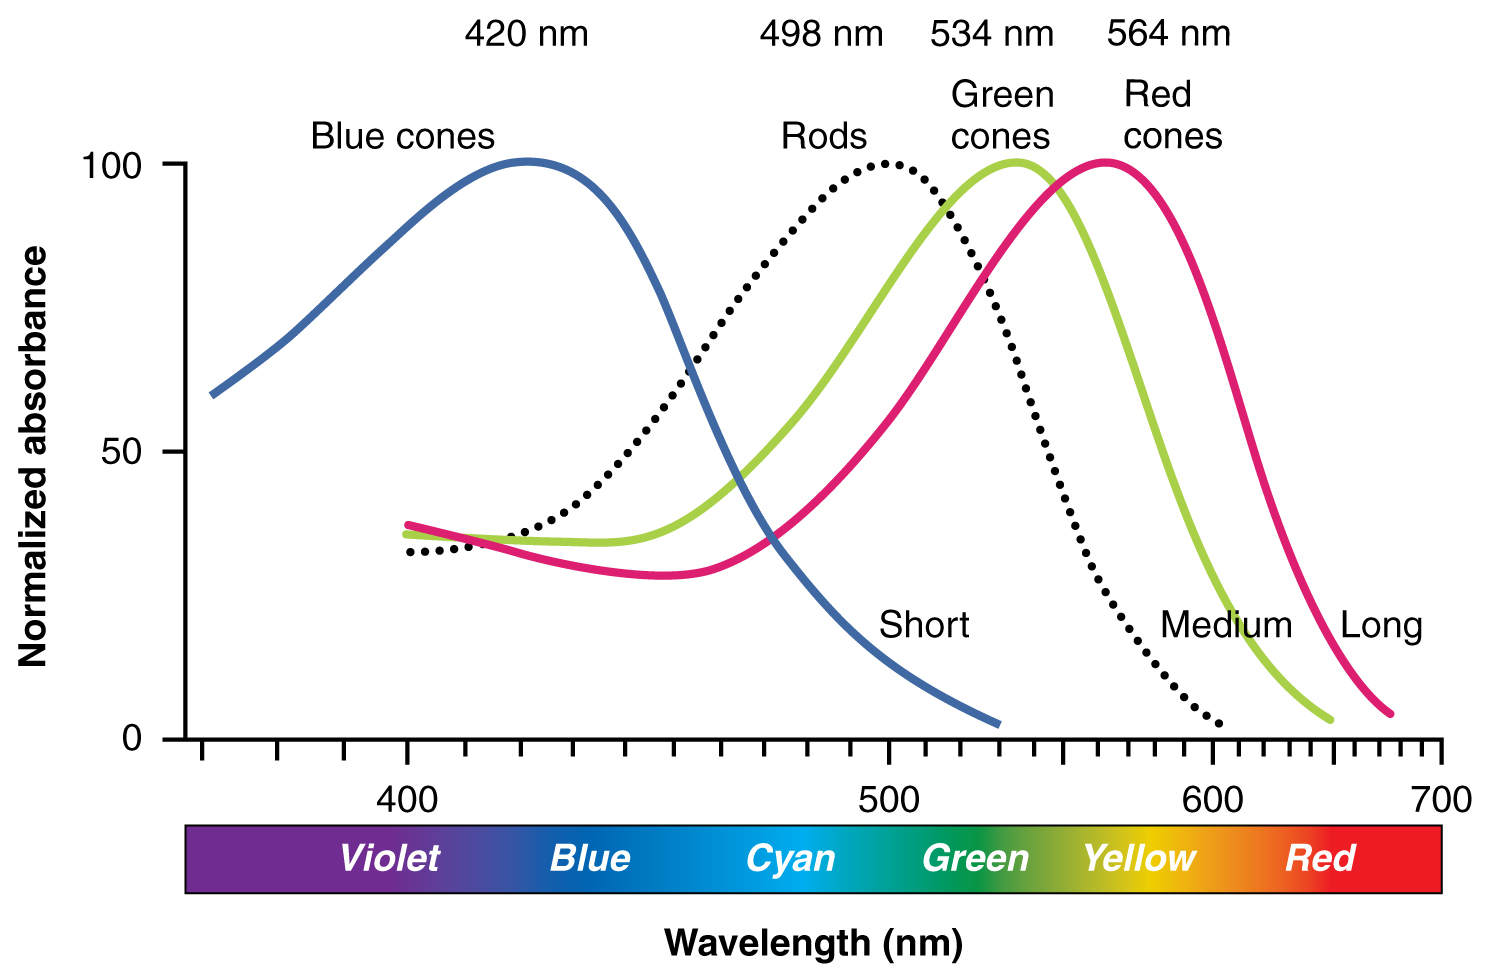
\includegraphics[width=10cm]{\imgpath/colour_sensitivity.jpg}
      % \mycaption{Frequency sensitivity of photoreceptors in they eye}
              % {Wavelength responsiveness of the different photoreceptors in the
               % eye. S, M, and L are short, medium, and long cones, compared to
               % R --- rods. Taken from~\cite{bowmaker_visual_1980}}
  % \end{center}
% \end{figure}

The current state of the art in image understanding systems are
Convolutional Neural Networks (CNNs). These are a learned model that
cascades many convolutional filters serially in layers, separated by
nonlinearities.
They are seemingly inspired by the visual cortex in the way that they are
hierarchically connected, progressively compressing the information into a
richer representation.

\autoref{fig:ch1:cnn_arch} shows an example CNN
architecture, the famous AlexNet \cite{krizhevsky_imagenet_2012}. Inputs are resized to a
manageable size, in this case, $224\x 224$ pixels. Multiple convolutional
filters of size $11\x 11$ are convolved over this input to give $96$ output
\emph{channels} (or \emph{activation maps}). In the figure, these are split onto two
graphics cards or GPUs for memory purposes. These are then passed through a
pointwise nonlinear function, or \emph{nonlinearity}.
The activations are pooled (a form of downsampling) and convolved with more
filters to give $256$ new channels at the second stage. This is repeated 3 more
times until the $13\x 13$ output with $256$ channels is unravelled and passed
through a fully connected neural network to classify the image as one of $1000$
possible classes.

CNNs have garnered lots of attention since 2012 when the previously mentioned AlexNet
nearly halved the top-5 classification error rate (from $26\%$ to $16\%$)
in the ImageNet Large Scale Visual Recognition Competition (ILSVRC)
\cite{russakovsky_imagenet_2014}\footnote{The previous state of
the art classifiers had been built by combining keypoint extractors like
SIFT\cite{lowe_distinctive_2004} and HOG\cite{dalal_histograms_2005} with
classifiers such as Support Vector Machines\cite{cortes_support-vector_1995} and
Fisher Vectors\cite{sanchez_image_2013}, for example \cite{sanchez_high-dimensional_2011}.}.
In the years since, the complexity of CNNs has grown significantly. AlexNet had
only 5 convolutional layers, whereas the 2015 ILSVRC winner ResNet \cite{he_deep_2016}
achieved 3.57\% top-5 error with 151 convolutional layers (and had some
experiments with 1000 layer networks).

\begin{figure}
  \centering
    % \includegraphics[width=\textwidth]{\imgpath/dtcwt_gain}
    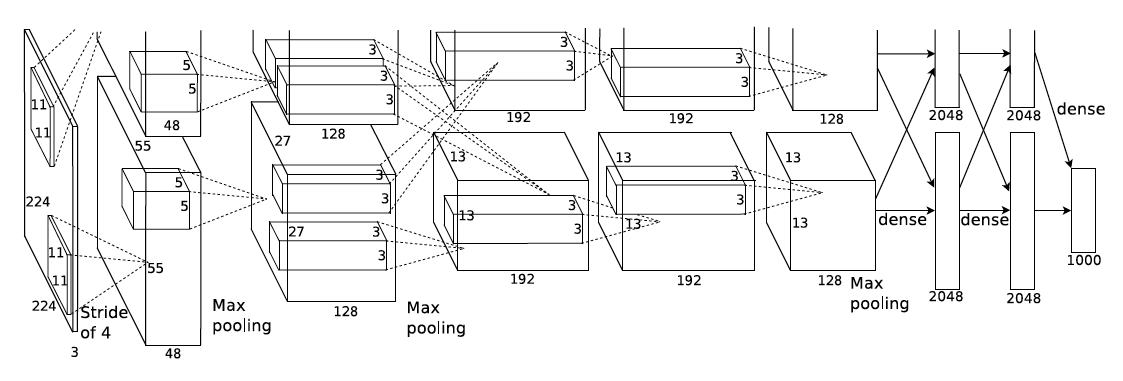
\includegraphics[width=\textwidth]{\imgpath/alexnet.png}
    \mycaption{Convolutional Architecture example}{The previous layer's activations are
    combined with a learned convolutional filter.
    Note that while the activation maps are 3-D arrays, the convolution is only
    a 2-D operation. This means the filters have the same number of channels as
    the input and produce only one output channel. Multiple channels are made by
    convolving with multiple filters. Not shown here are the nonlinearities that
    happen in between convolution operations. Image taken from \cite{krizhevsky_imagenet_2012}.}
    \label{fig:ch1:cnn_arch}
  \end{figure}

\section{Motivation}\label{sec:ch1:motivation}
\begin{figure}
  \centering
  \subfloat[conv1 filters]{
  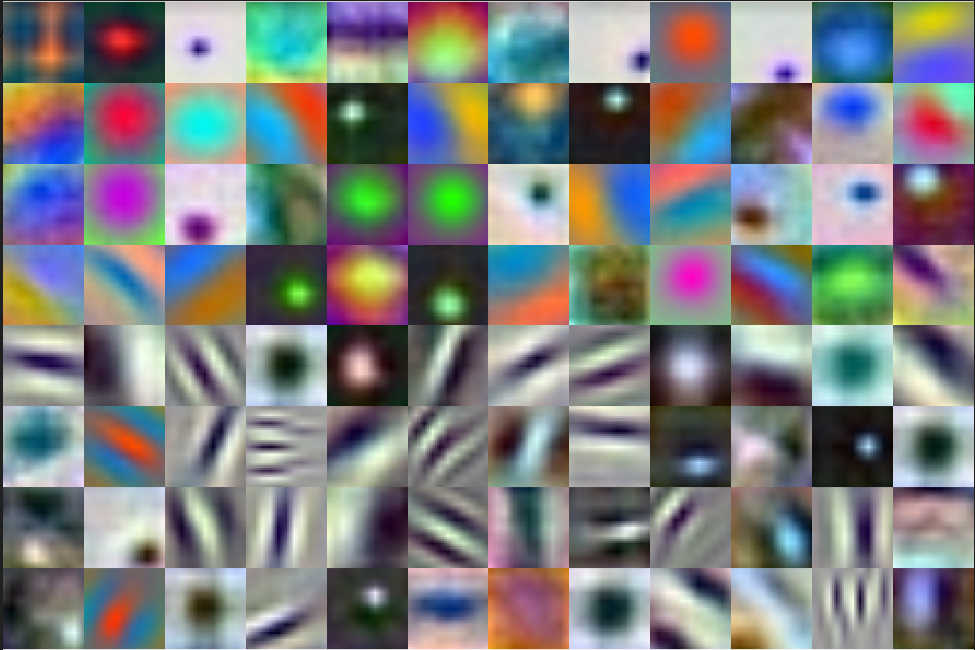
\includegraphics[width=0.6\textwidth]{\imgpath/alexfilters.png}
  \label{fig:ch1:alex_filt}
  }\\
  \subfloat[conv1 activations]{
  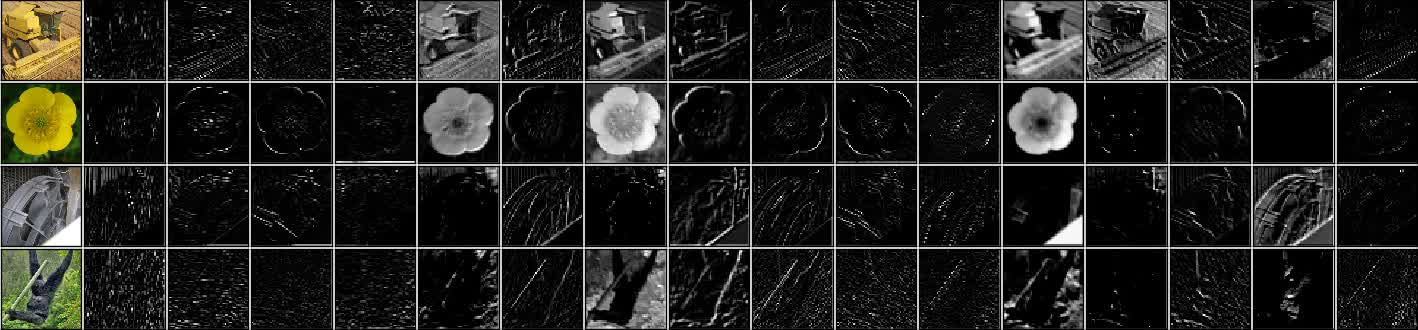
\includegraphics[width=\textwidth]{\imgpath/out1.jpg}
  \label{fig:ch1:alex_conv1}
  }\\
  \subfloat[conv2 activations]{
  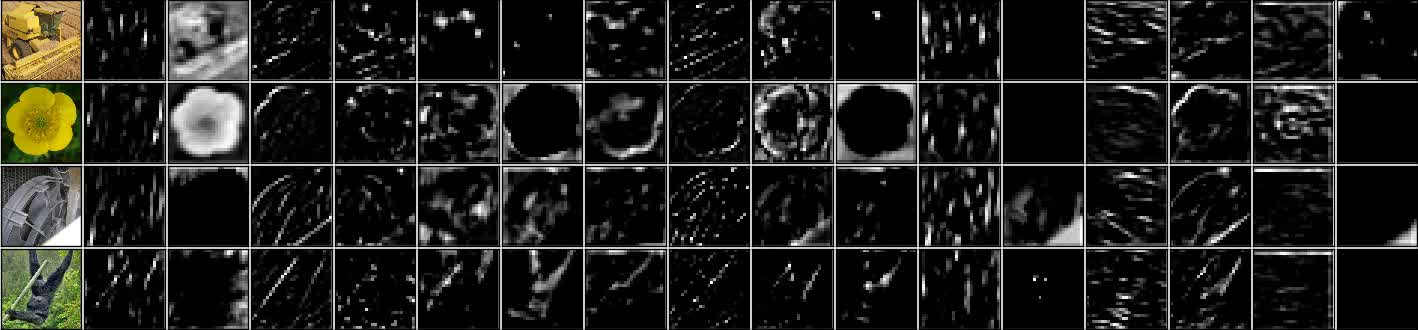
\includegraphics[width=\textwidth]{\imgpath/out2.jpg}
  \label{fig:ch1:alex_conv2}
  }\\
  \subfloat[conv3 activations]{
  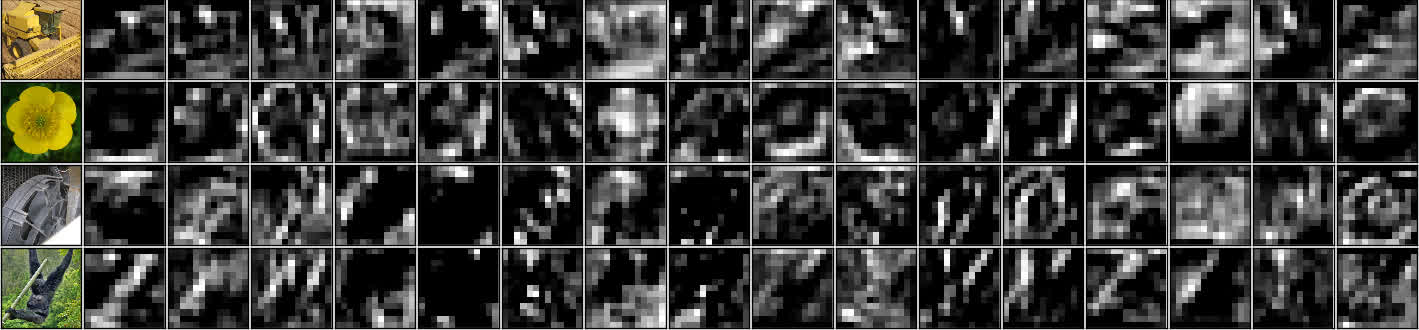
\includegraphics[width=\textwidth]{\imgpath/out3.jpg}
  \label{fig:ch1:alex_conv3}
  }
  \mycaption{Example first layer filters and the first three
  layer's outputs}{\subref{fig:ch1:alex_filt} The $11\x 11$ filters for the
  first stage of AlexNet. Of the 96 filters, 48 were learned on one GPU and
  another 48 on another GPU. Interestingly, one GPU has learned mostly
  lowpass/colour filters and the other has learned oriented bandpass
  filters. \subref{fig:ch1:alex_conv1} - \subref{fig:ch1:alex_conv3} Randomly
  chosen activations from the output of the first, second and third convolutional
  layers of AlexNet (see \autoref{fig:ch1:cnn_arch}) with negative values set to 0.
  Filters and activation images taken from supplementary material of
    \cite{krizhevsky_imagenet_2012}.}
  \label{fig:ch1:alexnet_filters}
\end{figure}

Despite their success, CNNs are often criticized for being \emph{black-box}
methods. You can view the first layer of filters
quite easily (see \autoref{fig:ch1:alex_filt}) as they exist in RGB
space, but beyond that things get trickier as the filters have a third, \emph{channel}
dimension, typically much larger than the two spatial dimensions. Additionally,
it is not clear what the input channels themselves correspond to. For illustration
purposes, we have also shown some example activations from the first three
convolutional layers for AlexNet in
\autoref{fig:ch1:alexnet_filters}\subref{fig:ch1:alex_conv1}-\subref{fig:ch1:alex_conv3}\footnote{These activations are
taken after a specific nonlinearity that sets negative values to 0, hence the
large black regions.}. For the conv1 activations in
\autoref{fig:ch1:alex_conv1}, we can accurately guess that some of the first layer
channels are responding to edges or colour information, but as we go deeper to
conv2 and conv3, it becomes less and less clear what each activation is
responding to.

This has started to become a problem, and while we are happy to trust modern
CNNs for isolated tasks, we are less likely to be comfortable with them driving
cars through crowded cities, or making executive decisions that affect people
directly. In a commonly used contrived example, it is not hard to imagine a deep
network that could be used to assess whether giving a bank loan to an applicant
is a safe investment. Trusting a black box solution is deeply unsatisfactory in
this situation. Not only from the customer's perspective, who, if declined, has
the right to know why \cite{goodman_european_2016}, but
also from the bank's --- before lending large sums of money, most banks
would like to know why the network has given the all clear. `It has worked well
before' is a poor rule to live by.

Aside from their lack of interpretability, it often takes a long time and a lot of
effort to train state-of-the-art CNNs. Typical networks that have won ILSVRC
since 2012 have had roughly 100 million parameters and take up to a week to train. This
is optimistic and assumes that you already know the necessary optimization or
architecture hyperparameters, which you often have to find out by trial and error.
In a conversation the author had with Yann LeCun, the attributed father of
CNNs, at a Computer Vision Summer School (ICVSS 2016), LeCun highlighted this problem
himself:
\begin{quote}
  There are certain recipes (for building CNNs) that work and certain recipes
  that don't, and we don't know why.
\end{quote}

Considering the recent success of CNNs, it is becoming more and more
important to understand \emph{how} and \emph{what} a network learns, so we can
interrogate what in the input has contributed to it making its classification or regression choice.
Without this information, the use of these incredibly powerful tools could be
restricted to research and proprietary applications.

\section{Approach}
The structure of convolutional layers is fairly crude in terms of signal
processing - arbitrary taps of an FIR filter are learned typically via
stochastic gradient descent from random starting states to minimize either a
mean-squared error or cross-entropy loss.

This leads us to ask a motivating question:
%
\begin{quote}
  Is it possible to learn convolutional filters as combinations of basis
  functions rather than individual filter taps?
\end{quote}

In achieving this, it is important to find ways to have an adequate
richness of filtering while reducing the number of parameters needed to specify resulting
filters. We want to contract the space of learning to a subspace or manifold that
is more useful. In much the same way, the convolutional layer in a CNN is a restricted
version of a fully connected layer in a multi-layer perceptron, yet adding this
restriction allowed us to train more powerful networks.

\begin{quote}
The intuition that we explore in this thesis is that \emph{complex wavelets} are
good basis functions for filtering in CNNs.
\end{quote}

\subsection{Why Complex Wavelets?}
Most modern approaches to CNNs are framed entirely in the spatial domain; our
choice of complex wavelets as the basis function to explore comes from the
deeper intuition that it may be helpful to rethink about CNNs in the
\emph{frequency domain}.  Historically, the frequency domain has been an
excellent space for solving many signal processing problems such as noise
removal, filter design, edge detection and data compression. We believe it may prove to
have advantages for CNNs too (beyond just an efficient space to do convolution
in).

The Fourier transform, which uses complex sinusoids as
its basis function, is perhaps the most ubiquitous tool to use for frequency
domain analysis. The problem with these complex sinusoids is that they have
\emph{infinite} support. This means that small changes in one part of an image
affect every Fourier coefficient. Additionally, they are not stable to small
deformations, as small changes can produce unbounded changes in the representation
\cite{mallat_group_2012}.

The common remedy to this problem is to use the localized, and more
stable, short-time Fourier transform (STFT). The STFT (or the Gabor transform)
is a natural extension of the Fourier transform, windowing the complex sinusoids
with a Gaussian (or similar) function. The STFT has the undesirable property that all
frequencies are sampled with the same resolution. A close relative of the STFT is the
continuous wavelet transform (CWT). The shorter duration of the wavelet basis
functions as the frequency increases means that their time resolving power
improves with centre-frequency.
Another commonly used
wavelet transform is the discrete wavelet transform (or the DWT) often favoured over
the CWT because of its speed of computation. It can use many
different finite support basis functions, all with different frequency
localization properties, but it is usually limited to using real filters. As such, it
suffers from many problems such as shift-dependence and lack of directionality in
two dimensions (2-D). These problems can be remedied by using the slower CWT with complex basis
functions, but we choose instead to use the dual-tree complex wavelet transform,
or $\DTCWT$ \cite{selesnick_dual-tree_2005} with q-shift filters \cite{kingsbury_complex_2001}.

The $\DTCWT$ allows for complex basis functions that have shift-invariance and
directionality, while being fast to implement like the DWT (in 2-D it can be thought of as the
application of 4 DWTs in parallel). It is also more easily invertible than the
CWT, forming a tight frame \cite{kovacevic_introduction_2008}, which we believe
may prove to be a very important property for visualizing what a
CNN is responding to.

We revisit the properties of the Fourier transform, STFT, CWT, DWT and $\DTCWT$
and expand on the properties behind our choice of basis functions
in the literature review \autoref{sec:ch2:fourier}.

On top of the intuition that the wavelet domain is a good space in which to frame CNNs,
there are some experimental motivating factors too. Firstly, the wavelet
transform has had much success in image and video compression, particularly for
JPEG2000 \cite{taubman_jpeg2000_2013}. Good compression performance implies an ability of
the basis functions to represent the input data sparsely (as seems to happen in
the brain). Secondly, the filters from the first layer of AlexNet
(\autoref{fig:ch1:alexnet_filters}) look like oriented wavelets. Given that
there was no prior placed on the filters to make them have this similarity to
wavelets, this result is noteworthy. And finally, the aforementioned work of
Hubel and Wiesel suggests that the early layers of the visual system act like a
Gabor transform.

These experimental observations imply that complex wavelets would do well in
replacing the first layer of a CNN, but we would aslo like to find out if they can be used
at deeper layers. Their well-understood and well-defined behaviour would help us
to answer the above \emph{how} and \emph{why} questions. Additionally, they
allow us to enforce a certain amount of smoothness and near orthogonality;
smoothness seems to be important to avoid sensitivity to adversarial or spoofing
attacks \cite{szegedy_intriguing_2014} and near orthogonality allows you to
cover a large space with fewer coefficients.

But first, we must find out \emph{if} it is possible to get the same or nearly the same
performance by using wavelets as the building blocks for CNNs, and this is the
core goal of this thesis.

\section{Method}
\subsection{ScatterNets}
To explore the uses of complex wavelets in CNNs, we begin by looking at one of the most
popular current uses of wavelets in image recognition tasks, the
Scattering Transform.

The Scattering Transform, or the \emph{ScatterNet}, was introduced in \cite{mallat_group_2012,
bruna_invariant_2013} at the same time as AlexNet. It is a non-black-box
network that can be thought of as a restricted complex-valued CNN
\cite{bruna_mathematical_2015}. Unlike a CNN, it has predefined
convolutional kernels, set to complex wavelet (and scaling) functions and uses
the complex magnitude as its nonlinearity. Due to
its well-defined structure, it can be analyzed and bounds on its stability to
shifts, noise and deformations are found in \cite{mallat_group_2012}.
%
% This is a promising start to addressing the problems of CNNs as using
% predefined, general filters helps us answer \emph{how} a CNN is
% learning, although the \emph{what} is still somewhat unclear.

For a simple task like identifying small handwritten digits,
the variabilities in the data are simple and small and the ScatterNet can easily
reduce the problem into a space which a Gaussian Support Vector Machine (or SVM
\cite{cortes_support-vector_1995}) can easily solve
\cite{bruna_invariant_2013}. For a more complex task like identifying real-world
objects, the ScatterNet can somewhat reduce the variabilities and get good
results with an SVM, but there is a significant performance gap between this and
what a CNN can achieve. For example, in \cite{oyallon_deep_2015} a second-order
ScatterNet can achieve $82.3\%$ top-1 classification accuracy on CIFAR-10, a
commonly used dataset, whereas modern CNNs such as \cite{he_deep_2016} can
achieve $93.4\%$.

\subsection{Learnable ScatterNets}
To start to address the performance gap between ScatterNet front ends and CNNs
we first investigate the properties of current ScatterNets. Inspired by the
visualization work of \citeauthor{zeiler_visualizing_2014}
\cite{zeiler_visualizing_2014} we build a DeScatterNet. The DeScatterNet
leverages the perfect reconstruction properties of the $\DTCWT$ and allows us to
investigate what in the input image the ScatterNet is responding to.

The DeScatterNet shows that the ScatterNet may be limiting itself by not
combining the filtering of different wavelet orientations (it does not mix the
channels as a CNN does). Inspired by the work of \cite{qiu_dcfnet:_2018}, we
propose the learnable ScatterNet, which includes this mixing while keeping the
desirable properties of the ScatterNet.

The learnable ScatterNet can be thought of as using the scattering outputs as
the \emph{basis functions}\footnote{Although they are not true basis functions
as they are the combination of a complex wavelet with a modulus nonlinearity,
and are thus data-dependent.} for our convolutional layers. We show that this
improves greatly on the ScatterNet design, and under certain constraints can
improve on the performance of CNNs too.

\subsection{Wavelet Domain Filtering}
We find that the complex modulus of the ScatterNet design to be useful for some
operations in a CNN, but it has a demodulating effect on the frequency energy
(all the outputs have significantly more energy in lower frequencies). This
limits repeated application of it as the demodulating effect compounds.

We develop a system that does not use the complex modulus; instead, it
learns \emph{complex} gains in the wavelet domain.
Rather than mixing subbands together, we keep them independent and only learn to
mix across the channel dimension. This is important, as it allows us to then use the inverse
$\DTCWT$ to return to the pixel domain. The shift-invariant properties of the $\DTCWT$ mean the
reconstructed outputs are (mostly) free from aliasing effects, despite much of
the processing being carried out at significantly reduced sample rates in the
wavelet domain.

We show that our layer can be used alongside regular convolutional
layers. I.e., it becomes possible to `step' into the wavelet domain to do
wavelet filtering for one layer, before `stepping' back into the pixel domain to
do pixel filtering for the next layer.

\section{Thesis Layout and Contributions to Knowledge}
This thesis has one literature review chapter and four novel-work chapters:
\begin{itemize}
\item
  \hyperref[ch:litreview]{Chapter~\ref*{ch:litreview}}
  explores some of the background necessary for starting
  to develop image understanding models. In particular, it covers the
  inspiration for CNNs and the workings of CNNs themselves, as well as covering
  the basics of wavelets and ScatterNets.
\item
  \Autoref{Chapter}{ch:dtcwt_scat} proposes a change to the core of the ScatterNet. In
  addition to performance issues with ScatterNets, they are slow and both
  memory-intensive and compute-intensive to calculate. This in itself is enough of an
  issue to make it unlikely that they would be used as part of deep networks. To
  overcome this, we change the computation to use the $\DTCWT$
  \cite{selesnick_dual-tree_2005} instead of Morlet wavelets, achieving a 20 to
  30 times speed-up while achieving a small improvement in classification performance.
\item
  \Autoref{Chapter}{ch:visualizing} describes our \emph{DeScatterNet}, a tool used to
  interrogate the structure of ScatterNets. We also perform tests to determine
  the usefulness of the different scattered outputs finding that many of them
  are not useful for image classification.
\item
  \Autoref{Chapter}{ch:invariant} describes the \emph{Learnable ScatterNet} we have developed to
  address some of the issues found from the interrogation in
  \autoref{ch:visualizing}. We find that a learnable ScatterNet layer performs
  better than a regular ScatterNet, and can improve on the performance of a CNN
  if used instead of pooling layers. We also find that scattering works well not
  just on RGB images, but can also be useful when used after one layer of
  learning.
\item
  In \autoref{ch:freqlearn}, we step away from ScatterNets and present the
  \emph{Wavelet Gain Layer}. The gain layer uses
  the wavelet space as a latent space to learn representations. We find possible
  nonlinearities and describe how to learn in both the pixel and wavelet domain.
  This work showed that there may well be benefits to learning in the wavelet
  domain for earlier layers of CNNs, but we have not yet found advantages to
  using the wavelet gain layer for deeper layers.
\end{itemize}

\subsection{Contributions and Publications}
The key contributions of this thesis are:

\begin{itemize}
  \item Software for wavelets and $\DTCWT$ based ScatterNet (described in \autoref{ch:dtcwt_scat})
    and publicly available at \cite{cotter_pytorch_2018}.
  \item ScatterNet analysis and visualizations (described in
    \autoref{ch:visualizing}). This chapter expands on the paper we presented at MLSP2017
    \cite{cotter_visualizing_2017}.
  \item Invariant Layer/Learnable ScatterNet (described in \autoref{ch:invariant})). This chapter expands
    on the paper accepted at ICIP2019 \cite{cotter_learnable_2019}. Software
    available at \cite{cotter_learnable_2019-1}.
  \item Learning convolutions in the wavelet domain (described in
    \autoref{ch:freqlearn}). We have published preliminary results on this work
    to arXiv \cite{cotter_deep_2018} but have expanded on this paper in the
    chapter. Software available at \cite{cotter_dtcwt_2018}.
\end{itemize}

\subsection{Related Research}
Readers may also be interested in the theses \cite{singh_scatternet_2018} and
\cite{oyallon_analyzing_2017}.

In \cite{singh_scatternet_2018}
\citeauthor{singh_scatternet_2018} looks at using the ScatterNet as a fixed
front end and combining it with well-known machine learning methods such as
SVMs, Autoencoders and Restricted Boltzmann Machines. By combining frameworks in
a defined way he creates unsupervised feature extractors which can then be used
with simple classifiers. Some relevant papers that makeup this thesis are \cite{singh_multi-resolution_2016,
singh_scatternet_2017, singh_generative_2018}. In
\cite{singh_multi-resolution_2016} Singh shows
that the $\DTCWT$-ScatterNet outperforms a Morlet-ScatterNet when used as a front end for
an SVM, which is similar to the work we do in \autoref{ch:dtcwt_scat} where we
show the $\DTCWT$-ScatterNet outperforms a Morlet-ScatterNet when used as a
front end for CNNs. He then expands on this work by testing other backends in
\cite{singh_scatternet_2017, singh_generative_2018}.

In \cite{oyallon_analyzing_2017}
\citeauthor{oyallon_analyzing_2017} looks at ScatterNets as front ends to
deeper learning systems, such as CNNs. Some relevant papers that makeup Oyallon's thesis are
\cite{oyallon_deep_2015, oyallon_scaling_2017, oyallon_hybrid_2017}. \cite{oyallon_scaling_2017, oyallon_hybrid_2017}
are particularly relevant as he uses a ScatterNet as a feature extractor for a
CNN. We do similar research in \autoref{ch:invariant}, but allow for
learned weights in the ScatterNet in our design.

\section{The Scattering Transform} \label{sec:ch4:scatternet}
While we have introduced the scattering transform before, we clarify the format
we use for this chapter's analysis.

We use the $\DTCWT$ based ScatterNet introduced in the previous chapter --
\autoref{alg:ch3:dtcwt_scat} as a front end, with $K=6$ orientations, $J=2$
scales and $M=2$ orders.

Consider a single-channel input signal $x(\xy)$, $\xy \in \reals[2]$.
The zeroth-order scatter coefficient is the lowpass output of a $J$
level filter bank:
%
\begin{equation}
  S_0x(\xy) \definedas x(\xy) \conv \phi_J(\xy)
\end{equation}
%
This is approximately invariant to translations of up to $2^J$ pixels\footnote{From here on,
we drop the $\xy$ notation when indexing $x$, for clarity.}. In exchange for
gaining invariance, the $S_0$ coefficients have lost information
(contained in the rest of the frequency space). The remaining energy of $x$ is
contained within the first-order \emph{wavelet} coefficients:
\begin{equation}
  W_1x(\lambda_1, \xy) \definedas x \conv \psi_{\lambda_1}
\end{equation}
for $\lambda_1 = (j_1, \theta_1)$, $j_1\in\{1, 2\}, \theta_1 = \frac{\pi +
2k\pi}{12}$ with $k \in \{0, 1, \ldots 5\}$.

Taking the magnitude of $W_1$ gives us the first-order \emph{propagated}
signals:
\begin{equation}
  U_1x(\lambda_1, \xy) \definedas |x \conv \psi_{\lambda_1}|
    = \sqrt{(x \conv \psi^r_{\lambda_1})^2 + (x \conv \psi^i_{\lambda_1})^2}
\end{equation}
The first-order scattering coefficient make $U_1$ invariant up to
the coarsest scale $J$ by averaging it:
\begin{equation}
  S_1x(\lambda_1, \xy) \definedas |x \conv \psi_{\lambda_1}| \conv \phi_J
\end{equation}
This has $KJ = 6\x 2 = 12$ output channels for each input channel. Later in this
chapter we will want to distinguish between the first and second scale
coefficients of the $S_1$ terms, which we will do by moving the $j$ index
to a superscript. I.e., $S_1^1$ and $S_1^2$ refer to the set of 6 $S_1$ terms
at the first and second scales.

The second-order scattering coefficients are defined only on paths of
decreasing frequency (i.e. $J_2 < J_{1}$) \cite{bruna_invariant_2013}
\begin{equation}
  S_2x(\lambda_1, \lambda_2, \xy) \definedas |U_1x \conv \psi_{\lambda_2}| \conv \phi_J \label{eq:ch4:s2}
\end{equation}
Previous work shows that for natural images we get diminishing returns after
$m=2$. Our output is then a stack of these 3 outputs:
\begin{equation}
  Sx = \{S_0x, S_1x, S_2x\}
\end{equation}
with $1+12+36=49$ channels per input channel.

\subsection{Scattering Colour Images}\label{sec:ch4:colour}
A wavelet transform like the $\DTCWT$ accepts single-channel input yet we
often work on RGB images. This leaves us with a choice. We can either:
\begin{enumerate}
  \item Apply the wavelet transform (and the subsequent scattering operations)
    on each channel independently. This would triple the output size to $3C$.
  \item Define a frequency threshold below which we keep colour information, and
    above which, we combine the three channels.
\end{enumerate}
The second option uses the well known fact that the human eye is far less sensitive
to higher spatial frequencies in colour channels than in luminance channels.
This also fits in with the first layer filters seen in the well known
Convolutional Neural Network, AlexNet. Roughly one half of the filters were low
frequency colour `blobs', while the other half were higher frequency, greyscale,
oriented wavelets.

For this reason, we choose the second option for the
architecture described in this chapter. We keep the 3 colour
channels in our $S_0$ coefficients but work only on greyscale for high orders
(the $S_0$ coefficients are the lowpass bands of a J-scale wavelet transform, so
we have effectively chosen a colour cut-off frequency of $2^{-J} \frac{f_s}{2}$).

We combine the three channels by modifying our magnitude operation from \eqref{eq:ch3:magbias}
to now be:
\begin{equation}\label{eq:ch4:colour_mag}
 r_s = \sqrt{x_r^2 + y_r^2 + x_g^2 + y_g^2 + x_b^2 + y_b^2 + b^2} - b
\end{equation}
Where $x_r, x_g, x_b$ are the real parts of the wavelet response for the red,
green and blue channels, and $y$ is the corresponding imaginary part. This only
affects the $S_1$ coefficients and the $S_2$ coefficients then are calculated
as per \eqref{eq:ch4:s2}.

An alternative to \eqref{eq:ch4:colour_mag} is to combine the colours
\emph{before} scattering into a luminance channel. However, we choose to use \eqref{eq:ch4:colour_mag}
instead as this has the ability to detect colour edges with constant luminance.

With $J=2$ the resulting scattering output now has $3 + 12 + 36 = 51$ channels at $1/16$ the
spatial input size.

\section{The Inverse Scatter Network}\label{sec:ch4:descatternet}
\begin{figure}[t]
  \centering
  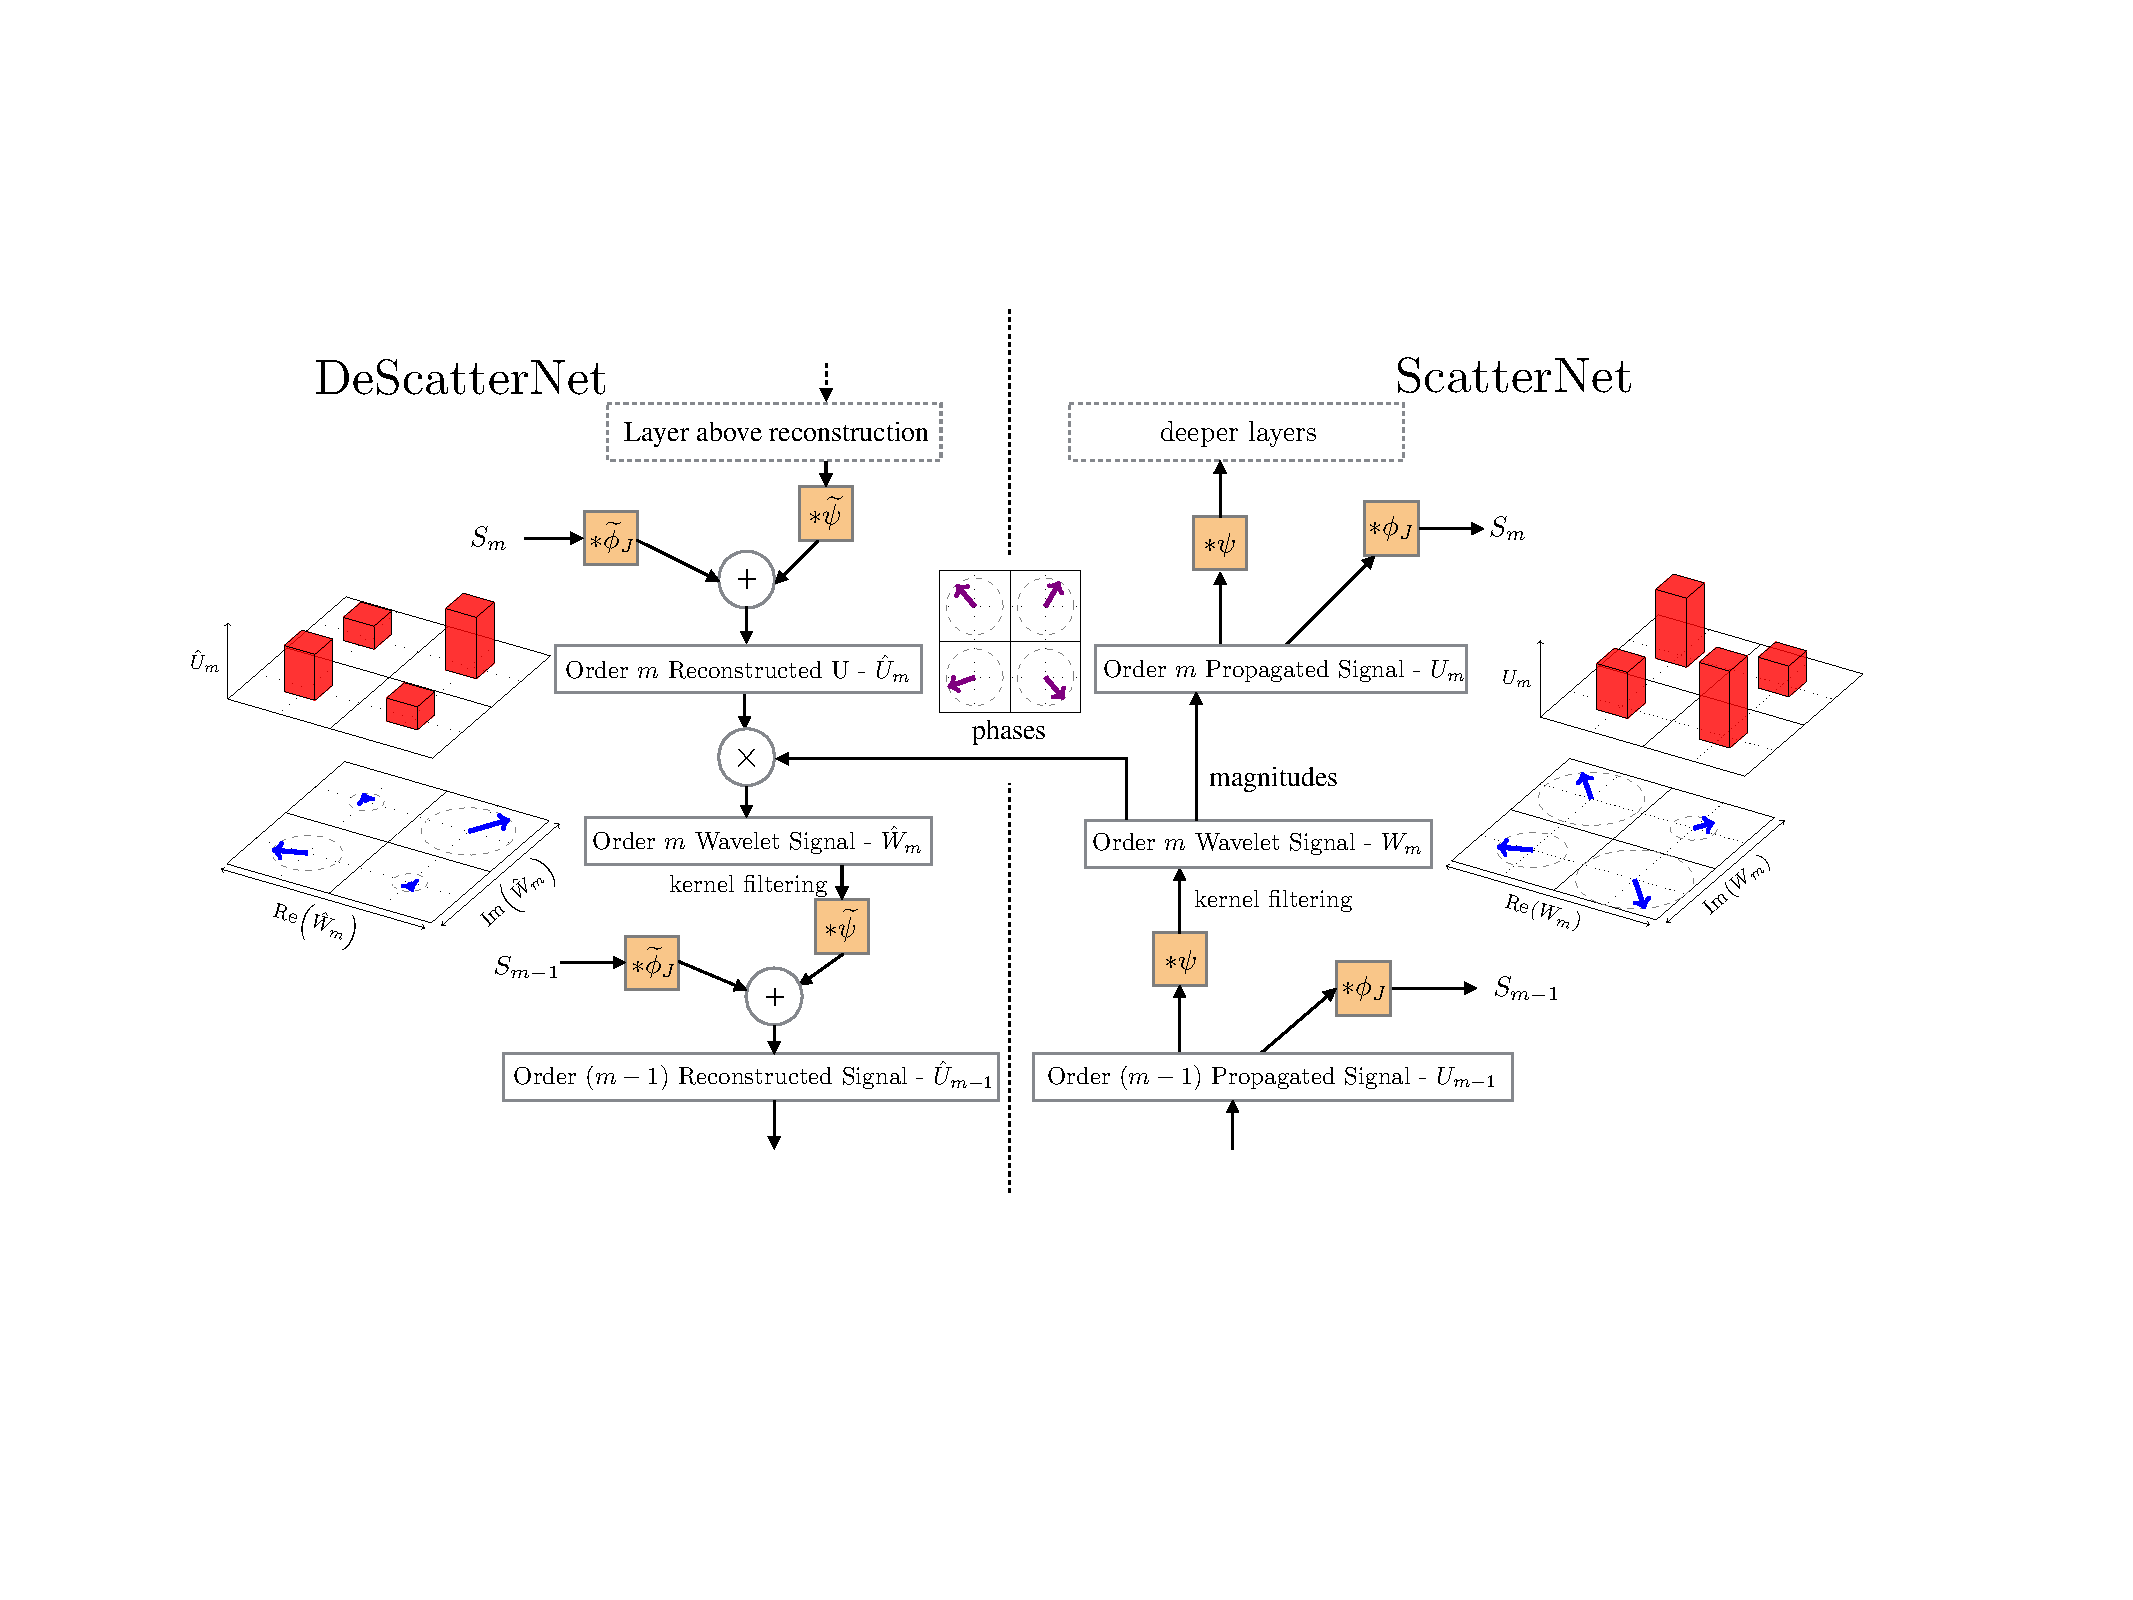
\includegraphics[width=\textwidth, trim={3cm 7cm 4cm 6cm},clip]{\imgpath/descat.pdf}
  \mycaption{The inverse scattering network}{Comprises a DeScattering layer (left)
  attached to a Scattering layer (right). We are using the same convention as
  \cite{zeiler_visualizing_2014} Figure 1 - i.e., the input signal starts in the
  bottom right-hand corner, passes forwards through the ScatterNet (up the right
  half), and then is reconstructed in the DeScatterNet (downwards on the left
  half). The DeScattering layer will reconstruct an approximate version of the
  previous order's propagated signal. The $2\x 2$ grids shown around the image
  are either Argand diagrams representing the magnitude and phase of small
  regions of \emph{complex} (De)ScatterNet coefficients or bar charts showing
  the magnitude of the \emph{real} (De)ScatterNet coefficients (after applying
  the modulus nonlinearity). For reconstruction, we need to save the discarded
  phase information and reintroduce it by multiplying it with the reconstructed
  magnitudes.}
  \label{fig:ch4:descat}
\end{figure}

We now introduce our inverse scattering network. This allows us to back-project
scattering coefficients to the image space; it is inspired by the
DeconvNet used by Zeiler and Fergus in
\cite{zeiler_visualizing_2014} to look into the deeper layers of CNNs. Like
the DeConvNet, the inverse scattering network is similar to backpropagating a
single strong activation (rather than the usual gradient terms).

We emphasize that instead of thinking about perfectly reconstructing $x$ from
$S\in \reals[C\x H'\x W']$, we want to see what signal/pattern in the input image caused
a large activation in each channel. This can then give us a good idea of what each
output channel is sensitive to, or what the ScatterNet is `extracting' from the input.
Note that we do not use any of the log normalization layers described in
\cite{oyallon_deep_2015, singh_dual-tree_2017}.

\subsection{Inverting the Low-Pass Filtering}
Going from the $U$ coefficients to the $S$ coefficients in the forward pass involves convolving by
a low pass filter $\phi_J$, possibly followed by decimation to make the output $(H\x
2^{-J})\x (W\x2^{-J})$.  $\phi_J$ is a purely real filter, and we can `invert'
this operation by interpolating $S$ to the same spatial size as $U$ and convolving with
the mirror image of $\phi_J$, $\widetilde{\phi}_J$ (this is equivalent to the
transpose convolution described in \cite{zeiler_visualizing_2014}).
\begin{equation}
  \label{eq:ch4:s_hat}
  \hat{S}_{m}x = (S_{m}x) \conv \widetilde{\phi}_J
\end{equation}
% This will not recover $U$ as it was on the forward pass, but will recover all
% the information in $U$ that caused a strong response in $S$.
We note that
interpolation usually involves lowpass smoothing of the signal, so this can all
be one operation.
% However this has
% the undesirable effect of creating multiple impulses in the next layer down's
% activations. When the next layer down is the image space this is not a problem,
% but when it is

\subsection{Inverting the Magnitude Operation}
In the same vein as \cite{zeiler_visualizing_2014}, we face a difficult
task in inverting the nonlinearity in our system.
% It has been proven that for
% particular wavelets, we can recover the phase from their modulus
% \cite{waldspurger_phase_2012}, but this is not a trivial operation. Instead, we
We lend inspiration from the switches introduced in the DeconvNet; the
switches in a DeconvNet save the location of maximal activations so that
on the backwards pass activation layers could be unpooled trivially. We do an
equivalent operation by saving the \emph{phase} of the complex activations.
On the backwards pass we reinsert the phase\footnote{We note that this is equivalent 
to finding the gradient through the magnitude operation, just as the `switches' 
from \cite{zeiler_visualizing_2014} are equivalent to taking the gradient of 
the max pooling layer.} to give our recovered $W$:
\begin{equation}
  \label{eq:ch4:w_hat}
  \hat{W}_{m}x = \left(\hat{U}_{m} x\right) e^{j\theta_{m}}
\end{equation}

\subsection{Inverting the Wavelet Decomposition}
Using the $\DTCWT$ makes inverting the wavelet transform simple, as we
can simply feed the coefficients through the synthesis filter banks to regenerate
the signal. For complex $\psi$, this is convolving with the conjugate transpose
$\widetilde{\psi}$:
\begin{eqnarray}
  \label{eq:ch4:x_hat}
  \hat{U}_{m-1}x &=& \hat{S}_{m-1}x + \hat{W}_{m}x \\
                 &=& (S_{m-1}x) \conv \widetilde{\phi}_J + \sum_{\lambda_m} \left(\hat{U}_m x\right) e^{j\theta_m}
  \conv \widetilde{\psi}_{\lambda_m}
\end{eqnarray}

\subsection{The $\DTCWT$ ScatterNet}
The combination of the above three stages can be repeated for higher orders. The
resulting DeScatterNet is shown in \autoref{fig:ch4:descat}.

For the $\DTCWT$ ScatterNet (from \autoref{alg:ch3:dtcwt_scat}), this is the same
as finding the \emph{gradient} from the corresponding channels in $Z$.

\section{Visualization with Inverse Scattering}
{
\renewcommand{\_}{\textscale{.6}{\textunderscore}}
\label{sec:ch4:visualization}

We scatter all of the images from ImageNet's validation set and record the top 9
images which most highly activate each of the $C$ channels in the ScatterNet.
This is the \emph{identification} phase (in which no inverse scattering is
performed).

Then, in the \emph{reconstruction} phase, we load in the $9\x C$ images and
scatter them one by one. We take the resulting 52 channel output vector and mask
all but the largest value in the channel we are currently
examining and mask all values in the other channels.
This 1-sparse tensor is then presented to the inverse scattering network from
\autoref{fig:ch4:descat} and projected back to the image space.

Some results of this are shown in \autoref{fig:ch4:reconstructions} for the
first and second-order coefficients. For a given output channel, we show the top
9 activations projected independently to pixel space. We also show the patch
of pixels in the input image which cause this large output. As there are 12
$S_1$ coefficients, we randomly choose 3 orientations from $S_1^1$ and 3 from $S_1^2$.
Similarly, there are 36 $S_2$ coefficients, so we randomly choose 16 of these.

The order 0 and order 1 scattering (labelled with `Order 1' in
\autoref{fig:ch4:reconstructions}) coefficients look quite similar to the first
layer filters from the well-known AlexNet CNN \cite{krizhevsky_imagenet_2012}.
This is not too surprising, as the first-order scattering coefficients are
simply a wavelet transform followed by average pooling. They are responding to
images with strong edges aligned with the wavelet orientation.

The second-order coefficients (labelled with `Order
2' in \autoref{fig:ch4:reconstructions}) appear very similar to the order
1 coefficients at first glance.
They too are sensitive to edge-like features, and some of them (e.g.\ third row,
third column and fourth row, second column) are mostly just that. These are
features that have the same oriented wavelet applied at both the first and
second-order ($\theta_1 = \theta_2$). Others, such as the nine in the top left
square (first row, first column), and top right square (first row, fourth
column) are more sensitive to checker-board like patterns. These are
activations where the orientation of the wavelet for the first and second-order
scattering were far from each other ($15\degs$ and $105\degs$ for the first row,
first column and $105\degs$ and $45\degs$ for the first row, fourth column).

For comparison, we include reconstructions from the second layer of the
well-known VGG CNN\@ (labelled with `VGG conv2\_2', in
\autoref{fig:ch4:reconstructions}). These were made with a DeconvNet, following the
same method as \cite{zeiler_visualizing_2014}. Note that while some of
the features are edge-like, we also see higher-order shapes like corners,
crosses and curves.

These reconstructions show that higher-order features from ScatterNets vary
significantly from those learned in CNNs. In many
respects, the features extracted from a CNN like VGGNet look preferable for use
as part of a classification system.
\begin{figure}[tp]
  \centering
  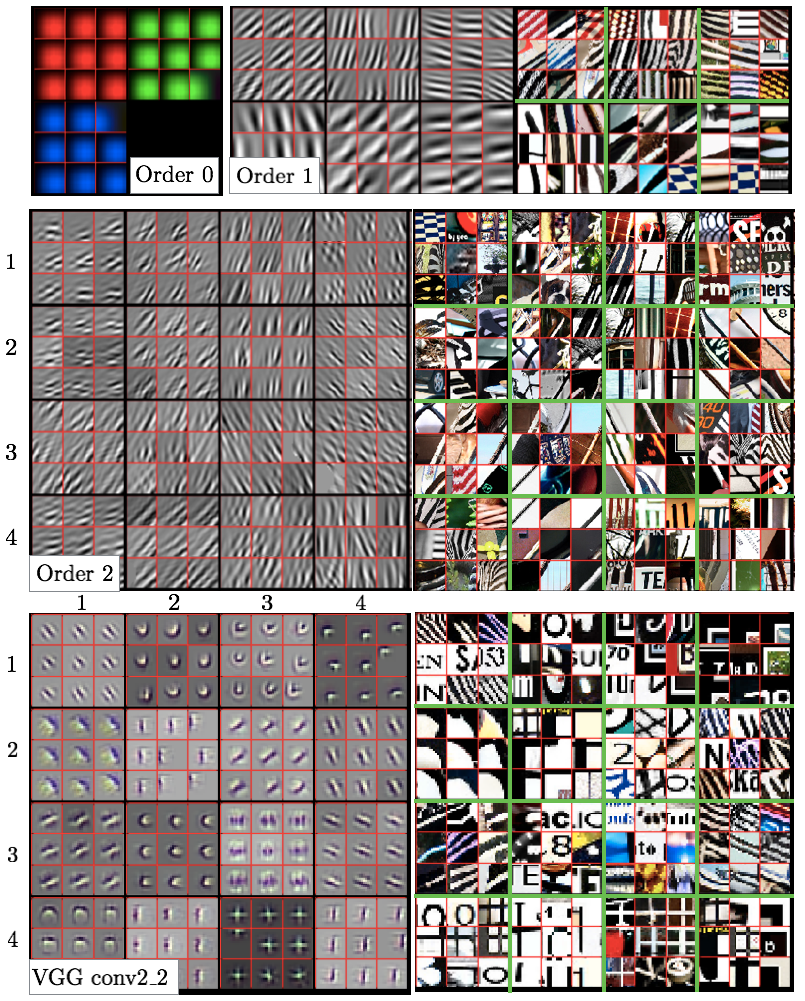
\includegraphics[width=0.9\textwidth]{\imgpath/deconv_images.png}
  \mycaption{Comparison of scattering to convolutional features}{Visualization
  of a random subset of features from $S_0$ (all 3), $S_1$ (6 from the 12) and
  $S_2$ (16 from the 36) scattering outputs. We record the top 9 activations for
  the chosen features and project them back to the pixel space. We show them
  alongside the input image patches which caused the large activations. We also
  include reconstructions from layer conv2\_2 of VGG Net
  \cite{simonyan_very_2014}(a popular CNN, often used for feature extraction)
  for reference --- here we display 16 of the 128 channels. The VGG
  reconstructions were made with a CNN DeconvNet based on
  \cite{zeiler_visualizing_2014}. Image best viewed digitally.}
  \label{fig:ch4:reconstructions}
\end{figure}

}

\chapter{Conclusion}\label{ch:conclusion}
\def \path {intro/}
\def \imgpath {intro/images}

In this thesis, we have examined the effectiveness of using complex wavelets as
basis functions for deep learning models. We summarize the key results we have
found before describing what we were not able to explore due to time constraints.

% We first looked at ScatterNets, a type
% of feature extractor that builds invariances using the complex magnitude
% operation, demodulating image energy towards zero. Having examined the
% properties of these ScThen we looked at a method
% that does not rely on demodulation, and simply learns complex gains for wavelet
% subbands. The input channels could then be mixed in a learned way much like a
% regular CNN convolutional layer. The first part of our research looked
% at ScatterNets as they were a promising starting point for achieving this task.

\section{Summary of Key Results}
\textbf{\Autoref{Chapter}{ch:dtcwt_scat}} shows how using the separable spatial implementation of 
the $\DTCWT$ as the chosen wavelets for the original ScatterNet design greatly
speeds up computation (see \autoref{tab:ch3:scat_speeds}). We were also able to
derive the backpropagation equations for wavelet and scattering layers, aiding
the use of ScatterNets as part of deep networks. As part of this, we tested out
the performance of the $\DTCWT$ based ScatterNet as a front end to a simple CNN for 
some small classification tasks, and compared its performance to the Morlet based system. We
found that as well as being faster, the performance was often better when using
the $\DTCWT$ wavelets \autoref{tab:ch3:comparison}. When doing these tests, we
found that of the wavelet choices available for the $\DTCWT$, those with the
fewest taps (and largest stopband gain and transition bandwidth) performed the best. This is
somewhat surprising and while we were not able to investigate why due to time
constraints, it may provide some interesting insights as to what the CNN backend 
is doing. It also may have been a side effect of the small image sizes used in the
classification task.

\textbf{\Autoref{Chapter}{ch:visualizing}} builds a visualization tool we call the
DeScatterNet. We use this to interrogate the input patches that most highly
excite the ScatterNet outputs on a subset of images from ImageNet (see
\autoref{fig:ch4:reconstructions}). We saw that
the second order scattering coefficients are most highly excited by ripple and
checkerboard like patterns. These were very different to the patters
that most highly excite filters of a CNN. We believe this may explain why
ScatterNets perform well on texture discrimination \cite{bruna_invariant_2013}
but less well on natural image classification \cite{oyallon_deep_2015}. We then
performed some occlusion tests on a hybrid network with a ScatterNet front end
and CNN backend and saw that the CNN was able to handle when the second
order scattering coefficients were zeroed out (there was only a small drop in
classification accuracy), but it suffered greatly when the zeroth or first order
coefficients were zeroed out. We also found the surprising result that on the
datasets we tested, diagonal edges were less important than their vertical or 
horizontal counterparts (\autoref{fig:ch4:occlusion1}). If the input images were
rotated by $\pm 30\degs$ then the diagonal channels became the most important.
This echoes the experiments of
\citeauthor{blakemore_development_1970}\cite{blakemore_development_1970} who
controlled the orinetation of edges exposed to kittens in their development
stage. Finally, this chapter showed some ways to expand on the ScatterNet
network\autoref{fig:ch4:newshapes}, inspiring the work of \autoref{ch:invariant}
and \autoref{ch:freqlearn}. This layer is \textbf{cheaper and quicker
theoretically?}

\textbf{\Autoref{Chapter}{ch:invariant}} reworks the ScatterNet into individual layers.
This redesign allows us to rethink how we want to use wavelets, and we introduce
the \emph{learnable ScatterNet} made up of \emph{locally invariant convolutional
layers}. Rather than applying the same layer twice to get a second order
ScatterNet, we introduce mixing across the output channels, taken after the
magnitude operation. The flexibility of the proposed layer means it can be used
in a ScatterNet-like system, where the number of output channels grows
exponentially with the number of layers, or in a CNN-like system, where the
number of output channels remains mostly constant across layers. We experimented
with both possibilities, showing that the extra learnability definitely helps
the ScatterNet style system (\autoref{tab:hybrid_scat}) and can help a CNN
(\autoref{tab:ch5:conv_results}). The demodulation of energy from the complex
modulus means that the proposed locally invariant layer can only be used a few
times. In particular, we saw that the layer performed best when used where a CNN
would naturally downsample (or pool) the input.

\textbf{\Autoref{Chapter}{ch:freqlearn}} looks at learning in the wavelet space without
taking complex magnitudes. We present the \emph{wavelet gain layer} which takes
inputs to the wavelet domain, learns complex gains to attenuate/accentuate
different subbands, mixes the subbands across the different channels and offers
the ability of returning to the pixel domain with the inverse wavelet transform.
We propose different possible nonlinearities to use in the wavelet domain and
found that while this was possible, it did not offer an advantage over learning
directly in the pixel domain (\autoref{fig:ch6:gl_results}). 

\section{Future Work}
This thesis has started to look at ways of using wavelets as basis functions for
deep learning models. Our research has found some possible ways they could be used
which offer some advantage in terms of number of parameters, interpretability
and (theoretical) computation time. But there are many things that we were not
able to try, and some of these may show that wavelets have a larger benefit than
we found.

\subsection{Faster Transforms and expanding current approaches}
Firstly, despite our best efforts in making a fast wavelet transform, the speed
of a $\DTCWT$ in \emph{Pytorch Wavelets} is slower than it could be. A $10\x 10$
convolutional filter with 100 multiplies per input pixel is roughly twice as
quick to compute as a $\DTCWT$ with 36 multiplies per pixel. We limited our
design to use high level cuDNN calls and this was the best we could do with
these primitives. We believe that any further speed up would require custom CUDA
kernels. The speed was not a problem for datasets such as CIFAR and Tiny
ImageNet, but it did prevent us from testing the wavelet gain layer and
invariant layer on ImageNet (see \autoref{app:arch} for some run times).
We believe that these layers may perform better with larger images.

Another aspect of testing larger images is the benefit of using multiple
scales in any system. Our wavelet gain layer only used the first or second scale
in our experiments, but the real benefit of decimated wavelet transforms is the
speedup they offer by allowing for multiscale approaches. Little research has
been done in splitting the input or mid-level activations into multiple scales
and learning different filters for the different scales, but some examples
include \cite{haber_learning_2017, fujieda_wavelet_2018}.

\subsection{Applications}
low dimensional medical applications
\cite{kang_deep_2017}

\subsection{ResNets and Lifting}
\begin{figure}
  \centering
  \subfloat[Residual]{
  \centering
  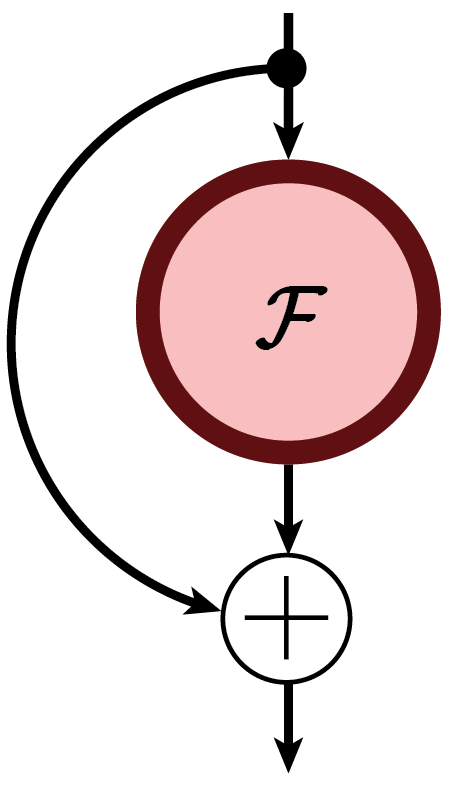
\includegraphics[width=0.13\textwidth]{\imgpath/resnet.png}
  }\qquad
  \subfloat[Lifting]{
  \centering
  \includegraphics[width=0.48\textwidth]{\imgpath/lifting.png}
  }
  \mycaption{Residual vs Lifting Layers}{In a residual layer, an input is
  transformed by a learned function $\mathcal{F}$ and added to itself. Typically
  $\norm{\mathcal{F}x} \ll \norm{x}$ meaning the vector $y$ is a small
  perturbation of the vector $x$. In a lifting layer, each path is a learned
  function of the other added to itself. In the original second generation
  wavelets, $\mathcal{F}$ and $\mathcal{G}$ are FIR filters, but there is no
  requirement on them to be.}
  \label{fig:ch7:lifting_resnet}
\end{figure}
We briefly mentioned ResNets in \autoref{sec:ch2:resnets} but did not study them
in depth in this thesis. Interestingly, there are many similarities between
ResNets and second generation wavelets, or the \emph{lifting} framework
\cite{sweldens_lifting_1998,daubechies_factoring_1998}.
In a residual layer, the output is $y = \mathcal{F}(x) + x$, for a lifting
system, the layer is a two port network:
\begin{align}
  y_1 &= \mathcal{F}(x_1) + x_2 \\
  y_2 &= \mathcal{G}(y_1) + x_1 
\end{align}
\autoref{fig:ch7:lifting_resnet} shows the similarities between the two designs. 
\cite{gomez_reversible_2017, jacobsen_i-revnet:_2018} both make the small modifications
to the ResNet design to make a lifting style architecture.
\cite{gomez_reversible_2017} do this to save memory on the activations for
backpropagation whereas \cite{jacobsen_i-revnet:_2018} use it for its perfect
reconstruction properties. We believe that there are potentially many more
benefits to using the lifting design as an extension of our work into learning
from basis functions.

In addition to the interesting parallel between ResNets and Lifting,
\citeauthor{bartlett_gradient_2018} have found that having near identity transforms
for each stage of a deep learning system is \cite{bartlett_gradient_2018, bartlett_representing_2018}
Aside from the interesting parallel between ResNets and Lifting, ResNets have
become 
\subsection{Protecting against Attacks}
\cite{cisse_parseval_2017}

\subsection{Convolutional Sparse Coding}

\cite{liu_online_2017, liu_first_2017, papyan_convolutional_2017}

\subsection{Energy Propagation and Weight Properties}
studying the energy propagation properties and singular values of layers

Miki Elad's work on CSC.

ResNets are really good. What was the paper on that?
(Bartlett




\chapter{A Learnable ScatterNet: Locally Invariant Convolutional Layers}

% Specify the path to this folder
\def \path {invariantlayer/}
\def \imgpath {invariantlayer/images}

The drive of this thesis is in exploring if complex wavelets (in
particular the $\DTCWT$) have any place in deep learning and if they do,
quantifying how beneficial they can be. The introduction of more powerful GPUs and
fast and popular deep learning frameworks such as PyTorch, Tensorflow and Caffe
in the past few years has helped the field of deep learning grow very rapidly.
Never before has it been so possible and so accessible to test new designs and
ideas for a machine learning algorithm than today. Despite this rapid growth,
there has been little interest in building wavelet analysis software in modern
frameworks.

This poses a challenge and an opportunity. To pave the way for more detailed
investigation (both in the rest of this thesis and by other researchers
who want to explore wavelets applied to deep learning), we must have the right
foundation and tools to facilitate research.

A good example of this is the current implementation of the ScatterNet. While
ScatterNets have been the most promising start in using wavelets in a deep
learning system, they have tended to be orders of magnitude slower, and significantly more
difficult to run than a standard convolutional network.

Additionally, any researchers wanting to explore the DWT in a deep learning
system have had to rewrite the filter bank implementation themselves, ensuring they
correctly handle boundary conditions and ensure correct filter tap alignment to
achieve perfect reconstruction.

\section{Chapter Layout}
This chapter describes how we have built a fast ScatterNet implementation in
PyTorch with the $\DTCWT$ as its wavelet transform. First, we describe how to do an
efficient DWT in PyTorch in \autoref{sec:ch3:dwt} before showing how to expand this
to an efficient $\DTCWT$ in \autoref{sec:ch3:dtcwt}.
We then use the $\DTCWT$ to define our own ScatterNet in \autoref{sec:ch3:scat} (in
particular, see \autoref{alg:ch3:dtcwt_scat}). 
All of the code is available as an open-source library at \emph{PyTorch Wavelets} \cite{cotter_pytorch_2018}.

In parallel with our efforts, the original authors of the ScatterNet have
improved their implementation, making a new package called KyMatIO\cite{andreux_kymatio:_2018}. 
We compare the speed and classification performance of our package to KyMatIO in \autoref{sec:ch3:comparison}
as this provides some interesting insights into the choice of complex wavelet
for a ScatterNet. This is similar to the work of
\cite{singh_multi-resolution_2016}, where
\citeauthor{singh_multi-resolution_2016} show that a $\DTCWT$-ScatterNet
outperforms a Morlet-ScatterNet when used as a front end to an
SVM for some simpler classification tasks.
We find that our proposed $\DTCWT$-ScatterNet is 7 to 15 times faster 
than KyMatIO (depending on the padding style and wavelet length), as well as
giving a small improvement in performance when used as a front end to a CNN.

% \chapter{Introduction}\label{ch:intro}

\def \path {other}
\def \imgpath {\path/images}

It has long been the goal of computer vision researchers to be able to develop
systems that can reliably recognize objects in a scene. Achieving this unlocks a huge
range of applications that can benefit society as a whole: fully
autonomous vehicles, automatic labelling of uploaded videos/images for
searching, interpretation and screening of security video feeds, and many more,
all far-reaching and extremely valuable. Many of these tasks are very tedious for humans
and would be done much better by machines if the missed-detection rate can be
kept low enough. The challenge does not lie in finding the
right application, but in the difficulty of training a computer to see.

Some of the difficulties associated with vision are the presence of nuisance
variables such as changes in lighting condition, changes in viewpoint, and
background clutter. These variables do not affect the scene but can drastically change the pixel
representation of it.
Humans, even at early stages of their lives, have little difficulty filtering
out these nuisance variables and are excellent at extracting the necessary information from a scene.
To design a robust system, it makes sense to take account of how our brains see
and understand scenes.

Unfortunately, biological vision is also a complex system. It has
more to it than simply collecting photons in the eye.
An excerpt from a recent Neurology paper \cite{raichle_two_2010} sums up the problem
well:

\begin{quotation}
It might surprise some to learn that visual information is significantly
degraded as it passes from the eye to the visual cortex. Thus, of the unlimited
information available from the environment, only about $10^{10}$ bits/sec are
deposited in the retina \ldots\ only $\sim 6\times 10^6$
bits/sec leave the retina and only $10^4$ make it to layer IV of V1
\cite{anderson_directed_2005,tor_norretranders_user_1998}. These data
clearly leave the impression that visual cortex receives an impoverished
representation of the world \ldots\ it should be noted that estimates of the
bandwidth of conscious awareness itself (i.e.,\ what we `see') are in the range
of 100 bits/sec or less\cite{anderson_directed_2005,
tor_norretranders_user_1998}.
\end{quotation}

Current video cameras somewhat act as a combination of the first and second
stage of this system, collecting photons in photosensitive sensors and then
converting this to a stream of images. Standard definition digital television
typically has
a bit rate between $3\x 10^6$ and $10^7$ bits/sec (slightly larger but comparable
to the $10^6$ bits/sec travelling through the optic nerve).

If we are to build effective vision systems, it makes sense to emulate this
compression of information between the optic nerve and the later stages of the visual
cortex. 
% The question now stands before us --- what information is kept on entry to the V1 cortex?
Hubel and Wiesel revolutionized our understanding of the V1 cortex in their Nobel prize-winning work
(awarded in 1981 in Physiology/Medicine) by
studying cats \cite{hubel_receptive_1959, hubel_receptive_1962}, macaques and spider
monkeys \cite{hubel_receptive_1968}. They found that neurons in the V1 cortex fired
most strongly when edges of a particular (i.e.,\ neuron-dependent) orientation
were presented to the animal, so long as the edge was inside the receptive field of
this neuron.
Continuing on this work, Blakemore and Cooper \cite{blakemore_development_1970}
analysed the perception of kittens that had restricted visual information
presented to them.
In one of their experiments, the kittens were kept in darkness
and then exposed for a few hours a day to only horizontal or vertical lines.
After five months, they were taken into natural environments and their reactions
were monitored. The two groups of cats would only play with objects when
presented in an orientation that matched the orientation of their original
environment. This suggest that these early layers of perception are
\emph{learned}.
% A figure of the the frequency response of the photoreceptor cells in our eyes
% to different wavelengths of light.
% \begin{figure}
  % \begin{center}
      % \includegraphics[width=10cm]{\imgpath/colour_sensitivity.jpg}
      % \mycaption{Frequency sensitivity of photoreceptors in they eye}
              % {Wavelength responsiveness of the different photoreceptors in the
               % eye. S, M, and L are short, medium, and long cones, compared to
               % R --- rods. Taken from~\cite{bowmaker_visual_1980}}
  % \end{center}
% \end{figure}

The current state of the art in image understanding systems are
Convolutional Neural Networks (CNNs). These are a learned model that
cascades many convolutional filters serially in layers, separated by
nonlinearities.
They are seemingly inspired by the visual cortex in the way that they are
hierarchically connected, progressively compressing the information into a
richer representation.

\autoref{fig:ch1:cnn_arch} shows an example CNN
architecture, the famous AlexNet \cite{krizhevsky_imagenet_2012}. Inputs are resized to a
manageable size, in this case, $224\x 224$ pixels. Multiple convolutional
filters of size $11\x 11$ are convolved over this input to give $96$ output
\emph{channels} (or \emph{activation maps}). In the figure, these are split onto two
graphics cards or GPUs for memory purposes. These are then passed through a
pointwise nonlinear function, or \emph{nonlinearity}.
The activations are pooled (a form of downsampling) and convolved with more
filters to give $256$ new channels at the second stage. This is repeated 3 more
times until the $13\x 13$ output with $256$ channels is unravelled and passed
through a fully connected neural network to classify the image as one of $1000$
possible classes.

CNNs have garnered lots of attention since 2012 when the previously mentioned AlexNet
nearly halved the top-5 classification error rate (from $26\%$ to $16\%$)
in the ImageNet Large Scale Visual Recognition Competition (ILSVRC)
\cite{russakovsky_imagenet_2014}\footnote{The previous state of
the art classifiers had been built by combining keypoint extractors like
SIFT\cite{lowe_distinctive_2004} and HOG\cite{dalal_histograms_2005} with
classifiers such as Support Vector Machines\cite{cortes_support-vector_1995} and
Fisher Vectors\cite{sanchez_image_2013}, for example \cite{sanchez_high-dimensional_2011}.}.
In the years since, the complexity of CNNs has grown significantly. AlexNet had
only 5 convolutional layers, whereas the 2015 ILSVRC winner ResNet \cite{he_deep_2016}
achieved 3.57\% top-5 error with 151 convolutional layers (and had some
experiments with 1000 layer networks).

\begin{figure}
  \centering
    % \includegraphics[width=\textwidth]{\imgpath/dtcwt_gain}
    \includegraphics[width=\textwidth]{\imgpath/alexnet.png}
    \mycaption{Convolutional Architecture example}{The previous layer's activations are
    combined with a learned convolutional filter.
    Note that while the activation maps are 3-D arrays, the convolution is only
    a 2-D operation. This means the filters have the same number of channels as
    the input and produce only one output channel. Multiple channels are made by
    convolving with multiple filters. Not shown here are the nonlinearities that
    happen in between convolution operations. Image taken from \cite{krizhevsky_imagenet_2012}.}
    \label{fig:ch1:cnn_arch}
  \end{figure}

\section{Motivation}\label{sec:ch1:motivation}
\begin{figure}
  \centering
  \subfloat[conv1 filters]{
  \includegraphics[width=0.6\textwidth]{\imgpath/alexfilters.png}
  \label{fig:ch1:alex_filt}
  }\\
  \subfloat[conv1 activations]{
  \includegraphics[width=\textwidth]{\imgpath/out1.jpg}
  \label{fig:ch1:alex_conv1}
  }\\
  \subfloat[conv2 activations]{
  \includegraphics[width=\textwidth]{\imgpath/out2.jpg}
  \label{fig:ch1:alex_conv2}
  }\\
  \subfloat[conv3 activations]{
  \includegraphics[width=\textwidth]{\imgpath/out3.jpg}
  \label{fig:ch1:alex_conv3}
  }
  \mycaption{Example first layer filters and the first three
  layer's outputs}{\subref{fig:ch1:alex_filt} The $11\x 11$ filters for the
  first stage of AlexNet. Of the 96 filters, 48 were learned on one GPU and
  another 48 on another GPU. Interestingly, one GPU has learned mostly
  lowpass/colour filters and the other has learned oriented bandpass
  filters. \subref{fig:ch1:alex_conv1} - \subref{fig:ch1:alex_conv3} Randomly
  chosen activations from the output of the first, second and third convolutional
  layers of AlexNet (see \autoref{fig:ch1:cnn_arch}) with negative values set to 0.
  Filters and activation images taken from supplementary material of
    \cite{krizhevsky_imagenet_2012}.}
  \label{fig:ch1:alexnet_filters}
\end{figure}

Despite their success, CNNs are often criticized for being \emph{black-box}
methods. You can view the first layer of filters
quite easily (see \autoref{fig:ch1:alex_filt}) as they exist in RGB
space, but beyond that things get trickier as the filters have a third, \emph{channel}
dimension, typically much larger than the two spatial dimensions. Additionally,
it is not clear what the input channels themselves correspond to. For illustration
purposes, we have also shown some example activations from the first three
convolutional layers for AlexNet in
\autoref{fig:ch1:alexnet_filters}\subref{fig:ch1:alex_conv1}-\subref{fig:ch1:alex_conv3}\footnote{These activations are
taken after a specific nonlinearity that sets negative values to 0, hence the
large black regions.}. For the conv1 activations in
\autoref{fig:ch1:alex_conv1}, we can accurately guess that some of the first layer
channels are responding to edges or colour information, but as we go deeper to
conv2 and conv3, it becomes less and less clear what each activation is
responding to.

This has started to become a problem, and while we are happy to trust modern
CNNs for isolated tasks, we are less likely to be comfortable with them driving
cars through crowded cities, or making executive decisions that affect people
directly. In a commonly used contrived example, it is not hard to imagine a deep
network that could be used to assess whether giving a bank loan to an applicant
is a safe investment. Trusting a black box solution is deeply unsatisfactory in
this situation. Not only from the customer's perspective, who, if declined, has
the right to know why \cite{goodman_european_2016}, but
also from the bank's --- before lending large sums of money, most banks
would like to know why the network has given the all clear. `It has worked well
before' is a poor rule to live by.

Aside from their lack of interpretability, it often takes a long time and a lot of
effort to train state-of-the-art CNNs. Typical networks that have won ILSVRC
since 2012 have had roughly 100 million parameters and take up to a week to train. This
is optimistic and assumes that you already know the necessary optimization or
architecture hyperparameters, which you often have to find out by trial and error.
In a conversation the author had with Yann LeCun, the attributed father of
CNNs, at a Computer Vision Summer School (ICVSS 2016), LeCun highlighted this problem
himself:
\begin{quote}
  There are certain recipes (for building CNNs) that work and certain recipes
  that don't, and we don't know why.
\end{quote}

Considering the recent success of CNNs, it is becoming more and more
important to understand \emph{how} and \emph{what} a network learns, so we can
interrogate what in the input has contributed to it making its classification or regression choice.
Without this information, the use of these incredibly powerful tools could be
restricted to research and proprietary applications.

\section{Approach}
The structure of convolutional layers is fairly crude in terms of signal
processing - arbitrary taps of an FIR filter are learned typically via
stochastic gradient descent from random starting states to minimize either a
mean-squared error or cross-entropy loss.

This leads us to ask a motivating question:
%
\begin{quote}
  Is it possible to learn convolutional filters as combinations of basis
  functions rather than individual filter taps?
\end{quote}

In achieving this, it is important to find ways to have an adequate
richness of filtering while reducing the number of parameters needed to specify resulting
filters. We want to contract the space of learning to a subspace or manifold that
is more useful. In much the same way, the convolutional layer in a CNN is a restricted
version of a fully connected layer in a multi-layer perceptron, yet adding this
restriction allowed us to train more powerful networks.

\begin{quote}
The intuition that we explore in this thesis is that \emph{complex wavelets} are
good basis functions for filtering in CNNs.
\end{quote}

\subsection{Why Complex Wavelets?}
Most modern approaches to CNNs are framed entirely in the spatial domain; our
choice of complex wavelets as the basis function to explore comes from the
deeper intuition that it may be helpful to rethink about CNNs in the
\emph{frequency domain}.  Historically, the frequency domain has been an
excellent space for solving many signal processing problems such as noise
removal, filter design, edge detection and data compression. We believe it may prove to
have advantages for CNNs too (beyond just an efficient space to do convolution
in).

The Fourier transform, which uses complex sinusoids as
its basis function, is perhaps the most ubiquitous tool to use for frequency
domain analysis. The problem with these complex sinusoids is that they have
\emph{infinite} support. This means that small changes in one part of an image
affect every Fourier coefficient. Additionally, they are not stable to small
deformations, as small changes can produce unbounded changes in the representation
\cite{mallat_group_2012}.

The common remedy to this problem is to use the localized, and more
stable, short-time Fourier transform (STFT). The STFT (or the Gabor transform)
is a natural extension of the Fourier transform, windowing the complex sinusoids
with a Gaussian (or similar) function. The STFT has the undesirable property that all
frequencies are sampled with the same resolution. A close relative of the STFT is the
continuous wavelet transform (CWT). The shorter duration of the wavelet basis
functions as the frequency increases means that their time resolving power
improves with centre-frequency.
Another commonly used
wavelet transform is the discrete wavelet transform (or the DWT) often favoured over
the CWT because of its speed of computation. It can use many
different finite support basis functions, all with different frequency
localization properties, but it is usually limited to using real filters. As such, it
suffers from many problems such as shift-dependence and lack of directionality in
two dimensions (2-D). These problems can be remedied by using the slower CWT with complex basis
functions, but we choose instead to use the dual-tree complex wavelet transform,
or $\DTCWT$ \cite{selesnick_dual-tree_2005} with q-shift filters \cite{kingsbury_complex_2001}.

The $\DTCWT$ allows for complex basis functions that have shift-invariance and
directionality, while being fast to implement like the DWT (in 2-D it can be thought of as the
application of 4 DWTs in parallel). It is also more easily invertible than the
CWT, forming a tight frame \cite{kovacevic_introduction_2008}, which we believe
may prove to be a very important property for visualizing what a
CNN is responding to.

We revisit the properties of the Fourier transform, STFT, CWT, DWT and $\DTCWT$
and expand on the properties behind our choice of basis functions
in the literature review \autoref{sec:ch2:fourier}.

On top of the intuition that the wavelet domain is a good space in which to frame CNNs,
there are some experimental motivating factors too. Firstly, the wavelet
transform has had much success in image and video compression, particularly for
JPEG2000 \cite{taubman_jpeg2000_2013}. Good compression performance implies an ability of
the basis functions to represent the input data sparsely (as seems to happen in
the brain). Secondly, the filters from the first layer of AlexNet
(\autoref{fig:ch1:alexnet_filters}) look like oriented wavelets. Given that
there was no prior placed on the filters to make them have this similarity to
wavelets, this result is noteworthy. And finally, the aforementioned work of
Hubel and Wiesel suggests that the early layers of the visual system act like a
Gabor transform.

These experimental observations imply that complex wavelets would do well in
replacing the first layer of a CNN, but we would aslo like to find out if they can be used
at deeper layers. Their well-understood and well-defined behaviour would help us
to answer the above \emph{how} and \emph{why} questions. Additionally, they
allow us to enforce a certain amount of smoothness and near orthogonality;
smoothness seems to be important to avoid sensitivity to adversarial or spoofing
attacks \cite{szegedy_intriguing_2014} and near orthogonality allows you to
cover a large space with fewer coefficients.

But first, we must find out \emph{if} it is possible to get the same or nearly the same
performance by using wavelets as the building blocks for CNNs, and this is the
core goal of this thesis.

\section{Method}
\subsection{ScatterNets}
To explore the uses of complex wavelets in CNNs, we begin by looking at one of the most
popular current uses of wavelets in image recognition tasks, the
Scattering Transform.

The Scattering Transform, or the \emph{ScatterNet}, was introduced in \cite{mallat_group_2012,
bruna_invariant_2013} at the same time as AlexNet. It is a non-black-box
network that can be thought of as a restricted complex-valued CNN
\cite{bruna_mathematical_2015}. Unlike a CNN, it has predefined
convolutional kernels, set to complex wavelet (and scaling) functions and uses
the complex magnitude as its nonlinearity. Due to
its well-defined structure, it can be analyzed and bounds on its stability to
shifts, noise and deformations are found in \cite{mallat_group_2012}.
%
% This is a promising start to addressing the problems of CNNs as using
% predefined, general filters helps us answer \emph{how} a CNN is
% learning, although the \emph{what} is still somewhat unclear.

For a simple task like identifying small handwritten digits,
the variabilities in the data are simple and small and the ScatterNet can easily
reduce the problem into a space which a Gaussian Support Vector Machine (or SVM
\cite{cortes_support-vector_1995}) can easily solve
\cite{bruna_invariant_2013}. For a more complex task like identifying real-world
objects, the ScatterNet can somewhat reduce the variabilities and get good
results with an SVM, but there is a significant performance gap between this and
what a CNN can achieve. For example, in \cite{oyallon_deep_2015} a second-order
ScatterNet can achieve $82.3\%$ top-1 classification accuracy on CIFAR-10, a
commonly used dataset, whereas modern CNNs such as \cite{he_deep_2016} can
achieve $93.4\%$.

\subsection{Learnable ScatterNets}
To start to address the performance gap between ScatterNet front ends and CNNs
we first investigate the properties of current ScatterNets. Inspired by the
visualization work of \citeauthor{zeiler_visualizing_2014}
\cite{zeiler_visualizing_2014} we build a DeScatterNet. The DeScatterNet
leverages the perfect reconstruction properties of the $\DTCWT$ and allows us to
investigate what in the input image the ScatterNet is responding to.

The DeScatterNet shows that the ScatterNet may be limiting itself by not
combining the filtering of different wavelet orientations (it does not mix the
channels as a CNN does). Inspired by the work of \cite{qiu_dcfnet:_2018}, we
propose the learnable ScatterNet, which includes this mixing while keeping the
desirable properties of the ScatterNet.

The learnable ScatterNet can be thought of as using the scattering outputs as
the \emph{basis functions}\footnote{Although they are not true basis functions
as they are the combination of a complex wavelet with a modulus nonlinearity,
and are thus data-dependent.} for our convolutional layers. We show that this
improves greatly on the ScatterNet design, and under certain constraints can
improve on the performance of CNNs too.

\subsection{Wavelet Domain Filtering}
We find that the complex modulus of the ScatterNet design to be useful for some
operations in a CNN, but it has a demodulating effect on the frequency energy
(all the outputs have significantly more energy in lower frequencies). This
limits repeated application of it as the demodulating effect compounds.

We develop a system that does not use the complex modulus; instead, it
learns \emph{complex} gains in the wavelet domain.
Rather than mixing subbands together, we keep them independent and only learn to
mix across the channel dimension. This is important, as it allows us to then use the inverse
$\DTCWT$ to return to the pixel domain. The shift-invariant properties of the $\DTCWT$ mean the
reconstructed outputs are (mostly) free from aliasing effects, despite much of
the processing being carried out at significantly reduced sample rates in the
wavelet domain.

We show that our layer can be used alongside regular convolutional
layers. I.e., it becomes possible to `step' into the wavelet domain to do
wavelet filtering for one layer, before `stepping' back into the pixel domain to
do pixel filtering for the next layer.

\section{Thesis Layout and Contributions to Knowledge}
This thesis has one literature review chapter and four novel-work chapters:
\begin{itemize}
\item
  \hyperref[ch:litreview]{Chapter~\ref*{ch:litreview}}
  explores some of the background necessary for starting
  to develop image understanding models. In particular, it covers the
  inspiration for CNNs and the workings of CNNs themselves, as well as covering
  the basics of wavelets and ScatterNets.
\item
  \Autoref{Chapter}{ch:dtcwt_scat} proposes a change to the core of the ScatterNet. In
  addition to performance issues with ScatterNets, they are slow and both
  memory-intensive and compute-intensive to calculate. This in itself is enough of an
  issue to make it unlikely that they would be used as part of deep networks. To
  overcome this, we change the computation to use the $\DTCWT$
  \cite{selesnick_dual-tree_2005} instead of Morlet wavelets, achieving a 20 to
  30 times speed-up while achieving a small improvement in classification performance.
\item
  \Autoref{Chapter}{ch:visualizing} describes our \emph{DeScatterNet}, a tool used to
  interrogate the structure of ScatterNets. We also perform tests to determine
  the usefulness of the different scattered outputs finding that many of them
  are not useful for image classification.
\item
  \Autoref{Chapter}{ch:invariant} describes the \emph{Learnable ScatterNet} we have developed to
  address some of the issues found from the interrogation in
  \autoref{ch:visualizing}. We find that a learnable ScatterNet layer performs
  better than a regular ScatterNet, and can improve on the performance of a CNN
  if used instead of pooling layers. We also find that scattering works well not
  just on RGB images, but can also be useful when used after one layer of
  learning.
\item
  In \autoref{ch:freqlearn}, we step away from ScatterNets and present the
  \emph{Wavelet Gain Layer}. The gain layer uses
  the wavelet space as a latent space to learn representations. We find possible
  nonlinearities and describe how to learn in both the pixel and wavelet domain.
  This work showed that there may well be benefits to learning in the wavelet
  domain for earlier layers of CNNs, but we have not yet found advantages to
  using the wavelet gain layer for deeper layers.
\end{itemize}

\subsection{Contributions and Publications}
The key contributions of this thesis are:

\begin{itemize}
  \item Software for wavelets and $\DTCWT$ based ScatterNet (described in \autoref{ch:dtcwt_scat})
    and publicly available at \cite{cotter_pytorch_2018}.
  \item ScatterNet analysis and visualizations (described in
    \autoref{ch:visualizing}). This chapter expands on the paper we presented at MLSP2017
    \cite{cotter_visualizing_2017}.
  \item Invariant Layer/Learnable ScatterNet (described in \autoref{ch:invariant})). This chapter expands
    on the paper accepted at ICIP2019 \cite{cotter_learnable_2019}. Software
    available at \cite{cotter_learnable_2019-1}.
  \item Learning convolutions in the wavelet domain (described in
    \autoref{ch:freqlearn}). We have published preliminary results on this work
    to arXiv \cite{cotter_deep_2018} but have expanded on this paper in the
    chapter. Software available at \cite{cotter_dtcwt_2018}.
\end{itemize}

\subsection{Related Research}
Readers may also be interested in the theses \cite{singh_scatternet_2018} and
\cite{oyallon_analyzing_2017}.

In \cite{singh_scatternet_2018}
\citeauthor{singh_scatternet_2018} looks at using the ScatterNet as a fixed
front end and combining it with well-known machine learning methods such as
SVMs, Autoencoders and Restricted Boltzmann Machines. By combining frameworks in
a defined way he creates unsupervised feature extractors which can then be used
with simple classifiers. Some relevant papers that makeup this thesis are \cite{singh_multi-resolution_2016,
singh_scatternet_2017, singh_generative_2018}. In
\cite{singh_multi-resolution_2016} Singh shows
that the $\DTCWT$-ScatterNet outperforms a Morlet-ScatterNet when used as a front end for
an SVM, which is similar to the work we do in \autoref{ch:dtcwt_scat} where we
show the $\DTCWT$-ScatterNet outperforms a Morlet-ScatterNet when used as a
front end for CNNs. He then expands on this work by testing other backends in
\cite{singh_scatternet_2017, singh_generative_2018}.

In \cite{oyallon_analyzing_2017}
\citeauthor{oyallon_analyzing_2017} looks at ScatterNets as front ends to
deeper learning systems, such as CNNs. Some relevant papers that makeup Oyallon's thesis are
\cite{oyallon_deep_2015, oyallon_scaling_2017, oyallon_hybrid_2017}. \cite{oyallon_scaling_2017, oyallon_hybrid_2017}
are particularly relevant as he uses a ScatterNet as a feature extractor for a
CNN. We do similar research in \autoref{ch:invariant}, but allow for
learned weights in the ScatterNet in our design.

\section{Related Work}\label{sec:ch5:related}

There have been several similar works that look into designing new convolutional
layers by separating them into two stages --- a first stage that performs a
non-standard filtering process, and a second stage that combines the first stage
into single activations. The inception layer 
\cite{szegedy_rethinking_2015} by \citeauthor*{szegedy_rethinking_2015} does this by filtering with different
kernel sizes in the first stage, and then combining with a $1\x 1$ convolution
in the second stage. \citeauthor*{ioannou_training_2015} also do something similar by making
a first stage with horizontal and vertical filters, and then combining in the
second stage again with a $1\x 1$ convolution\cite{ioannou_training_2015}. But perhaps the most similar
works are those that use a first stage with fixed filters, combining them in a
learned way in the second stage. Of particular note are:
\begin{itemize}
\item 
\citetitle{juefei-xu_local_2016} \cite{juefei-xu_local_2016}. This paper builds a
first stage with a small $3\x 3$ kernel filled with zeros, and randomly insert
$\pm 1$ in several locations, keeping a set sparsity level. This builds a very
crude spatial differentiator in random directions. The output of the first stage
is then passed through a sigmoid nonlinearity before being mixed with a $1\x 1$
convolution. The imposed structure on the first stage was found to be a good
regularizer and prevented overfitting, and the combination of the mixing in the
second layer allowed for a powerful and expressive layer, with performance near
that of a regular CNN layer.

\item
``DCFNet: Deep Neural Network with Decomposed Convolutional Filters"
\cite{qiu_dcfnet:_2018}. This paper decomposes convolutional filters as linear
combinations of Fourier Bessel and random bases.  The first stage projects the
inputs onto the chosen basis, and the second stage learns how to mix these
projections with a $1\x 1$ convolution. Unlike \cite{juefei-xu_local_2016} this
layer is purely linear. The supposed advantage being that the
basis can be truncated to save parameters and make the input less susceptible to
high frequency variations. The work found that this layer had marginal benefits
over regular CNN layers in classification, but had improved stability to noisy
inputs. 

\end{itemize}

\section{Recap of Useful Terms}\label{sec:ch5:background}

\subsection{Convolutional Layers}\label{sec:ch5:conv}

Let the output of a CNN at layer $l$ be 
$ \cnnlact{x}{l}{c}{\xy}, \quad c\in \{0, \ldots C_l-1\}, \xy \in \reals[2]$
where $c$ indexes the channel dimension, and $\xy$ is a vector of coordinates
for the spatial position. Of course, $\xy$ is typically sampled on a grid, but
we keep it continuous to more easily differentiate between the spatial and
channel dimensions. Recall from \eqref{eq:ch2:conv4} and \eqref{eq:ch2:conv4a} that
a convolutional layer in a standard CNN is defined by the two operations:
%
\begin{eqnarray} 
  \cnnlact{y}{l+1}{f}{\xy} &=& \sum_{c=0}^{C_l - 1}  x^{(l)}(c,\xy) \conv h^{(l)}_{f}(c, \xy)
    \label{eq:ch5:conv}\\
    \cnnlact{x}{l+1}{f}{\xy} & = & \sigma \left( \cnnlact{y}{l+1}{f}{\xy} \right) \label{eq:ch5:nonlin}
\end{eqnarray}

where $\cnnfilt{l}{f}{c}{\xy}$ is the $f$th filter of the $l$th layer with $C_l$
different point spread functions, and $f \in \{0, \ldots, C_{l+1}-1 \}$. $\sigma$ is a nonlinearity 
such as the ReLU, possibly combined with scaling such as batch normalization. The convolution
is done independently for each $c$ in the $C_l$ channels and the resulting outputs are
summed together to give one activation map. 

\subsection{Wavelet Transforms}\label{sec:ch5:wavelets}
Recall from \eqref{eq:ch2:wave2} that:
\begin{equation}
  \mathcal{W}x(c, \xy) = \left\{x(c, \xy) \ast \phitd_J(\xy),\ x(c, \xy) \ast \psitd_{\lambda}(\xy) \right\}_{\lambda} \label{eq:ch5:wave2}
\end{equation}
Where $\psitd_\lambda$ is a mother wavelet dilated by $2^j,\ 1 \leq j \leq J$ and rotated by
$\theta = \frac{\pi + 2k\pi}{12},\ 0\leq k < 6$:
%
\begin{equation}
  \psi_{j, \theta}(\xy) = 2^{-j}\psi \left(2^{-j} r_{-\theta} \xy\right)
\end{equation}
Define the set of all possible $\lambda$s as $\Lambda$ whose size is $|\Lambda | = JK$.
%
\subsection{Scattering Transforms}\label{sec:ch5:scatter}
As the real and imaginary parts of complex wavelets are in quadrature with
each other, taking the modulus of the resulting transformed coefficients removes
the high frequency oscillations of the output signal while preserving the energy
of the coefficients over the frequency band covered by $\psi_\lambda$. This is
crucial to ensure that the scattering energy is concentrated towards
zero-frequency as the scattering order increases, allowing sub-sampling.
% We experimentally show in \autoref{sec:??} that it plays a vital role in the
%classification process. 
We define the wavelet modulus propagator to be:
%
\begin{equation}
  \label{eq:ch5:wave_mod}
\widetilde{\mathcal{W}}x(c, \xy) = \left\{ x(c, \xy) \conv \phi_{J}(\xy),\ |x(c, \xy) \conv \psi_\lambda (\xy) | \right\}_{\lambda \in \Lambda} 
\end{equation}
The modulus terms are called $U[\lambda] x = \lvert x \conv \psi_\lambda \rvert$, and the scattering terms
are $S[\lambda] x = U[\lambda]x \conv \phi_J (\xy)$.

\section{The Scattering Transform} \label{sec:ch4:scatternet}
While we have introduced the scattering transform before, we clarify the format
we use for this chapter's analysis.

We use the $\DTCWT$ based ScatterNet introduced in the previous chapter --
\autoref{alg:ch3:dtcwt_scat} as a front end, with $K=6$ orientations, $J=2$
scales and $M=2$ orders.

Consider a single-channel input signal $x(\xy)$, $\xy \in \reals[2]$.
The zeroth-order scatter coefficient is the lowpass output of a $J$
level filter bank:
%
\begin{equation}
  S_0x(\xy) \definedas x(\xy) \conv \phi_J(\xy)
\end{equation}
%
This is approximately invariant to translations of up to $2^J$ pixels\footnote{From here on,
we drop the $\xy$ notation when indexing $x$, for clarity.}. In exchange for
gaining invariance, the $S_0$ coefficients have lost information
(contained in the rest of the frequency space). The remaining energy of $x$ is
contained within the first-order \emph{wavelet} coefficients:
\begin{equation}
  W_1x(\lambda_1, \xy) \definedas x \conv \psi_{\lambda_1}
\end{equation}
for $\lambda_1 = (j_1, \theta_1)$, $j_1\in\{1, 2\}, \theta_1 = \frac{\pi +
2k\pi}{12}$ with $k \in \{0, 1, \ldots 5\}$.

Taking the magnitude of $W_1$ gives us the first-order \emph{propagated}
signals:
\begin{equation}
  U_1x(\lambda_1, \xy) \definedas |x \conv \psi_{\lambda_1}|
    = \sqrt{(x \conv \psi^r_{\lambda_1})^2 + (x \conv \psi^i_{\lambda_1})^2}
\end{equation}
The first-order scattering coefficient make $U_1$ invariant up to
the coarsest scale $J$ by averaging it:
\begin{equation}
  S_1x(\lambda_1, \xy) \definedas |x \conv \psi_{\lambda_1}| \conv \phi_J
\end{equation}
This has $KJ = 6\x 2 = 12$ output channels for each input channel. Later in this
chapter we will want to distinguish between the first and second scale
coefficients of the $S_1$ terms, which we will do by moving the $j$ index
to a superscript. I.e., $S_1^1$ and $S_1^2$ refer to the set of 6 $S_1$ terms
at the first and second scales.

The second-order scattering coefficients are defined only on paths of
decreasing frequency (i.e. $J_2 < J_{1}$) \cite{bruna_invariant_2013}
\begin{equation}
  S_2x(\lambda_1, \lambda_2, \xy) \definedas |U_1x \conv \psi_{\lambda_2}| \conv \phi_J \label{eq:ch4:s2}
\end{equation}
Previous work shows that for natural images we get diminishing returns after
$m=2$. Our output is then a stack of these 3 outputs:
\begin{equation}
  Sx = \{S_0x, S_1x, S_2x\}
\end{equation}
with $1+12+36=49$ channels per input channel.

\subsection{Scattering Colour Images}\label{sec:ch4:colour}
A wavelet transform like the $\DTCWT$ accepts single-channel input yet we
often work on RGB images. This leaves us with a choice. We can either:
\begin{enumerate}
  \item Apply the wavelet transform (and the subsequent scattering operations)
    on each channel independently. This would triple the output size to $3C$.
  \item Define a frequency threshold below which we keep colour information, and
    above which, we combine the three channels.
\end{enumerate}
The second option uses the well known fact that the human eye is far less sensitive
to higher spatial frequencies in colour channels than in luminance channels.
This also fits in with the first layer filters seen in the well known
Convolutional Neural Network, AlexNet. Roughly one half of the filters were low
frequency colour `blobs', while the other half were higher frequency, greyscale,
oriented wavelets.

For this reason, we choose the second option for the
architecture described in this chapter. We keep the 3 colour
channels in our $S_0$ coefficients but work only on greyscale for high orders
(the $S_0$ coefficients are the lowpass bands of a J-scale wavelet transform, so
we have effectively chosen a colour cut-off frequency of $2^{-J} \frac{f_s}{2}$).

We combine the three channels by modifying our magnitude operation from \eqref{eq:ch3:magbias}
to now be:
\begin{equation}\label{eq:ch4:colour_mag}
 r_s = \sqrt{x_r^2 + y_r^2 + x_g^2 + y_g^2 + x_b^2 + y_b^2 + b^2} - b
\end{equation}
Where $x_r, x_g, x_b$ are the real parts of the wavelet response for the red,
green and blue channels, and $y$ is the corresponding imaginary part. This only
affects the $S_1$ coefficients and the $S_2$ coefficients then are calculated
as per \eqref{eq:ch4:s2}.

An alternative to \eqref{eq:ch4:colour_mag} is to combine the colours
\emph{before} scattering into a luminance channel. However, we choose to use \eqref{eq:ch4:colour_mag}
instead as this has the ability to detect colour edges with constant luminance.

With $J=2$ the resulting scattering output now has $3 + 12 + 36 = 51$ channels at $1/16$ the
spatial input size.

\section{The Inverse Scatter Network}\label{sec:ch4:descatternet}
\begin{figure}[t]
  \centering
  \includegraphics[width=\textwidth, trim={3cm 7cm 4cm 6cm},clip]{\imgpath/descat.pdf}
  \mycaption{The inverse scattering network}{Comprises a DeScattering layer (left)
  attached to a Scattering layer (right). We are using the same convention as
  \cite{zeiler_visualizing_2014} Figure 1 - i.e., the input signal starts in the
  bottom right-hand corner, passes forwards through the ScatterNet (up the right
  half), and then is reconstructed in the DeScatterNet (downwards on the left
  half). The DeScattering layer will reconstruct an approximate version of the
  previous order's propagated signal. The $2\x 2$ grids shown around the image
  are either Argand diagrams representing the magnitude and phase of small
  regions of \emph{complex} (De)ScatterNet coefficients or bar charts showing
  the magnitude of the \emph{real} (De)ScatterNet coefficients (after applying
  the modulus nonlinearity). For reconstruction, we need to save the discarded
  phase information and reintroduce it by multiplying it with the reconstructed
  magnitudes.}
  \label{fig:ch4:descat}
\end{figure}

We now introduce our inverse scattering network. This allows us to back-project
scattering coefficients to the image space; it is inspired by the
DeconvNet used by Zeiler and Fergus in
\cite{zeiler_visualizing_2014} to look into the deeper layers of CNNs. Like
the DeConvNet, the inverse scattering network is similar to backpropagating a
single strong activation (rather than the usual gradient terms).

We emphasize that instead of thinking about perfectly reconstructing $x$ from
$S\in \reals[C\x H'\x W']$, we want to see what signal/pattern in the input image caused
a large activation in each channel. This can then give us a good idea of what each
output channel is sensitive to, or what the ScatterNet is `extracting' from the input.
Note that we do not use any of the log normalization layers described in
\cite{oyallon_deep_2015, singh_dual-tree_2017}.

\subsection{Inverting the Low-Pass Filtering}
Going from the $U$ coefficients to the $S$ coefficients in the forward pass involves convolving by
a low pass filter $\phi_J$, possibly followed by decimation to make the output $(H\x
2^{-J})\x (W\x2^{-J})$.  $\phi_J$ is a purely real filter, and we can `invert'
this operation by interpolating $S$ to the same spatial size as $U$ and convolving with
the mirror image of $\phi_J$, $\widetilde{\phi}_J$ (this is equivalent to the
transpose convolution described in \cite{zeiler_visualizing_2014}).
\begin{equation}
  \label{eq:ch4:s_hat}
  \hat{S}_{m}x = (S_{m}x) \conv \widetilde{\phi}_J
\end{equation}
% This will not recover $U$ as it was on the forward pass, but will recover all
% the information in $U$ that caused a strong response in $S$.
We note that
interpolation usually involves lowpass smoothing of the signal, so this can all
be one operation.
% However this has
% the undesirable effect of creating multiple impulses in the next layer down's
% activations. When the next layer down is the image space this is not a problem,
% but when it is

\subsection{Inverting the Magnitude Operation}
In the same vein as \cite{zeiler_visualizing_2014}, we face a difficult
task in inverting the nonlinearity in our system.
% It has been proven that for
% particular wavelets, we can recover the phase from their modulus
% \cite{waldspurger_phase_2012}, but this is not a trivial operation. Instead, we
We lend inspiration from the switches introduced in the DeconvNet; the
switches in a DeconvNet save the location of maximal activations so that
on the backwards pass activation layers could be unpooled trivially. We do an
equivalent operation by saving the \emph{phase} of the complex activations.
On the backwards pass we reinsert the phase\footnote{We note that this is equivalent 
to finding the gradient through the magnitude operation, just as the `switches' 
from \cite{zeiler_visualizing_2014} are equivalent to taking the gradient of 
the max pooling layer.} to give our recovered $W$:
\begin{equation}
  \label{eq:ch4:w_hat}
  \hat{W}_{m}x = \left(\hat{U}_{m} x\right) e^{j\theta_{m}}
\end{equation}

\subsection{Inverting the Wavelet Decomposition}
Using the $\DTCWT$ makes inverting the wavelet transform simple, as we
can simply feed the coefficients through the synthesis filter banks to regenerate
the signal. For complex $\psi$, this is convolving with the conjugate transpose
$\widetilde{\psi}$:
\begin{eqnarray}
  \label{eq:ch4:x_hat}
  \hat{U}_{m-1}x &=& \hat{S}_{m-1}x + \hat{W}_{m}x \\
                 &=& (S_{m-1}x) \conv \widetilde{\phi}_J + \sum_{\lambda_m} \left(\hat{U}_m x\right) e^{j\theta_m}
  \conv \widetilde{\psi}_{\lambda_m}
\end{eqnarray}

\subsection{The $\DTCWT$ ScatterNet}
The combination of the above three stages can be repeated for higher orders. The
resulting DeScatterNet is shown in \autoref{fig:ch4:descat}.

For the $\DTCWT$ ScatterNet (from \autoref{alg:ch3:dtcwt_scat}), this is the same
as finding the \emph{gradient} from the corresponding channels in $Z$.

\section{Visualization with Inverse Scattering}
{
\renewcommand{\_}{\textscale{.6}{\textunderscore}}
\label{sec:ch4:visualization}

We scatter all of the images from ImageNet's validation set and record the top 9
images which most highly activate each of the $C$ channels in the ScatterNet.
This is the \emph{identification} phase (in which no inverse scattering is
performed).

Then, in the \emph{reconstruction} phase, we load in the $9\x C$ images and
scatter them one by one. We take the resulting 52 channel output vector and mask
all but the largest value in the channel we are currently
examining and mask all values in the other channels.
This 1-sparse tensor is then presented to the inverse scattering network from
\autoref{fig:ch4:descat} and projected back to the image space.

Some results of this are shown in \autoref{fig:ch4:reconstructions} for the
first and second-order coefficients. For a given output channel, we show the top
9 activations projected independently to pixel space. We also show the patch
of pixels in the input image which cause this large output. As there are 12
$S_1$ coefficients, we randomly choose 3 orientations from $S_1^1$ and 3 from $S_1^2$.
Similarly, there are 36 $S_2$ coefficients, so we randomly choose 16 of these.

The order 0 and order 1 scattering (labelled with `Order 1' in
\autoref{fig:ch4:reconstructions}) coefficients look quite similar to the first
layer filters from the well-known AlexNet CNN \cite{krizhevsky_imagenet_2012}.
This is not too surprising, as the first-order scattering coefficients are
simply a wavelet transform followed by average pooling. They are responding to
images with strong edges aligned with the wavelet orientation.

The second-order coefficients (labelled with `Order
2' in \autoref{fig:ch4:reconstructions}) appear very similar to the order
1 coefficients at first glance.
They too are sensitive to edge-like features, and some of them (e.g.\ third row,
third column and fourth row, second column) are mostly just that. These are
features that have the same oriented wavelet applied at both the first and
second-order ($\theta_1 = \theta_2$). Others, such as the nine in the top left
square (first row, first column), and top right square (first row, fourth
column) are more sensitive to checker-board like patterns. These are
activations where the orientation of the wavelet for the first and second-order
scattering were far from each other ($15\degs$ and $105\degs$ for the first row,
first column and $105\degs$ and $45\degs$ for the first row, fourth column).

For comparison, we include reconstructions from the second layer of the
well-known VGG CNN\@ (labelled with `VGG conv2\_2', in
\autoref{fig:ch4:reconstructions}). These were made with a DeconvNet, following the
same method as \cite{zeiler_visualizing_2014}. Note that while some of
the features are edge-like, we also see higher-order shapes like corners,
crosses and curves.

These reconstructions show that higher-order features from ScatterNets vary
significantly from those learned in CNNs. In many
respects, the features extracted from a CNN like VGGNet look preferable for use
as part of a classification system.
\begin{figure}[tp]
  \centering
  \includegraphics[width=0.9\textwidth]{\imgpath/deconv_images.png}
  \mycaption{Comparison of scattering to convolutional features}{Visualization
  of a random subset of features from $S_0$ (all 3), $S_1$ (6 from the 12) and
  $S_2$ (16 from the 36) scattering outputs. We record the top 9 activations for
  the chosen features and project them back to the pixel space. We show them
  alongside the input image patches which caused the large activations. We also
  include reconstructions from layer conv2\_2 of VGG Net
  \cite{simonyan_very_2014}(a popular CNN, often used for feature extraction)
  for reference --- here we display 16 of the 128 channels. The VGG
  reconstructions were made with a CNN DeconvNet based on
  \cite{zeiler_visualizing_2014}. Image best viewed digitally.}
  \label{fig:ch4:reconstructions}
\end{figure}

}

\section{Implementation Details}\label{sec:implementation}
Again, we use the $\DTCWT$ \cite{selesnick_dual-tree_2005} for our wavelet filters
$\psi_{j, \theta}$ due to their fast implementation with separable convolutions
which we will discuss more in \autoref{sec:computation}.  There are two side
effects of this choice. The first is that the number of orientations of wavelets
is restricted to $K=6$. The second is that we naturally downsample the output
activations by a factor of $2$ for each direction for each scale $j$, giving a 
$4^j$ downsampling factor overall. This represents the
source of the invariance in our layer. If we do not wish to downsample the
output (say to make the layer fit in a larger network), we can bilinearly
interpolate the output of our layer. This is computationally cheap to do on its
own, but causes the next layer's computation to be higher than necessary (there
will be almost no energy for frequencies higher than $f_s/4$).

In all our experiments we set $J=1$ for each invariant layer,
meaning we can mix the lowpass and bandpass coefficients at the same resolution.
\autoref{fig:block_diagram} shows how this is done. Note that setting $J=1$ for
a single layer does not restrict us from having $J>1$ for the entire system, as
if we have a second layer with $J=1$ after the first, including downsampling
($\downarrow$), we would have:
%
\begin{equation}
  \left(\left(\left(x \conv \phi_1\right) \downarrow 2\right) \conv \psi_{1, \theta}\right) 
    \downarrow 2 = \left(x \conv \psi_{2, \theta}\right) \downarrow 4
\end{equation}

\subsection{Parameter Memory Cost}\label{sec:memory}
A standard convolutional layer with $C_l$ input channels, $C_{l+1}$ output channels
and kernel size $L\x L$ has $L^2C_{l}C_{l+1}$ parameters. 

The number of learnable parameters in each of our proposed invariant layers with
$J=1$ and $K=6$ orientations is:
%
\begin{equation}
  \text{\#params} = (JK+1)C_{l}C_{l+1} = 7C_{l}C_{l+1}
\end{equation} 
%
The spatial support of the wavelet filters is typically $5\x 5$ pixels or more,
and we have reduced $\text{\#params}$ to less than $3\x3$ per filter, while
producing filters that are significantly larger than this.

\subsection{Activation Memory Cost}
A standard convolutional layer needs to save the activation $x^{(l)}$ to
convolve with the backpropagated gradient $\dydx{L}{y^{(l+1)}}$ on the backwards
pass (to give $\dydx{L}{w^{(l)}}$). For an input with $C_l$ channels of spatial size $H\x W$, this means
$HWC_l$ floats must be saved. 

Our layer requires us to save the activation
$z^{(l+1)}$ for updating the $\tilde{a}$ terms. This has $7C_l$ channels of
spatial size $\frac{HW}{4}$. This means that our proposed layer needs to save
$\frac{7}{4}HWC_l$ floats, a $\frac{7}{4}$ times memory increase on the standard
layer.

\begin{algorithm}[tb]
\caption{Locally Invariant Convolutional Layer forward and backward
passes}\label{alg:ch6:inv}
\begin{algorithmic}[1]
\Procedure{GAINLAYERFWD}{$x,\ g_{lp},\ g_1$}
\State $u_{lp},\ u_{1} \gets \DTCWT(x^l, \mbox{nlevels}=1) $ \Comment{$u_{1}$ has 6 orientations and is complex}
  \State \textbf{save} $u_{lp},\ u_{1}$ \Comment{For the backwards pass}
  \State $v_{lp} \gets u_{lp} \conv g_{lp}$ 
  \For{$1\leq k \leq 6$}
  \State \begin{varwidth}[t]{\linewidth}  $v_{1,k} \gets 
      \left( \real{u_{1,k}} \conv \real{g_{1,k}} - \imag{u_{1,k}} \conv \imag{g_{1,k}} \right)\ +$ \par
      \hskip\algorithmicindent \hphantom{abc}$ j\left(\real{u_{1,k}} \conv \imag{g_{1,k}} + \imag{u_{1,k}} \conv \real{g_{1,k}}\right)$;
  \end{varwidth}
  \EndFor
  \State $y \gets \DTCWT^{-1}(v_{lp}, v_{1})$
  \State \textbf{return} $y$
\EndProcedure
\end{algorithmic}\vspace{10pt}
\begin{algorithmic}[1]
  \Procedure{GAINLAYERBWD}{$\dydx{L}{Y},\ g_{lp},\ g_1$}
  \State \textbf{load} $u_{lp},\ u_1$
  \State \textbf{return} $\dydx{L}{x},\ \dydx{L}{A}$
\EndProcedure
\end{algorithmic}
\end{algorithm}



\subsection{Computational Cost}\label{sec:computation}
A standard convolutional layer with kernel size $L\x L$ needs $L^2C_{l+1}$
multiplies per input pixel (of which there are $C_{l}\x H\x W$).

As mentioned in \autoref{sec:memory}, we use the $\DTCWT$ for our complex, shift
invariant wavelet decomposition. We use the open source Pytorch implementation
of the $\DTCWT$ \cite{cotter_pytorch_2018} as it can run on GPUs and
has support for backpropagating gradients.

There is an overhead in doing the wavelet decomposition for each input channel.
A separable 2-D discrete wavelet transform (DWT) with 1-D filters of length $L$
will have $2L\left(1-2^{-2J}\right)$ multiplies per input pixel for a $J$ scale
decomposition. A $\DTCWT$ has 4 DWTs for a 2-D input, so its cost is
$8L\left(1-2^{-2J}\right)$, with $L=6$ a common size for the filters. It is
important to note that unlike the filtering operation, this does not scale with
$C_{l+1}$, the end result being that as $C_{l+1}$ grows, the cost of $C_l$
forward transforms is outweighed by that of the mixing process whose cost is
proportional to $C_l C_{l+1}$.

Because we are using a decimated wavelet decomposition, the sample rate
decreases after each wavelet layer. The benefit of this is that the mixing
process then only works on one quarter the spatial size after the first scale
and one sixteenth the spatial after the second scale. Restricting ourselves to
$J=1$ as we mentioned in \autoref{sec:implementation}, the computational cost is
then:

\begin{equation}
  % \frac{7}{4}C_{l+1} + 48 \label{eq:comp}
  \underbrace{ \frac{7}{4}C_{l+1} }_{\textrm{mixing}} +
  \underbrace{\vphantom{\frac{7}{4}} 36}_{\DTCWT} \quad
  \textrm{multiplies per input pixel}\label{eq:ch5:comp}
\end{equation}
In most CNNs, $C_{l+1}$ is several dozen if not several
hundred, which makes \eqref{eq:ch5:comp} significantly smaller than
$L^2C_{l+1}=9C_{l+1}$ multiplies for $3\x 3$ convolutions.

\subsection{Forward and Backward Algorithm}
There are two layer hyperparameters to choose in our layer:
\begin{itemize}
  \item The number of output channels $C_{l+1}$. This may be restricted by the
    architecture.
  \item The variance of the weight initialization for the mixing matrix $A$.
\end{itemize}

Assuming we have already chosen these values, 
then the forward and backward algorithms can be computed with
Algorithm~\autoref{alg:ch5:inv}.


\section{Experiments}\label{sec:experiments}
In this section we examine the effectiveness of our invariant layer by testing
its performance on the well known datasets (listed in the order of increasing
difficulty):
\begin{itemize}
  \item MNIST: 10 classes, 6000 images per class, $28\x 28$ pixels per image.
  \item CIFAR-10: 10 classes, 5000 images per class, $32\x 32$ pixels per image.
  \item CIFAR-100: 100 classes, 500 images per class, $32\x 32$ pixels per image. 
  \item Tiny ImageNet\cite{li_tiny_nodate}: 200 classes, 500 images per class, 
    $64 \x 64$ pixels per image. 
\end{itemize}
Our experiment code is available at
\url{https://github.com/fbcotter/invariant_convolution}.

\subsection{Layer Introduction with MNIST}\label{sec:ch5:mnist}
To begin experiments on the proposed locally invariant layer, we look at how
well a simple system works on MNIST, and compare it to an equivalent system with
convolutions. To minimize the effects of learning from other layers, we build a
custom small network, as described in \autoref{tab:ch5:mnist_arch}.

The first two layers are learned convolutional/invariant layers, followed by
a fully connected layer with fixed weights that we can use to project down to
the number of output classes. Finally, we add a small learned layer that
linearly combines the 10 outputs from the random projection, to give 10 new
outputs. This is to facilitate reordering of the outputs to the correct class.
This simple network is meant to test the limits of our layer, rather than
achieve state of the art performance on MNIST.

Given that our layer is quite different to a standard convolutional layer, we
must do a full hyperparameter search over optimizer parameters such as the
learning rate, momentum, and weight decay, as well layer hyperparameters 
such as the variance of the random initialization for the mixing matrix $A$.

To simplify the weight variance search, we use Glorot Uniform Initialization
\cite{glorot_understanding_2010} and only vary the gain value $a$:
%
\begin{equation}
  A_{ij} \drawnfrom U\left[ -a\sqrt{\frac{6}{(C_l + C_{l+1})HW}},\ a\sqrt{\frac{6}{(C_l + C_{l+1})HW}}\
  \right] \label{eq:ch5:glorot}
\end{equation}
%
where $C_l,\ C_{l+1}$ are the number of input and output channels as before, and
the kernel size is $H = W = 1$ for an invariant layer and $H = W= 3$ for a
convolutional layer.

We do a grid search over these hyperparameters and use Hyperband
\cite{li_hyperband:_2016} to schedule early stopping of poorly performing runs.
Each run has a grace period of 5 epochs and can train for a maximum of 20
epochs. We do not do any learning rate decay.  We found the package Tune
\cite{liaw2018tune} was very helpful in organising parallel distributed training
runs.  
% Finally, we use fANOVA \cite{hutter_efficient_2014} analysis
% to find the importance of these hyperparameters to our layer, comparing to a
% standard layer. 
The hyperparameter options are described in
\autoref{tab:ch5:hyper_options}, note that we test $4^4=256$ different options.

Once we find the optimal hyperparameters for each network, we then run the two
architectures 10 times with different random seeds and report the mean and variance of
the accuracy. The results of these runs are listed in
\autoref{tab:ch5:mnist_initial_results}.

\begin{table}[t]
  \renewcommand{\arraystretch}{1.4}
  \centering
  \mycaption{Architectures for MNIST hyperparameter experiments}{The activation
  size rows are offset from the layer description rows to convey the input and
  output shapes. The `project' layers in both architectures are unlearned, so all
  of the learning has to be done by the first two layers and the reshuffle
  layer.}
  \label{tab:ch5:mnist_arch}
  \subfloat[Reference Arch with $3\x 3$ convolutions]{%
    \label{tab:ch5:mnist_arch_conv}
    \begin{tabular}{c c}
      \toprule
      Activation Size & Layer Name + Info \\
      \midrule
      \begin{tabular}{@{}c@{}} % This supresses the space on the left and right
        $1\x 28 \x 28$ \\ $7\x 28\x 28$ \\ $7\x 14\x 14$ \\ $49\x 14\x 14$ \\ $49\x 7\x 7$ 
        \\ $2401\x 1$ \\ $10\x 1$ \\ $10\x 1$ 
      \end{tabular} &
      \begin{tabular}{@{}c@{}}
        conv1, $w \in \reals[7\x 1\x 3 \x 3]$ \\ maxpool1, $2\x 2$ \\ 
        conv2 $w \in \reals[49\x 7 \x 3\x 3]$ \\ maxpool2, $2\x 2$ \\ unravel \\
        project, $w \in \reals[2401\x 10]$ \\ reshuffle, $w\in \reals[10\x 10]$
      \end{tabular} \\
      \bottomrule
    \end{tabular}
  }\quad
  \subfloat[Invariant Architecture]{%
    \label{tab:ch5:mnist_arch_inv}
    \begin{tabular}{c c}
      \toprule
      Activation Size & Layer Name + Info \\
      \midrule
      \begin{tabular}{@{}c@{}} % This supresses the space on the left and right
        $1\x 28 \x 28$ \\ $7\x 14\x 14$ \\ $49\x 7\x 7$ \\ $2401\x 1$ \\ $10\x 1$
        \\ $10\x 1$ 
      \end{tabular} &
      \begin{tabular}{@{}c@{}}
        inv1, $A \in \reals[7\x 7]$ \\ inv2, $A \in \reals[49\x 49]$ \\ unravel \\
        project, $w \in \reals[2401\x 10]$ \\ reshuffle, $w\in \reals[10\x 10]$
      \end{tabular}\\
      \bottomrule
    \end{tabular}
  }
\end{table}




\begin{table}[hbt]
  \centering
  \mycaption{Hyperparameter settings for the MNIST experiments}{The weight gain is
  the term $a$ from \autoref{eq:ch5:glorot}. Note that $\log_{10} 3.16 = 0.5$.}
  \label{tab:ch5:hyper_options}
  \begin{tabular}{c c}
    \toprule
    Hyperparameter & Values \\
    \midrule
    Learning Rate (lr) & $\left\{ 0.0316,\ 0.1,\ 0.316,\ 1 \right\}$ \\
    Momentum (mom) & $\left\{ 0,\ 0.25,\ 0.5,\ 0.9 \right\}$ \\
    Weight Decay (wd) & $\left\{ 10^{-5},\ 3.16\x 10^{-5},\ 10^{-4},\ 3.16\x 10^{-4} \right\} $\\
    Weight Gain (a) & $\left\{0.5,\ 1.0,\ 1.5,\ 2.0 \right\}$
    \\\bottomrule
  \end{tabular}
\end{table}

\begin{table}[hbt]
  \centering
  \mycaption{Architecture performance comparison}{Numbers reported are the mean
  and standard deviation of accuracy over 10 runs with the optimal
  hyperparameters, $\theta$. Note that for
  both architectures we found that $\F{lr}$ was the most important
  hyperparameter to choose correctly, and had the largest impact on the
  performance.
  % We also use
  % fANOVA\cite{hutter_efficient_2014} analysis to weight the importance of these 
  % hyperparameters. High values imply the accuracy is more sensitive to this
  % hyperparameter. 
  }
  \label{tab:ch5:mnist_initial_results}
  \begin{tabular}{@{}l c c c@{}}
    \toprule
     & &\multicolumn{2}{c}{accuracy} \\\cline{3-4}
    Architecture & $\theta = \{\F{lr}, \F{mom}, \F{wd}, \F{a}\}$ & mean & std  \\\midrule
    Convolutional & $\{0.1,\ 0.5,\ 10^{-5},\ 1.5 \}$ & 97.3 & 0.29 \\
    Invariant & $\{0.032,\ 0.9,\ 3.2\x 10^{-5},\ 1.0 \}$ & 96.6 & 0.26 \\
    \bottomrule
  \end{tabular}
\end{table}


\subsubsection{Proposed Expansions}\label{sec:ch5:mnist_initial}
The results from the previous section seem to indicate that our proposed
invariant layer is a slightly worse substitute for a convolutional layer.
However we believe that this is due to the centred nature of the wavelet bases
that were used to generate the $z$ and later the $y$ coefficients. A similar
effect was seen in the previous chapter in \autoref{fig:ch4:shapes} where the
space of shapes attainable by mixing wavelet coefficients in a $3\x 3$ area was
much richer than those attainable by only mixing in a $1\x 1$ area. 

To test this hypothesis, we change \autoref{eq:ch5:mixing} to be:
\begin{equation}
  y^{(l+1)}(f, \xy)  =  \sum_{q \in Q} z^{(l+1)}(q, \xy) \conv \left(\tilde{a}_f(q) \alpha_f(q, \xy) \right)
\end{equation}

Where $\alpha_f(q, \xy)$ is an introduced kernel designed to allow mixing of
wavelets from neighbouring spatial locations. We test a range of possible
$\alpha$'s each with varying complexity/overhead:

\begin{enumerate}[(a)]
  \item We randomly shift each of the $7C$ subbands horizontally
    by $\{-1, 0, 1\}$ pixels, and vertically by $\{-1, 0, 1\}$ pixels. This is
    determined at the beginning of a training session and is consistent between
    batches. This theoretically is free to do, but practically it involves
    convolving with a $3 \x 3$ kernel with a single $1$ and eight $0$'s.
  \item Instead of shifting impulses as in the previous option, we can shift a
    gaussian kernel by one pixel left/right and up/down, making a smoother filter. 
  \item Instead of imposing a lowpass/impulse structure, we can set $\alpha$ to
    be a random $3\x 3$ kernel. This is chosen once at the beginning of training and then
    is kept fixed between batches.
  \item We can set the $3\x 3$ kernel to be fully learned. This
    still makes for a novel layer, but now the parameter cost is 9 times higher
    than the $1\x 1$ conv layer, and 7 times higher than a vanilla $3\x 3$
    convolution.
  \item We can take the top three $3\x 3$ DCT coefficients of the $7C$
    subbands, allowing us to do something like the previous option 
    but with only a threefold parameter increase. The top three coefficients are
    the constant, the horizontal and the vertical filters.
\end{enumerate}

Again, we search over the hyperparameter space to find the optimal
hyperparameters and then run 10 runs at the best set of hyperparameters, and
report the results in \autoref{tab:ch5:mnist_new_results}. As we expected,
adding in random shifts significantly helps the invariant layer. Two systems of
note are the shifted impulse (a) system and the learned $3\x 3$ kernel (d)
system. The first improves the mean accuracy by $1.3\%$ without any extra
learning. The second improves the performance by $2.4\%$ but with a large
parameter cost. To explore an equivalent system, we also list in
\autoref{tab:ch5:mnist_new_results} a modification to the convolutional
architecture that uses $5\x 5$ convolutions and $C_1 = 10,\ C_2 = 100$ channels,
resulting in a system with comparable parameter cost to (d).

\begin{table}[hbt]
  \renewcommand{\arraystretch}{1.4}
  \centering
  \mycaption{Modified architecture performance comparison}{Numbers reported are the mean
  and standard deviation of accuracy over 10 runs with the optimal
  hyperparameters, $\theta$. We also list parameter cost and number
  of multiplies for each layer option, relative to the standard $3\x 3$
  convolutional layer to highlight the benefits/drawbacks of each option.}
  \label{tab:ch5:mnist_new_results}
  \begin{tabular}{@{}l c c c c c@{}}
    \toprule
    & & \multicolumn{2}{c}{cost} & \multicolumn{2}{c}{accuracy} \\\cline{3-4}\cline{5-6}
    Architecture & $\theta = \{\F{lr}, \F{mom}, \F{wd}, \F{a}\}$ & param & mults & mean & std  \\\midrule
    Convolutional & $\{0.1,\ 0.5,\ 10^{-5},\ 1.5 \}$ & 1 & 1 & 97.3 & 0.29 \\
    Invariant & $\{0.032,\ 0.9,\ 3.2\x 10^{-5},\ 1.0 \}$ & $\frac{7}{9}$ & $\frac{7}{36}$ & 96.6 & 0.26 \\\midrule
    Shifted impulses (a) & $\{0.32,\ 0.5,\ 10^{-4},\ 1.0 \}$ & $\frac{7}{9}$ & $\frac{7}{36}$ & 97.9 & 0.25 \\
    Shifted gaussians (b) & $\{1.0,\ 0.0,\ 10^{-5},\ 1.0 \}$ & $\frac{7}{9}$ & $\frac{7}{4}$ & 97.7 & 0.56\\
    Random $3\x3$ kernel (c) & $\{1.0,\ 0.9,\  10^{-5},\ 1.0 \}$ & $\frac{7}{9}$ & $\frac{7}{4}$ & 95.8 & 1.01\\
    Learned 3 DCT coeffs (d) & $\{1.0,\ 0.0,\ 10^{-5},\ 1.0 \}$ & $\frac{7}{3}$ & $\frac{7}{4}$ & 98.1 & 0.37\\\midrule
    Learned $3\x3$ kernel & $\{0.1,\ 0.5,\  10^{-4},\ 1.0 \}$ & \textbf{7} & $\frac{7}{4}$ & \textbf{99.0} & 0.12 \\\midrule
    Wide Convolutional & $\{0.32,\ 0.5,\ 10^{-5},\ 1.5 \}$ & 7 & 7 & 98.7 & 0.25  \\
    \bottomrule
  \end{tabular}
\end{table}


\subsection{Layer Comparison with CIFAR and Tiny ImageNet}\label{sec:conv_exp}
Now we look at expanding our layer to harder datasets, focusing more on the
final classification accuracy. We do this again by comparing to a reference
architecture. For this task, we choose a VGG-like network as our reference.
It has six convolutional layers for CIFAR and eight layers for Tiny ImageNet as shown in
\autoref{tab:arch}. The initial number of channels $C$ we use is 64. Despite
this simple design, this reference architecture achieves competitive performance
for the three datasets.

We perform an ablation study where we progressively swap out convolutional
layers for invariant layers keeping the input and output activation sizes the
same. As there are 6 layers (or 8 for Tiny ImageNet), there are too many
permutations to list the results for swapping out all layers for our locally
invariant layer, so we restrict our results to swapping 1 or 2 layers. 
\autoref{tab:conv_results} reports the top-1 classification accuracies for
CIFAR-10, CIFAR-100 and Tiny ImageNet. In addition to testing on the full
datasets we report results for a reduced training set size. In the table, `invX'
means that the `convX' layer from \autoref{tab:arch} is replaced with an 
invariant layer.

This network is optimized with stochastic gradient descent with momentum. The
initial learning rate is $0.5$, momentum is $0.85$, batch size $N=128$ and
weight decay is $10^{-4}$. For CIFAR-10/CIFAR-100 we scale the learning rate by
a factor of 0.2 after 60, 80 and 100 epochs, training for 120 epochs in total.
For Tiny ImageNet, the rate change is at 18, 30 and 40 epochs (training for 45 in total).

\begin{table}[t]
  \renewcommand{\arraystretch}{1.4}
  \centering
  \mycaption{CIFAR and Tiny ImageNet Base Architecture}{Reference architecture
  used for experiments on CIFAR-10, CIFAR-100 and Tiny ImageNet. This
  architecture is based off the VGG\cite{simonyan_very_2014} architecture. $C$ is a
  hyperparameter that controls the network width, we use $C=64$ for our initial
  tests. The activation size rows are offset from the layer description rows to
  convey the input and output shapes.}
  \label{tab:ch5:cifar_tiny_arch}
  \subfloat[CIFAR Architecture]{%
    \label{tab:ch5:cifar_arch}
    \begin{tabular}{l l}
      \toprule
      Activation Size & Layer Name + Info \\
      \midrule
      \begin{tabular}{@{}l@{}} % This supresses the space on the left and right
        $3\x 32\x 32$ \\ $C\x 32\x 32$ \\ $C \x 32\x 32$ \\ $C\x 16\x 16$ \\
        $2C\x 16 \x 16$ \\ $2C\x 16\x 16$ \\ $2C\x 8\x 8$ \\
        $4C\x 8\x 8$ \\ $4C\x 8\x 8$\\ $4C\x 1\x 1$ \\
        $10\x1$, $100\x1$ 
      \end{tabular} &
      \begin{tabular}{@{}l@{}}
        convA, $w \in \reals[C\x 3\x 3\x 3]$ \\       
        convB, $w \in \reals[C\x C\x 3\x 3]$ \\       
        pool1, max pooling $2\x 2$ \\
        convC, $w \in \reals[2C\x C\x 3\x 3]$ \\% , $\F{stride} = 2$\\       
        convD, $w \in \reals[2C\x 2C\x 3\x 3]$ \\       
        pool2, max pooling $2\x 2$ \\
        convE, $w \in \reals[4C\x 2C\x 3\x 3]$ \\ % , $\F{stride} = 2$\\       
        convF, $w \in \reals[4C\x 4C\x 3\x 3]$ \\       
        avg, $8\x 8$ average pooling \\
        fc1, fully connected layer
      \end{tabular}\\
      \bottomrule
    \end{tabular}
  }\quad
  \subfloat[Tiny ImageNet Architecture]{%
    \label{tab:ch5:tiny_arch}
    \begin{tabular}{l l}
      \toprule
      Activation Size & Layer Name + Info \\
      \midrule
      \begin{tabular}{@{}l@{}} % This supresses the space on the left and right
        $3\x 64\x 64$ \\ $C \x 64\x 64$ \\ $C\x 64\x 64$ \\ $C\x 32\x 32$ \\
        $2C\x 32 \x 32$ \\ $2C\x 32\x 32$ \\ $2C\x 16\x 16$ \\ 
        $4C\x 16\x 16$ \\ $4C\x 16\x 16$\\ $4C\x 8\x 8$ \\
        $8C\x 8\x 8$ \\ $8C\x 8\x 8$ \\ $8C\x 1$ \\ $200\x 1$
      \end{tabular} &
      \begin{tabular}{@{}l@{}}
        convA, $w \in \reals[C\x 3\x 3\x 3]$ \\       
        convB, $w \in \reals[C\x C\x 3\x 3]$ \\       
        pool1, max pooling $2\x 2$ \\
        convC, $w \in \reals[2C\x C\x 3\x 3]$ \\ %, $\F{stride} = 2$\\       
        convD, $w \in \reals[2C\x 2C\x 3\x 3]$ \\       
        pool2, max pooling $2\x 2$ \\
        convE, $w \in \reals[4C\x 2C\x 3\x 3]$\\ % , $\F{stride} = 2$\\       
        convF, $w \in \reals[4C\x 4C\x 3\x 3]$ \\       
        pool3, max pooling $2\x 2$ \\
        convG, $w \in \reals[8C\x 4C\x 3\x 3]$\\ % , $\F{stride} = 2$\\       
        convH, $w \in \reals[8C\x 8C\x 3\x 3]$ \\       
        avg, $8\x 8$ average pooling \\
        fc1, fully connected layer
      \end{tabular}\\
      \bottomrule
    \end{tabular}
  }
\end{table}


Interestingly, we see improvements when one or two invariant layers are used
near the start of a system, but not for the first layer. In particular, the best
position for the invariant layer seems to be just before a sample rate change.
Recalling that the magnitude operation in the ScatterNet effectively
demodulates the energy from higher spatial frequencies to a lower band, it
intuitively makes sense that good places for scattering layers are at
positions where you want to downsample.

\begin{table}
  \renewcommand{\arraystretch}{1.2}
  \centering
  \mycaption{Results for testing VGG like architecture with convolutional and
  wavelet gain layers on several datasets}{An architecture with `gainX' means the
  equivalent convolutional layer `convX' from \autoref{tab:ch5:arch} was swapped for
  our proposed layer. The top row is the reference architecture using all
  convolutional layers. The DWT architecture takes a single scale DWT of the
  activations at the given layer, and mixes the coefficients to get new wavelet
  coefficients. The lowpass mixing coefficients for the DWT architecture have spatial
  size $3\x 3$ and the bandpass coefficients have spatial size $1\x 1$. The
  $\DTCWT$ architecture takes a single scale $\DTCWT$ and mixes the lowpass and 
  complex bandpass coefficients. Both the lowpass and bandpass coefficients have
  spatial size $1\x 1$. Numbers are averages over 3 runs.} 
  % \begin{tabular}{@{}lllcllcll@{}}
  \begin{tabular}{@{}lcclcclcc@{}}
    \toprule
    & \multicolumn{2}{c}{CIFAR-10} & \phantom{abc} & \multicolumn{2}{c}{CIFAR-100} & \phantom{abc} & \multicolumn{2}{c}{Tiny ImgNet} \\ \cline{2-3}\cline{5-6}\cline{8-9}
    \phantom{abc} & DWT & $\DTCWT$ &&  DWT & $\DTCWT$ && DWT & $\DTCWT$ \\ \midrule
    reference & \multicolumn{2}{c}{92.6} && \multicolumn{2}{c}{72.0} && \multicolumn{2}{c}{59.3} \\ \midrule
    gainA        & & && 72.3 & 72.8 && & \\
    gainB        & & && 72.5 & 73.4 && & \\
    gainC        & & && 72.1 & 72.8 && & \\
    gainD        & & && 72.9 & 73.1 && & \\
    gainE        & & && 72.8 & 72.7 && & \\
    gainF        & & && 73.6 & 72.7 && & \\
    gainA, gainB & & && 70.6 & 72.3 && & \\
    gainB, gainC & & && 71.7 & 73.1 && & \\
    gainC, gainD & & && 71.0 & 72.4 && & \\
    gainD, gainE & & && 72.4 & 71.9 && & \\
    gainA, gainC & & && 71.8 & 73.6 && & \\
    gainB, gainD & & && 71.7 & 72.9 && & \\
    gainC, gainE & & && 71.7 & 72.2 && & \\ \midrule
    gainA-F      & & &&      &      && & \\ \bottomrule
    
  \end{tabular}\label{tab:ch6:ablation_results}
\end{table}



\subsection{Network Comparison}\label{sec:scat_exp}
In the previous section, we examined how the locally invariant layer performs when
directly swapped in for a convolutional layer in an architecture designed
for convolutional layers. In this section, we look at how
it performs in a Hybrid ScatterNet-like \cite{oyallon_hybrid_2017,oyallon_scaling_2017},
network.

To build the second order ScatterNet, we stack two invariant layers on top of each
other. For 3 input channels, the output of these layers has $3(1 +
6 + 6 +36) = 147$ channels at $1/16$ the spatial input size. We then use 4
convolutional layers, similar to convC to convF in \autoref{tab:arch} with
$C=96$. In addition, we use dropout after these later convolutional layers with drop probability $p=0.3$.

We compare a ScatterNet with no learning in between scattering orders
(ScatNet A) to one with our proposal for a learned mixing matrix $A$ (ScatNet B). Finally,
we also test the hypothesis seen from \autoref{sec:conv_exp} about putting conv
layers before an inv layer, and test a version with a small convolutional layer
before ScatNets A and B, taking the input from 3 to 16 channels, and call these ScatNet
architectures ScatNet C and D respectively.

See \autoref{tab:hybrid_scat} for results from these experiments. It is clear from
the improvements that the mixing layer helps the Scattering front end.
Interestingly, ScatNet C and D further improve on the A and B versions
(albeit with a larger parameter and multiply cost than the mixing operation). This reaffirms that there
may be benefit to add learning before as well as inside the ScatterNet.

For comparison, we have also listed the performance of other architectures as
reported by their authors in order of increasing complexity. Our proposed ScatNet D achieves
comparable performance with the the All Conv, VGG16 and FitNet architectures.
The Deep\cite{he_identity_2016} and Wide\cite{zagoruyko_wide_2016}
ResNets perform best, but with very many more
multiplies, parameters and layers.
%and
%being quick to train --- dropping the spatial size to $8\x 8$ on CIFAR after
%only two layers is unique to the ScatterNet design. 

ScatNets A to D with 6 layers like convC to convG from \autoref{tab:arch} after
the scattering, achieve $58.1, 59.6, 60.8$ and $62.1\%$ top-1 accuracy on Tiny ImageNet. As
these have more parameters and multiplies from the extra layers we exclude them
from \autoref{tab:hybrid_scat}.

\begin{table}
  \renewcommand{\arraystretch}{1.2}
  \centering
  \mycaption{Hybrid ScatterNet top-1 classification accuracies on CIFAR}{ 
  $N_l$ is the number of learned convolutional layers, \#param is the number of
  parameters, and \#mults is the number of multiplies per $3\x 32\x 32$ image. An asterisk indicates
  that the value was estimated from the architecture description.}\label{tab:ch5:hybrid_scat}
  % \hspace{-10pt}
  \begin{tabular}{@{}lccccccc@{}}
  % \begin{tabular}{@{}llllllll@{}}
    \toprule
    & \multicolumn{3}{c}{Arch. Properties} && \multicolumn{3}{c}{Top 1 Accuracies (\%)} \\\cline{2-4}\cline{6-7}
    Arch. Name \phantom{abcde} & $N_l$ &\#Mparam &\#Mmults&\phantom{ab}&CIFAR-10&CIFAR-100\\ \midrule
    Reference 1 & 6 & 2.65 & 165 && 91.2 & 70.0 \\ 
    ScatNet A & 4 & 2.60 & 165 && 89.5 & 68.2 \\ 
    ScatNet B & 6 & 2.64 & 167 && 91.5 & 70.5  \\\midrule %
    Reference 2 & 7 & 2.69 & 165 && 92.2 & 72.2  \\ 
    ScatNet C & 7 & 2.64 & 251 && 92.6 & 72.7  \\ 
    ScatNet D & 7 & 3.7 & 251 && 93.3 & 73.6 \\ \midrule 
    All Conv\cite{springenberg_striving_2014-3} & 8 & 1.4 & 281\textsuperscript{*} && 92.8 & 66.3 \\ %    & - \\
    VGG16\cite{liu_very_2015} & 16 & 138\textsuperscript{*} & 313\textsuperscript{*}  && 91.6 & -  \\ 
    FitNet\cite{romero_fitnets:_2014} & 19 & 2.5 & 382 && 91.6 & 65.0 \\ %  & - \\
    % ResNet-110\cite{he_deep_2016} & 109 & 1.7 & 255\textsuperscript{*}& 93.6 & 74.8 \\ %              &  -\\
    ResNet-1001\cite{he_identity_2016} & 1000 & 10.2 & 4453\textsuperscript{*}&& 95.1 & 77.3 \\ %              &  -\\
    WRN-28-10\cite{zagoruyko_wide_2016} & 28 & 36.5 & 5900\textsuperscript{*} && 96.1 & 81.2 \\ %    & - \\
    \bottomrule
  \end{tabular}
  \\\vspace{20pt}
  \mycaption{Hybrid ScatterNet top-1 classification accuracies on Tiny ImageNet}{ 
  $N_l$ is the number of learned convolutional layers, \#param is the number of
  parameters, and \#mults is the number of multiplies per $32\x 32\x 3$ image. An asterisk indicates
  that the value was estimated from the architecture description.}\label{tab:ch5:hybrid_scat_ti}
  \begin{tabular}{@{}llc@{}}
    \toprule
    Arch. Name & \phantom{abc} & Top-1 Acc (\%)\\\midrule
    Reference1 && \\
    ScatNet A && \\
    ScatNet B && \\\midrule
    Reference 2 && \\
    ScatNet C && \\
    ScatNet D && \\ \bottomrule
  \end{tabular}
\end{table}



\section{Conclusion}\label{sec:ch5:conclusion}
In this work we have proposed a new learnable scattering layer, dubbed the
locally invariant convolutional layer, tying together ScatterNets and CNNs.

The invariant layer takes a single scale complex wavelet decomposition of the
input. The bandpass coefficients are demodulated by using the complex modulus
nonlinearity. The resulting magnitude coefficients are then mixed with the
lowpass coefficients with a learnt mixing matrix (or $1\x 1$ convolution). 
We did see some issues with using the invariant layer on its own when we tested
it on MNIST, as the $1\x 1$ convolution may not have been large enough to
make complex shapes by separating the centres of the wavelets. When we used
larger kernels, either in the mixing matrix $A$ (see \autoref{sec:ch5:mnist_newlayer}) or in a convolutional layer
after the invariant layer (see \autoref{sec:ch5:conv_exp}) the performance improved.

Our ablation studies on a VGG-like CNN showed that the invariant layer can
easily be shaped to allow it to drop in the place of a convolutional layer,
theoretically saving on parameters and computation (see \autoref{sec:ch5:conv_exp}).
However, care must be taken when doing this, as our ablation study showed that
the layer only improves upon regular convolution at certain depths.  Typically,
it seems wise to use the invariant layer early in the network, but after the
first layer. The invariant layer naturally downsamples the input, so it works
well when replacing a convolutional layer followed by pooling, or a pooling
layer followed by a convolution. 

We also tested the invariant layer on a hybrid ScatterNet architecture (see
\autoref{sec:ch5:scat_exp}). We saw that two invariant layers worked well as the
first two layers of a deep CNN, but performed even better when used as the
second and third layers, with a small learned convolutional before them. These
hybrid ScatterNets downsample the input by a factor of 16 and increasing the
channel dimension by 49. The reduced spatial size meant the networks were very
quick to train, yet were able to achieve near state-of-the-art performance.

% There is still much research to do - why does the proposed layer work best near,
% but not at the beginning of deeper networks? Why is it beneficial to precede an
% invariant layer with a convolutional layer? Can we combine invariant layers in
% Residual style architectures? The work presented here is still
% nascent but we hope that it will stimulate further interest and research into both
% ScatterNets and the design of convolutional layers in CNNs.




\chapter{Learning in the Wavelet Domain}\label{ch:freqlearn}

% Specify the path to this folder
\def \path {freqlearn/}
\def \imgpath {freqlearn/images}

The drive of this thesis is in exploring if complex wavelets (in
particular the $\DTCWT$) have any place in deep learning and if they do,
quantifying how beneficial they can be. The introduction of more powerful GPUs and
fast and popular deep learning frameworks such as PyTorch, Tensorflow and Caffe
in the past few years has helped the field of deep learning grow very rapidly.
Never before has it been so possible and so accessible to test new designs and
ideas for a machine learning algorithm than today. Despite this rapid growth,
there has been little interest in building wavelet analysis software in modern
frameworks.

This poses a challenge and an opportunity. To pave the way for more detailed
investigation (both in the rest of this thesis and by other researchers
who want to explore wavelets applied to deep learning), we must have the right
foundation and tools to facilitate research.

A good example of this is the current implementation of the ScatterNet. While
ScatterNets have been the most promising start in using wavelets in a deep
learning system, they have tended to be orders of magnitude slower, and significantly more
difficult to run than a standard convolutional network.

Additionally, any researchers wanting to explore the DWT in a deep learning
system have had to rewrite the filter bank implementation themselves, ensuring they
correctly handle boundary conditions and ensure correct filter tap alignment to
achieve perfect reconstruction.

\section{Chapter Layout}
This chapter describes how we have built a fast ScatterNet implementation in
PyTorch with the $\DTCWT$ as its wavelet transform. First, we describe how to do an
efficient DWT in PyTorch in \autoref{sec:ch3:dwt} before showing how to expand this
to an efficient $\DTCWT$ in \autoref{sec:ch3:dtcwt}.
We then use the $\DTCWT$ to define our own ScatterNet in \autoref{sec:ch3:scat} (in
particular, see \autoref{alg:ch3:dtcwt_scat}). 
All of the code is available as an open-source library at \emph{PyTorch Wavelets} \cite{cotter_pytorch_2018}.

In parallel with our efforts, the original authors of the ScatterNet have
improved their implementation, making a new package called KyMatIO\cite{andreux_kymatio:_2018}. 
We compare the speed and classification performance of our package to KyMatIO in \autoref{sec:ch3:comparison}
as this provides some interesting insights into the choice of complex wavelet
for a ScatterNet. This is similar to the work of
\cite{singh_multi-resolution_2016}, where
\citeauthor{singh_multi-resolution_2016} show that a $\DTCWT$-ScatterNet
outperforms a Morlet-ScatterNet when used as a front end to an
SVM for some simpler classification tasks.
We find that our proposed $\DTCWT$-ScatterNet is 7 to 15 times faster 
than KyMatIO (depending on the padding style and wavelet length), as well as
giving a small improvement in performance when used as a front end to a CNN.

\section{Related Work}\label{sec:ch5:related}

There have been several similar works that look into designing new convolutional
layers by separating them into two stages --- a first stage that performs a
non-standard filtering process, and a second stage that combines the first stage
into single activations. The inception layer 
\cite{szegedy_rethinking_2015} by \citeauthor*{szegedy_rethinking_2015} does this by filtering with different
kernel sizes in the first stage, and then combining with a $1\x 1$ convolution
in the second stage. \citeauthor*{ioannou_training_2015} also do something similar by making
a first stage with horizontal and vertical filters, and then combining in the
second stage again with a $1\x 1$ convolution\cite{ioannou_training_2015}. But perhaps the most similar
works are those that use a first stage with fixed filters, combining them in a
learned way in the second stage. Of particular note are:
\begin{itemize}
\item 
\citetitle{juefei-xu_local_2016} \cite{juefei-xu_local_2016}. This paper builds a
first stage with a small $3\x 3$ kernel filled with zeros, and randomly insert
$\pm 1$ in several locations, keeping a set sparsity level. This builds a very
crude spatial differentiator in random directions. The output of the first stage
is then passed through a sigmoid nonlinearity before being mixed with a $1\x 1$
convolution. The imposed structure on the first stage was found to be a good
regularizer and prevented overfitting, and the combination of the mixing in the
second layer allowed for a powerful and expressive layer, with performance near
that of a regular CNN layer.

\item
``DCFNet: Deep Neural Network with Decomposed Convolutional Filters"
\cite{qiu_dcfnet:_2018}. This paper decomposes convolutional filters as linear
combinations of Fourier Bessel and random bases.  The first stage projects the
inputs onto the chosen basis, and the second stage learns how to mix these
projections with a $1\x 1$ convolution. Unlike \cite{juefei-xu_local_2016} this
layer is purely linear. The supposed advantage being that the
basis can be truncated to save parameters and make the input less susceptible to
high frequency variations. The work found that this layer had marginal benefits
over regular CNN layers in classification, but had improved stability to noisy
inputs. 

\end{itemize}

\section{Recap of Useful Terms}\label{sec:ch5:background}

\subsection{Convolutional Layers}\label{sec:ch5:conv}

Let the output of a CNN at layer $l$ be 
$ \cnnlact{x}{l}{c}{\xy}, \quad c\in \{0, \ldots C_l-1\}, \xy \in \reals[2]$
where $c$ indexes the channel dimension, and $\xy$ is a vector of coordinates
for the spatial position. Of course, $\xy$ is typically sampled on a grid, but
we keep it continuous to more easily differentiate between the spatial and
channel dimensions. Recall from \eqref{eq:ch2:conv4} and \eqref{eq:ch2:conv4a} that
a convolutional layer in a standard CNN is defined by the two operations:
%
\begin{eqnarray} 
  \cnnlact{y}{l+1}{f}{\xy} &=& \sum_{c=0}^{C_l - 1}  x^{(l)}(c,\xy) \conv h^{(l)}_{f}(c, \xy)
    \label{eq:ch5:conv}\\
    \cnnlact{x}{l+1}{f}{\xy} & = & \sigma \left( \cnnlact{y}{l+1}{f}{\xy} \right) \label{eq:ch5:nonlin}
\end{eqnarray}

where $\cnnfilt{l}{f}{c}{\xy}$ is the $f$th filter of the $l$th layer with $C_l$
different point spread functions, and $f \in \{0, \ldots, C_{l+1}-1 \}$. $\sigma$ is a nonlinearity 
such as the ReLU, possibly combined with scaling such as batch normalization. The convolution
is done independently for each $c$ in the $C_l$ channels and the resulting outputs are
summed together to give one activation map. 

\subsection{Wavelet Transforms}\label{sec:ch5:wavelets}
Recall from \eqref{eq:ch2:wave2} that:
\begin{equation}
  \mathcal{W}x(c, \xy) = \left\{x(c, \xy) \ast \phitd_J(\xy),\ x(c, \xy) \ast \psitd_{\lambda}(\xy) \right\}_{\lambda} \label{eq:ch5:wave2}
\end{equation}
Where $\psitd_\lambda$ is a mother wavelet dilated by $2^j,\ 1 \leq j \leq J$ and rotated by
$\theta = \frac{\pi + 2k\pi}{12},\ 0\leq k < 6$:
%
\begin{equation}
  \psi_{j, \theta}(\xy) = 2^{-j}\psi \left(2^{-j} r_{-\theta} \xy\right)
\end{equation}
Define the set of all possible $\lambda$s as $\Lambda$ whose size is $|\Lambda | = JK$.
%
\subsection{Scattering Transforms}\label{sec:ch5:scatter}
As the real and imaginary parts of complex wavelets are in quadrature with
each other, taking the modulus of the resulting transformed coefficients removes
the high frequency oscillations of the output signal while preserving the energy
of the coefficients over the frequency band covered by $\psi_\lambda$. This is
crucial to ensure that the scattering energy is concentrated towards
zero-frequency as the scattering order increases, allowing sub-sampling.
% We experimentally show in \autoref{sec:??} that it plays a vital role in the
%classification process. 
We define the wavelet modulus propagator to be:
%
\begin{equation}
  \label{eq:ch5:wave_mod}
\widetilde{\mathcal{W}}x(c, \xy) = \left\{ x(c, \xy) \conv \phi_{J}(\xy),\ |x(c, \xy) \conv \psi_\lambda (\xy) | \right\}_{\lambda \in \Lambda} 
\end{equation}
The modulus terms are called $U[\lambda] x = \lvert x \conv \psi_\lambda \rvert$, and the scattering terms
are $S[\lambda] x = U[\lambda]x \conv \phi_J (\xy)$.

\section{The Scattering Transform} \label{sec:ch4:scatternet}
While we have introduced the scattering transform before, we clarify the format
we use for this chapter's analysis.

We use the $\DTCWT$ based ScatterNet introduced in the previous chapter --
\autoref{alg:ch3:dtcwt_scat} as a front end, with $K=6$ orientations, $J=2$
scales and $M=2$ orders.

Consider a single-channel input signal $x(\xy)$, $\xy \in \reals[2]$.
The zeroth-order scatter coefficient is the lowpass output of a $J$
level filter bank:
%
\begin{equation}
  S_0x(\xy) \definedas x(\xy) \conv \phi_J(\xy)
\end{equation}
%
This is approximately invariant to translations of up to $2^J$ pixels\footnote{From here on,
we drop the $\xy$ notation when indexing $x$, for clarity.}. In exchange for
gaining invariance, the $S_0$ coefficients have lost information
(contained in the rest of the frequency space). The remaining energy of $x$ is
contained within the first-order \emph{wavelet} coefficients:
\begin{equation}
  W_1x(\lambda_1, \xy) \definedas x \conv \psi_{\lambda_1}
\end{equation}
for $\lambda_1 = (j_1, \theta_1)$, $j_1\in\{1, 2\}, \theta_1 = \frac{\pi +
2k\pi}{12}$ with $k \in \{0, 1, \ldots 5\}$.

Taking the magnitude of $W_1$ gives us the first-order \emph{propagated}
signals:
\begin{equation}
  U_1x(\lambda_1, \xy) \definedas |x \conv \psi_{\lambda_1}|
    = \sqrt{(x \conv \psi^r_{\lambda_1})^2 + (x \conv \psi^i_{\lambda_1})^2}
\end{equation}
The first-order scattering coefficient make $U_1$ invariant up to
the coarsest scale $J$ by averaging it:
\begin{equation}
  S_1x(\lambda_1, \xy) \definedas |x \conv \psi_{\lambda_1}| \conv \phi_J
\end{equation}
This has $KJ = 6\x 2 = 12$ output channels for each input channel. Later in this
chapter we will want to distinguish between the first and second scale
coefficients of the $S_1$ terms, which we will do by moving the $j$ index
to a superscript. I.e., $S_1^1$ and $S_1^2$ refer to the set of 6 $S_1$ terms
at the first and second scales.

The second-order scattering coefficients are defined only on paths of
decreasing frequency (i.e. $J_2 < J_{1}$) \cite{bruna_invariant_2013}
\begin{equation}
  S_2x(\lambda_1, \lambda_2, \xy) \definedas |U_1x \conv \psi_{\lambda_2}| \conv \phi_J \label{eq:ch4:s2}
\end{equation}
Previous work shows that for natural images we get diminishing returns after
$m=2$. Our output is then a stack of these 3 outputs:
\begin{equation}
  Sx = \{S_0x, S_1x, S_2x\}
\end{equation}
with $1+12+36=49$ channels per input channel.

\subsection{Scattering Colour Images}\label{sec:ch4:colour}
A wavelet transform like the $\DTCWT$ accepts single-channel input yet we
often work on RGB images. This leaves us with a choice. We can either:
\begin{enumerate}
  \item Apply the wavelet transform (and the subsequent scattering operations)
    on each channel independently. This would triple the output size to $3C$.
  \item Define a frequency threshold below which we keep colour information, and
    above which, we combine the three channels.
\end{enumerate}
The second option uses the well known fact that the human eye is far less sensitive
to higher spatial frequencies in colour channels than in luminance channels.
This also fits in with the first layer filters seen in the well known
Convolutional Neural Network, AlexNet. Roughly one half of the filters were low
frequency colour `blobs', while the other half were higher frequency, greyscale,
oriented wavelets.

For this reason, we choose the second option for the
architecture described in this chapter. We keep the 3 colour
channels in our $S_0$ coefficients but work only on greyscale for high orders
(the $S_0$ coefficients are the lowpass bands of a J-scale wavelet transform, so
we have effectively chosen a colour cut-off frequency of $2^{-J} \frac{f_s}{2}$).

We combine the three channels by modifying our magnitude operation from \eqref{eq:ch3:magbias}
to now be:
\begin{equation}\label{eq:ch4:colour_mag}
 r_s = \sqrt{x_r^2 + y_r^2 + x_g^2 + y_g^2 + x_b^2 + y_b^2 + b^2} - b
\end{equation}
Where $x_r, x_g, x_b$ are the real parts of the wavelet response for the red,
green and blue channels, and $y$ is the corresponding imaginary part. This only
affects the $S_1$ coefficients and the $S_2$ coefficients then are calculated
as per \eqref{eq:ch4:s2}.

An alternative to \eqref{eq:ch4:colour_mag} is to combine the colours
\emph{before} scattering into a luminance channel. However, we choose to use \eqref{eq:ch4:colour_mag}
instead as this has the ability to detect colour edges with constant luminance.

With $J=2$ the resulting scattering output now has $3 + 12 + 36 = 51$ channels at $1/16$ the
spatial input size.

\section{The Inverse Scatter Network}\label{sec:ch4:descatternet}
\begin{figure}[t]
  \centering
  \includegraphics[width=\textwidth, trim={3cm 7cm 4cm 6cm},clip]{\imgpath/descat.pdf}
  \mycaption{The inverse scattering network}{Comprises a DeScattering layer (left)
  attached to a Scattering layer (right). We are using the same convention as
  \cite{zeiler_visualizing_2014} Figure 1 - i.e., the input signal starts in the
  bottom right-hand corner, passes forwards through the ScatterNet (up the right
  half), and then is reconstructed in the DeScatterNet (downwards on the left
  half). The DeScattering layer will reconstruct an approximate version of the
  previous order's propagated signal. The $2\x 2$ grids shown around the image
  are either Argand diagrams representing the magnitude and phase of small
  regions of \emph{complex} (De)ScatterNet coefficients or bar charts showing
  the magnitude of the \emph{real} (De)ScatterNet coefficients (after applying
  the modulus nonlinearity). For reconstruction, we need to save the discarded
  phase information and reintroduce it by multiplying it with the reconstructed
  magnitudes.}
  \label{fig:ch4:descat}
\end{figure}

We now introduce our inverse scattering network. This allows us to back-project
scattering coefficients to the image space; it is inspired by the
DeconvNet used by Zeiler and Fergus in
\cite{zeiler_visualizing_2014} to look into the deeper layers of CNNs. Like
the DeConvNet, the inverse scattering network is similar to backpropagating a
single strong activation (rather than the usual gradient terms).

We emphasize that instead of thinking about perfectly reconstructing $x$ from
$S\in \reals[C\x H'\x W']$, we want to see what signal/pattern in the input image caused
a large activation in each channel. This can then give us a good idea of what each
output channel is sensitive to, or what the ScatterNet is `extracting' from the input.
Note that we do not use any of the log normalization layers described in
\cite{oyallon_deep_2015, singh_dual-tree_2017}.

\subsection{Inverting the Low-Pass Filtering}
Going from the $U$ coefficients to the $S$ coefficients in the forward pass involves convolving by
a low pass filter $\phi_J$, possibly followed by decimation to make the output $(H\x
2^{-J})\x (W\x2^{-J})$.  $\phi_J$ is a purely real filter, and we can `invert'
this operation by interpolating $S$ to the same spatial size as $U$ and convolving with
the mirror image of $\phi_J$, $\widetilde{\phi}_J$ (this is equivalent to the
transpose convolution described in \cite{zeiler_visualizing_2014}).
\begin{equation}
  \label{eq:ch4:s_hat}
  \hat{S}_{m}x = (S_{m}x) \conv \widetilde{\phi}_J
\end{equation}
% This will not recover $U$ as it was on the forward pass, but will recover all
% the information in $U$ that caused a strong response in $S$.
We note that
interpolation usually involves lowpass smoothing of the signal, so this can all
be one operation.
% However this has
% the undesirable effect of creating multiple impulses in the next layer down's
% activations. When the next layer down is the image space this is not a problem,
% but when it is

\subsection{Inverting the Magnitude Operation}
In the same vein as \cite{zeiler_visualizing_2014}, we face a difficult
task in inverting the nonlinearity in our system.
% It has been proven that for
% particular wavelets, we can recover the phase from their modulus
% \cite{waldspurger_phase_2012}, but this is not a trivial operation. Instead, we
We lend inspiration from the switches introduced in the DeconvNet; the
switches in a DeconvNet save the location of maximal activations so that
on the backwards pass activation layers could be unpooled trivially. We do an
equivalent operation by saving the \emph{phase} of the complex activations.
On the backwards pass we reinsert the phase\footnote{We note that this is equivalent 
to finding the gradient through the magnitude operation, just as the `switches' 
from \cite{zeiler_visualizing_2014} are equivalent to taking the gradient of 
the max pooling layer.} to give our recovered $W$:
\begin{equation}
  \label{eq:ch4:w_hat}
  \hat{W}_{m}x = \left(\hat{U}_{m} x\right) e^{j\theta_{m}}
\end{equation}

\subsection{Inverting the Wavelet Decomposition}
Using the $\DTCWT$ makes inverting the wavelet transform simple, as we
can simply feed the coefficients through the synthesis filter banks to regenerate
the signal. For complex $\psi$, this is convolving with the conjugate transpose
$\widetilde{\psi}$:
\begin{eqnarray}
  \label{eq:ch4:x_hat}
  \hat{U}_{m-1}x &=& \hat{S}_{m-1}x + \hat{W}_{m}x \\
                 &=& (S_{m-1}x) \conv \widetilde{\phi}_J + \sum_{\lambda_m} \left(\hat{U}_m x\right) e^{j\theta_m}
  \conv \widetilde{\psi}_{\lambda_m}
\end{eqnarray}

\subsection{The $\DTCWT$ ScatterNet}
The combination of the above three stages can be repeated for higher orders. The
resulting DeScatterNet is shown in \autoref{fig:ch4:descat}.

For the $\DTCWT$ ScatterNet (from \autoref{alg:ch3:dtcwt_scat}), this is the same
as finding the \emph{gradient} from the corresponding channels in $Z$.

\section{Visualization with Inverse Scattering}
{
\renewcommand{\_}{\textscale{.6}{\textunderscore}}
\label{sec:ch4:visualization}

We scatter all of the images from ImageNet's validation set and record the top 9
images which most highly activate each of the $C$ channels in the ScatterNet.
This is the \emph{identification} phase (in which no inverse scattering is
performed).

Then, in the \emph{reconstruction} phase, we load in the $9\x C$ images and
scatter them one by one. We take the resulting 52 channel output vector and mask
all but the largest value in the channel we are currently
examining and mask all values in the other channels.
This 1-sparse tensor is then presented to the inverse scattering network from
\autoref{fig:ch4:descat} and projected back to the image space.

Some results of this are shown in \autoref{fig:ch4:reconstructions} for the
first and second-order coefficients. For a given output channel, we show the top
9 activations projected independently to pixel space. We also show the patch
of pixels in the input image which cause this large output. As there are 12
$S_1$ coefficients, we randomly choose 3 orientations from $S_1^1$ and 3 from $S_1^2$.
Similarly, there are 36 $S_2$ coefficients, so we randomly choose 16 of these.

The order 0 and order 1 scattering (labelled with `Order 1' in
\autoref{fig:ch4:reconstructions}) coefficients look quite similar to the first
layer filters from the well-known AlexNet CNN \cite{krizhevsky_imagenet_2012}.
This is not too surprising, as the first-order scattering coefficients are
simply a wavelet transform followed by average pooling. They are responding to
images with strong edges aligned with the wavelet orientation.

The second-order coefficients (labelled with `Order
2' in \autoref{fig:ch4:reconstructions}) appear very similar to the order
1 coefficients at first glance.
They too are sensitive to edge-like features, and some of them (e.g.\ third row,
third column and fourth row, second column) are mostly just that. These are
features that have the same oriented wavelet applied at both the first and
second-order ($\theta_1 = \theta_2$). Others, such as the nine in the top left
square (first row, first column), and top right square (first row, fourth
column) are more sensitive to checker-board like patterns. These are
activations where the orientation of the wavelet for the first and second-order
scattering were far from each other ($15\degs$ and $105\degs$ for the first row,
first column and $105\degs$ and $45\degs$ for the first row, fourth column).

For comparison, we include reconstructions from the second layer of the
well-known VGG CNN\@ (labelled with `VGG conv2\_2', in
\autoref{fig:ch4:reconstructions}). These were made with a DeconvNet, following the
same method as \cite{zeiler_visualizing_2014}. Note that while some of
the features are edge-like, we also see higher-order shapes like corners,
crosses and curves.

These reconstructions show that higher-order features from ScatterNets vary
significantly from those learned in CNNs. In many
respects, the features extracted from a CNN like VGGNet look preferable for use
as part of a classification system.
\begin{figure}[tp]
  \centering
  \includegraphics[width=0.9\textwidth]{\imgpath/deconv_images.png}
  \mycaption{Comparison of scattering to convolutional features}{Visualization
  of a random subset of features from $S_0$ (all 3), $S_1$ (6 from the 12) and
  $S_2$ (16 from the 36) scattering outputs. We record the top 9 activations for
  the chosen features and project them back to the pixel space. We show them
  alongside the input image patches which caused the large activations. We also
  include reconstructions from layer conv2\_2 of VGG Net
  \cite{simonyan_very_2014}(a popular CNN, often used for feature extraction)
  for reference --- here we display 16 of the 128 channels. The VGG
  reconstructions were made with a CNN DeconvNet based on
  \cite{zeiler_visualizing_2014}. Image best viewed digitally.}
  \label{fig:ch4:reconstructions}
\end{figure}

}

\section{Experiments}\label{sec:experiments}
In this section we examine the effectiveness of our invariant layer by testing
its performance on the well known datasets (listed in the order of increasing
difficulty):
\begin{itemize}
  \item MNIST: 10 classes, 6000 images per class, $28\x 28$ pixels per image.
  \item CIFAR-10: 10 classes, 5000 images per class, $32\x 32$ pixels per image.
  \item CIFAR-100: 100 classes, 500 images per class, $32\x 32$ pixels per image. 
  \item Tiny ImageNet\cite{li_tiny_nodate}: 200 classes, 500 images per class, 
    $64 \x 64$ pixels per image. 
\end{itemize}
Our experiment code is available at
\url{https://github.com/fbcotter/invariant_convolution}.

\subsection{Layer Introduction with MNIST}\label{sec:ch5:mnist}
To begin experiments on the proposed locally invariant layer, we look at how
well a simple system works on MNIST, and compare it to an equivalent system with
convolutions. To minimize the effects of learning from other layers, we build a
custom small network, as described in \autoref{tab:ch5:mnist_arch}.

The first two layers are learned convolutional/invariant layers, followed by
a fully connected layer with fixed weights that we can use to project down to
the number of output classes. Finally, we add a small learned layer that
linearly combines the 10 outputs from the random projection, to give 10 new
outputs. This is to facilitate reordering of the outputs to the correct class.
This simple network is meant to test the limits of our layer, rather than
achieve state of the art performance on MNIST.

Given that our layer is quite different to a standard convolutional layer, we
must do a full hyperparameter search over optimizer parameters such as the
learning rate, momentum, and weight decay, as well layer hyperparameters 
such as the variance of the random initialization for the mixing matrix $A$.

To simplify the weight variance search, we use Glorot Uniform Initialization
\cite{glorot_understanding_2010} and only vary the gain value $a$:
%
\begin{equation}
  A_{ij} \drawnfrom U\left[ -a\sqrt{\frac{6}{(C_l + C_{l+1})HW}},\ a\sqrt{\frac{6}{(C_l + C_{l+1})HW}}\
  \right] \label{eq:ch5:glorot}
\end{equation}
%
where $C_l,\ C_{l+1}$ are the number of input and output channels as before, and
the kernel size is $H = W = 1$ for an invariant layer and $H = W= 3$ for a
convolutional layer.

We do a grid search over these hyperparameters and use Hyperband
\cite{li_hyperband:_2016} to schedule early stopping of poorly performing runs.
Each run has a grace period of 5 epochs and can train for a maximum of 20
epochs. We do not do any learning rate decay.  We found the package Tune
\cite{liaw2018tune} was very helpful in organising parallel distributed training
runs.  
% Finally, we use fANOVA \cite{hutter_efficient_2014} analysis
% to find the importance of these hyperparameters to our layer, comparing to a
% standard layer. 
The hyperparameter options are described in
\autoref{tab:ch5:hyper_options}, note that we test $4^4=256$ different options.

Once we find the optimal hyperparameters for each network, we then run the two
architectures 10 times with different random seeds and report the mean and variance of
the accuracy. The results of these runs are listed in
\autoref{tab:ch5:mnist_initial_results}.

\begin{table}[t]
  \renewcommand{\arraystretch}{1.4}
  \centering
  \mycaption{Architectures for MNIST hyperparameter experiments}{The activation
  size rows are offset from the layer description rows to convey the input and
  output shapes. The `project' layers in both architectures are unlearned, so all
  of the learning has to be done by the first two layers and the reshuffle
  layer.}
  \label{tab:ch5:mnist_arch}
  \subfloat[Reference Arch with $3\x 3$ convolutions]{%
    \label{tab:ch5:mnist_arch_conv}
    \begin{tabular}{c c}
      \toprule
      Activation Size & Layer Name + Info \\
      \midrule
      \begin{tabular}{@{}c@{}} % This supresses the space on the left and right
        $1\x 28 \x 28$ \\ $7\x 28\x 28$ \\ $7\x 14\x 14$ \\ $49\x 14\x 14$ \\ $49\x 7\x 7$ 
        \\ $2401\x 1$ \\ $10\x 1$ \\ $10\x 1$ 
      \end{tabular} &
      \begin{tabular}{@{}c@{}}
        conv1, $w \in \reals[7\x 1\x 3 \x 3]$ \\ maxpool1, $2\x 2$ \\ 
        conv2 $w \in \reals[49\x 7 \x 3\x 3]$ \\ maxpool2, $2\x 2$ \\ unravel \\
        project, $w \in \reals[2401\x 10]$ \\ reshuffle, $w\in \reals[10\x 10]$
      \end{tabular} \\
      \bottomrule
    \end{tabular}
  }\quad
  \subfloat[Invariant Architecture]{%
    \label{tab:ch5:mnist_arch_inv}
    \begin{tabular}{c c}
      \toprule
      Activation Size & Layer Name + Info \\
      \midrule
      \begin{tabular}{@{}c@{}} % This supresses the space on the left and right
        $1\x 28 \x 28$ \\ $7\x 14\x 14$ \\ $49\x 7\x 7$ \\ $2401\x 1$ \\ $10\x 1$
        \\ $10\x 1$ 
      \end{tabular} &
      \begin{tabular}{@{}c@{}}
        inv1, $A \in \reals[7\x 7]$ \\ inv2, $A \in \reals[49\x 49]$ \\ unravel \\
        project, $w \in \reals[2401\x 10]$ \\ reshuffle, $w\in \reals[10\x 10]$
      \end{tabular}\\
      \bottomrule
    \end{tabular}
  }
\end{table}




\begin{table}[hbt]
  \centering
  \mycaption{Hyperparameter settings for the MNIST experiments}{The weight gain is
  the term $a$ from \autoref{eq:ch5:glorot}. Note that $\log_{10} 3.16 = 0.5$.}
  \label{tab:ch5:hyper_options}
  \begin{tabular}{c c}
    \toprule
    Hyperparameter & Values \\
    \midrule
    Learning Rate (lr) & $\left\{ 0.0316,\ 0.1,\ 0.316,\ 1 \right\}$ \\
    Momentum (mom) & $\left\{ 0,\ 0.25,\ 0.5,\ 0.9 \right\}$ \\
    Weight Decay (wd) & $\left\{ 10^{-5},\ 3.16\x 10^{-5},\ 10^{-4},\ 3.16\x 10^{-4} \right\} $\\
    Weight Gain (a) & $\left\{0.5,\ 1.0,\ 1.5,\ 2.0 \right\}$
    \\\bottomrule
  \end{tabular}
\end{table}

\begin{table}[hbt]
  \centering
  \mycaption{Architecture performance comparison}{Numbers reported are the mean
  and standard deviation of accuracy over 10 runs with the optimal
  hyperparameters, $\theta$. Note that for
  both architectures we found that $\F{lr}$ was the most important
  hyperparameter to choose correctly, and had the largest impact on the
  performance.
  % We also use
  % fANOVA\cite{hutter_efficient_2014} analysis to weight the importance of these 
  % hyperparameters. High values imply the accuracy is more sensitive to this
  % hyperparameter. 
  }
  \label{tab:ch5:mnist_initial_results}
  \begin{tabular}{@{}l c c c@{}}
    \toprule
     & &\multicolumn{2}{c}{accuracy} \\\cline{3-4}
    Architecture & $\theta = \{\F{lr}, \F{mom}, \F{wd}, \F{a}\}$ & mean & std  \\\midrule
    Convolutional & $\{0.1,\ 0.5,\ 10^{-5},\ 1.5 \}$ & 97.3 & 0.29 \\
    Invariant & $\{0.032,\ 0.9,\ 3.2\x 10^{-5},\ 1.0 \}$ & 96.6 & 0.26 \\
    \bottomrule
  \end{tabular}
\end{table}


\subsubsection{Proposed Expansions}\label{sec:ch5:mnist_initial}
The results from the previous section seem to indicate that our proposed
invariant layer is a slightly worse substitute for a convolutional layer.
However we believe that this is due to the centred nature of the wavelet bases
that were used to generate the $z$ and later the $y$ coefficients. A similar
effect was seen in the previous chapter in \autoref{fig:ch4:shapes} where the
space of shapes attainable by mixing wavelet coefficients in a $3\x 3$ area was
much richer than those attainable by only mixing in a $1\x 1$ area. 

To test this hypothesis, we change \autoref{eq:ch5:mixing} to be:
\begin{equation}
  y^{(l+1)}(f, \xy)  =  \sum_{q \in Q} z^{(l+1)}(q, \xy) \conv \left(\tilde{a}_f(q) \alpha_f(q, \xy) \right)
\end{equation}

Where $\alpha_f(q, \xy)$ is an introduced kernel designed to allow mixing of
wavelets from neighbouring spatial locations. We test a range of possible
$\alpha$'s each with varying complexity/overhead:

\begin{enumerate}[(a)]
  \item We randomly shift each of the $7C$ subbands horizontally
    by $\{-1, 0, 1\}$ pixels, and vertically by $\{-1, 0, 1\}$ pixels. This is
    determined at the beginning of a training session and is consistent between
    batches. This theoretically is free to do, but practically it involves
    convolving with a $3 \x 3$ kernel with a single $1$ and eight $0$'s.
  \item Instead of shifting impulses as in the previous option, we can shift a
    gaussian kernel by one pixel left/right and up/down, making a smoother filter. 
  \item Instead of imposing a lowpass/impulse structure, we can set $\alpha$ to
    be a random $3\x 3$ kernel. This is chosen once at the beginning of training and then
    is kept fixed between batches.
  \item We can set the $3\x 3$ kernel to be fully learned. This
    still makes for a novel layer, but now the parameter cost is 9 times higher
    than the $1\x 1$ conv layer, and 7 times higher than a vanilla $3\x 3$
    convolution.
  \item We can take the top three $3\x 3$ DCT coefficients of the $7C$
    subbands, allowing us to do something like the previous option 
    but with only a threefold parameter increase. The top three coefficients are
    the constant, the horizontal and the vertical filters.
\end{enumerate}

Again, we search over the hyperparameter space to find the optimal
hyperparameters and then run 10 runs at the best set of hyperparameters, and
report the results in \autoref{tab:ch5:mnist_new_results}. As we expected,
adding in random shifts significantly helps the invariant layer. Two systems of
note are the shifted impulse (a) system and the learned $3\x 3$ kernel (d)
system. The first improves the mean accuracy by $1.3\%$ without any extra
learning. The second improves the performance by $2.4\%$ but with a large
parameter cost. To explore an equivalent system, we also list in
\autoref{tab:ch5:mnist_new_results} a modification to the convolutional
architecture that uses $5\x 5$ convolutions and $C_1 = 10,\ C_2 = 100$ channels,
resulting in a system with comparable parameter cost to (d).

\begin{table}[hbt]
  \renewcommand{\arraystretch}{1.4}
  \centering
  \mycaption{Modified architecture performance comparison}{Numbers reported are the mean
  and standard deviation of accuracy over 10 runs with the optimal
  hyperparameters, $\theta$. We also list parameter cost and number
  of multiplies for each layer option, relative to the standard $3\x 3$
  convolutional layer to highlight the benefits/drawbacks of each option.}
  \label{tab:ch5:mnist_new_results}
  \begin{tabular}{@{}l c c c c c@{}}
    \toprule
    & & \multicolumn{2}{c}{cost} & \multicolumn{2}{c}{accuracy} \\\cline{3-4}\cline{5-6}
    Architecture & $\theta = \{\F{lr}, \F{mom}, \F{wd}, \F{a}\}$ & param & mults & mean & std  \\\midrule
    Convolutional & $\{0.1,\ 0.5,\ 10^{-5},\ 1.5 \}$ & 1 & 1 & 97.3 & 0.29 \\
    Invariant & $\{0.032,\ 0.9,\ 3.2\x 10^{-5},\ 1.0 \}$ & $\frac{7}{9}$ & $\frac{7}{36}$ & 96.6 & 0.26 \\\midrule
    Shifted impulses (a) & $\{0.32,\ 0.5,\ 10^{-4},\ 1.0 \}$ & $\frac{7}{9}$ & $\frac{7}{36}$ & 97.9 & 0.25 \\
    Shifted gaussians (b) & $\{1.0,\ 0.0,\ 10^{-5},\ 1.0 \}$ & $\frac{7}{9}$ & $\frac{7}{4}$ & 97.7 & 0.56\\
    Random $3\x3$ kernel (c) & $\{1.0,\ 0.9,\  10^{-5},\ 1.0 \}$ & $\frac{7}{9}$ & $\frac{7}{4}$ & 95.8 & 1.01\\
    Learned 3 DCT coeffs (d) & $\{1.0,\ 0.0,\ 10^{-5},\ 1.0 \}$ & $\frac{7}{3}$ & $\frac{7}{4}$ & 98.1 & 0.37\\\midrule
    Learned $3\x3$ kernel & $\{0.1,\ 0.5,\  10^{-4},\ 1.0 \}$ & \textbf{7} & $\frac{7}{4}$ & \textbf{99.0} & 0.12 \\\midrule
    Wide Convolutional & $\{0.32,\ 0.5,\ 10^{-5},\ 1.5 \}$ & 7 & 7 & 98.7 & 0.25  \\
    \bottomrule
  \end{tabular}
\end{table}


\subsection{Layer Comparison with CIFAR and Tiny ImageNet}\label{sec:conv_exp}
Now we look at expanding our layer to harder datasets, focusing more on the
final classification accuracy. We do this again by comparing to a reference
architecture. For this task, we choose a VGG-like network as our reference.
It has six convolutional layers for CIFAR and eight layers for Tiny ImageNet as shown in
\autoref{tab:arch}. The initial number of channels $C$ we use is 64. Despite
this simple design, this reference architecture achieves competitive performance
for the three datasets.

We perform an ablation study where we progressively swap out convolutional
layers for invariant layers keeping the input and output activation sizes the
same. As there are 6 layers (or 8 for Tiny ImageNet), there are too many
permutations to list the results for swapping out all layers for our locally
invariant layer, so we restrict our results to swapping 1 or 2 layers. 
\autoref{tab:conv_results} reports the top-1 classification accuracies for
CIFAR-10, CIFAR-100 and Tiny ImageNet. In addition to testing on the full
datasets we report results for a reduced training set size. In the table, `invX'
means that the `convX' layer from \autoref{tab:arch} is replaced with an 
invariant layer.

This network is optimized with stochastic gradient descent with momentum. The
initial learning rate is $0.5$, momentum is $0.85$, batch size $N=128$ and
weight decay is $10^{-4}$. For CIFAR-10/CIFAR-100 we scale the learning rate by
a factor of 0.2 after 60, 80 and 100 epochs, training for 120 epochs in total.
For Tiny ImageNet, the rate change is at 18, 30 and 40 epochs (training for 45 in total).

\begin{table}[t]
  \renewcommand{\arraystretch}{1.4}
  \centering
  \mycaption{CIFAR and Tiny ImageNet Base Architecture}{Reference architecture
  used for experiments on CIFAR-10, CIFAR-100 and Tiny ImageNet. This
  architecture is based off the VGG\cite{simonyan_very_2014} architecture. $C$ is a
  hyperparameter that controls the network width, we use $C=64$ for our initial
  tests. The activation size rows are offset from the layer description rows to
  convey the input and output shapes.}
  \label{tab:ch5:cifar_tiny_arch}
  \subfloat[CIFAR Architecture]{%
    \label{tab:ch5:cifar_arch}
    \begin{tabular}{l l}
      \toprule
      Activation Size & Layer Name + Info \\
      \midrule
      \begin{tabular}{@{}l@{}} % This supresses the space on the left and right
        $3\x 32\x 32$ \\ $C\x 32\x 32$ \\ $C \x 32\x 32$ \\ $C\x 16\x 16$ \\
        $2C\x 16 \x 16$ \\ $2C\x 16\x 16$ \\ $2C\x 8\x 8$ \\
        $4C\x 8\x 8$ \\ $4C\x 8\x 8$\\ $4C\x 1\x 1$ \\
        $10\x1$, $100\x1$ 
      \end{tabular} &
      \begin{tabular}{@{}l@{}}
        convA, $w \in \reals[C\x 3\x 3\x 3]$ \\       
        convB, $w \in \reals[C\x C\x 3\x 3]$ \\       
        pool1, max pooling $2\x 2$ \\
        convC, $w \in \reals[2C\x C\x 3\x 3]$ \\% , $\F{stride} = 2$\\       
        convD, $w \in \reals[2C\x 2C\x 3\x 3]$ \\       
        pool2, max pooling $2\x 2$ \\
        convE, $w \in \reals[4C\x 2C\x 3\x 3]$ \\ % , $\F{stride} = 2$\\       
        convF, $w \in \reals[4C\x 4C\x 3\x 3]$ \\       
        avg, $8\x 8$ average pooling \\
        fc1, fully connected layer
      \end{tabular}\\
      \bottomrule
    \end{tabular}
  }\quad
  \subfloat[Tiny ImageNet Architecture]{%
    \label{tab:ch5:tiny_arch}
    \begin{tabular}{l l}
      \toprule
      Activation Size & Layer Name + Info \\
      \midrule
      \begin{tabular}{@{}l@{}} % This supresses the space on the left and right
        $3\x 64\x 64$ \\ $C \x 64\x 64$ \\ $C\x 64\x 64$ \\ $C\x 32\x 32$ \\
        $2C\x 32 \x 32$ \\ $2C\x 32\x 32$ \\ $2C\x 16\x 16$ \\ 
        $4C\x 16\x 16$ \\ $4C\x 16\x 16$\\ $4C\x 8\x 8$ \\
        $8C\x 8\x 8$ \\ $8C\x 8\x 8$ \\ $8C\x 1$ \\ $200\x 1$
      \end{tabular} &
      \begin{tabular}{@{}l@{}}
        convA, $w \in \reals[C\x 3\x 3\x 3]$ \\       
        convB, $w \in \reals[C\x C\x 3\x 3]$ \\       
        pool1, max pooling $2\x 2$ \\
        convC, $w \in \reals[2C\x C\x 3\x 3]$ \\ %, $\F{stride} = 2$\\       
        convD, $w \in \reals[2C\x 2C\x 3\x 3]$ \\       
        pool2, max pooling $2\x 2$ \\
        convE, $w \in \reals[4C\x 2C\x 3\x 3]$\\ % , $\F{stride} = 2$\\       
        convF, $w \in \reals[4C\x 4C\x 3\x 3]$ \\       
        pool3, max pooling $2\x 2$ \\
        convG, $w \in \reals[8C\x 4C\x 3\x 3]$\\ % , $\F{stride} = 2$\\       
        convH, $w \in \reals[8C\x 8C\x 3\x 3]$ \\       
        avg, $8\x 8$ average pooling \\
        fc1, fully connected layer
      \end{tabular}\\
      \bottomrule
    \end{tabular}
  }
\end{table}


Interestingly, we see improvements when one or two invariant layers are used
near the start of a system, but not for the first layer. In particular, the best
position for the invariant layer seems to be just before a sample rate change.
Recalling that the magnitude operation in the ScatterNet effectively
demodulates the energy from higher spatial frequencies to a lower band, it
intuitively makes sense that good places for scattering layers are at
positions where you want to downsample.

\begin{table}
  \renewcommand{\arraystretch}{1.2}
  \centering
  \mycaption{Results for testing VGG like architecture with convolutional and
  wavelet gain layers on several datasets}{An architecture with `gainX' means the
  equivalent convolutional layer `convX' from \autoref{tab:ch5:arch} was swapped for
  our proposed layer. The top row is the reference architecture using all
  convolutional layers. The DWT architecture takes a single scale DWT of the
  activations at the given layer, and mixes the coefficients to get new wavelet
  coefficients. The lowpass mixing coefficients for the DWT architecture have spatial
  size $3\x 3$ and the bandpass coefficients have spatial size $1\x 1$. The
  $\DTCWT$ architecture takes a single scale $\DTCWT$ and mixes the lowpass and 
  complex bandpass coefficients. Both the lowpass and bandpass coefficients have
  spatial size $1\x 1$. Numbers are averages over 3 runs.} 
  % \begin{tabular}{@{}lllcllcll@{}}
  \begin{tabular}{@{}lcclcclcc@{}}
    \toprule
    & \multicolumn{2}{c}{CIFAR-10} & \phantom{abc} & \multicolumn{2}{c}{CIFAR-100} & \phantom{abc} & \multicolumn{2}{c}{Tiny ImgNet} \\ \cline{2-3}\cline{5-6}\cline{8-9}
    \phantom{abc} & DWT & $\DTCWT$ &&  DWT & $\DTCWT$ && DWT & $\DTCWT$ \\ \midrule
    reference & \multicolumn{2}{c}{92.6} && \multicolumn{2}{c}{72.0} && \multicolumn{2}{c}{59.3} \\ \midrule
    gainA        & & && 72.3 & 72.8 && & \\
    gainB        & & && 72.5 & 73.4 && & \\
    gainC        & & && 72.1 & 72.8 && & \\
    gainD        & & && 72.9 & 73.1 && & \\
    gainE        & & && 72.8 & 72.7 && & \\
    gainF        & & && 73.6 & 72.7 && & \\
    gainA, gainB & & && 70.6 & 72.3 && & \\
    gainB, gainC & & && 71.7 & 73.1 && & \\
    gainC, gainD & & && 71.0 & 72.4 && & \\
    gainD, gainE & & && 72.4 & 71.9 && & \\
    gainA, gainC & & && 71.8 & 73.6 && & \\
    gainB, gainD & & && 71.7 & 72.9 && & \\
    gainC, gainE & & && 71.7 & 72.2 && & \\ \midrule
    gainA-F      & & &&      &      && & \\ \bottomrule
    
  \end{tabular}\label{tab:ch6:ablation_results}
\end{table}



\subsection{Network Comparison}\label{sec:scat_exp}
In the previous section, we examined how the locally invariant layer performs when
directly swapped in for a convolutional layer in an architecture designed
for convolutional layers. In this section, we look at how
it performs in a Hybrid ScatterNet-like \cite{oyallon_hybrid_2017,oyallon_scaling_2017},
network.

To build the second order ScatterNet, we stack two invariant layers on top of each
other. For 3 input channels, the output of these layers has $3(1 +
6 + 6 +36) = 147$ channels at $1/16$ the spatial input size. We then use 4
convolutional layers, similar to convC to convF in \autoref{tab:arch} with
$C=96$. In addition, we use dropout after these later convolutional layers with drop probability $p=0.3$.

We compare a ScatterNet with no learning in between scattering orders
(ScatNet A) to one with our proposal for a learned mixing matrix $A$ (ScatNet B). Finally,
we also test the hypothesis seen from \autoref{sec:conv_exp} about putting conv
layers before an inv layer, and test a version with a small convolutional layer
before ScatNets A and B, taking the input from 3 to 16 channels, and call these ScatNet
architectures ScatNet C and D respectively.

See \autoref{tab:hybrid_scat} for results from these experiments. It is clear from
the improvements that the mixing layer helps the Scattering front end.
Interestingly, ScatNet C and D further improve on the A and B versions
(albeit with a larger parameter and multiply cost than the mixing operation). This reaffirms that there
may be benefit to add learning before as well as inside the ScatterNet.

For comparison, we have also listed the performance of other architectures as
reported by their authors in order of increasing complexity. Our proposed ScatNet D achieves
comparable performance with the the All Conv, VGG16 and FitNet architectures.
The Deep\cite{he_identity_2016} and Wide\cite{zagoruyko_wide_2016}
ResNets perform best, but with very many more
multiplies, parameters and layers.
%and
%being quick to train --- dropping the spatial size to $8\x 8$ on CIFAR after
%only two layers is unique to the ScatterNet design. 

ScatNets A to D with 6 layers like convC to convG from \autoref{tab:arch} after
the scattering, achieve $58.1, 59.6, 60.8$ and $62.1\%$ top-1 accuracy on Tiny ImageNet. As
these have more parameters and multiplies from the extra layers we exclude them
from \autoref{tab:hybrid_scat}.

\begin{table}
  \renewcommand{\arraystretch}{1.2}
  \centering
  \mycaption{Hybrid ScatterNet top-1 classification accuracies on CIFAR}{ 
  $N_l$ is the number of learned convolutional layers, \#param is the number of
  parameters, and \#mults is the number of multiplies per $3\x 32\x 32$ image. An asterisk indicates
  that the value was estimated from the architecture description.}\label{tab:ch5:hybrid_scat}
  % \hspace{-10pt}
  \begin{tabular}{@{}lccccccc@{}}
  % \begin{tabular}{@{}llllllll@{}}
    \toprule
    & \multicolumn{3}{c}{Arch. Properties} && \multicolumn{3}{c}{Top 1 Accuracies (\%)} \\\cline{2-4}\cline{6-7}
    Arch. Name \phantom{abcde} & $N_l$ &\#Mparam &\#Mmults&\phantom{ab}&CIFAR-10&CIFAR-100\\ \midrule
    Reference 1 & 6 & 2.65 & 165 && 91.2 & 70.0 \\ 
    ScatNet A & 4 & 2.60 & 165 && 89.5 & 68.2 \\ 
    ScatNet B & 6 & 2.64 & 167 && 91.5 & 70.5  \\\midrule %
    Reference 2 & 7 & 2.69 & 165 && 92.2 & 72.2  \\ 
    ScatNet C & 7 & 2.64 & 251 && 92.6 & 72.7  \\ 
    ScatNet D & 7 & 3.7 & 251 && 93.3 & 73.6 \\ \midrule 
    All Conv\cite{springenberg_striving_2014-3} & 8 & 1.4 & 281\textsuperscript{*} && 92.8 & 66.3 \\ %    & - \\
    VGG16\cite{liu_very_2015} & 16 & 138\textsuperscript{*} & 313\textsuperscript{*}  && 91.6 & -  \\ 
    FitNet\cite{romero_fitnets:_2014} & 19 & 2.5 & 382 && 91.6 & 65.0 \\ %  & - \\
    % ResNet-110\cite{he_deep_2016} & 109 & 1.7 & 255\textsuperscript{*}& 93.6 & 74.8 \\ %              &  -\\
    ResNet-1001\cite{he_identity_2016} & 1000 & 10.2 & 4453\textsuperscript{*}&& 95.1 & 77.3 \\ %              &  -\\
    WRN-28-10\cite{zagoruyko_wide_2016} & 28 & 36.5 & 5900\textsuperscript{*} && 96.1 & 81.2 \\ %    & - \\
    \bottomrule
  \end{tabular}
  \\\vspace{20pt}
  \mycaption{Hybrid ScatterNet top-1 classification accuracies on Tiny ImageNet}{ 
  $N_l$ is the number of learned convolutional layers, \#param is the number of
  parameters, and \#mults is the number of multiplies per $32\x 32\x 3$ image. An asterisk indicates
  that the value was estimated from the architecture description.}\label{tab:ch5:hybrid_scat_ti}
  \begin{tabular}{@{}llc@{}}
    \toprule
    Arch. Name & \phantom{abc} & Top-1 Acc (\%)\\\midrule
    Reference1 && \\
    ScatNet A && \\
    ScatNet B && \\\midrule
    Reference 2 && \\
    ScatNet C && \\
    ScatNet D && \\ \bottomrule
  \end{tabular}
\end{table}



\section{Wavelet-Based Nonlinearities}\label{sec:ch6:nonlinearities}
Returning to the goals from \autoref{sec:ch6:learning}, the experiments from the
previous section have shown that while it is possible to use a wavelet gain
layer ($G$) in place of a convolutional layer ($H$), this may come with a small
performance penalty. Ignoring this effect for the moment, in this section, we
continue with our investigations into learning in the wavelet domain. In
particular, is it possible to replace a pixel domain nonlinearity $\sigma$ with
a wavelet-based one $\sigma_w$?

But what sensible nonlinearity should be used? Two particular options are good initial
candidates:
\begin{enumerate}
  \item The ReLU: this is a mainstay of most modern neural networks and has
    proved invaluable in the pixel domain. Its pseudo-nonlinearity
    ($\F{ReLU}(Ax) = A\F{ReLU}(x)$) makes learning less dependent on signal
    amplitudes. Perhaps its sparsifying
    properties will work well on wavelet coefficients too. 
  \item Thresholding: a technique commonly applied to wavelet
    coefficients for denoising and compression. Many proponents of compressed
    sensing and dictionary learning even like to compare soft thresholding to a
    two-sided ReLU \cite{papyan_theoretical_2018, papyan_convolutional_2017-1}.
\end{enumerate}

In this section, we will look at both and see if they improve the gain
layer. If they do, it would the be possible to connect multiple layers in the
wavelet domain, avoiding the necessity to do inverse wavelet transforms after
learning.

\subsection{ReLUs in the Wavelet Domain}
Applying the ReLU to the real lowpass coefficients is not difficult, but it does
not generalize so easily to complex coefficients. The simplest option is to apply
it independently to the real and imaginary coefficients, effectively only
selecting one quadrant of the complex plane:
\begin{align}
  u_{lp} &= \F{max}(0,\ v_{lp}) \\
  u_{j} &= \F{max}(0,\ \real{v_{j}}) + j\F{max}(0,\ \imag{v_j}) \label{eq:ch6:relu_bp}
\end{align}

Another option is to apply it to the magnitude of the bandpass coefficients. Of
course, these are all strictly positive so the ReLU on its own would not do
anything. However, they can be arbitrarily scaled and shifted by using a batch
normalization layer. Then the magnitude could shift to (invalid) negative
values, which can then be rectified by the ReLU.

Dropping the scale subscript $j$ for clarity (we need it for the square root of 
negative 1), let a bandpass coefficient at a given scale be
$v = r_v e^{j\theta_v}$ and define
$\mu_r = \mathbb{E}[r_v]$ and $\sigma_r^2 = \mathbb{E}[(r_v-\mu_r)^2]$, then
applying batch-normalization and the ReLU to the magnitude of $v_j$ means we
get:
\begin{align}
  r_u &= \F{ReLU}(BN(r_v)) = \max(0,\ \gamma \frac{r_v-\mu_r}{\sigma_r} + \beta) \label{eq:ch6:magrelu_bp} \\
  u &= r_u e^{j\theta_v} \label{eq:ch6:magrelu_bp2}
\end{align}
This also works equivalently on the lowpass coefficients, although $v_{lp}$ can
be negative unlike $r_v$:
\begin{equation}
  u_{lp} = \F{ReLU}(BN(v_{lp})) = \max(0, \gamma' \frac{v_{lp} - \mu_{lp}}{\sigma_{lp}} + \beta') \label{eq:ch6:bnrelu_lp}
\end{equation}
%
\subsection{Thresholding}
For $t \in \reals$ and $z = re^{j\theta} \in \complexes$ the pointwise hard thresholding is:
\begin{align}
  \mathcal{H}(z, t) &= \left\{ \begin{array}{ll}
    z & r \geq t \\
    0 & r < t\\
  \end{array} \right. \\
  &= \indic(r > t) z
\end{align}
and the pointwise soft thresholding is:
\begin{align}
  \mathcal{S}(z, t) &= \left\{ \begin{array}{ll}
    (r-t)e^{j\theta} & r \geq t \\
    0 & r < t\\
  \end{array} \right. \\
  &= \max(0, r - t)e^{j\theta} \label{eq:ch6:relu_st}
\end{align}
Note that \eqref{eq:ch6:relu_st} is very similar to \eqref{eq:ch6:magrelu_bp} and \eqref{eq:ch6:magrelu_bp2}.
We can rewrite \eqref{eq:ch6:magrelu_bp} by taking the strictly positive terms
$\gamma$, $\sigma$ outside of the $\max$ operator:
\begin{align}
  r_u &= \max(0, \gamma \frac{r_v-\mu_r}{\sigma_r} + \beta) \\
      &= \frac{\gamma}{\sigma_r}\max\left(0, r_v - \left(\mu_r - \frac{\sigma_r\beta}{\gamma}\right)\right) \label{eq:ch6:bnrelu_soft}
\end{align}
then if $t' = \mu_v - \frac{\sigma_r\beta}{\gamma} > 0$, \textbf{doing batch
normalization followed by a ReLU on the magnitude of the complex coefficients is the
same as soft shrinkage with threshold $t'$, scaled by a factor
$\frac{\gamma}{\sigma_r}$}.

The same analogy does not apply to the lowpass
coefficients, as $v_{lp}$ is not strictly positive.

While soft thresholding is similar to batch normalizations and ReLUs, we would also like
to test how well it performs as a sparsity-inducing wavelet nonlinearity.
To do this, we can:
\begin{itemize}
  \item Learn the threshold $t$
  \item Adapt $t$ as a function of the distribution of activations to achieve a desired sparsity level.
\end{itemize}
In early experiments, we found that trying to set
desired sparsity levels by tracking the standard deviation of the statistics
and setting a threshold as a function of it performed very poorly (causing a
drop in top-1 accuracy of at least 10\%).
Instead, we choose to learn a threshold $t$. We make this an unconstrained
optimization problem by changing \eqref{eq:ch6:relu_st} to:
\begin{equation}
  \mathcal{S}(v, t) = \max(0, r-|t|)e^{j\theta}  \label{eq:ch6:relu_st2}
\end{equation}

Learning a threshold is only possible for soft thresholding, as $\dydx{L}{t}$ is
not defined for hard thresholding. Like batch normalization, we learn
independent thresholds $t$ for each channel.

\section{Gain Layer Nonlinearity Experiments}\label{sec:ch6:nonlinear_exps}
\begin{algorithm}[t]
  \caption{The \emph{wavelet gain layer} pseudocode}\label{alg:ch6:wavelayer}
\begin{algorithmic}[1]
  \Procedure{WaveGainLayer}{$x$}
  \State $u_{lp},\ u_{1} \gets \DTCWT(x, \mbox{nlevels}=1) $ 
  \State $v_{lp},\ v_{1} \gets G(u_{lp},\ u_{1}) $ \Comment{the normal wave gain layer}
  \State $u_{lp} \gets \sigma_{lp}(v_{lp})$ \Comment{lowpass nonlinearity}
  \State $u_{1} \gets \sigma_{bp}(v_{1})$ \Comment{bandpass nonlinearity}
  \State $y \gets \DTCWT^{-1}(u_{lp},\ u_{1})$
  \State $x \gets \sigma_{pixel}(y)$ \Comment{pixel nonlinearity}
  \State \textbf{return} $x$
\EndProcedure
\end{algorithmic}
\end{algorithm}
Taking the same `gain1\_2\_3' architecture used for CIFAR-100, we expand the
\emph{wavelet gain layer} by including nonlinearities as described in 
\autoref{alg:ch6:wavelayer}. In this layer, we have three different nonlinearities:
the pixel, the lowpass, and the bandpass nonlinearity.

For these experiments, we test over a grid of possible options for these three
functions:
\begin{table}[h!]
  \centering
\begin{tabular}{l l l l l l l}
  \toprule
  Nonlinearity & \hphantom{abc} & \multicolumn{4}{l}{Options} \\
  \midrule
  Pixel && None & BN+ReLU \\
  Lowpass && None & ReLU & BN+ReLU & $\mathcal{S}$ \\
  Bandpass && None & ReLU & BN+MagReLU & $\mathcal{S}$ 
  \\\bottomrule
\end{tabular}
\end{table}
where:
\begin{itemize}
  \item `None' means no nonlinearity: $\sigma(x) = x$.
  \item `ReLU' is a ReLU without batch normalization. For real values, is a
    normal ReLU, for complex values is a ReLU applied independently to real and
    imaginary parts, i.e.
    \eqref{eq:ch6:relu_bp}. See \autoref{sec:appE:complex_relu} for equations
    for the passthrough gradients for this nonlinearity.
  \item `BN+ReLU' is batch normalization and ReLU (applicable only to real-valued
    activations) e.g. \eqref{eq:ch6:bnrelu_lp}.
  \item `BN+MagReLU' applies batch normalization to the magnitude of complex
    coefficients and then makes them strictly positive with a ReLU. This action
    is defined in \eqref{eq:ch6:magrelu_bp}. See \autoref{sec:appE:bnrelu} for
    information on the passthrough and update equations for this nonlinearity.
  \item $\mathcal{S}$ is the soft thresholding of \eqref{eq:ch6:relu_st2}
    applied to the magnitudes of coefficients with learnable thresholds.  See
    \autoref{sec:appE:soft_shrink} for information on the passthrough and update
    equations for this nonlinearity.
    % We choose a
    % conservative sparsity level of 0.2 (20\% of coefficients set to 0) for these
    % thresholds. A full grid search over
    % sparsity levels would be beneficial, but setting it low initially allows us
    % to test its plausibility as a nonlinearity.
\end{itemize}

\begin{table}[t]
  \renewcommand{\arraystretch}{1.2}
  \small
  \centering
  \def \mywidth {1.4cm}
  \mycaption{Different Nonlinearities in the Gain Layer}{Top-1 Accuracies for
  the `gain1\_2\_3' network trained on CIFAR-100 using different wavelet and pixel nonlinearities.
  The rows of the table correspond to different bandpass nonlinearities and the
  columns correspond to different lowpass nonlinearities.
  $\sigma_{pixel}=\sigma_{lp}=\sigma_{bp}=\text{None}$ is a linear system (with
  max pooling). $\sigma_{pixel}=\F{ReLU},\ \sigma_{lp}=\sigma_{bp}=\text{None}$
  is the system used in earlier experiments, which is linear in the wavelet
  domain and has a nonlinearity in the pixel domain.
 % Results are averages over 3 runs.
  The best result is highlighted in bold corresponding to
  $\sigma_{pixel} = \F{None}$, $\sigma_{lp} = \F{ReLU}$ and $\sigma_{bp} =
  \F{BN+ReLU}$.}
  \label{tab:ch6:nonlinearities}
  \subfloat[$\sigma_{pixel} = \text{None}$]{%
  \label{tab:ch6:nonlinearities1}
  \centering
  \makebox[\textwidth][c]{
  \begin{tabular}{l |p{\mywidth} p{\mywidth} p{\mywidth} p{\mywidth} p{\mywidth} }
      \toprule
      \diagbox[width=3cm]{$\sigma_{bp}$}{$\sigma_{lp}$}& None & ReLU & BN+ReLU & $\mathcal{S}$ \\
      \hline
      None & 45.0 & 63.8 & 64.8 & 61.9 \\
      ReLU & 42.6 & 62.8 & 63.9 & 61.3 \\
      BN+MagReLU & 48.5 & \textbf{65.3} & 64.6 & 62.9 \\
      $\mathcal{S}$ & 44.6 & 63.9 & 63.6 & 61.7 \\
      \bottomrule
    \end{tabular}
  }}\newline
  \subfloat[$\sigma_{pixel} = \F{BN+ReLU}$]{
  \label{tab:ch6:nonlinearities2}
  \centering
  \makebox[\textwidth][c]{
  \begin{tabular}{l |p{\mywidth} p{\mywidth} p{\mywidth} p{\mywidth} p{\mywidth} }
      \toprule
      \diagbox[width=3cm]{$\sigma_{bp}$}{$\sigma_{lp}$}& None & ReLU & BN+ReLU & $\mathcal{S}$ \\
      \hline
      None & 62.8 & 60.7 & 64.2 & 63.0 \\
      ReLU & 62.5 & 60.3 & 64.2 & 63.2 \\
      BN+MagReLU & 64.9 & 61.6 & 64.7 & 65.2 \\
      $\mathcal{S}$ & 63.3 & 60.9 & 63.9 & 63.3 \\
      \bottomrule
    \end{tabular}
    }}
\end{table}


As the pixel nonlinearity has only two options, the results are best displayed as
a pair of tables, firstly for no nonlinearity and secondly for the
standard batch normalization and ReLU. See
\autoref{tab:ch6:nonlinearities} for these two tables. 

Digesting this information gives us some useful insights: 
\begin{enumerate}
  \item It is possible to improve on the gain layer from the previous experiments
    with the right nonlinearities. The previous section's gain layer corresponds
    to $\sigma_{lp} = \sigma_{bp} = \F{None}$ and $\sigma_{pixel} = \F{ReLU}$, or
    the top left entry of \autoref{tab:ch6:nonlinearities2}.
  \item Doing a ReLU on the real and imaginary parts of the bandpass
    coefficients independently (the second row of both tables) almost always
    performs worse than having no nonlinearity (first row of both tables).
  \item The best combination is to have batch normalization and a ReLU applied
    to the magnitudes of the bandpass coefficients and batch norm and a ReLU
    applied to either the lowpass or pixel coefficients with no nonlinearity in
    the pixel domain.
\end{enumerate}

The best accuracy score of $65.3\%$ is now $0.1\%$ lower than the fully
convolutional architecture, an improvement from the $62.8\%$ score achieved with
only a pixel nonlinearity. This happens when there is no pixel nonlinearity, use
a ReLU on the lowpass coefficients and Batch Normalization and a ReLU on the
magnitudes of the bandpass coefficients.

\subsection{Ablation Experiments with Nonlinearities}
Now that we have found the best nonlinearity to use for the gain layer,
will this improve our ablation study from \autoref{sec:ch6:ablation}? To test this, 
we repeat the same experiment on CIFAR-100 using the newly found nonlinearities
in \autoref{alg:ch6:wavelayer} (i.e., $\sigma_{pixel} = \F{None},\ \sigma_{lp} =
\F{ReLU},\ \text{and } \sigma_{bp} = \F{BN+ReLU}$).

See \autoref{fig:ch6:nonlinear_ablation} for the results from these experiments.
When we use the wavelet-based nonlinearities, the results change considerably. 
We see an improvement by $1\%$ when the first layer in the CNN is
changed for a wave layer, but any other changes degrade performance from this.

\begin{figure}[tb]
  \centering
  \includegraphics[width=\textwidth]{\imgpath/nonlinear_ablation.pdf}
  \mycaption{CIFAR-100 Ablation results with the \emph{wave layer}}{We use the
  same naming scheme from \autoref{sec:ch6:ablation} but to differentiate
  between the results from \autoref{fig:ch6:cifar100_gl} we call the options
  `waveX'. Results show the mean of 3 runs with $\pm 1$ standard deviation lines
  in dark blue.
  When we add nonlinearities in the wavelet domain, the ablation
  results change dramatically. It appears that learning in the wavelet domain
  works best for the first layer of the CNN (wave1), and this improves on the
  purely convolutional method by a whole percentage point.  Replacing the second
  and third layers degrades performance independently of what was used in the
  first layer. Swapping the first two layers (wave1\_2) performs nearly as well
  and with a slightly narrower spread.}
  \label{fig:ch6:nonlinear_ablation}
\end{figure}


\chapter{Conclusion}\label{ch:conclusion}
\def \path {intro/}
\def \imgpath {intro/images}

In this thesis, we have examined the effectiveness of using complex wavelets as
basis functions for deep learning models. We summarize the key results we have
found before describing what we were not able to explore due to time constraints.

% We first looked at ScatterNets, a type
% of feature extractor that builds invariances using the complex magnitude
% operation, demodulating image energy towards zero. Having examined the
% properties of these ScThen we looked at a method
% that does not rely on demodulation, and simply learns complex gains for wavelet
% subbands. The input channels could then be mixed in a learned way much like a
% regular CNN convolutional layer. The first part of our research looked
% at ScatterNets as they were a promising starting point for achieving this task.

\section{Summary of Key Results}
\textbf{\Autoref{Chapter}{ch:dtcwt_scat}} shows how using the separable spatial implementation of 
the $\DTCWT$ as the chosen wavelets for the original ScatterNet design greatly
speeds up computation (see \autoref{tab:ch3:scat_speeds}). We were also able to
derive the backpropagation equations for wavelet and scattering layers, aiding
the use of ScatterNets as part of deep networks. As part of this, we tested out
the performance of the $\DTCWT$ based ScatterNet as a front end to a simple CNN for 
some small classification tasks, and compared its performance to the Morlet based system. We
found that as well as being faster, the performance was often better when using
the $\DTCWT$ wavelets \autoref{tab:ch3:comparison}. When doing these tests, we
found that of the wavelet choices available for the $\DTCWT$, those with the
fewest taps (and largest stopband gain and transition bandwidth) performed the best. This is
somewhat surprising and while we were not able to investigate why due to time
constraints, it may provide some interesting insights as to what the CNN backend 
is doing. It also may have been a side effect of the small image sizes used in the
classification task.

\textbf{\Autoref{Chapter}{ch:visualizing}} builds a visualization tool we call the
DeScatterNet. We use this to interrogate the input patches that most highly
excite the ScatterNet outputs on a subset of images from ImageNet (see
\autoref{fig:ch4:reconstructions}). We saw that
the second order scattering coefficients are most highly excited by ripple and
checkerboard like patterns. These were very different to the patters
that most highly excite filters of a CNN. We believe this may explain why
ScatterNets perform well on texture discrimination \cite{bruna_invariant_2013}
but less well on natural image classification \cite{oyallon_deep_2015}. We then
performed some occlusion tests on a hybrid network with a ScatterNet front end
and CNN backend and saw that the CNN was able to handle when the second
order scattering coefficients were zeroed out (there was only a small drop in
classification accuracy), but it suffered greatly when the zeroth or first order
coefficients were zeroed out. We also found the surprising result that on the
datasets we tested, diagonal edges were less important than their vertical or 
horizontal counterparts (\autoref{fig:ch4:occlusion1}). If the input images were
rotated by $\pm 30\degs$ then the diagonal channels became the most important.
This echoes the experiments of
\citeauthor{blakemore_development_1970}\cite{blakemore_development_1970} who
controlled the orinetation of edges exposed to kittens in their development
stage. Finally, this chapter showed some ways to expand on the ScatterNet
network\autoref{fig:ch4:newshapes}, inspiring the work of \autoref{ch:invariant}
and \autoref{ch:freqlearn}. This layer is \textbf{cheaper and quicker
theoretically?}

\textbf{\Autoref{Chapter}{ch:invariant}} reworks the ScatterNet into individual layers.
This redesign allows us to rethink how we want to use wavelets, and we introduce
the \emph{learnable ScatterNet} made up of \emph{locally invariant convolutional
layers}. Rather than applying the same layer twice to get a second order
ScatterNet, we introduce mixing across the output channels, taken after the
magnitude operation. The flexibility of the proposed layer means it can be used
in a ScatterNet-like system, where the number of output channels grows
exponentially with the number of layers, or in a CNN-like system, where the
number of output channels remains mostly constant across layers. We experimented
with both possibilities, showing that the extra learnability definitely helps
the ScatterNet style system (\autoref{tab:hybrid_scat}) and can help a CNN
(\autoref{tab:ch5:conv_results}). The demodulation of energy from the complex
modulus means that the proposed locally invariant layer can only be used a few
times. In particular, we saw that the layer performed best when used where a CNN
would naturally downsample (or pool) the input.

\textbf{\Autoref{Chapter}{ch:freqlearn}} looks at learning in the wavelet space without
taking complex magnitudes. We present the \emph{wavelet gain layer} which takes
inputs to the wavelet domain, learns complex gains to attenuate/accentuate
different subbands, mixes the subbands across the different channels and offers
the ability of returning to the pixel domain with the inverse wavelet transform.
We propose different possible nonlinearities to use in the wavelet domain and
found that while this was possible, it did not offer an advantage over learning
directly in the pixel domain (\autoref{fig:ch6:gl_results}). 

\section{Future Work}
This thesis has started to look at ways of using wavelets as basis functions for
deep learning models. Our research has found some possible ways they could be used
which offer some advantage in terms of number of parameters, interpretability
and (theoretical) computation time. But there are many things that we were not
able to try, and some of these may show that wavelets have a larger benefit than
we found.

\subsection{Faster Transforms and expanding current approaches}
Firstly, despite our best efforts in making a fast wavelet transform, the speed
of a $\DTCWT$ in \emph{Pytorch Wavelets} is slower than it could be. A $10\x 10$
convolutional filter with 100 multiplies per input pixel is roughly twice as
quick to compute as a $\DTCWT$ with 36 multiplies per pixel. We limited our
design to use high level cuDNN calls and this was the best we could do with
these primitives. We believe that any further speed up would require custom CUDA
kernels. The speed was not a problem for datasets such as CIFAR and Tiny
ImageNet, but it did prevent us from testing the wavelet gain layer and
invariant layer on ImageNet (see \autoref{app:arch} for some run times).
We believe that these layers may perform better with larger images.

Another aspect of testing larger images is the benefit of using multiple
scales in any system. Our wavelet gain layer only used the first or second scale
in our experiments, but the real benefit of decimated wavelet transforms is the
speedup they offer by allowing for multiscale approaches. Little research has
been done in splitting the input or mid-level activations into multiple scales
and learning different filters for the different scales, but some examples
include \cite{haber_learning_2017, fujieda_wavelet_2018}.

\subsection{Applications}
low dimensional medical applications
\cite{kang_deep_2017}

\subsection{ResNets and Lifting}
\begin{figure}
  \centering
  \subfloat[Residual]{
  \centering
  \includegraphics[width=0.13\textwidth]{\imgpath/resnet.png}
  }\qquad
  \subfloat[Lifting]{
  \centering
  \includegraphics[width=0.48\textwidth]{\imgpath/lifting.png}
  }
  \mycaption{Residual vs Lifting Layers}{In a residual layer, an input is
  transformed by a learned function $\mathcal{F}$ and added to itself. Typically
  $\norm{\mathcal{F}x} \ll \norm{x}$ meaning the vector $y$ is a small
  perturbation of the vector $x$. In a lifting layer, each path is a learned
  function of the other added to itself. In the original second generation
  wavelets, $\mathcal{F}$ and $\mathcal{G}$ are FIR filters, but there is no
  requirement on them to be.}
  \label{fig:ch7:lifting_resnet}
\end{figure}
We briefly mentioned ResNets in \autoref{sec:ch2:resnets} but did not study them
in depth in this thesis. Interestingly, there are many similarities between
ResNets and second generation wavelets, or the \emph{lifting} framework
\cite{sweldens_lifting_1998,daubechies_factoring_1998}.
In a residual layer, the output is $y = \mathcal{F}(x) + x$, for a lifting
system, the layer is a two port network:
\begin{align}
  y_1 &= \mathcal{F}(x_1) + x_2 \\
  y_2 &= \mathcal{G}(y_1) + x_1 
\end{align}
\autoref{fig:ch7:lifting_resnet} shows the similarities between the two designs. 
\cite{gomez_reversible_2017, jacobsen_i-revnet:_2018} both make the small modifications
to the ResNet design to make a lifting style architecture.
\cite{gomez_reversible_2017} do this to save memory on the activations for
backpropagation whereas \cite{jacobsen_i-revnet:_2018} use it for its perfect
reconstruction properties. We believe that there are potentially many more
benefits to using the lifting design as an extension of our work into learning
from basis functions.

In addition to the interesting parallel between ResNets and Lifting,
\citeauthor{bartlett_gradient_2018} have found that having near identity transforms
for each stage of a deep learning system is \cite{bartlett_gradient_2018, bartlett_representing_2018}
Aside from the interesting parallel between ResNets and Lifting, ResNets have
become 
\subsection{Protecting against Attacks}
\cite{cisse_parseval_2017}

\subsection{Convolutional Sparse Coding}

\cite{liu_online_2017, liu_first_2017, papyan_convolutional_2017}

\subsection{Energy Propagation and Weight Properties}
studying the energy propagation properties and singular values of layers

Miki Elad's work on CSC.

ResNets are really good. What was the paper on that?
(Bartlett




\chapter{Conclusion}\label{ch:conclusion}
  This chapter aims to logically tie together the results from the previous
  chapter, outlining what has been promising and what has not been, offering
  explanations as to why we think that is the case.

% \section{Discussion of Attempts so Far}
% \subsection{Multiscale Scatternets + SVM}
  % Much of the beginning of the project was spent understanding and analysing the
  % Scatternet design proposed by Mallat and the proposed $\DTCWT$ based
  % multiscale Scatternet. It was found that the $\DTCWT$ based Scatternets are
  % much faster than the Mallat based Scatternets (3--4 times faster for tiny
  % images, and 10--15 times faster for medium resolution images).
  % Work by a colleague --- \cite{singh_multi-resolution_2017} showed that this
  % came at the cost of no appreciable loss of performance.

  % Attempts to use the four layer multiscale Scatternet with linear SVMs on
  % \cifar\ data showed that little performance was gained from lots of extra
  % coefficients from the fourth layer. For example, the H4 block could easily be
  % removed with no appreciable difference in performance, but saving one third
  % of the coefficients. Nonetheless, it was difficult to improve this accuracy
  % past $70\%$ without making use of further feature extraction methods
  % (orthogonal least squares was used in both \citep{oyallon_deep_2015} and
  % \citep{singh_multi-resolution_2017}).

  % This shows the multiscale Scatternet alone is not achieving
  % the same quality of feature extraction  as
  % a few convolutional layers in a CNN, as simply connecting a classifier on the
  % output achieved a lower test accuracy.

  % We believe that this was because the initial Scatternet design lacks the
  % fully connectedness in the depth dimension that comes
  % with the CNN\@. This would allow a network to learn how to add linear
  % combinations of different output activations from the layer below. At the
  % simplest case, at layer two, this would allow the CNN to have a filter that
  % could combine two oriented wavelets, perhaps at a slight offset from each
  % other, allowing it to detect a corner. 

% \subsection{Reduced Multiscale Scatternets and CNNs}
  % Focus switched in the latter half of the year to bringing back in one layer
  % of CNNs with a scaled down multiscale Scatternet, followed by a neural
  % network classifier.  Our initial results were quite poor compared to the pure
  % CNN solution --- a $10\%$ reduction in accuracy from $87\%$ to $77\%$. This was
  % still an improvement on the $\sim 69\%$ we were getting with the pure SVM
  % method which, while comforting, does little to meet our project goals.
  % However, subsequent refinement of our methods narrowed this gap
  % significantly and started to show some promising results.

  % As a side note, poor initial results do not necessarily indicate failings of
  % the Scatternet. There are a huge variety of hyperparameters to choose when
  % designing the convolutional side of our hybrid network, and on top of that,
  % a selection of different extra layers/schemes that can be used to `normalize'
  % the statistics of the data, all to promote learning. Replacing one layer of
  % an optimized CNN with a Scatternet and getting a reduction in accuracy could
  % be due to the later layers of the CNN now no longer being optimized. In fact,
  % it was very surprising we had such a large reduction in accuracy. The ability
  % for us to eventually narrow the gap only reinforces the necessity of the
  % project, to better understand how we should train CNNs.

% \subsubsection{Quicker Training Time}
  % Our Scatternet and shallow CNN was able to train much faster (in fewer
  % epochs) than a pure CNN method. We regard this as an early sign that we are
  % on the right track. Unfortunately, our network does plateau earlier than
  % a CNN, so we end up performing worse in the long run --- see
  % \autoref{fig:comparison}.

  % \begin{figure}
    % \centering
      % % \includegraphics[width=0.8\textwidth]{results/comparison.png}
      % \caption[Comparison of test accuracy for our network vs a two layer CNN]
              % {Comparison of test accuracy for our network vs a two layer
              % CNN\@.
              % The network used for the Scatternet+CNN design was the reduced
              % Scatternet with data augmentation (see \autoref{sec:best_scat}). The
              % standard CNN reference architecture was used (see
              % \autoref{sec:reference_cnn}). Our network trains much faster but plateaus
              % earlier than the CNN network. We must find out how to bring the
              % asymptotes of these two curves closer together.}
      % \label{fig:comparison}
  % \end{figure}



% \subsubsection{Data Augmentation}
  % The other interesting thing we have found so far is our model is far less
  % dependent on data augmentation methods. In particular, taking out the random
  % cropping and shifting from the pure CNN method resulted in a drastic
  % reduction of performance, while it only marginally affected the Scatternet
  % plus CNN performance.

% \subsection{Improved Analysis Methods}
  % One benefit of having set filters in the Scatternet design versus purely
  % learned ones can be seen in the difference between the axes labels of
  % \autoref{fig:reference_filt_energies} and \autoref{fig:scat1_filt_energies}.
  % We were able to label the slices in the Scatternet design, see that some of
  % the slices were not being used much in the learned CNN, and design
  % experiments that removed these slices, which improved training time and
  % accuracy. This kind of targetted design would be
  % hugely beneficial to the field of CNNs.

  % Unfortunately, we have not yet fine tuned our visualizations. The figures in
  % \autoref{fig:inv_scat} are only toy examples at this stage. They show that
  % it is possible to get images like those from the work of
  % \citet{zeiler_visualizing_2014} from a subset of Scatternet
  % coefficients. 

% \section{Future Work}\label{sec:future_work}
  
% \subsection{Closing the Gap}\label{sec:closing_the_gap}
  % The first layer of a CNN \emph{can} be replaced with a first order
  % Scatternet, with currently a small loss of performance.  Getting this result is
  % promising, but it needs further work. If we were to reduce this gap, we would
  % have developed a network that could train \emph{faster} than current methods.
  % While this is not our primary research goal, it will nonetheless be a useful
  % addition to the field.

  % We need to spend some time researching the cause for the current performance
  % gap. We must revisit the first layers of the CNN and draw inspiration from
  % here. What is missing?

  % The basis functions for the first order Scatternet are considerably fewer in
  % number than used by the CNN\@. We are currently using $24$ compared to $64$
  % in the pure CNN network. While relying on fewer operations is beneficial,
  % this may be an easy way to increase our final accuracy. Two possibilities
  % immediately come to mind --- we could add in more colour channels as
  % currently, the assumption is that only low frequency is necessary for colour,
  % but there certainly are some mid-low level frequency colour filters in both
  % the AlexNet first layer \autoref{fig:alexnet_filters}, and the \cifar\ first
  % layer \autoref{fig:tensorflow_filters}. Also, we could increase the number of
  % scales we have per octave from one to two, to get a better coverage of the
  % frequency space.
  
  % Unfortunately, both of these additions would mean we would lose perfect
  % reconstruction, but that does not mean we cannot still invert the
  % representations, it just becomes slightly more difficult.

% \subsection{Moving to a new Dataset}\label{sec:new_dataset}
  % We believe that we are not playing wavelets to their strengths by using such
  % small images as the ones found in \cifar. Further, they are very poor
  % representations of the images found in the real world, and it would be
  % lackluster to restrict ourselves to them. Fortunately, there are no shortages
  % in choosing an alternative dataset, with PASCAL-VOC a good candidate due to
  % its similar number of training samples.

  % This is best done sooner rather than later. It will take time to get used to
  % working on a new dataset, and then some more to fine tune our design. As
  % a first step, we will look at a design like AlexNet, replacing the first layer with
  % a Scatternet, as we have done for \cifar.

% \subsection{Improved Visualizations}\label{sec:visualizations}
  % We believe that visualizations are key to unlocking the secrets of CNNs. Our
  % attempts so far at creating visualizations have taught us a great deal, but
  % further work needs to be done. In particular, a recent paper by
  % \citet{grun_taxonomy_2016} has given a detailed comparison and analysis of
  % how visualizations have developed since the work of
  % \citet{zeiler_visualizing_2014}. We must spend time to study these
  % works and use them to improve our visualizations method with Scatternets.

% \subsection{Going Deeper}\label{sec:going_deeper}
  % To really indicate a gained
  % insight, we need to be able to replace more than one layer of a CNN.
  
  % This does not mean that Scatternets are a poor feature extractor, they have already
  % been proven to be state of the art in texture datasets
  % \citep{sifre_rotation_2013, sifre_rigid-motion_2014}, but they do not help us
  % gain insight into CNNs. 

  % As we now have a framework that successfully mimics one layer of
  % a CNN\@. We believe that the
  % visualization tools that we are currently working on  will be the key to
  % unlocking more information about the deeper layers of CNNs, which will in
  % turn allow us to design enhancements to the Scatternets.
  
% \subsection{Resiudal Scattering Layers}\label{sec:residual_scat}
  % This somewhat continues on from \autoref{sec:closing_the_gap}, but also could
  % lead to a complete rethink of the Scatternet design.
  % We want to investigate to achieve this is inspired from
  % the recent state of the art ResNets --- mentioned in
  % \autoref{sec:cnn_other_trends}. Residual networks work on the basis that if
  % the ideal mapping $\mathcal{H}(x)$ is close to the identity mapping, then
  % it will be easier to learn $\mathcal{F}(x) := \mathcal{H}(x)-x$ than to learn
  % $\mathcal{H}(x)$ directly. To do this, they construct a residual layer, shown
  % again in \autoref{fig:original_resnet}.
  
  % Assuming we have developed a near-optimal mapping with a first order
  % Scatternet, $S^1_{J}$, then a sensible thing to do is to improve performance by
  % adding in extra flexibility and the ability to better fit the nuances of the
  % training set. We propose to do that with the residual layer shown in
  % \autoref{fig:scatnet_res}.

  % \begin{figure}
    % % \subfloat[ResNet
    % % Layer]{\makebox[0.5\textwidth][c]{\includegraphics[height=7cm]{images/Resnet.png}
      % % \label{fig:original_resnet}}}
    % % \subfloat[Scatternet
    % % + Residual]{\makebox[0.5\textwidth]{\includegraphics[height=7cm]{images/Scatnet_res.png}
      % % \label{fig:scatnet_res}}}
    % \caption[Possible future work with residual mappings]
            % {Possible future work with residual mappings.
            % \subref{fig:original_resnet} shows the residual layer as used by
            % \citep{he_deep_2015}. These networks started with the assumption
            % that the the identity mapping $f(\cdot) = I$ was a good reference
            % function, and the network should learn deviations from that.
            % \subref{fig:scatnet_res} shows the proposed architecture. Assuming
            % the first order Scatternet (wavelet transform + modulus + averaging) is a good
            % base mapping, improve on it by allowing some deviation from it as
            % a residual.}
    % \label{fig:improved_design}
  % \end{figure}

% \subsection{Exploring the Scope of Scatternets}\label{sec:scat_scope}
  % We believe that applications a designed architecture like the
  % Scatternet is well suited for are unsupervised and low data tasks.
  % More specifically, any method that is difficult to propagate back gradients
  % (due to the lack of labelled data, or to only a few training points). We
  % would like to spend some time analysing what progress can be made in these
  % fields with the knowledge we have.

% \subsection{Analysing Newer CNN Layers}\label{sec:new_cnn_layers}
  % For the moment we have satisfied ourselves with examining architectures like
  % Cuda Convnet and AlexNet, which while high end, are not state of the art.
  % There have been many new layers and designs added in since then, which have
  % taken modern CNNs even further. We have already covered one example, the
  % Residual Unit. Another example is the `Inception Unit'
  % \citep{szegedy_going_2015,szegedy_rethinking_2015}, which combines
  % $5\x 5$, $3\x 3$, and $1\x 1$ convolutions of different.

  % Also, there is a new trend of using stride-2 convolution with downsampling is
  % something we would like to investigate more, as it could lead us to clues
  % about how to use subsampling and scale in a CNN, ideas that fit very
  % naturally in a wavelet based network.

% \subsection{Revisiting Greedy Layer-Wise Training}\label{sec:greedy_layerwise}
  % The work on using unsupervised Deep Belief Networks to progressively train
  % the hidden units of a deep neural network by \citet{bengio_greedy_2007} has
  % been largely abandoned recently. This is sad to see, as it looked like
  % a promising, well-defined way to train deep networks. We would like to
  % revisit this in the context of a Scatternet, and attempt to use this
  % paradigm.

% \section{Timeline}
% We set our timeline for the next two years in \autoref{tab:plan}. The future
% work we have discussed so far roughly falls into two categories: the first four
% (\S\S~\ref{sec:closing_the_gap}--\ref{sec:going_deeper}) fall on what we can
% consider the  main line of research into designing a learned CNN style network.
% The second four (\S\S~\ref{sec:residual_scat}--\ref{sec:greedy_layerwise}) is
% more speculative research, that we hope will allow us to explore and gain
% inspiration from similar problems.

% Ordering these tasks chronologically would not be very well thought out. For example, 
% successfully achieving \autoref{sec:going_deeper} is the main goal of the PhD
% after all, so it would be naive to say we believe we can achieve it by the end
% of the second year. Instead, we believe that the main line of research will take us 
% a long time, and during that time, we must explore the more speculative
% research. Also, a few of the tasks will need to be revisited at certain points
% --- just as importantly as not being too ambitious, we should not be too lazy.
% I.e., we should not leave our first attempt at building deeper layers of a CNN
% until our third year. The same goes for improving our visualizations.

% \begin{table}
  % \caption[Our plan for the remainder of the PhD]
          % {Our plan for the remainder of the PhD. The first column lists the
          % months we want to do the work in, and the second column describes the
          % task, and the questions we want to answer in this time.}
  % \label{tab:plan}
  % %\begin{tabularx}{\textwidth}[t]{XX} \toprule
    % \begin{tabularx}{\textwidth}{>{\hsize=.5\hsize}X>{\hsize=1.2\hsize}X>{\hsize=1.2\hsize}X}\toprule
    % \textbf{Second Year} & & \Tstrut\Bstrut\\\midrule
    % Date & {Task} & Second Task\Tstrut\Bstrut\\\midrule
    % Oct--Nov & {Closing the Gap \autoref{sec:closing_the_gap}} &\\
    % Dec--Jan & {Developing ResNet Layers \autoref{sec:residual_scat}} &\\
    % Feb--Mar & {Improved Visualizations Research 
      % \autoref{sec:visualizations}}   &\\
    % Apr--May & {Moving to a new dataset (preparation)
      % \autoref{sec:new_dataset}} &\\
      % Jun--Jul & Moving to a new dataset (testing) \autoref{sec:new_dataset} & Going Deeper
      % \autoref{sec:going_deeper}\\ 
    % Aug--Sep & Going Deeper \autoref{sec:going_deeper} 
      % & Recap on Second Year\Bstrut\\\midrule
% % %
    % \textbf{Third Year} & & \Tstrut\Bstrut\\\midrule
    % Oct--Nov & {Exploring the Scope of Scatternets
      % \autoref{sec:scat_scope}} & \\
    % Dec--Jan & Revisiting Greedy Layer-Wise 
      % Training \autoref{sec:greedy_layerwise} & Analysing Newer CNN Layers
      % \autoref{sec:new_cnn_layers} \\
    % Feb--Mar & Revisiting Greedy Layer-Wise
      % Training\autoref{sec:greedy_layerwise} & Analysing Newer CNN Layers
      % \autoref{sec:new_cnn_layers} \\
    % Apr--May & {Improved Visualizations Research
      % \autoref{sec:visualizations}}\\
    % Jun--Jul & {Going Deeper \autoref{sec:going_deeper}}\\ 
    % Aug--Sep & Going Deeper \autoref{sec:going_deeper} & Recap on Third Year\Bstrut\\\midrule
% %
    % \textbf{Fourth Year}  && \Tstrut\Bstrut\\\midrule
    % Oct-Dec & {Writing up}\\ 
  % \end{tabularx}
% \end{table}
    

% \begin{table}
  % \caption[Our plan for the remainder of the PhD]
          % {Our plan for the remainder of the PhD. The first column lists the
          % months we want to do the work in, and the second column describes the
          % task, and the questions we want to answer in this time.}
  % \label{tab:plan}
  % %\begin{tabularx}{\textwidth}[t]{XX} \toprule
  % \begin{tabularx}{\textwidth}{>{\hsize=.5\hsize}X>{\hsize=1.5\hsize}X} 
    % \textbf{Second Year} & \Tstrut\Bstrut\\\midrule
    % Date & {Task}\Tstrut\Bstrut\\\midrule
    % Oct--Nov & Investigate expanding out our Scatternet design with
    % more filters.  Why are we achieving a lower performance?\Tstrut\\
    % December \& January & Add in Residual Layers to our Scatternet. What does
    % this gain us? Can it be used as a clue to measure how important the
    % layers of our Scatternet are?\\
    % February, March, April, \& May & Start to design and test fully learned
    % layers that can replace the \emph{second} layer of a CNN\@. Will need to
    % spend time examining and understanding the slices of the filters learned
    % for the second layer. Having a well defined first layer will help us, as we
    % will be able to\\
    % June \& July & Develop model for higher higher resolution images, preparing
    % the dataset and the code to  such as those from
    % Caltech or ImageNet. What needs to change in our model? How many learned
    % layers can we remove away in deeper architectures?\\\\
    % August \& September & \Bstrut\\\midrule
    % \textbf{Third Year}  & \Tstrut\Bstrut\\\midrule
    % October, November \& December & Changing the problem. Examine applying
    % Scatternets to small, high resolution datasets.\Tstrut\\
    % January, February \& March & \\
    % April, May \& June & \\
    % July, August \& September & \Bstrut\\\midrule
    % \textbf{Fourth Year} & \Tstrut\Bstrut\\\midrule
    % October, November, \& December & Writing up \Tstrut\\
  % \end{tabularx}
% \end{table}
    % 




%\include{Chapter6/chapter6}
%\include{Chapter7/chapter7}



% ********************************** Back Matter *******************************
% Backmatter should be commented out, if you are using appendices after References
%\backmatter
% ********************************** Appendices ********************************

\cleardoublepage\makeatletter\@openrightfalse\makeatother
\begin{appendices}
  \chapter{Architecture Used for Experiments} \label{app:arch}
Something

\chapter{Forward and Backward Algorithms} \label{app:ch3:fwd_bwd}
We have listed some of the forward and backward algorithms here that are not
included in the main text for the interested reader.

\begin{algorithm}[tb]
\caption{2-D Inverse DWT and its gradient}\label{alg:ch3:idwt}
\begin{algorithmic}[1]
\Function{AG:IDWT:FWD}{$ll,\ lh,\ hl,\ hl,\ g_0,\ g_1,\ mode$}
  \State \textbf{save} $g_0,\ g_1,\ mode$ \Comment{For the backwards pass} \label{line:ch3:idwt_save}
  \State $lo \gets \F{sfb1d}(ll,\ lh,\ g_0,\ g_1,\ mode,\ axis=-2) $
  \State $hi \gets \F{sfb1d}(hl,\ hh,\ g_0,\ g_1,\ mode,\ axis=-2) $
  \State $x \gets \F{sfb1d}(lo,\ hi,\ g_0,\ g_1,\ mode,\ axis=-1) $
  \State \textbf{return} $x$
\EndFunction
\end{algorithmic}\vspace{10pt}
\begin{algorithmic}[1]
\Function{AG:IDWT:BWD}{$\delta y$}
  \State \textbf{load} $g_0,\ g_1,\ mode$
  \State $ g_0,\ g_1 \gets \F{flip}(g_0),\ \F{flip}(g_1) $\Comment{flip the filters as in \eqref{eq:ch3:backprop}}
  \State $\Delta lo,\ \Delta hi \gets \F{afb1d}(\delta y,\ g_0,\ g_1,\ mode,\ axis=-2)$ 
  \State $\Delta ll,\ \Delta lh \gets \F{afb1d}(\Delta lo,\ g_0,\ g_1,\ mode,\ axis=-1)$ 
  \State $\Delta hl,\ \Delta hh \gets \F{afb1d}(\Delta hi,\ g_0,\ g_1,\ mode,\ axis=-1)$ 
  \State \textbf{return} $\Delta ll,\ \Delta lh,\ \Delta hl,\ \Delta hh$
\EndFunction
\end{algorithmic}
\end{algorithm}

\begin{algorithm}[tb]
\caption{Smooth Magnitude}\label{alg:ch3:mag_smooth}
\begin{algorithmic}[1]
\Function{AG:MAG\_SMOOTH:FWD}{$x,\ y,\ b$}
  \State $b \gets \max(b,\ 0)$
  \State $r \gets \sqrt{x^2 + y^2 + b^2}$
  \State $\dydx{r}{x} \gets \frac{x}{r}$
  \State $\dydx{r}{y} \gets \frac{y}{r}$
  \State \textbf{save} $\dydx{r}{x},\ \dydx{r}{x}$
  \State \textbf{return} $r - b$
\EndFunction
\end{algorithmic}\vspace{10pt}
\begin{algorithmic}[1]
\Function{AG:MAG\_SMOOTH:BWD}{$\Delta r$}
  \State \textbf{load} $\dydx{r}{x},\ \dydx{r}{y}$
  \State $\Delta x \gets \Delta r \dydx{r}{x}$
  \State $\Delta y \gets \Delta r \dydx{r}{y}$
  \State \textbf{return} $\Delta x,\ \Delta y$
\EndFunction
\end{algorithmic}
\end{algorithm}

\begin{algorithm}[tb]
\caption{Q2C}\label{alg:ch3:q2c}
\begin{algorithmic}[1]
\Function{MOD:Q2C}{$x,\ y,\ b$}
  \State $b \gets \max(b,\ 0)$
  \State $r \gets \sqrt{x^2 + y^2 + b^2}$
  \State $\dydx{r}{x} \gets \frac{x}{r}$
  \State $\dydx{r}{y} \gets \frac{y}{r}$
  \State \textbf{save} $\dydx{r}{x},\ \dydx{r}{x}$
  \State \textbf{return} $r - b$
\EndFunction
\end{algorithmic}\vspace{10pt}
\end{algorithm}

  \chapter{Invertible Transforms and Optimization} \label{app:ch6:invertible}
To see this, let us consider the work from \cite{rippel_spectral_2015} where
filters are parameterized in the Fourier domain. 

If we define the DFT as the orthonormal version, i.e.\ let:
$$ U_{ab} = \frac{1}{\sqrt{N}} \exp\{ \frac{-2j\pi ab}{N} \} $$
%
then call $X = \DFT{x}$. In matrix form the 2-D DFT is then:

\begin{eqnarray}
  X &=& \DFT{x} = UxU \\
  x &=& \IFT{X} = U^*YU^* 
\end{eqnarray}

When it comes to gradients, these become:
\begin{eqnarray}
  \dydx{L}{X} &=& U \dydx{L}{x} U = \DFT{\dydx{L}{x}} \label{eq:ch6:dft_grad}\\
  \dydx{L}{x} &=& U^* \dydx{L}{X} U^* = \IFT{\dydx{L}{X}}
\end{eqnarray}

Now consider a single filter parameterized in the DFT and spatial domains
presented with the exact same data and with the same \ltwo\ regularization
$\epsilon$ and learning rate $\eta$. Let
the spatial filter at time $t$ be $\vec{w}_t$, the Fourier-parameterized
filter be $\hat{\vec{w}}_t$, and let 

\begin{equation}
  \hat{\vec{w}}_1 = \F{DFT}\{\vec{w}_1\} \label{eq:ch6:initial_condition}
\end{equation}
%
After presenting both systems with the same minibatch of samples $\mathcal{D}$
and calculating the gradient $\dydx{L}{\vec{w}}$ we update both parameters:

\begin{eqnarray}
  \vec{w}_2 & = & \vec{w}_1 - \eta \left(
    \dydx{L}{\vec{w}} + \epsilon \vec{w}_1 \right) \\
    &=& (1-\eta\epsilon)\vec{w}_1 - \eta \dydx{L}{\vec{w}} \\
  \hat{\vec{w}}_2 & = & \hat{\vec{w}}_1 - \eta \left(
     \dydx{L}{\hat{\vec{w}}} + \epsilon \hat{\vec{w}}_1 \right)  \\
     &=& (1-\eta\epsilon)\hat{\vec{w}_1} - \eta \dydx{L}{\hat{\vec{w}}} \\
\end{eqnarray}

Where we have shortened the gradient of the loss evaluated at the current
parameter values to $\delta_{\vec{w}}$ and $\delta_{\hat{\vec{w}}}$.
We can then compare the effect the new parameters would have on the next
minibatch by calculating $\F{DFT}^{-1} \{\hat{\vec{w}}_2 \}$. Using
equations~\ref{eq:ch6:dft_grad} and ~\ref{eq:ch6:initial_condition} we then get:

\begin{eqnarray}
  \IFT{\hat{\vec{w}}_2} &=& \IFT{(1-\eta\epsilon)\hat{\vec{w}_1} - \eta\ \dydx{L}{\hat{\vec{w}}}} \\       
                        & = & (1-\eta\epsilon)\vec{w}_1 - \eta\ \IFT{ \dydx{L}{\hat{\vec{w}}}} \\
                        & = & (1-\eta\epsilon)\vec{w}_1 - \eta \dydx{L}{\vec{w}} \\
                        & = & \vec{w}_2
\end{eqnarray}

% \subsection{Regularization}
% If we use $\ell_1$ then the above doesn't hold.

% \subsection{Optimization}
% If we us adam things r different.
This does not hold for the Adam \cite{kingma_adam:_2014} or Adagrad \cite{}
optimizers, which automatically rescale the learning rates for each parameter
based on estimates of the parameter's variance. Rippel et.\ al.\ use this fact
in their paper \cite{rippel_spectral_2015}.


\chapter{$\DTCWT$ Single Subband Gains}\label{app:ch6:dtcwt}

\begin{figure}
  \centering
  \begin{tikzpicture}
    \matrix (m1) [minimum height=4mm, column sep=6mm, align=center]
	{
	%--------------------------------------------------------------------
		\node[coordinate]                  (m00) {};    &
		\node[coordinate]                  (m01) {};          &
		\node[dspsquare]                   (m02) {$A(z)$};          &
		\node[circle,draw,inner sep=1pt]   (m03) {\downsamplertext{M}}; &
		\node[dspnodeopen,dsp/label=above] (m04) {$X_a(z)$};          &
		\node[circle,draw,inner sep=1pt]   (m07) {\upsamplertext{M}}; &
		\node[dspsquare]                   (m08) {$C(z)$};          &
		\node[coordinate]                  (m09) {};          &
		\node[coordinate]                  (m0X) {};          \\
		%--------------------------------------------------------------------
		\node[dspnodefull]                 (m10) {};          &
		\node[coordinate]                  (m11) {};          &
		\node[coordinate]                  (m12) {};    &
		\node[coordinate]                  (m13) {};          &
		\node[coordinate]                  (m14) {};    &
		\node[coordinate]                  (m17) {};          &
		\node[coordinate]                  (m18) {};    &
		\node[dspadder]                    (m19) {};          &
		\node[]     (m1X) {};          \\
		%--------------------------------------------------------------------
		\node[coordinate]                  (m20) {};    &
		\node[coordinate]                  (m21) {};          &
		\node[dspsquare]                   (m22) {$B(z)$};          &
		\node[circle,draw,inner sep=1pt]   (m23) {\downsamplertext{M}}; &
		\node[dspnodeopen,dsp/label=below] (m24) {$X_b(z)$};          &
		\node[circle,draw,inner sep=1pt]   (m27) {\upsamplertext{M}}; &
		\node[dspsquare]                   (m28) {$D(z)$};          &
		\node[coordinate]                  (m29) {};          &
		\node[coordinate]                  (m2X) {};          \\
		%--------------------------------------------------------------------
	};
	\draw[dspline] (m10) -- (m11);
	\draw[dspline] (m11) -- (m01);
	\draw[dspline] (m11) -- (m21);
	\foreach \i in {0,2} {
    	\draw[dspconn] (m\i1) -- (m\i2);
    	\draw[dspconn] (m\i2) -- (m\i3);
    	\draw[dspline] (m\i3) -- (m\i4);
    	\draw[dspconn] (m\i4) -- (m\i7);
    	\draw[dspconn] (m\i7) -- (m\i8);
    	\draw[dspline] (m\i8) -- (m\i9);
	}
  \node[left=0pt of m10] (left) {$X(z)$};
  \node[below=9pt of m24] (bottom) {};
  \draw[dspconn] (m09) -- node[right, yshift=5pt] {$Y_a(z)$} (m19);
  \draw[dspconn] (m29) -- node[right, yshift=-5pt] {$Y_b(z)$} (m19);
  \draw[dspconn] (m19) -- node[right, xshift=5pt] {$Y(z)$} (m1X);
	
\end{tikzpicture}

  \mycaption{Block Diagram of 1-D $\DTCWT$}{Note the top and bottom paths are
  through the wavelet or scaling functions from just level m ($M=2^m$). Figure
  based on Figure~4 in \cite{kingsbury_complex_2001}.}
  \label{fig:ch6:dtcwt_two_tree}
\end{figure}

Let us consider one subband of the $\DTCWT$. This includes the coefficients from
both tree A and tree B. For simplicity in this analysis we will consider the 1-D
$\DTCWT$ without the channel parameter $c$. If we only keep coefficients from a given
subband and set all the others to zero, then we have a reduced tree as shown in
\autoref{fig:ch6:dtcwt_two_tree}. The end to end transfer function is:
%
\begin{equation}
  \frac{Y(z)}{X(z)} = \frac{1}{M} \sum_{k=0}^{M-1} \left[A(W^k z)C(z) + B(W^k z)D(z)\right]
  \label{eq:ch6:aliasing}
\end{equation}
%
where the aliasing terms are formed from the addition of the rotated z
transforms, i.e.\ when $k \neq 0$.

\begin{theorem} \label{thm:ch6:shiftinv}
  Suppose we have complex filters $P(z)$ and $Q(z)$ with support only in the
  positive half of the frequency space. If $A(z) = 2\real{P(z)}$, $B(z) =
  2\imag{P(z)}$, $C(z) = 2\real{Q(z)}$ and $D(z) = -2\imag{Q(z)}$, then the aliasing
  terms in \eqref{eq:ch6:aliasing} are nearly zero and the system is nearly
  shift invariant.
\end{theorem}

\begin{proof}
  See section 4 of \cite{kingsbury_complex_2001} for the full proof of
  this, and section 7 for the bounds on what `nearly' shift invariant means. 
  In short, from the definition of $A, B, C$ and $D$ it follows that:  
  \begin{eqnarray*}
    A(z) &=& P(z) + P^*(z) \\
    B(z) &=& -j(P(z) - P^*(z)) \\
    C(z) &=& Q(z) + Q^*(z) \\
    D(z) &=& j(Q(z) - Q^*(z))
  \end{eqnarray*}
  where $H^*(z) = \sum_n h^*[n]z^{-n}$ is the $Z$-transform of the complex
  conjugate of the complex filter $h$. This reflects the purely positive
  frequency support of $P(z)$ to a purely negative one. Substituting these into
  \eqref{eq:ch6:aliasing} gives:
  \begin{equation}
    A(W^k z)C(z) + B(W^k z)D(z) = 2P(W^kz)Q(z) + 2P^*(W^kz)Q^*(z)
    \label{eq:ch6:complex_filts}
  \end{equation}
 Using \eqref{eq:ch6:complex_filts}, Kingsbury shows that it is easier to design
 single side band filters so $P(W^kz)$ does not overlap with $Q(z)$ and
 $P^*(W^kz)$ does not overlap with $Q^*(z)$ for $k \neq 0$.
\end{proof}

Using \autoref{thm:ch6:shiftinv} \eqref{eq:ch6:aliasing} reduces to:
\begin{eqnarray}
  \frac{Y(z)}{X(z)} & = & \frac{1}{M}\left[ P(z)Q(z) + P^*(z)Q^*(z) \right]
  \label{eq:ch6:aliasing_cancel2} \\
    &=& \frac{1}{M}\left[ A(z)C(z) + B(z)D(z) \right]
  \label{eq:ch6:aliasing_cancel} 
\end{eqnarray}

Let us extend this idea to allow for any linear gain applied to the passbands
(not just zeros and ones). Ultimately, we may want to allow for nonlinear
operations applied to the wavelet coefficients, but we initially restrict
ourselves to linear gains so that we can build from a sensible base. In
particular, if we want to have gains applied to the wavelet coefficients, it
would be nice to maintain the shift invariant properties of the $\DTCWT$.

\begin{figure}
  \centering
  \begin{tikzpicture}
    \matrix (m1) [row sep=5mm, column sep=6mm,align=center,anchor=center]
	{
	%--------------------------------------------------------------------
		\node[coordinate]                  (m00) {};    &
		\node[coordinate]                  (m01) {};          &
		\node[dspsquare]                   (m02) {$A(z)$};          &
		\node[circle,draw,inner sep=1pt]   (m03) {\downsamplertext{M}}; &
		\node[dspnodeopen,dsp/label=above] (m04) {$U_a(z)$};          &
    \node[rectangle,draw,inner sep=2pt](m05) {$G_{aa}(z)$}; &
		\node[dspnodeopen,dsp/label=above] (m06) {$V_a(z)$};          &
		\node[circle,draw,inner sep=1pt]   (m07) {\upsamplertext{M}}; &
		\node[dspsquare]                   (m08) {$C(z)$};          &
		\node[coordinate]                  (m09) {};          &
		\node[coordinate]                  (m0X) {};          \\
		%--------------------------------------------------------------------
      \node[dspnodefull]                 (m10) {};          &
		\node[coordinate]                  (m11) {};          &
		\node[coordinate]                  (m12) {};    &
		\node[coordinate]                  (m13) {};          &
		\node[coordinate]                  (m14) {};    &
		\node[coordinate]                  (m15) {};          &
		\node[coordinate]                  (m16) {};    &
		\node[coordinate]                  (m17) {};          &
		\node[coordinate]                  (m18) {};    &
		\node[dspadder]                    (m19) {};          &
    \node[]                            (m1X) {$Y(z)$};          \\
		%--------------------------------------------------------------------
		\node[coordinate]                  (m20) {};    &
		\node[coordinate]                  (m21) {};          &
		\node[dspsquare]                   (m22) {$B(z)$};          &
		\node[circle,draw,inner sep=1pt]   (m23) {\downsamplertext{M}}; &
		\node[dspnodeopen,dsp/label=below] (m24) {$U_b(z)$};          &
      \node[rectangle,draw,inner sep=2pt](m25) {$G_{bb}(z)$}; &
		\node[dspnodeopen,dsp/label=below] (m26) {$V_b(z)$};          &
		\node[circle,draw,inner sep=1pt]   (m27) {\upsamplertext{M}}; &
		\node[dspsquare]                   (m28) {$D(z)$};          &
		\node[coordinate]                  (m29) {};          &
		\node[coordinate]                  (m2X) {};          \\
		%--------------------------------------------------------------------
  };
	\draw[dspline] (m10) -- (m11);
	\draw[dspline] (m11) -- (m01);
	\draw[dspline] (m11) -- (m21);
	\foreach \i in {0,2} {
    	\draw[dspconn] (m\i1) -- (m\i2);
    	\draw[dspconn] (m\i2) -- (m\i3);
    	\draw[dspline] (m\i3) -- (m\i4);
    	\draw[dspconn] (m\i4) -- (m\i5);
    	\draw[dspline] (m\i5) -- (m\i6);
    	\draw[dspconn] (m\i6) -- (m\i7);
    	\draw[dspconn] (m\i7) -- (m\i8);
    	\draw[dspline] (m\i8) -- (m\i9);
	}
	%\draw[dspflow] (m04) --  (m06);
	%\draw[dspflow] (m24) -- (m26);
  \draw[dspconn] (m24) -- node[draw,pos=0.7,inner sep=2pt,fill=white] {$G_{ba}(z)$} (m06);
  \draw[dspconn] (m04) -- node[draw,pos=0.7,inner sep=2pt,fill=white] {$G_{ab}(z)$} (m26);
  \draw[dspconn] (m09) -- node[right] {$Y_a(z)$} (m19);
  \draw[dspconn] (m29) -- node[right] {$Y_b(z)$} (m19);
	\draw[dspconn] (m19) -- (m1X);
  \node[left=0pt of m10] (left) {$X(z)$};
  \node[below=10pt of m24] (bottom) {};
	
\end{tikzpicture}

  \mycaption{Block Diagram of 1-D $\DTCWT$}{Note the top and bottom paths are
  through the wavelet or scaling functions from just level m ($M=2^m$). Figure
  based on Figure~4 in \cite{kingsbury_complex_2001}.}
  \label{fig:ch6:dtcwt_two_tree_gain}
\end{figure}

\autoref{fig:ch6:dtcwt_two_tree_gain} shows a block diagram of the extension of 
the above to general gains. This is a two port network with four individual
transfer functions. Let the transfer fucntion from $U_i$ to $V_j$
be $G_{ij}$ for $i, j \in \{a, b\}$. Then $V_a$ and $V_b$ are:
\begin{eqnarray}
  V_a(z) &=& U_a(z)G_{aa}(z) + U_b(z)G_{ba}(z) \\
         &=& \frac{1}{M} \sum_k X(W^{k} z^{1/k}) \left[A(W^k z^{1/k})G_{aa}(z) +
             B(W^k z^{1/k}) G_{ba}(z) \right] \\
  V_b(z) &=& U_a(z)G_{ab}(z) + U_b(z)G_{bb}(z) \\
         &=& \frac{1}{M} \sum_k X(W^{k} z^{1/k}) \left[A(W^k z^{1/k})G_{ab}(z) +
             B(W^k z^{1/k}) G_{bb}(z) \right] 
\end{eqnarray}
%
Further, $Y_a$ and $Y_b$ are:
\begin{eqnarray}
  Y_a(z) &=& C(z)V_a(z^M) \\
  Y_b(z) &=& D(z)V_b(z^M)
\end{eqnarray}
%
Then the end to end transfer function is:
\begin{equation}
  \begin{split}
  % \begin{multline}
    Y(z) = Y_{a}(z) + Y_{b}(z) = \frac{1}{M} \sum_{k=0}^{M-1} X(W^k z)
    & \left[  A(W^kz)C(z)G_{aa}(z^k) + B(W^kz)D(z)G_{bb}(z) + \right. \\
    & \left. \hphantom{[}  B(W^kz)C(z)G_{ba}(z^k) + A(W^kz)D(z)G_{ba}(z) \right] 
    \label{eq:ch6:transfer}
  % \end{multline}
  \end{split}
\end{equation}

\begin{theorem}\label{thm:ch6:shiftinvgain}
  If we let $G_{aa}(z^k) = G_{bb}(z^k) = G_r(z^k)$ and $G_{ab}(z^k) = -G_{ba}(z^k) = G_i(z^k)$
  then the end to end transfer function is shift invariant.
\end{theorem}
\begin{proof}
  Using the above substitutions, the terms in the square brackets of
  \eqref{eq:ch6:transfer} become:
  \begin{equation}\label{eq:ch6:realimag}
    G_r(z^k)\left[A(W^kz)C(z) + B(W^kz)D(z)\right] + G_i(z^k)\left[A(W^kz)D(z) - B(W^kz)C(z)\right]
  \end{equation}
  \autoref{thm:ch6:shiftinv} already showed that the $G_r$ terms are shift
  invariant and reduce to $A(z)C(z) + B(z)D(z)$. To prove the same for the $G_i$
  terms, we follow the same procedure. Using our definitions of $A, B, C, D$
  from \autoref{thm:ch6:shiftinv} we note that:
  %
  \begin{eqnarray}
    A(W^kz)D(z) - B(W^kz)C(z) &=& j\left[P(W^kz) + P^*(W^kz)\right]\left[Q(z) -Q^*(z)\right] +\\
                              &&j\left[P(W^kz) -P^*(W^kz)\right]\left[Q(z) + Q^*(z)\right] \\
                              &=& 2j\left[P(W^kz)Q(z) - P^*(W^kz)Q^*(z)\right]
  \end{eqnarray}
  We note that the difference
  between the $G_r$ and $G_i$ terms is just in the sign of the negative
  frequency parts, $AD - BC$ is the Hilbert pair of $AC+BD$. To prove shift
  invariance for the $G_r$ terms in \autoref{thm:ch6:shiftinv}, we ensured that
  $P(W^kz)Q(z) \approx 0$ and $P^*(W^kz)Q^*(z) \approx 0$ for $k\neq 0$. We can
  use this again here to prove the shift invariance of the $G_i$ terms in
  \eqref{eq:ch6:realimag}. This completes our proof.
\end{proof}

Using \autoref{thm:ch6:shiftinvgain}, the end to end transfer function with the
gains is now
\begin{eqnarray}
  \frac{Y(z)}{X(z)} &=& \frac{2}{M} \left[G_r(z^{M}) \left(A(z)C(z) + B(z)D(z)\right)
  + G_i(z^{M}) \left(A(z)D(z) - B(z)C(z)\right) \right] \\
  &=& \frac{2}{M}\left[G_r(z^{M}) \left(PQ + P^*Q^*\right)
  + jG_i(z^{M}) \left(PQ - P^*Q^*\right) \right]  \label{eq:ch6:end2end}
\end{eqnarray}

Now we know can assume that our $\DTCWT$ is well designed and extracts frequency
bands at local areas, then our complex filter $G(z)=G_r(z) + jG_i(z)$ allows us
to modify these passbands (e.g.\ by simply scaling if $G(z) = C$, or by more
complex functions.



\chapter{Complex Convolution and Gradients}\label{app:ch6:complex_backprop}

Consider a complex number $z=x+iy$, and the complex mapping 

$$w=f(z) = u(x,y) + iv(x,y)$$ 

where $u$ and $v$ are called `conjugate functions'. Let us examine the
properties of $f(z)$ and its gradient. 

The definition of gradient for complex numbers is:

$$ \lim_{\Delta z\to 0} \frac{f(z + \Delta z) - f(z)}{\Delta z}$$

A necessary condition for $f(z,\conj{z})$ to be an analytic function is
$\dydx{f}{\conj{z}}=0$. I.e.\ f must be purely a function of $z$, and not
$\conj{z}$.

A geometric interpretation of complex gradient is shown in
\autoref{fig:complex_grad}.  As $\Delta z$ shrinks to 0, what does $\Delta w$
converge to? E.g.\ consider the gradient of approach $m=\frac{dy}{dx}=\tan
\theta$, then the derivative is

$$\gamma = \alpha + i\beta = D(x,y) + P(x,y)e^{-2i\theta}$$

where

\begin{eqnarray}
  D(x,y) & = & \half(u_x + v_y + i(v_x - u_y)) \\
  P(x,y) & = & \half(u_x - v_y + i(v_x + u_y))
\end{eqnarray}

$P(x,y)=\frac{dw}{d\conj{z}}$ needs to be 0 for the function to be analytic.
This is where we get the Cauchy-Riemann equations:

\begin{eqnarray}
  \dydx{u}{x}&=& \dydx{v}{y} 
  \dydx{u}{y}&=& -\dydx{v}{x}
\end{eqnarray}

The function $f(z)$ is analytic (or regular or holomorphic) if the derivative 
$f'(z)$ exists at all points z in a region $R$. If $R$ is the entire z-plane,
then f is entire. 

\begin{figure}[!h]
	\centering
  \subfloat{%
	\begin{tikzpicture}[>=latex,scale=0.6]
	\draw[style=help lines, color=gray!30, dashed] (-4.9,-4.9) grid[step=1cm] (4.9,4.9);
	\draw[->,ultra thick] (-5,0)--(5,0) node[right]{$x$};
	\draw[->,ultra thick] (0,-5)--(0,5) node[above]{$y$};

	\coordinate (z) at (20:4); % Define some complex numbers
	\coordinate (dz) at (100:1); % with r*exp(i \theta) form

	\draw[->,thick,blue] (0,0) -- (z) node[near end,below=-0.05] {$z$};
	\draw[->,thick,red] (z)  -- ++(dz) node[near end,right] {$\Delta z$};
	\draw[->,thick,green] (0,0) -- ($(z) + (dz)$) node[near end,above left] {$z+\Delta z$};
	\node[above,font=\large] at (current bounding box.north) {z-plane};
	\end{tikzpicture}
}
\subfloat{%
	\begin{tikzpicture}[>=latex,scale=0.6]
	\draw[style=help lines, color=gray!30, dashed] (-4.9,-4.9) grid[step=1cm] (4.9,4.9);
	\draw[->,ultra thick] (-5,0)--(5,0) node[right]{$x$};
	\draw[->,ultra thick] (0,-5)--(0,5) node[above]{$y$};

	\coordinate (w) at (-30:4); % Define some complex numbers
	\coordinate (dw) at (20:1); % with r*exp(i \theta) form

	\draw[->,thick,blue] (0,0) -- (w) node[near end,below] {$w$};
	\draw[->,thick,red] (w) -- ++(dw) node[near end,below] {$\Delta w$};
	\draw[->,thick,green] (0,0) -- ($(w) + (dw)$) node[near end, above=0.1] {$w+\Delta w$};
	\node[above,font=\large] at (current bounding box.north) {w-plane};
	\end{tikzpicture}
}

  \mycaption{Geometric interpretation of complex gradient}{The gradient is
  defined as $f'(z) = \lim_{\Delta z \to 0} \frac{\Delta w}{\Delta z}$. It must
  approach the same value independent of the direction $\Delta z$ approaches
  zero. This turns out to be a very strong and somewhat restrictive property.}
  \label{fig:complex_grad}
\end{figure}

\section{Grad Operator}
Recall, the gradient is a multi-variable  generalization of the derivative. The
gradient is a vector valued function. In the case of complex numbers, it can be
represented as a complex number too. E.g.\ consider $W(z) = F(x,y)$ (note that
in general it may be simple to find F given G, but they are different
functions).

I.e. 
$$\nabla F = \dydx{F}{x} + i \dydx{F}{y}$$

Consider the case when F is purely real, then 
$F(x,y) = F(\frac{z+\conj{z}}{2},\frac{z-\conj{z}}{2i}) = G(z,\conj{z})$
Then
$$\nabla F = \dydx{F}{x} + i \dydx{F}{y} = 2\dydx{G}{\conj{z}}$$

If F is complex, let $F(x,y) = P(x,y) + iQ(x,y) = G(z,\conj{z})$, then
$$\nabla F = \left(\dydx{}{x} + i \dydx{}{y}\right)(P+iQ) 
           = \left(\dydx{P}{x} - \dydx{Q}{x}\right) + 
                i\left(\dydx{P}{y} + \dydx{Q}{x}\right) 
           = 2\dydx{G}{\conj{z}}$$
It is clear to see how the purely real case is a subset of this (set Q=0 and
all its partials will be 0 too).

If G is an analytic function, then $\dydx{G}{\conj{z}} = 0$ and so the gradient
is 0, and the Cauchy-Riemann equations hold $\dydx{P}{x}=\dydx{Q}{y}$ and 
$\dydx{P}{y}=-\dydx{Q}{x}$

\section{Hilbert Pairs of General Functions}
How does this affect me? I don't think I'll be able to use analytic
non-linearities, however I may be able to have analytic filters, like those of
the $\DTCWT$.

The Hilbert pair of the cosine is the sine function, but what about in general?
If $x=\delta(t)$, its Hilbert pair $jy = \frac{-j}{\pi t}$. Like the dirac
delta function, this also has a flat spectrum, and the figure for it is shown
below.

  \begin{center}
    \begin{tikzpicture}[scale=0.6]
  \draw[->] (-4,0) -- (4,0) node[right] {$x$};
  \draw[->] (0,-4) -- (0,4) node[above] {$y$};
   \draw[domain=-4:-0.1,smooth,variable=\x,blue] 
     plot ({\x},{1/(pi*\x)});
   \draw[domain=0.1:4,smooth,variable=\x,blue] 
     plot ({\x},{1/(pi*\x)});
\end{tikzpicture}

  \end{center}

That means if we wanted to get the Hilbert pair of a sampled signal, then we
would have to add shifts and scales of $y$, which unfortunately has infinite
support. We would also have to lowpass it, as we do for the sampled version
(so their frequency spectrums are the same).

\section{Usefulness of Complex Numbers}
Nick made a good point in our recent meeting that when trying to use the
complex plane, we must know/understand what it is we want to gain from the
added representation. For the case of the \DTCWT, he converted the non-analytic
sinusoids of the wavelet transform into an analytic signal.

I.e.\ let us ignore the previous notation of $x=\real{z}, y=\imag{z}$ and redefine
them to indicate the horizontal and vertical directions in an image.

For a real wavelet transform, all of the cosine terms are:
\begin{equation}
  \cos \omega_1 x = \half\left(e^{j\omega_1 x} + e^{-j\omega_1 x} \right)
\end{equation}

If we consider $z_x = e^{j\omega_1 x}$, then this is clearly a function of both
$z_x$ and its conjugate (as are all real valued functions). I.e. $\cos \omega_1
x = F(z_x,\conj{z_x})$. Nick replaced this with the analytic equivalent of this
function by adding in the Hilbert pair term.

\begin{equation}
  \cos \omega_1 x +j \sin \omega_1 x = e^{j\omega_1 x} = F(z_x)
\end{equation}

From our above definitions of analytic functions, it is clear to see that this
is now no longer a function of the conjugate term $\conj{z_x}$, so it is analytic. The
benefit for Nick was that now he could separably multiply the x and the
y sinusoids to get:
\begin{equation}
  e^{j\omega_1 x} \times e^{j\omega_2 y} =F(z_x)F(z_y)= e^{j(\omega_1 x + \omega_2 y)} = F(z_x+z_y)
\end{equation}

Also, I must be careful with regularizing complex weights. We want to set some
of the weights to 0, and let the remaining ones evolve to whatever phase they
please. To do this, either use the L-2 norm on the real and imaginary parts
independently, or be careful about using the L-1 norm. This is because we
really want to be penalising the magnitude of the complex weights, $r$ and: 
\begin{equation}
  \lnorm{r}{2}^2 = \lnorm{\sqrt{x^2+y^2}}{2}^2 = \sum x^2 + y^2 = \sum x^2 + \sum y^2 = \lnorm{x}{2}^2 + \lnorm{y}{2}^2
\end{equation}
But this wouldn't necessarily be the case for the L-1 norm case.

\section{Working with Complex weights in CNNs}
  As a first pass, I think I shouldn't concern myself too much with analytic
  functions and having the Cauchy-Riemann equations met. Instead, I will focus
  on implementing the CNN with a real and imaginary component to the filters,
  and have these stored as independent variables.\\\\
  Unfortunately, most current neural network tools only work with real numbers,
  so we must write out the equations for the forward and backwards passes, and
  ensure ourselves that we can achieve the equivalent of a complex valued
  filter.

\section{Forward pass}
\subsection{Convolution}
  %% Define the variables we will use in this section
\renewcommand{\SigIn}{z}
\renewcommand{\SigOut}{w}
\renewcommand{\Filter}{f}
\renewcommand{\SigInB}{\bmu{\SigIn}}
\renewcommand{\SigOutB}{\bmu{\SigOut}}
\renewcommand{\FilterB}{\bmu{\Filter}}
  %% Now the body
  
In the above example $\FilterB$ has a spatial support of only $1\x 1$. We still
were able to get a somewhat complex shape by shifting the relative phases of
the complex coefficients, but we are inherently limited (as we can only
rotate the coefficient by at most $2\pi$). So in general, we want to be able
to consider the family of filters $\FilterB \in \complexes[m_1 \x m_2 \x C]$. For
ease, let us consider only square filters of spatial support $m$, so
$\FilterB \in \complexes[m\x m\x C]$. Note that we have restricted the third
dimension of our filter to be $C=12$ in this case. This means that convolution is
only in the spatial domain, rather than across channels. Ultimately we would
like to be able to handle the more general case of allowing the filter to
rotate through channels, but we will tackle the simpler problem 
first\footnote{Recall from \autoref{fig:all_corners}, the benefit of allowing
a filter to rotate through the channel dimension was we could easily obtain
$30\degs$ shifts of the sensitive shape.}

Let us represent the complex input with $\SigIn$, which is of shape
$\complexes[n_1\x n_2\x C]$. We call $\SigOut$ the result we get from convolving
$\SigInB$ with $\FilterB$, so $\SigOutB \in \complexes[n_1 + m - 1, n_2 + m -1, 1]$. With
appropriate zero or symmetric padding, we can make $\SigOut$ have the same
spatial shape as $\SigInB$. Now, consider the full complex convolution to get
$\SigOut$:
\begin{equation}
 \SigOut[l_1,l_2] = \sum_{c=0}^{C-1} \sum_{k_1,k_2} \Filter[k_1,k_2,c] \SigIn[l_1-k_1,l_2-k_2,c]
\end{equation}
Let us define 
\begin{eqnarray}
  \SigIn & = & \SigIn_R +j\SigIn_I \\
  \SigOut & = & \SigOut_R +j\SigOut_I \\
  \Filter & = & \Filter_R + j\Filter_I
\end{eqnarray}
where all of these belong to the real space of the same dimension as their
parent. Then
\begin{eqnarray}
  \SigOut[l_1, l_2] & = &  \SigOut_R +j\SigOut_I \\
      & = &\sum_{c=0}^{C-1} \sum_{k_1,k_2} \Filter[k_1,k_2,c] \SigIn[l_1-k_1,l_2-k_2,c]\\
      & = &\sum_{c=0}^{C-1} \sum_{k_1,k_2} (\Filter_R[k_1,k_2,c] +j\Filter_I[k_1,k_2,c]) 
        (\SigIn_R[l_1-k_1,l_2-k_2,c]+ j\SigIn_I[l_1-k_1,l_2-k_2,c])\\
      & = & \sum_{c=0}^{C-1} \sum_{k_1,k_2} (
          \SigIn_R[l_1-k_1,l_2-k_2,c] \Filter_R[k_1,k_2,c] - 
          \SigIn_I[l_1-k_1,l_2-k_2,c] \Filter_I[k_1,k_2,c]) \\
      & +& j\sum_{c=0}^{C-1} \sum_{k_1,k_2} (\SigIn_R[l_1-k_1,l_2-k_2,c] \Filter_I[k_1,k_2,c] + 
          \SigIn_I[l_1-k_1,l_2-k_2,c] \Filter_R[k_1,k_2,c]) \\
      &=& \left((\SigIn_R \ast \Filter_R) - (\SigIn_I \ast \Filter_I)\right)[l_1,l_2] + 
          \left((\SigIn_R \ast \Filter_I) + (\SigIn_I \ast \Filter_R)\right)[l_1,l_2]
\end{eqnarray}
Unsurprisingly, complex convolution is then the sum and difference of 4 real convolutions.

\section{Backwards Pass}  
  %% Define the variables we will use in this section
  \renewcommand{\dataloss}{\logloss_{\text{data}}}
  \renewcommand{\SigIn}{z}
  \renewcommand{\SigOut}{w}
  \renewcommand{\Filter}{f}
  
Now we need to calculate what the complex gradients will be, and importantly,
how to implement them using only real representations.

A typical loss function is:
\begin{eqnarray}
  \logloss &=& \dataloss + \logloss_{\text{reg.}} \\
    &=& \frac{1}{N}\sum_{n=0}^{N-1} \sum_{k} y_{nk}\log \pi_{nk} + \lambda
    \sum_l \theta_l^2
\end{eqnarray}
The derivative of the regularizer loss w.r.t.\ the parameters is trivial to
find, so let us only focus on the data loss for now.


\chapter{GainLayer Additional Results}\label{app:ch6:more_results}
\subsubsection{Small Kernel Ablation}
For consistency, we use the same reference network as the one introduced in the
previous chapter in \autoref{tab:ch5:cifar_tiny_arch}. Again, we run this on CIFAR-10, 
CIFAR-100 and Tiny ImageNet. 

We use the same naming technique as in the previous chapter, calling a network
`gainX' means that the `convX' layer was replaced with a wavelet gain layer, but
otherwise keeping the rest of the architecture the same. 

As we are only exploring the wavelet gain layer, and not any wavelet
nonlinearities, we come back into the pixel domain to apply the ReLU after
learning. 
This equates to the path shown in \autoref{fig:ch6:fwd_chain}b. 
I.e\. we are taking wavelet transforms of inputs, applying the gain layer and
taking inverse wavelet transforms to do a ReLU in the pixel space. In cases like
`gainA, gainB' from \autoref{fig:app6:gl_results}, we go in and out of the
wavelet layer twice.

We train all our networks for with stochastic gradient descent with momentum.
The initial learning rate is $0.5$, momentum is $0.85$, batch size $N=128$ and
weight decay is $10^{-4}$. For CIFAR-10/CIFAR-100 we scale the learning rate by
a factor of 0.2 after 60, 80 and 100 epochs, training for 120 epochs in total.
For Tiny ImageNet, the rate change is at 18, 30 and 40 epochs (training for 45 in total).

\begin{figure}[t]
  \centering
  \subfloat[CIFAR-10]{%
    \includegraphics[width=\textwidth]{\imgpath/cifar10_gainlayer.pdf}
    \label{fig:app6:cifar10_gl}
  }\\
  \subfloat[CIFAR-100]{%
    \includegraphics[width=\textwidth]{\imgpath/cifar100_gainlayer.pdf}
    \label{fig:app6:cifar100_gl}
  }
  % \subfloat[Tiny ImageNet]{%
    % \includegraphics[width=0.8\textwidth]{\imgpath/ti_gainlayer.pdf}
    % \label{fig:ch6:ti_gl}
  % }\\
  \mycaption{Small kernel ablation results CIFAR}{}
  \label{fig:app6:gl_results}
\end{figure}

\begin{figure}[t]
  \centering
  \subfloat[Tiny ImageNet]{%
    \includegraphics[width=\textwidth]{\imgpath/ti_gainlayer.pdf}
    \label{fig:app6:ti_gl}
    }
  % \subfloat[Tiny ImageNet]{%
    % \includegraphics[width=0.8\textwidth]{\imgpath/ti_gainlayer.pdf}
    % \label{fig:ch6:ti_gl}
  % }\\
  \mycaption{Small kernel ablation results Tiny ImageNet}{}
  \label{fig:app6:gl_results}
\end{figure}

\autoref{tab:app6:ablation_results} lists the results from these experiments.
These show a promising start to this work. 
Unlike the scatternet inspired invariant layer from the previous chapter, the
gain layer does naturally downsample the output, so we are able to stack more of
them? Maybe.




  \chapter{Invertible Transforms and Optimization} \label{app:ch6:invertible}
To see this, let us consider the work from \cite{rippel_spectral_2015} where
filters are parameterized in the Fourier domain. 

If we define the DFT as the orthonormal version, i.e.\ let:
$$ U_{ab} = \frac{1}{\sqrt{N}} \exp\{ \frac{-2j\pi ab}{N} \} $$
%
then call $X = \DFT{x}$. In matrix form the 2-D DFT is then:

\begin{eqnarray}
  X &=& \DFT{x} = UxU \\
  x &=& \IFT{X} = U^*YU^* 
\end{eqnarray}

When it comes to gradients, these become:
\begin{eqnarray}
  \dydx{L}{X} &=& U \dydx{L}{x} U = \DFT{\dydx{L}{x}} \label{eq:ch6:dft_grad}\\
  \dydx{L}{x} &=& U^* \dydx{L}{X} U^* = \IFT{\dydx{L}{X}}
\end{eqnarray}

Now consider a single filter parameterized in the DFT and spatial domains
presented with the exact same data and with the same \ltwo\ regularization
$\epsilon$ and learning rate $\eta$. Let
the spatial filter at time $t$ be $\vec{w}_t$, the Fourier-parameterized
filter be $\hat{\vec{w}}_t$, and let 

\begin{equation}
  \hat{\vec{w}}_1 = \F{DFT}\{\vec{w}_1\} \label{eq:ch6:initial_condition}
\end{equation}
%
After presenting both systems with the same minibatch of samples $\mathcal{D}$
and calculating the gradient $\dydx{L}{\vec{w}}$ we update both parameters:

\begin{eqnarray}
  \vec{w}_2 & = & \vec{w}_1 - \eta \left(
    \dydx{L}{\vec{w}} + \epsilon \vec{w}_1 \right) \\
    &=& (1-\eta\epsilon)\vec{w}_1 - \eta \dydx{L}{\vec{w}} \\
  \hat{\vec{w}}_2 & = & \hat{\vec{w}}_1 - \eta \left(
     \dydx{L}{\hat{\vec{w}}} + \epsilon \hat{\vec{w}}_1 \right)  \\
     &=& (1-\eta\epsilon)\hat{\vec{w}_1} - \eta \dydx{L}{\hat{\vec{w}}} \\
\end{eqnarray}

Where we have shortened the gradient of the loss evaluated at the current
parameter values to $\delta_{\vec{w}}$ and $\delta_{\hat{\vec{w}}}$.
We can then compare the effect the new parameters would have on the next
minibatch by calculating $\F{DFT}^{-1} \{\hat{\vec{w}}_2 \}$. Using
equations~\ref{eq:ch6:dft_grad} and ~\ref{eq:ch6:initial_condition} we then get:

\begin{eqnarray}
  \IFT{\hat{\vec{w}}_2} &=& \IFT{(1-\eta\epsilon)\hat{\vec{w}_1} - \eta\ \dydx{L}{\hat{\vec{w}}}} \\       
                        & = & (1-\eta\epsilon)\vec{w}_1 - \eta\ \IFT{ \dydx{L}{\hat{\vec{w}}}} \\
                        & = & (1-\eta\epsilon)\vec{w}_1 - \eta \dydx{L}{\vec{w}} \\
                        & = & \vec{w}_2
\end{eqnarray}

% \subsection{Regularization}
% If we use $\ell_1$ then the above doesn't hold.

% \subsection{Optimization}
% If we us adam things r different.
This does not hold for the Adam \cite{kingma_adam:_2014} or Adagrad \cite{}
optimizers, which automatically rescale the learning rates for each parameter
based on estimates of the parameter's variance. Rippel et.\ al.\ use this fact
in their paper \cite{rippel_spectral_2015}.


\chapter{$\DTCWT$ Single Subband Gains}\label{app:ch6:dtcwt}

\begin{figure}
  \centering
  \begin{tikzpicture}
    \matrix (m1) [minimum height=4mm, column sep=6mm, align=center]
	{
	%--------------------------------------------------------------------
		\node[coordinate]                  (m00) {};    &
		\node[coordinate]                  (m01) {};          &
		\node[dspsquare]                   (m02) {$A(z)$};          &
		\node[circle,draw,inner sep=1pt]   (m03) {\downsamplertext{M}}; &
		\node[dspnodeopen,dsp/label=above] (m04) {$X_a(z)$};          &
		\node[circle,draw,inner sep=1pt]   (m07) {\upsamplertext{M}}; &
		\node[dspsquare]                   (m08) {$C(z)$};          &
		\node[coordinate]                  (m09) {};          &
		\node[coordinate]                  (m0X) {};          \\
		%--------------------------------------------------------------------
		\node[dspnodefull]                 (m10) {};          &
		\node[coordinate]                  (m11) {};          &
		\node[coordinate]                  (m12) {};    &
		\node[coordinate]                  (m13) {};          &
		\node[coordinate]                  (m14) {};    &
		\node[coordinate]                  (m17) {};          &
		\node[coordinate]                  (m18) {};    &
		\node[dspadder]                    (m19) {};          &
		\node[]     (m1X) {};          \\
		%--------------------------------------------------------------------
		\node[coordinate]                  (m20) {};    &
		\node[coordinate]                  (m21) {};          &
		\node[dspsquare]                   (m22) {$B(z)$};          &
		\node[circle,draw,inner sep=1pt]   (m23) {\downsamplertext{M}}; &
		\node[dspnodeopen,dsp/label=below] (m24) {$X_b(z)$};          &
		\node[circle,draw,inner sep=1pt]   (m27) {\upsamplertext{M}}; &
		\node[dspsquare]                   (m28) {$D(z)$};          &
		\node[coordinate]                  (m29) {};          &
		\node[coordinate]                  (m2X) {};          \\
		%--------------------------------------------------------------------
	};
	\draw[dspline] (m10) -- (m11);
	\draw[dspline] (m11) -- (m01);
	\draw[dspline] (m11) -- (m21);
	\foreach \i in {0,2} {
    	\draw[dspconn] (m\i1) -- (m\i2);
    	\draw[dspconn] (m\i2) -- (m\i3);
    	\draw[dspline] (m\i3) -- (m\i4);
    	\draw[dspconn] (m\i4) -- (m\i7);
    	\draw[dspconn] (m\i7) -- (m\i8);
    	\draw[dspline] (m\i8) -- (m\i9);
	}
  \node[left=0pt of m10] (left) {$X(z)$};
  \node[below=9pt of m24] (bottom) {};
  \draw[dspconn] (m09) -- node[right, yshift=5pt] {$Y_a(z)$} (m19);
  \draw[dspconn] (m29) -- node[right, yshift=-5pt] {$Y_b(z)$} (m19);
  \draw[dspconn] (m19) -- node[right, xshift=5pt] {$Y(z)$} (m1X);
	
\end{tikzpicture}

  \mycaption{Block Diagram of 1-D $\DTCWT$}{Note the top and bottom paths are
  through the wavelet or scaling functions from just level m ($M=2^m$). Figure
  based on Figure~4 in \cite{kingsbury_complex_2001}.}
  \label{fig:ch6:dtcwt_two_tree}
\end{figure}

Let us consider one subband of the $\DTCWT$. This includes the coefficients from
both tree A and tree B. For simplicity in this analysis we will consider the 1-D
$\DTCWT$ without the channel parameter $c$. If we only keep coefficients from a given
subband and set all the others to zero, then we have a reduced tree as shown in
\autoref{fig:ch6:dtcwt_two_tree}. The end to end transfer function is:
%
\begin{equation}
  \frac{Y(z)}{X(z)} = \frac{1}{M} \sum_{k=0}^{M-1} \left[A(W^k z)C(z) + B(W^k z)D(z)\right]
  \label{eq:ch6:aliasing}
\end{equation}
%
where the aliasing terms are formed from the addition of the rotated z
transforms, i.e.\ when $k \neq 0$.

\begin{theorem} \label{thm:ch6:shiftinv}
  Suppose we have complex filters $P(z)$ and $Q(z)$ with support only in the
  positive half of the frequency space. If $A(z) = 2\real{P(z)}$, $B(z) =
  2\imag{P(z)}$, $C(z) = 2\real{Q(z)}$ and $D(z) = -2\imag{Q(z)}$, then the aliasing
  terms in \eqref{eq:ch6:aliasing} are nearly zero and the system is nearly
  shift invariant.
\end{theorem}

\begin{proof}
  See section 4 of \cite{kingsbury_complex_2001} for the full proof of
  this, and section 7 for the bounds on what `nearly' shift invariant means. 
  In short, from the definition of $A, B, C$ and $D$ it follows that:  
  \begin{eqnarray*}
    A(z) &=& P(z) + P^*(z) \\
    B(z) &=& -j(P(z) - P^*(z)) \\
    C(z) &=& Q(z) + Q^*(z) \\
    D(z) &=& j(Q(z) - Q^*(z))
  \end{eqnarray*}
  where $H^*(z) = \sum_n h^*[n]z^{-n}$ is the $Z$-transform of the complex
  conjugate of the complex filter $h$. This reflects the purely positive
  frequency support of $P(z)$ to a purely negative one. Substituting these into
  \eqref{eq:ch6:aliasing} gives:
  \begin{equation}
    A(W^k z)C(z) + B(W^k z)D(z) = 2P(W^kz)Q(z) + 2P^*(W^kz)Q^*(z)
    \label{eq:ch6:complex_filts}
  \end{equation}
 Using \eqref{eq:ch6:complex_filts}, Kingsbury shows that it is easier to design
 single side band filters so $P(W^kz)$ does not overlap with $Q(z)$ and
 $P^*(W^kz)$ does not overlap with $Q^*(z)$ for $k \neq 0$.
\end{proof}

Using \autoref{thm:ch6:shiftinv} \eqref{eq:ch6:aliasing} reduces to:
\begin{eqnarray}
  \frac{Y(z)}{X(z)} & = & \frac{1}{M}\left[ P(z)Q(z) + P^*(z)Q^*(z) \right]
  \label{eq:ch6:aliasing_cancel2} \\
    &=& \frac{1}{M}\left[ A(z)C(z) + B(z)D(z) \right]
  \label{eq:ch6:aliasing_cancel} 
\end{eqnarray}

Let us extend this idea to allow for any linear gain applied to the passbands
(not just zeros and ones). Ultimately, we may want to allow for nonlinear
operations applied to the wavelet coefficients, but we initially restrict
ourselves to linear gains so that we can build from a sensible base. In
particular, if we want to have gains applied to the wavelet coefficients, it
would be nice to maintain the shift invariant properties of the $\DTCWT$.

\begin{figure}
  \centering
  \begin{tikzpicture}
    \matrix (m1) [row sep=5mm, column sep=6mm,align=center,anchor=center]
	{
	%--------------------------------------------------------------------
		\node[coordinate]                  (m00) {};    &
		\node[coordinate]                  (m01) {};          &
		\node[dspsquare]                   (m02) {$A(z)$};          &
		\node[circle,draw,inner sep=1pt]   (m03) {\downsamplertext{M}}; &
		\node[dspnodeopen,dsp/label=above] (m04) {$U_a(z)$};          &
    \node[rectangle,draw,inner sep=2pt](m05) {$G_{aa}(z)$}; &
		\node[dspnodeopen,dsp/label=above] (m06) {$V_a(z)$};          &
		\node[circle,draw,inner sep=1pt]   (m07) {\upsamplertext{M}}; &
		\node[dspsquare]                   (m08) {$C(z)$};          &
		\node[coordinate]                  (m09) {};          &
		\node[coordinate]                  (m0X) {};          \\
		%--------------------------------------------------------------------
      \node[dspnodefull]                 (m10) {};          &
		\node[coordinate]                  (m11) {};          &
		\node[coordinate]                  (m12) {};    &
		\node[coordinate]                  (m13) {};          &
		\node[coordinate]                  (m14) {};    &
		\node[coordinate]                  (m15) {};          &
		\node[coordinate]                  (m16) {};    &
		\node[coordinate]                  (m17) {};          &
		\node[coordinate]                  (m18) {};    &
		\node[dspadder]                    (m19) {};          &
    \node[]                            (m1X) {$Y(z)$};          \\
		%--------------------------------------------------------------------
		\node[coordinate]                  (m20) {};    &
		\node[coordinate]                  (m21) {};          &
		\node[dspsquare]                   (m22) {$B(z)$};          &
		\node[circle,draw,inner sep=1pt]   (m23) {\downsamplertext{M}}; &
		\node[dspnodeopen,dsp/label=below] (m24) {$U_b(z)$};          &
      \node[rectangle,draw,inner sep=2pt](m25) {$G_{bb}(z)$}; &
		\node[dspnodeopen,dsp/label=below] (m26) {$V_b(z)$};          &
		\node[circle,draw,inner sep=1pt]   (m27) {\upsamplertext{M}}; &
		\node[dspsquare]                   (m28) {$D(z)$};          &
		\node[coordinate]                  (m29) {};          &
		\node[coordinate]                  (m2X) {};          \\
		%--------------------------------------------------------------------
  };
	\draw[dspline] (m10) -- (m11);
	\draw[dspline] (m11) -- (m01);
	\draw[dspline] (m11) -- (m21);
	\foreach \i in {0,2} {
    	\draw[dspconn] (m\i1) -- (m\i2);
    	\draw[dspconn] (m\i2) -- (m\i3);
    	\draw[dspline] (m\i3) -- (m\i4);
    	\draw[dspconn] (m\i4) -- (m\i5);
    	\draw[dspline] (m\i5) -- (m\i6);
    	\draw[dspconn] (m\i6) -- (m\i7);
    	\draw[dspconn] (m\i7) -- (m\i8);
    	\draw[dspline] (m\i8) -- (m\i9);
	}
	%\draw[dspflow] (m04) --  (m06);
	%\draw[dspflow] (m24) -- (m26);
  \draw[dspconn] (m24) -- node[draw,pos=0.7,inner sep=2pt,fill=white] {$G_{ba}(z)$} (m06);
  \draw[dspconn] (m04) -- node[draw,pos=0.7,inner sep=2pt,fill=white] {$G_{ab}(z)$} (m26);
  \draw[dspconn] (m09) -- node[right] {$Y_a(z)$} (m19);
  \draw[dspconn] (m29) -- node[right] {$Y_b(z)$} (m19);
	\draw[dspconn] (m19) -- (m1X);
  \node[left=0pt of m10] (left) {$X(z)$};
  \node[below=10pt of m24] (bottom) {};
	
\end{tikzpicture}

  \mycaption{Block Diagram of 1-D $\DTCWT$}{Note the top and bottom paths are
  through the wavelet or scaling functions from just level m ($M=2^m$). Figure
  based on Figure~4 in \cite{kingsbury_complex_2001}.}
  \label{fig:ch6:dtcwt_two_tree_gain}
\end{figure}

\autoref{fig:ch6:dtcwt_two_tree_gain} shows a block diagram of the extension of 
the above to general gains. This is a two port network with four individual
transfer functions. Let the transfer fucntion from $U_i$ to $V_j$
be $G_{ij}$ for $i, j \in \{a, b\}$. Then $V_a$ and $V_b$ are:
\begin{eqnarray}
  V_a(z) &=& U_a(z)G_{aa}(z) + U_b(z)G_{ba}(z) \\
         &=& \frac{1}{M} \sum_k X(W^{k} z^{1/k}) \left[A(W^k z^{1/k})G_{aa}(z) +
             B(W^k z^{1/k}) G_{ba}(z) \right] \\
  V_b(z) &=& U_a(z)G_{ab}(z) + U_b(z)G_{bb}(z) \\
         &=& \frac{1}{M} \sum_k X(W^{k} z^{1/k}) \left[A(W^k z^{1/k})G_{ab}(z) +
             B(W^k z^{1/k}) G_{bb}(z) \right] 
\end{eqnarray}
%
Further, $Y_a$ and $Y_b$ are:
\begin{eqnarray}
  Y_a(z) &=& C(z)V_a(z^M) \\
  Y_b(z) &=& D(z)V_b(z^M)
\end{eqnarray}
%
Then the end to end transfer function is:
\begin{equation}
  \begin{split}
  % \begin{multline}
    Y(z) = Y_{a}(z) + Y_{b}(z) = \frac{1}{M} \sum_{k=0}^{M-1} X(W^k z)
    & \left[  A(W^kz)C(z)G_{aa}(z^k) + B(W^kz)D(z)G_{bb}(z) + \right. \\
    & \left. \hphantom{[}  B(W^kz)C(z)G_{ba}(z^k) + A(W^kz)D(z)G_{ba}(z) \right] 
    \label{eq:ch6:transfer}
  % \end{multline}
  \end{split}
\end{equation}

\begin{theorem}\label{thm:ch6:shiftinvgain}
  If we let $G_{aa}(z^k) = G_{bb}(z^k) = G_r(z^k)$ and $G_{ab}(z^k) = -G_{ba}(z^k) = G_i(z^k)$
  then the end to end transfer function is shift invariant.
\end{theorem}
\begin{proof}
  Using the above substitutions, the terms in the square brackets of
  \eqref{eq:ch6:transfer} become:
  \begin{equation}\label{eq:ch6:realimag}
    G_r(z^k)\left[A(W^kz)C(z) + B(W^kz)D(z)\right] + G_i(z^k)\left[A(W^kz)D(z) - B(W^kz)C(z)\right]
  \end{equation}
  \autoref{thm:ch6:shiftinv} already showed that the $G_r$ terms are shift
  invariant and reduce to $A(z)C(z) + B(z)D(z)$. To prove the same for the $G_i$
  terms, we follow the same procedure. Using our definitions of $A, B, C, D$
  from \autoref{thm:ch6:shiftinv} we note that:
  %
  \begin{eqnarray}
    A(W^kz)D(z) - B(W^kz)C(z) &=& j\left[P(W^kz) + P^*(W^kz)\right]\left[Q(z) -Q^*(z)\right] +\\
                              &&j\left[P(W^kz) -P^*(W^kz)\right]\left[Q(z) + Q^*(z)\right] \\
                              &=& 2j\left[P(W^kz)Q(z) - P^*(W^kz)Q^*(z)\right]
  \end{eqnarray}
  We note that the difference
  between the $G_r$ and $G_i$ terms is just in the sign of the negative
  frequency parts, $AD - BC$ is the Hilbert pair of $AC+BD$. To prove shift
  invariance for the $G_r$ terms in \autoref{thm:ch6:shiftinv}, we ensured that
  $P(W^kz)Q(z) \approx 0$ and $P^*(W^kz)Q^*(z) \approx 0$ for $k\neq 0$. We can
  use this again here to prove the shift invariance of the $G_i$ terms in
  \eqref{eq:ch6:realimag}. This completes our proof.
\end{proof}

Using \autoref{thm:ch6:shiftinvgain}, the end to end transfer function with the
gains is now
\begin{eqnarray}
  \frac{Y(z)}{X(z)} &=& \frac{2}{M} \left[G_r(z^{M}) \left(A(z)C(z) + B(z)D(z)\right)
  + G_i(z^{M}) \left(A(z)D(z) - B(z)C(z)\right) \right] \\
  &=& \frac{2}{M}\left[G_r(z^{M}) \left(PQ + P^*Q^*\right)
  + jG_i(z^{M}) \left(PQ - P^*Q^*\right) \right]  \label{eq:ch6:end2end}
\end{eqnarray}

Now we know can assume that our $\DTCWT$ is well designed and extracts frequency
bands at local areas, then our complex filter $G(z)=G_r(z) + jG_i(z)$ allows us
to modify these passbands (e.g.\ by simply scaling if $G(z) = C$, or by more
complex functions.



\chapter{Complex Convolution and Gradients}\label{app:ch6:complex_backprop}

Consider a complex number $z=x+iy$, and the complex mapping 

$$w=f(z) = u(x,y) + iv(x,y)$$ 

where $u$ and $v$ are called `conjugate functions'. Let us examine the
properties of $f(z)$ and its gradient. 

The definition of gradient for complex numbers is:

$$ \lim_{\Delta z\to 0} \frac{f(z + \Delta z) - f(z)}{\Delta z}$$

A necessary condition for $f(z,\conj{z})$ to be an analytic function is
$\dydx{f}{\conj{z}}=0$. I.e.\ f must be purely a function of $z$, and not
$\conj{z}$.

A geometric interpretation of complex gradient is shown in
\autoref{fig:complex_grad}.  As $\Delta z$ shrinks to 0, what does $\Delta w$
converge to? E.g.\ consider the gradient of approach $m=\frac{dy}{dx}=\tan
\theta$, then the derivative is

$$\gamma = \alpha + i\beta = D(x,y) + P(x,y)e^{-2i\theta}$$

where

\begin{eqnarray}
  D(x,y) & = & \half(u_x + v_y + i(v_x - u_y)) \\
  P(x,y) & = & \half(u_x - v_y + i(v_x + u_y))
\end{eqnarray}

$P(x,y)=\frac{dw}{d\conj{z}}$ needs to be 0 for the function to be analytic.
This is where we get the Cauchy-Riemann equations:

\begin{eqnarray}
  \dydx{u}{x}&=& \dydx{v}{y} 
  \dydx{u}{y}&=& -\dydx{v}{x}
\end{eqnarray}

The function $f(z)$ is analytic (or regular or holomorphic) if the derivative 
$f'(z)$ exists at all points z in a region $R$. If $R$ is the entire z-plane,
then f is entire. 

\begin{figure}[!h]
	\centering
  \subfloat{%
	\begin{tikzpicture}[>=latex,scale=0.6]
	\draw[style=help lines, color=gray!30, dashed] (-4.9,-4.9) grid[step=1cm] (4.9,4.9);
	\draw[->,ultra thick] (-5,0)--(5,0) node[right]{$x$};
	\draw[->,ultra thick] (0,-5)--(0,5) node[above]{$y$};

	\coordinate (z) at (20:4); % Define some complex numbers
	\coordinate (dz) at (100:1); % with r*exp(i \theta) form

	\draw[->,thick,blue] (0,0) -- (z) node[near end,below=-0.05] {$z$};
	\draw[->,thick,red] (z)  -- ++(dz) node[near end,right] {$\Delta z$};
	\draw[->,thick,green] (0,0) -- ($(z) + (dz)$) node[near end,above left] {$z+\Delta z$};
	\node[above,font=\large] at (current bounding box.north) {z-plane};
	\end{tikzpicture}
}
\subfloat{%
	\begin{tikzpicture}[>=latex,scale=0.6]
	\draw[style=help lines, color=gray!30, dashed] (-4.9,-4.9) grid[step=1cm] (4.9,4.9);
	\draw[->,ultra thick] (-5,0)--(5,0) node[right]{$x$};
	\draw[->,ultra thick] (0,-5)--(0,5) node[above]{$y$};

	\coordinate (w) at (-30:4); % Define some complex numbers
	\coordinate (dw) at (20:1); % with r*exp(i \theta) form

	\draw[->,thick,blue] (0,0) -- (w) node[near end,below] {$w$};
	\draw[->,thick,red] (w) -- ++(dw) node[near end,below] {$\Delta w$};
	\draw[->,thick,green] (0,0) -- ($(w) + (dw)$) node[near end, above=0.1] {$w+\Delta w$};
	\node[above,font=\large] at (current bounding box.north) {w-plane};
	\end{tikzpicture}
}

  \mycaption{Geometric interpretation of complex gradient}{The gradient is
  defined as $f'(z) = \lim_{\Delta z \to 0} \frac{\Delta w}{\Delta z}$. It must
  approach the same value independent of the direction $\Delta z$ approaches
  zero. This turns out to be a very strong and somewhat restrictive property.}
  \label{fig:complex_grad}
\end{figure}

\section{Grad Operator}
Recall, the gradient is a multi-variable  generalization of the derivative. The
gradient is a vector valued function. In the case of complex numbers, it can be
represented as a complex number too. E.g.\ consider $W(z) = F(x,y)$ (note that
in general it may be simple to find F given G, but they are different
functions).

I.e. 
$$\nabla F = \dydx{F}{x} + i \dydx{F}{y}$$

Consider the case when F is purely real, then 
$F(x,y) = F(\frac{z+\conj{z}}{2},\frac{z-\conj{z}}{2i}) = G(z,\conj{z})$
Then
$$\nabla F = \dydx{F}{x} + i \dydx{F}{y} = 2\dydx{G}{\conj{z}}$$

If F is complex, let $F(x,y) = P(x,y) + iQ(x,y) = G(z,\conj{z})$, then
$$\nabla F = \left(\dydx{}{x} + i \dydx{}{y}\right)(P+iQ) 
           = \left(\dydx{P}{x} - \dydx{Q}{x}\right) + 
                i\left(\dydx{P}{y} + \dydx{Q}{x}\right) 
           = 2\dydx{G}{\conj{z}}$$
It is clear to see how the purely real case is a subset of this (set Q=0 and
all its partials will be 0 too).

If G is an analytic function, then $\dydx{G}{\conj{z}} = 0$ and so the gradient
is 0, and the Cauchy-Riemann equations hold $\dydx{P}{x}=\dydx{Q}{y}$ and 
$\dydx{P}{y}=-\dydx{Q}{x}$

\section{Hilbert Pairs of General Functions}
How does this affect me? I don't think I'll be able to use analytic
non-linearities, however I may be able to have analytic filters, like those of
the $\DTCWT$.

The Hilbert pair of the cosine is the sine function, but what about in general?
If $x=\delta(t)$, its Hilbert pair $jy = \frac{-j}{\pi t}$. Like the dirac
delta function, this also has a flat spectrum, and the figure for it is shown
below.

  \begin{center}
    \begin{tikzpicture}[scale=0.6]
  \draw[->] (-4,0) -- (4,0) node[right] {$x$};
  \draw[->] (0,-4) -- (0,4) node[above] {$y$};
   \draw[domain=-4:-0.1,smooth,variable=\x,blue] 
     plot ({\x},{1/(pi*\x)});
   \draw[domain=0.1:4,smooth,variable=\x,blue] 
     plot ({\x},{1/(pi*\x)});
\end{tikzpicture}

  \end{center}

That means if we wanted to get the Hilbert pair of a sampled signal, then we
would have to add shifts and scales of $y$, which unfortunately has infinite
support. We would also have to lowpass it, as we do for the sampled version
(so their frequency spectrums are the same).

\section{Usefulness of Complex Numbers}
Nick made a good point in our recent meeting that when trying to use the
complex plane, we must know/understand what it is we want to gain from the
added representation. For the case of the \DTCWT, he converted the non-analytic
sinusoids of the wavelet transform into an analytic signal.

I.e.\ let us ignore the previous notation of $x=\real{z}, y=\imag{z}$ and redefine
them to indicate the horizontal and vertical directions in an image.

For a real wavelet transform, all of the cosine terms are:
\begin{equation}
  \cos \omega_1 x = \half\left(e^{j\omega_1 x} + e^{-j\omega_1 x} \right)
\end{equation}

If we consider $z_x = e^{j\omega_1 x}$, then this is clearly a function of both
$z_x$ and its conjugate (as are all real valued functions). I.e. $\cos \omega_1
x = F(z_x,\conj{z_x})$. Nick replaced this with the analytic equivalent of this
function by adding in the Hilbert pair term.

\begin{equation}
  \cos \omega_1 x +j \sin \omega_1 x = e^{j\omega_1 x} = F(z_x)
\end{equation}

From our above definitions of analytic functions, it is clear to see that this
is now no longer a function of the conjugate term $\conj{z_x}$, so it is analytic. The
benefit for Nick was that now he could separably multiply the x and the
y sinusoids to get:
\begin{equation}
  e^{j\omega_1 x} \times e^{j\omega_2 y} =F(z_x)F(z_y)= e^{j(\omega_1 x + \omega_2 y)} = F(z_x+z_y)
\end{equation}

Also, I must be careful with regularizing complex weights. We want to set some
of the weights to 0, and let the remaining ones evolve to whatever phase they
please. To do this, either use the L-2 norm on the real and imaginary parts
independently, or be careful about using the L-1 norm. This is because we
really want to be penalising the magnitude of the complex weights, $r$ and: 
\begin{equation}
  \lnorm{r}{2}^2 = \lnorm{\sqrt{x^2+y^2}}{2}^2 = \sum x^2 + y^2 = \sum x^2 + \sum y^2 = \lnorm{x}{2}^2 + \lnorm{y}{2}^2
\end{equation}
But this wouldn't necessarily be the case for the L-1 norm case.

\section{Working with Complex weights in CNNs}
  As a first pass, I think I shouldn't concern myself too much with analytic
  functions and having the Cauchy-Riemann equations met. Instead, I will focus
  on implementing the CNN with a real and imaginary component to the filters,
  and have these stored as independent variables.\\\\
  Unfortunately, most current neural network tools only work with real numbers,
  so we must write out the equations for the forward and backwards passes, and
  ensure ourselves that we can achieve the equivalent of a complex valued
  filter.

\section{Forward pass}
\subsection{Convolution}
  %% Define the variables we will use in this section
\renewcommand{\SigIn}{z}
\renewcommand{\SigOut}{w}
\renewcommand{\Filter}{f}
\renewcommand{\SigInB}{\bmu{\SigIn}}
\renewcommand{\SigOutB}{\bmu{\SigOut}}
\renewcommand{\FilterB}{\bmu{\Filter}}
  %% Now the body
  
In the above example $\FilterB$ has a spatial support of only $1\x 1$. We still
were able to get a somewhat complex shape by shifting the relative phases of
the complex coefficients, but we are inherently limited (as we can only
rotate the coefficient by at most $2\pi$). So in general, we want to be able
to consider the family of filters $\FilterB \in \complexes[m_1 \x m_2 \x C]$. For
ease, let us consider only square filters of spatial support $m$, so
$\FilterB \in \complexes[m\x m\x C]$. Note that we have restricted the third
dimension of our filter to be $C=12$ in this case. This means that convolution is
only in the spatial domain, rather than across channels. Ultimately we would
like to be able to handle the more general case of allowing the filter to
rotate through channels, but we will tackle the simpler problem 
first\footnote{Recall from \autoref{fig:all_corners}, the benefit of allowing
a filter to rotate through the channel dimension was we could easily obtain
$30\degs$ shifts of the sensitive shape.}

Let us represent the complex input with $\SigIn$, which is of shape
$\complexes[n_1\x n_2\x C]$. We call $\SigOut$ the result we get from convolving
$\SigInB$ with $\FilterB$, so $\SigOutB \in \complexes[n_1 + m - 1, n_2 + m -1, 1]$. With
appropriate zero or symmetric padding, we can make $\SigOut$ have the same
spatial shape as $\SigInB$. Now, consider the full complex convolution to get
$\SigOut$:
\begin{equation}
 \SigOut[l_1,l_2] = \sum_{c=0}^{C-1} \sum_{k_1,k_2} \Filter[k_1,k_2,c] \SigIn[l_1-k_1,l_2-k_2,c]
\end{equation}
Let us define 
\begin{eqnarray}
  \SigIn & = & \SigIn_R +j\SigIn_I \\
  \SigOut & = & \SigOut_R +j\SigOut_I \\
  \Filter & = & \Filter_R + j\Filter_I
\end{eqnarray}
where all of these belong to the real space of the same dimension as their
parent. Then
\begin{eqnarray}
  \SigOut[l_1, l_2] & = &  \SigOut_R +j\SigOut_I \\
      & = &\sum_{c=0}^{C-1} \sum_{k_1,k_2} \Filter[k_1,k_2,c] \SigIn[l_1-k_1,l_2-k_2,c]\\
      & = &\sum_{c=0}^{C-1} \sum_{k_1,k_2} (\Filter_R[k_1,k_2,c] +j\Filter_I[k_1,k_2,c]) 
        (\SigIn_R[l_1-k_1,l_2-k_2,c]+ j\SigIn_I[l_1-k_1,l_2-k_2,c])\\
      & = & \sum_{c=0}^{C-1} \sum_{k_1,k_2} (
          \SigIn_R[l_1-k_1,l_2-k_2,c] \Filter_R[k_1,k_2,c] - 
          \SigIn_I[l_1-k_1,l_2-k_2,c] \Filter_I[k_1,k_2,c]) \\
      & +& j\sum_{c=0}^{C-1} \sum_{k_1,k_2} (\SigIn_R[l_1-k_1,l_2-k_2,c] \Filter_I[k_1,k_2,c] + 
          \SigIn_I[l_1-k_1,l_2-k_2,c] \Filter_R[k_1,k_2,c]) \\
      &=& \left((\SigIn_R \ast \Filter_R) - (\SigIn_I \ast \Filter_I)\right)[l_1,l_2] + 
          \left((\SigIn_R \ast \Filter_I) + (\SigIn_I \ast \Filter_R)\right)[l_1,l_2]
\end{eqnarray}
Unsurprisingly, complex convolution is then the sum and difference of 4 real convolutions.

\section{Backwards Pass}  
  %% Define the variables we will use in this section
  \renewcommand{\dataloss}{\logloss_{\text{data}}}
  \renewcommand{\SigIn}{z}
  \renewcommand{\SigOut}{w}
  \renewcommand{\Filter}{f}
  
Now we need to calculate what the complex gradients will be, and importantly,
how to implement them using only real representations.

A typical loss function is:
\begin{eqnarray}
  \logloss &=& \dataloss + \logloss_{\text{reg.}} \\
    &=& \frac{1}{N}\sum_{n=0}^{N-1} \sum_{k} y_{nk}\log \pi_{nk} + \lambda
    \sum_l \theta_l^2
\end{eqnarray}
The derivative of the regularizer loss w.r.t.\ the parameters is trivial to
find, so let us only focus on the data loss for now.


\chapter{GainLayer Additional Results}\label{app:ch6:more_results}
\subsubsection{Small Kernel Ablation}
For consistency, we use the same reference network as the one introduced in the
previous chapter in \autoref{tab:ch5:cifar_tiny_arch}. Again, we run this on CIFAR-10, 
CIFAR-100 and Tiny ImageNet. 

We use the same naming technique as in the previous chapter, calling a network
`gainX' means that the `convX' layer was replaced with a wavelet gain layer, but
otherwise keeping the rest of the architecture the same. 

As we are only exploring the wavelet gain layer, and not any wavelet
nonlinearities, we come back into the pixel domain to apply the ReLU after
learning. 
This equates to the path shown in \autoref{fig:ch6:fwd_chain}b. 
I.e\. we are taking wavelet transforms of inputs, applying the gain layer and
taking inverse wavelet transforms to do a ReLU in the pixel space. In cases like
`gainA, gainB' from \autoref{fig:app6:gl_results}, we go in and out of the
wavelet layer twice.

We train all our networks for with stochastic gradient descent with momentum.
The initial learning rate is $0.5$, momentum is $0.85$, batch size $N=128$ and
weight decay is $10^{-4}$. For CIFAR-10/CIFAR-100 we scale the learning rate by
a factor of 0.2 after 60, 80 and 100 epochs, training for 120 epochs in total.
For Tiny ImageNet, the rate change is at 18, 30 and 40 epochs (training for 45 in total).

\begin{figure}[t]
  \centering
  \subfloat[CIFAR-10]{%
    \includegraphics[width=\textwidth]{\imgpath/cifar10_gainlayer.pdf}
    \label{fig:app6:cifar10_gl}
  }\\
  \subfloat[CIFAR-100]{%
    \includegraphics[width=\textwidth]{\imgpath/cifar100_gainlayer.pdf}
    \label{fig:app6:cifar100_gl}
  }
  % \subfloat[Tiny ImageNet]{%
    % \includegraphics[width=0.8\textwidth]{\imgpath/ti_gainlayer.pdf}
    % \label{fig:ch6:ti_gl}
  % }\\
  \mycaption{Small kernel ablation results CIFAR}{}
  \label{fig:app6:gl_results}
\end{figure}

\begin{figure}[t]
  \centering
  \subfloat[Tiny ImageNet]{%
    \includegraphics[width=\textwidth]{\imgpath/ti_gainlayer.pdf}
    \label{fig:app6:ti_gl}
    }
  % \subfloat[Tiny ImageNet]{%
    % \includegraphics[width=0.8\textwidth]{\imgpath/ti_gainlayer.pdf}
    % \label{fig:ch6:ti_gl}
  % }\\
  \mycaption{Small kernel ablation results Tiny ImageNet}{}
  \label{fig:app6:gl_results}
\end{figure}

\autoref{tab:app6:ablation_results} lists the results from these experiments.
These show a promising start to this work. 
Unlike the scatternet inspired invariant layer from the previous chapter, the
gain layer does naturally downsample the output, so we are able to stack more of
them? Maybe.




  \chapter{Invertible Transforms and Optimization} \label{app:ch6:invertible}
To see this, let us consider the work from \cite{rippel_spectral_2015} where
filters are parameterized in the Fourier domain. 

If we define the DFT as the orthonormal version, i.e.\ let:
$$ U_{ab} = \frac{1}{\sqrt{N}} \exp\{ \frac{-2j\pi ab}{N} \} $$
%
then call $X = \DFT{x}$. In matrix form the 2-D DFT is then:

\begin{eqnarray}
  X &=& \DFT{x} = UxU \\
  x &=& \IFT{X} = U^*YU^* 
\end{eqnarray}

When it comes to gradients, these become:
\begin{eqnarray}
  \dydx{L}{X} &=& U \dydx{L}{x} U = \DFT{\dydx{L}{x}} \label{eq:ch6:dft_grad}\\
  \dydx{L}{x} &=& U^* \dydx{L}{X} U^* = \IFT{\dydx{L}{X}}
\end{eqnarray}

Now consider a single filter parameterized in the DFT and spatial domains
presented with the exact same data and with the same \ltwo\ regularization
$\epsilon$ and learning rate $\eta$. Let
the spatial filter at time $t$ be $\vec{w}_t$, the Fourier-parameterized
filter be $\hat{\vec{w}}_t$, and let 

\begin{equation}
  \hat{\vec{w}}_1 = \F{DFT}\{\vec{w}_1\} \label{eq:ch6:initial_condition}
\end{equation}
%
After presenting both systems with the same minibatch of samples $\mathcal{D}$
and calculating the gradient $\dydx{L}{\vec{w}}$ we update both parameters:

\begin{eqnarray}
  \vec{w}_2 & = & \vec{w}_1 - \eta \left(
    \dydx{L}{\vec{w}} + \epsilon \vec{w}_1 \right) \\
    &=& (1-\eta\epsilon)\vec{w}_1 - \eta \dydx{L}{\vec{w}} \\
  \hat{\vec{w}}_2 & = & \hat{\vec{w}}_1 - \eta \left(
     \dydx{L}{\hat{\vec{w}}} + \epsilon \hat{\vec{w}}_1 \right)  \\
     &=& (1-\eta\epsilon)\hat{\vec{w}_1} - \eta \dydx{L}{\hat{\vec{w}}} \\
\end{eqnarray}

Where we have shortened the gradient of the loss evaluated at the current
parameter values to $\delta_{\vec{w}}$ and $\delta_{\hat{\vec{w}}}$.
We can then compare the effect the new parameters would have on the next
minibatch by calculating $\F{DFT}^{-1} \{\hat{\vec{w}}_2 \}$. Using
equations~\ref{eq:ch6:dft_grad} and ~\ref{eq:ch6:initial_condition} we then get:

\begin{eqnarray}
  \IFT{\hat{\vec{w}}_2} &=& \IFT{(1-\eta\epsilon)\hat{\vec{w}_1} - \eta\ \dydx{L}{\hat{\vec{w}}}} \\       
                        & = & (1-\eta\epsilon)\vec{w}_1 - \eta\ \IFT{ \dydx{L}{\hat{\vec{w}}}} \\
                        & = & (1-\eta\epsilon)\vec{w}_1 - \eta \dydx{L}{\vec{w}} \\
                        & = & \vec{w}_2
\end{eqnarray}

% \subsection{Regularization}
% If we use $\ell_1$ then the above doesn't hold.

% \subsection{Optimization}
% If we us adam things r different.
This does not hold for the Adam \cite{kingma_adam:_2014} or Adagrad \cite{}
optimizers, which automatically rescale the learning rates for each parameter
based on estimates of the parameter's variance. Rippel et.\ al.\ use this fact
in their paper \cite{rippel_spectral_2015}.


\chapter{$\DTCWT$ Single Subband Gains}\label{app:ch6:dtcwt}

\begin{figure}
  \centering
  \begin{tikzpicture}
    \matrix (m1) [minimum height=4mm, column sep=6mm, align=center]
	{
	%--------------------------------------------------------------------
		\node[coordinate]                  (m00) {};    &
		\node[coordinate]                  (m01) {};          &
		\node[dspsquare]                   (m02) {$A(z)$};          &
		\node[circle,draw,inner sep=1pt]   (m03) {\downsamplertext{M}}; &
		\node[dspnodeopen,dsp/label=above] (m04) {$X_a(z)$};          &
		\node[circle,draw,inner sep=1pt]   (m07) {\upsamplertext{M}}; &
		\node[dspsquare]                   (m08) {$C(z)$};          &
		\node[coordinate]                  (m09) {};          &
		\node[coordinate]                  (m0X) {};          \\
		%--------------------------------------------------------------------
		\node[dspnodefull]                 (m10) {};          &
		\node[coordinate]                  (m11) {};          &
		\node[coordinate]                  (m12) {};    &
		\node[coordinate]                  (m13) {};          &
		\node[coordinate]                  (m14) {};    &
		\node[coordinate]                  (m17) {};          &
		\node[coordinate]                  (m18) {};    &
		\node[dspadder]                    (m19) {};          &
		\node[]     (m1X) {};          \\
		%--------------------------------------------------------------------
		\node[coordinate]                  (m20) {};    &
		\node[coordinate]                  (m21) {};          &
		\node[dspsquare]                   (m22) {$B(z)$};          &
		\node[circle,draw,inner sep=1pt]   (m23) {\downsamplertext{M}}; &
		\node[dspnodeopen,dsp/label=below] (m24) {$X_b(z)$};          &
		\node[circle,draw,inner sep=1pt]   (m27) {\upsamplertext{M}}; &
		\node[dspsquare]                   (m28) {$D(z)$};          &
		\node[coordinate]                  (m29) {};          &
		\node[coordinate]                  (m2X) {};          \\
		%--------------------------------------------------------------------
	};
	\draw[dspline] (m10) -- (m11);
	\draw[dspline] (m11) -- (m01);
	\draw[dspline] (m11) -- (m21);
	\foreach \i in {0,2} {
    	\draw[dspconn] (m\i1) -- (m\i2);
    	\draw[dspconn] (m\i2) -- (m\i3);
    	\draw[dspline] (m\i3) -- (m\i4);
    	\draw[dspconn] (m\i4) -- (m\i7);
    	\draw[dspconn] (m\i7) -- (m\i8);
    	\draw[dspline] (m\i8) -- (m\i9);
	}
  \node[left=0pt of m10] (left) {$X(z)$};
  \node[below=9pt of m24] (bottom) {};
  \draw[dspconn] (m09) -- node[right, yshift=5pt] {$Y_a(z)$} (m19);
  \draw[dspconn] (m29) -- node[right, yshift=-5pt] {$Y_b(z)$} (m19);
  \draw[dspconn] (m19) -- node[right, xshift=5pt] {$Y(z)$} (m1X);
	
\end{tikzpicture}

  \mycaption{Block Diagram of 1-D $\DTCWT$}{Note the top and bottom paths are
  through the wavelet or scaling functions from just level m ($M=2^m$). Figure
  based on Figure~4 in \cite{kingsbury_complex_2001}.}
  \label{fig:ch6:dtcwt_two_tree}
\end{figure}

Let us consider one subband of the $\DTCWT$. This includes the coefficients from
both tree A and tree B. For simplicity in this analysis we will consider the 1-D
$\DTCWT$ without the channel parameter $c$. If we only keep coefficients from a given
subband and set all the others to zero, then we have a reduced tree as shown in
\autoref{fig:ch6:dtcwt_two_tree}. The end to end transfer function is:
%
\begin{equation}
  \frac{Y(z)}{X(z)} = \frac{1}{M} \sum_{k=0}^{M-1} \left[A(W^k z)C(z) + B(W^k z)D(z)\right]
  \label{eq:ch6:aliasing}
\end{equation}
%
where the aliasing terms are formed from the addition of the rotated z
transforms, i.e.\ when $k \neq 0$.

\begin{theorem} \label{thm:ch6:shiftinv}
  Suppose we have complex filters $P(z)$ and $Q(z)$ with support only in the
  positive half of the frequency space. If $A(z) = 2\real{P(z)}$, $B(z) =
  2\imag{P(z)}$, $C(z) = 2\real{Q(z)}$ and $D(z) = -2\imag{Q(z)}$, then the aliasing
  terms in \eqref{eq:ch6:aliasing} are nearly zero and the system is nearly
  shift invariant.
\end{theorem}

\begin{proof}
  See section 4 of \cite{kingsbury_complex_2001} for the full proof of
  this, and section 7 for the bounds on what `nearly' shift invariant means. 
  In short, from the definition of $A, B, C$ and $D$ it follows that:  
  \begin{eqnarray*}
    A(z) &=& P(z) + P^*(z) \\
    B(z) &=& -j(P(z) - P^*(z)) \\
    C(z) &=& Q(z) + Q^*(z) \\
    D(z) &=& j(Q(z) - Q^*(z))
  \end{eqnarray*}
  where $H^*(z) = \sum_n h^*[n]z^{-n}$ is the $Z$-transform of the complex
  conjugate of the complex filter $h$. This reflects the purely positive
  frequency support of $P(z)$ to a purely negative one. Substituting these into
  \eqref{eq:ch6:aliasing} gives:
  \begin{equation}
    A(W^k z)C(z) + B(W^k z)D(z) = 2P(W^kz)Q(z) + 2P^*(W^kz)Q^*(z)
    \label{eq:ch6:complex_filts}
  \end{equation}
 Using \eqref{eq:ch6:complex_filts}, Kingsbury shows that it is easier to design
 single side band filters so $P(W^kz)$ does not overlap with $Q(z)$ and
 $P^*(W^kz)$ does not overlap with $Q^*(z)$ for $k \neq 0$.
\end{proof}

Using \autoref{thm:ch6:shiftinv} \eqref{eq:ch6:aliasing} reduces to:
\begin{eqnarray}
  \frac{Y(z)}{X(z)} & = & \frac{1}{M}\left[ P(z)Q(z) + P^*(z)Q^*(z) \right]
  \label{eq:ch6:aliasing_cancel2} \\
    &=& \frac{1}{M}\left[ A(z)C(z) + B(z)D(z) \right]
  \label{eq:ch6:aliasing_cancel} 
\end{eqnarray}

Let us extend this idea to allow for any linear gain applied to the passbands
(not just zeros and ones). Ultimately, we may want to allow for nonlinear
operations applied to the wavelet coefficients, but we initially restrict
ourselves to linear gains so that we can build from a sensible base. In
particular, if we want to have gains applied to the wavelet coefficients, it
would be nice to maintain the shift invariant properties of the $\DTCWT$.

\begin{figure}
  \centering
  \begin{tikzpicture}
    \matrix (m1) [row sep=5mm, column sep=6mm,align=center,anchor=center]
	{
	%--------------------------------------------------------------------
		\node[coordinate]                  (m00) {};    &
		\node[coordinate]                  (m01) {};          &
		\node[dspsquare]                   (m02) {$A(z)$};          &
		\node[circle,draw,inner sep=1pt]   (m03) {\downsamplertext{M}}; &
		\node[dspnodeopen,dsp/label=above] (m04) {$U_a(z)$};          &
    \node[rectangle,draw,inner sep=2pt](m05) {$G_{aa}(z)$}; &
		\node[dspnodeopen,dsp/label=above] (m06) {$V_a(z)$};          &
		\node[circle,draw,inner sep=1pt]   (m07) {\upsamplertext{M}}; &
		\node[dspsquare]                   (m08) {$C(z)$};          &
		\node[coordinate]                  (m09) {};          &
		\node[coordinate]                  (m0X) {};          \\
		%--------------------------------------------------------------------
      \node[dspnodefull]                 (m10) {};          &
		\node[coordinate]                  (m11) {};          &
		\node[coordinate]                  (m12) {};    &
		\node[coordinate]                  (m13) {};          &
		\node[coordinate]                  (m14) {};    &
		\node[coordinate]                  (m15) {};          &
		\node[coordinate]                  (m16) {};    &
		\node[coordinate]                  (m17) {};          &
		\node[coordinate]                  (m18) {};    &
		\node[dspadder]                    (m19) {};          &
    \node[]                            (m1X) {$Y(z)$};          \\
		%--------------------------------------------------------------------
		\node[coordinate]                  (m20) {};    &
		\node[coordinate]                  (m21) {};          &
		\node[dspsquare]                   (m22) {$B(z)$};          &
		\node[circle,draw,inner sep=1pt]   (m23) {\downsamplertext{M}}; &
		\node[dspnodeopen,dsp/label=below] (m24) {$U_b(z)$};          &
      \node[rectangle,draw,inner sep=2pt](m25) {$G_{bb}(z)$}; &
		\node[dspnodeopen,dsp/label=below] (m26) {$V_b(z)$};          &
		\node[circle,draw,inner sep=1pt]   (m27) {\upsamplertext{M}}; &
		\node[dspsquare]                   (m28) {$D(z)$};          &
		\node[coordinate]                  (m29) {};          &
		\node[coordinate]                  (m2X) {};          \\
		%--------------------------------------------------------------------
  };
	\draw[dspline] (m10) -- (m11);
	\draw[dspline] (m11) -- (m01);
	\draw[dspline] (m11) -- (m21);
	\foreach \i in {0,2} {
    	\draw[dspconn] (m\i1) -- (m\i2);
    	\draw[dspconn] (m\i2) -- (m\i3);
    	\draw[dspline] (m\i3) -- (m\i4);
    	\draw[dspconn] (m\i4) -- (m\i5);
    	\draw[dspline] (m\i5) -- (m\i6);
    	\draw[dspconn] (m\i6) -- (m\i7);
    	\draw[dspconn] (m\i7) -- (m\i8);
    	\draw[dspline] (m\i8) -- (m\i9);
	}
	%\draw[dspflow] (m04) --  (m06);
	%\draw[dspflow] (m24) -- (m26);
  \draw[dspconn] (m24) -- node[draw,pos=0.7,inner sep=2pt,fill=white] {$G_{ba}(z)$} (m06);
  \draw[dspconn] (m04) -- node[draw,pos=0.7,inner sep=2pt,fill=white] {$G_{ab}(z)$} (m26);
  \draw[dspconn] (m09) -- node[right] {$Y_a(z)$} (m19);
  \draw[dspconn] (m29) -- node[right] {$Y_b(z)$} (m19);
	\draw[dspconn] (m19) -- (m1X);
  \node[left=0pt of m10] (left) {$X(z)$};
  \node[below=10pt of m24] (bottom) {};
	
\end{tikzpicture}

  \mycaption{Block Diagram of 1-D $\DTCWT$}{Note the top and bottom paths are
  through the wavelet or scaling functions from just level m ($M=2^m$). Figure
  based on Figure~4 in \cite{kingsbury_complex_2001}.}
  \label{fig:ch6:dtcwt_two_tree_gain}
\end{figure}

\autoref{fig:ch6:dtcwt_two_tree_gain} shows a block diagram of the extension of 
the above to general gains. This is a two port network with four individual
transfer functions. Let the transfer fucntion from $U_i$ to $V_j$
be $G_{ij}$ for $i, j \in \{a, b\}$. Then $V_a$ and $V_b$ are:
\begin{eqnarray}
  V_a(z) &=& U_a(z)G_{aa}(z) + U_b(z)G_{ba}(z) \\
         &=& \frac{1}{M} \sum_k X(W^{k} z^{1/k}) \left[A(W^k z^{1/k})G_{aa}(z) +
             B(W^k z^{1/k}) G_{ba}(z) \right] \\
  V_b(z) &=& U_a(z)G_{ab}(z) + U_b(z)G_{bb}(z) \\
         &=& \frac{1}{M} \sum_k X(W^{k} z^{1/k}) \left[A(W^k z^{1/k})G_{ab}(z) +
             B(W^k z^{1/k}) G_{bb}(z) \right] 
\end{eqnarray}
%
Further, $Y_a$ and $Y_b$ are:
\begin{eqnarray}
  Y_a(z) &=& C(z)V_a(z^M) \\
  Y_b(z) &=& D(z)V_b(z^M)
\end{eqnarray}
%
Then the end to end transfer function is:
\begin{equation}
  \begin{split}
  % \begin{multline}
    Y(z) = Y_{a}(z) + Y_{b}(z) = \frac{1}{M} \sum_{k=0}^{M-1} X(W^k z)
    & \left[  A(W^kz)C(z)G_{aa}(z^k) + B(W^kz)D(z)G_{bb}(z) + \right. \\
    & \left. \hphantom{[}  B(W^kz)C(z)G_{ba}(z^k) + A(W^kz)D(z)G_{ba}(z) \right] 
    \label{eq:ch6:transfer}
  % \end{multline}
  \end{split}
\end{equation}

\begin{theorem}\label{thm:ch6:shiftinvgain}
  If we let $G_{aa}(z^k) = G_{bb}(z^k) = G_r(z^k)$ and $G_{ab}(z^k) = -G_{ba}(z^k) = G_i(z^k)$
  then the end to end transfer function is shift invariant.
\end{theorem}
\begin{proof}
  Using the above substitutions, the terms in the square brackets of
  \eqref{eq:ch6:transfer} become:
  \begin{equation}\label{eq:ch6:realimag}
    G_r(z^k)\left[A(W^kz)C(z) + B(W^kz)D(z)\right] + G_i(z^k)\left[A(W^kz)D(z) - B(W^kz)C(z)\right]
  \end{equation}
  \autoref{thm:ch6:shiftinv} already showed that the $G_r$ terms are shift
  invariant and reduce to $A(z)C(z) + B(z)D(z)$. To prove the same for the $G_i$
  terms, we follow the same procedure. Using our definitions of $A, B, C, D$
  from \autoref{thm:ch6:shiftinv} we note that:
  %
  \begin{eqnarray}
    A(W^kz)D(z) - B(W^kz)C(z) &=& j\left[P(W^kz) + P^*(W^kz)\right]\left[Q(z) -Q^*(z)\right] +\\
                              &&j\left[P(W^kz) -P^*(W^kz)\right]\left[Q(z) + Q^*(z)\right] \\
                              &=& 2j\left[P(W^kz)Q(z) - P^*(W^kz)Q^*(z)\right]
  \end{eqnarray}
  We note that the difference
  between the $G_r$ and $G_i$ terms is just in the sign of the negative
  frequency parts, $AD - BC$ is the Hilbert pair of $AC+BD$. To prove shift
  invariance for the $G_r$ terms in \autoref{thm:ch6:shiftinv}, we ensured that
  $P(W^kz)Q(z) \approx 0$ and $P^*(W^kz)Q^*(z) \approx 0$ for $k\neq 0$. We can
  use this again here to prove the shift invariance of the $G_i$ terms in
  \eqref{eq:ch6:realimag}. This completes our proof.
\end{proof}

Using \autoref{thm:ch6:shiftinvgain}, the end to end transfer function with the
gains is now
\begin{eqnarray}
  \frac{Y(z)}{X(z)} &=& \frac{2}{M} \left[G_r(z^{M}) \left(A(z)C(z) + B(z)D(z)\right)
  + G_i(z^{M}) \left(A(z)D(z) - B(z)C(z)\right) \right] \\
  &=& \frac{2}{M}\left[G_r(z^{M}) \left(PQ + P^*Q^*\right)
  + jG_i(z^{M}) \left(PQ - P^*Q^*\right) \right]  \label{eq:ch6:end2end}
\end{eqnarray}

Now we know can assume that our $\DTCWT$ is well designed and extracts frequency
bands at local areas, then our complex filter $G(z)=G_r(z) + jG_i(z)$ allows us
to modify these passbands (e.g.\ by simply scaling if $G(z) = C$, or by more
complex functions.



\chapter{Complex Convolution and Gradients}\label{app:ch6:complex_backprop}

Consider a complex number $z=x+iy$, and the complex mapping 

$$w=f(z) = u(x,y) + iv(x,y)$$ 

where $u$ and $v$ are called `conjugate functions'. Let us examine the
properties of $f(z)$ and its gradient. 

The definition of gradient for complex numbers is:

$$ \lim_{\Delta z\to 0} \frac{f(z + \Delta z) - f(z)}{\Delta z}$$

A necessary condition for $f(z,\conj{z})$ to be an analytic function is
$\dydx{f}{\conj{z}}=0$. I.e.\ f must be purely a function of $z$, and not
$\conj{z}$.

A geometric interpretation of complex gradient is shown in
\autoref{fig:complex_grad}.  As $\Delta z$ shrinks to 0, what does $\Delta w$
converge to? E.g.\ consider the gradient of approach $m=\frac{dy}{dx}=\tan
\theta$, then the derivative is

$$\gamma = \alpha + i\beta = D(x,y) + P(x,y)e^{-2i\theta}$$

where

\begin{eqnarray}
  D(x,y) & = & \half(u_x + v_y + i(v_x - u_y)) \\
  P(x,y) & = & \half(u_x - v_y + i(v_x + u_y))
\end{eqnarray}

$P(x,y)=\frac{dw}{d\conj{z}}$ needs to be 0 for the function to be analytic.
This is where we get the Cauchy-Riemann equations:

\begin{eqnarray}
  \dydx{u}{x}&=& \dydx{v}{y} 
  \dydx{u}{y}&=& -\dydx{v}{x}
\end{eqnarray}

The function $f(z)$ is analytic (or regular or holomorphic) if the derivative 
$f'(z)$ exists at all points z in a region $R$. If $R$ is the entire z-plane,
then f is entire. 

\begin{figure}[!h]
	\centering
  \subfloat{%
	\begin{tikzpicture}[>=latex,scale=0.6]
	\draw[style=help lines, color=gray!30, dashed] (-4.9,-4.9) grid[step=1cm] (4.9,4.9);
	\draw[->,ultra thick] (-5,0)--(5,0) node[right]{$x$};
	\draw[->,ultra thick] (0,-5)--(0,5) node[above]{$y$};

	\coordinate (z) at (20:4); % Define some complex numbers
	\coordinate (dz) at (100:1); % with r*exp(i \theta) form

	\draw[->,thick,blue] (0,0) -- (z) node[near end,below=-0.05] {$z$};
	\draw[->,thick,red] (z)  -- ++(dz) node[near end,right] {$\Delta z$};
	\draw[->,thick,green] (0,0) -- ($(z) + (dz)$) node[near end,above left] {$z+\Delta z$};
	\node[above,font=\large] at (current bounding box.north) {z-plane};
	\end{tikzpicture}
}
\subfloat{%
	\begin{tikzpicture}[>=latex,scale=0.6]
	\draw[style=help lines, color=gray!30, dashed] (-4.9,-4.9) grid[step=1cm] (4.9,4.9);
	\draw[->,ultra thick] (-5,0)--(5,0) node[right]{$x$};
	\draw[->,ultra thick] (0,-5)--(0,5) node[above]{$y$};

	\coordinate (w) at (-30:4); % Define some complex numbers
	\coordinate (dw) at (20:1); % with r*exp(i \theta) form

	\draw[->,thick,blue] (0,0) -- (w) node[near end,below] {$w$};
	\draw[->,thick,red] (w) -- ++(dw) node[near end,below] {$\Delta w$};
	\draw[->,thick,green] (0,0) -- ($(w) + (dw)$) node[near end, above=0.1] {$w+\Delta w$};
	\node[above,font=\large] at (current bounding box.north) {w-plane};
	\end{tikzpicture}
}

  \mycaption{Geometric interpretation of complex gradient}{The gradient is
  defined as $f'(z) = \lim_{\Delta z \to 0} \frac{\Delta w}{\Delta z}$. It must
  approach the same value independent of the direction $\Delta z$ approaches
  zero. This turns out to be a very strong and somewhat restrictive property.}
  \label{fig:complex_grad}
\end{figure}

\section{Grad Operator}
Recall, the gradient is a multi-variable  generalization of the derivative. The
gradient is a vector valued function. In the case of complex numbers, it can be
represented as a complex number too. E.g.\ consider $W(z) = F(x,y)$ (note that
in general it may be simple to find F given G, but they are different
functions).

I.e. 
$$\nabla F = \dydx{F}{x} + i \dydx{F}{y}$$

Consider the case when F is purely real, then 
$F(x,y) = F(\frac{z+\conj{z}}{2},\frac{z-\conj{z}}{2i}) = G(z,\conj{z})$
Then
$$\nabla F = \dydx{F}{x} + i \dydx{F}{y} = 2\dydx{G}{\conj{z}}$$

If F is complex, let $F(x,y) = P(x,y) + iQ(x,y) = G(z,\conj{z})$, then
$$\nabla F = \left(\dydx{}{x} + i \dydx{}{y}\right)(P+iQ) 
           = \left(\dydx{P}{x} - \dydx{Q}{x}\right) + 
                i\left(\dydx{P}{y} + \dydx{Q}{x}\right) 
           = 2\dydx{G}{\conj{z}}$$
It is clear to see how the purely real case is a subset of this (set Q=0 and
all its partials will be 0 too).

If G is an analytic function, then $\dydx{G}{\conj{z}} = 0$ and so the gradient
is 0, and the Cauchy-Riemann equations hold $\dydx{P}{x}=\dydx{Q}{y}$ and 
$\dydx{P}{y}=-\dydx{Q}{x}$

\section{Hilbert Pairs of General Functions}
How does this affect me? I don't think I'll be able to use analytic
non-linearities, however I may be able to have analytic filters, like those of
the $\DTCWT$.

The Hilbert pair of the cosine is the sine function, but what about in general?
If $x=\delta(t)$, its Hilbert pair $jy = \frac{-j}{\pi t}$. Like the dirac
delta function, this also has a flat spectrum, and the figure for it is shown
below.

  \begin{center}
    \begin{tikzpicture}[scale=0.6]
  \draw[->] (-4,0) -- (4,0) node[right] {$x$};
  \draw[->] (0,-4) -- (0,4) node[above] {$y$};
   \draw[domain=-4:-0.1,smooth,variable=\x,blue] 
     plot ({\x},{1/(pi*\x)});
   \draw[domain=0.1:4,smooth,variable=\x,blue] 
     plot ({\x},{1/(pi*\x)});
\end{tikzpicture}

  \end{center}

That means if we wanted to get the Hilbert pair of a sampled signal, then we
would have to add shifts and scales of $y$, which unfortunately has infinite
support. We would also have to lowpass it, as we do for the sampled version
(so their frequency spectrums are the same).

\section{Usefulness of Complex Numbers}
Nick made a good point in our recent meeting that when trying to use the
complex plane, we must know/understand what it is we want to gain from the
added representation. For the case of the \DTCWT, he converted the non-analytic
sinusoids of the wavelet transform into an analytic signal.

I.e.\ let us ignore the previous notation of $x=\real{z}, y=\imag{z}$ and redefine
them to indicate the horizontal and vertical directions in an image.

For a real wavelet transform, all of the cosine terms are:
\begin{equation}
  \cos \omega_1 x = \half\left(e^{j\omega_1 x} + e^{-j\omega_1 x} \right)
\end{equation}

If we consider $z_x = e^{j\omega_1 x}$, then this is clearly a function of both
$z_x$ and its conjugate (as are all real valued functions). I.e. $\cos \omega_1
x = F(z_x,\conj{z_x})$. Nick replaced this with the analytic equivalent of this
function by adding in the Hilbert pair term.

\begin{equation}
  \cos \omega_1 x +j \sin \omega_1 x = e^{j\omega_1 x} = F(z_x)
\end{equation}

From our above definitions of analytic functions, it is clear to see that this
is now no longer a function of the conjugate term $\conj{z_x}$, so it is analytic. The
benefit for Nick was that now he could separably multiply the x and the
y sinusoids to get:
\begin{equation}
  e^{j\omega_1 x} \times e^{j\omega_2 y} =F(z_x)F(z_y)= e^{j(\omega_1 x + \omega_2 y)} = F(z_x+z_y)
\end{equation}

Also, I must be careful with regularizing complex weights. We want to set some
of the weights to 0, and let the remaining ones evolve to whatever phase they
please. To do this, either use the L-2 norm on the real and imaginary parts
independently, or be careful about using the L-1 norm. This is because we
really want to be penalising the magnitude of the complex weights, $r$ and: 
\begin{equation}
  \lnorm{r}{2}^2 = \lnorm{\sqrt{x^2+y^2}}{2}^2 = \sum x^2 + y^2 = \sum x^2 + \sum y^2 = \lnorm{x}{2}^2 + \lnorm{y}{2}^2
\end{equation}
But this wouldn't necessarily be the case for the L-1 norm case.

\section{Working with Complex weights in CNNs}
  As a first pass, I think I shouldn't concern myself too much with analytic
  functions and having the Cauchy-Riemann equations met. Instead, I will focus
  on implementing the CNN with a real and imaginary component to the filters,
  and have these stored as independent variables.\\\\
  Unfortunately, most current neural network tools only work with real numbers,
  so we must write out the equations for the forward and backwards passes, and
  ensure ourselves that we can achieve the equivalent of a complex valued
  filter.

\section{Forward pass}
\subsection{Convolution}
  %% Define the variables we will use in this section
\renewcommand{\SigIn}{z}
\renewcommand{\SigOut}{w}
\renewcommand{\Filter}{f}
\renewcommand{\SigInB}{\bmu{\SigIn}}
\renewcommand{\SigOutB}{\bmu{\SigOut}}
\renewcommand{\FilterB}{\bmu{\Filter}}
  %% Now the body
  
In the above example $\FilterB$ has a spatial support of only $1\x 1$. We still
were able to get a somewhat complex shape by shifting the relative phases of
the complex coefficients, but we are inherently limited (as we can only
rotate the coefficient by at most $2\pi$). So in general, we want to be able
to consider the family of filters $\FilterB \in \complexes[m_1 \x m_2 \x C]$. For
ease, let us consider only square filters of spatial support $m$, so
$\FilterB \in \complexes[m\x m\x C]$. Note that we have restricted the third
dimension of our filter to be $C=12$ in this case. This means that convolution is
only in the spatial domain, rather than across channels. Ultimately we would
like to be able to handle the more general case of allowing the filter to
rotate through channels, but we will tackle the simpler problem 
first\footnote{Recall from \autoref{fig:all_corners}, the benefit of allowing
a filter to rotate through the channel dimension was we could easily obtain
$30\degs$ shifts of the sensitive shape.}

Let us represent the complex input with $\SigIn$, which is of shape
$\complexes[n_1\x n_2\x C]$. We call $\SigOut$ the result we get from convolving
$\SigInB$ with $\FilterB$, so $\SigOutB \in \complexes[n_1 + m - 1, n_2 + m -1, 1]$. With
appropriate zero or symmetric padding, we can make $\SigOut$ have the same
spatial shape as $\SigInB$. Now, consider the full complex convolution to get
$\SigOut$:
\begin{equation}
 \SigOut[l_1,l_2] = \sum_{c=0}^{C-1} \sum_{k_1,k_2} \Filter[k_1,k_2,c] \SigIn[l_1-k_1,l_2-k_2,c]
\end{equation}
Let us define 
\begin{eqnarray}
  \SigIn & = & \SigIn_R +j\SigIn_I \\
  \SigOut & = & \SigOut_R +j\SigOut_I \\
  \Filter & = & \Filter_R + j\Filter_I
\end{eqnarray}
where all of these belong to the real space of the same dimension as their
parent. Then
\begin{eqnarray}
  \SigOut[l_1, l_2] & = &  \SigOut_R +j\SigOut_I \\
      & = &\sum_{c=0}^{C-1} \sum_{k_1,k_2} \Filter[k_1,k_2,c] \SigIn[l_1-k_1,l_2-k_2,c]\\
      & = &\sum_{c=0}^{C-1} \sum_{k_1,k_2} (\Filter_R[k_1,k_2,c] +j\Filter_I[k_1,k_2,c]) 
        (\SigIn_R[l_1-k_1,l_2-k_2,c]+ j\SigIn_I[l_1-k_1,l_2-k_2,c])\\
      & = & \sum_{c=0}^{C-1} \sum_{k_1,k_2} (
          \SigIn_R[l_1-k_1,l_2-k_2,c] \Filter_R[k_1,k_2,c] - 
          \SigIn_I[l_1-k_1,l_2-k_2,c] \Filter_I[k_1,k_2,c]) \\
      & +& j\sum_{c=0}^{C-1} \sum_{k_1,k_2} (\SigIn_R[l_1-k_1,l_2-k_2,c] \Filter_I[k_1,k_2,c] + 
          \SigIn_I[l_1-k_1,l_2-k_2,c] \Filter_R[k_1,k_2,c]) \\
      &=& \left((\SigIn_R \ast \Filter_R) - (\SigIn_I \ast \Filter_I)\right)[l_1,l_2] + 
          \left((\SigIn_R \ast \Filter_I) + (\SigIn_I \ast \Filter_R)\right)[l_1,l_2]
\end{eqnarray}
Unsurprisingly, complex convolution is then the sum and difference of 4 real convolutions.

\section{Backwards Pass}  
  %% Define the variables we will use in this section
  \renewcommand{\dataloss}{\logloss_{\text{data}}}
  \renewcommand{\SigIn}{z}
  \renewcommand{\SigOut}{w}
  \renewcommand{\Filter}{f}
  
Now we need to calculate what the complex gradients will be, and importantly,
how to implement them using only real representations.

A typical loss function is:
\begin{eqnarray}
  \logloss &=& \dataloss + \logloss_{\text{reg.}} \\
    &=& \frac{1}{N}\sum_{n=0}^{N-1} \sum_{k} y_{nk}\log \pi_{nk} + \lambda
    \sum_l \theta_l^2
\end{eqnarray}
The derivative of the regularizer loss w.r.t.\ the parameters is trivial to
find, so let us only focus on the data loss for now.


\chapter{GainLayer Additional Results}\label{app:ch6:more_results}
\subsubsection{Small Kernel Ablation}
For consistency, we use the same reference network as the one introduced in the
previous chapter in \autoref{tab:ch5:cifar_tiny_arch}. Again, we run this on CIFAR-10, 
CIFAR-100 and Tiny ImageNet. 

We use the same naming technique as in the previous chapter, calling a network
`gainX' means that the `convX' layer was replaced with a wavelet gain layer, but
otherwise keeping the rest of the architecture the same. 

As we are only exploring the wavelet gain layer, and not any wavelet
nonlinearities, we come back into the pixel domain to apply the ReLU after
learning. 
This equates to the path shown in \autoref{fig:ch6:fwd_chain}b. 
I.e\. we are taking wavelet transforms of inputs, applying the gain layer and
taking inverse wavelet transforms to do a ReLU in the pixel space. In cases like
`gainA, gainB' from \autoref{fig:app6:gl_results}, we go in and out of the
wavelet layer twice.

We train all our networks for with stochastic gradient descent with momentum.
The initial learning rate is $0.5$, momentum is $0.85$, batch size $N=128$ and
weight decay is $10^{-4}$. For CIFAR-10/CIFAR-100 we scale the learning rate by
a factor of 0.2 after 60, 80 and 100 epochs, training for 120 epochs in total.
For Tiny ImageNet, the rate change is at 18, 30 and 40 epochs (training for 45 in total).

\begin{figure}[t]
  \centering
  \subfloat[CIFAR-10]{%
    \includegraphics[width=\textwidth]{\imgpath/cifar10_gainlayer.pdf}
    \label{fig:app6:cifar10_gl}
  }\\
  \subfloat[CIFAR-100]{%
    \includegraphics[width=\textwidth]{\imgpath/cifar100_gainlayer.pdf}
    \label{fig:app6:cifar100_gl}
  }
  % \subfloat[Tiny ImageNet]{%
    % \includegraphics[width=0.8\textwidth]{\imgpath/ti_gainlayer.pdf}
    % \label{fig:ch6:ti_gl}
  % }\\
  \mycaption{Small kernel ablation results CIFAR}{}
  \label{fig:app6:gl_results}
\end{figure}

\begin{figure}[t]
  \centering
  \subfloat[Tiny ImageNet]{%
    \includegraphics[width=\textwidth]{\imgpath/ti_gainlayer.pdf}
    \label{fig:app6:ti_gl}
    }
  % \subfloat[Tiny ImageNet]{%
    % \includegraphics[width=0.8\textwidth]{\imgpath/ti_gainlayer.pdf}
    % \label{fig:ch6:ti_gl}
  % }\\
  \mycaption{Small kernel ablation results Tiny ImageNet}{}
  \label{fig:app6:gl_results}
\end{figure}

\autoref{tab:app6:ablation_results} lists the results from these experiments.
These show a promising start to this work. 
Unlike the scatternet inspired invariant layer from the previous chapter, the
gain layer does naturally downsample the output, so we are able to stack more of
them? Maybe.




\end{appendices}

% ********************************** Bibliography ******************************
\begin{spacing}{0.9}

% To use the conventional natbib style referencing
% Bibliography style previews: http://nodonn.tipido.net/bibstyle.php
% Reference styles: http://sites.stat.psu.edu/~surajit/present/bib.htm

% \bibliographystyle{apalike}
%\bibliographystyle{unsrt} % Use for unsorted references  
%\bibliographystyle{plainnat} % use this to have URLs listed in References
% \cleardoublepage
% \bibliography{MyLibrary} % Path to your References.bib file


% If you would like to use BibLaTeX for your references, pass `custombib' as
% an option in the document class. The location of 'reference.bib' should be
% specified in the preamble.tex file in the custombib section.
% Comment out the lines related to natbib above and uncomment the following line.

\printbibliography[heading=bibintoc, title={References}]

\end{spacing}
%\begin{appendices} % Using appendices environment for more functunality

% \chapter{Invertible Transforms and Optimization} \label{app:ch6:invertible}
To see this, let us consider the work from \cite{rippel_spectral_2015} where
filters are parameterized in the Fourier domain. 

If we define the DFT as the orthonormal version, i.e.\ let:
$$ U_{ab} = \frac{1}{\sqrt{N}} \exp\{ \frac{-2j\pi ab}{N} \} $$
%
then call $X = \DFT{x}$. In matrix form the 2-D DFT is then:

\begin{eqnarray}
  X &=& \DFT{x} = UxU \\
  x &=& \IFT{X} = U^*YU^* 
\end{eqnarray}

When it comes to gradients, these become:
\begin{eqnarray}
  \dydx{L}{X} &=& U \dydx{L}{x} U = \DFT{\dydx{L}{x}} \label{eq:ch6:dft_grad}\\
  \dydx{L}{x} &=& U^* \dydx{L}{X} U^* = \IFT{\dydx{L}{X}}
\end{eqnarray}

Now consider a single filter parameterized in the DFT and spatial domains
presented with the exact same data and with the same \ltwo\ regularization
$\epsilon$ and learning rate $\eta$. Let
the spatial filter at time $t$ be $\vec{w}_t$, the Fourier-parameterized
filter be $\hat{\vec{w}}_t$, and let 

\begin{equation}
  \hat{\vec{w}}_1 = \F{DFT}\{\vec{w}_1\} \label{eq:ch6:initial_condition}
\end{equation}
%
After presenting both systems with the same minibatch of samples $\mathcal{D}$
and calculating the gradient $\dydx{L}{\vec{w}}$ we update both parameters:

\begin{eqnarray}
  \vec{w}_2 & = & \vec{w}_1 - \eta \left(
    \dydx{L}{\vec{w}} + \epsilon \vec{w}_1 \right) \\
    &=& (1-\eta\epsilon)\vec{w}_1 - \eta \dydx{L}{\vec{w}} \\
  \hat{\vec{w}}_2 & = & \hat{\vec{w}}_1 - \eta \left(
     \dydx{L}{\hat{\vec{w}}} + \epsilon \hat{\vec{w}}_1 \right)  \\
     &=& (1-\eta\epsilon)\hat{\vec{w}_1} - \eta \dydx{L}{\hat{\vec{w}}} \\
\end{eqnarray}

Where we have shortened the gradient of the loss evaluated at the current
parameter values to $\delta_{\vec{w}}$ and $\delta_{\hat{\vec{w}}}$.
We can then compare the effect the new parameters would have on the next
minibatch by calculating $\F{DFT}^{-1} \{\hat{\vec{w}}_2 \}$. Using
equations~\ref{eq:ch6:dft_grad} and ~\ref{eq:ch6:initial_condition} we then get:

\begin{eqnarray}
  \IFT{\hat{\vec{w}}_2} &=& \IFT{(1-\eta\epsilon)\hat{\vec{w}_1} - \eta\ \dydx{L}{\hat{\vec{w}}}} \\       
                        & = & (1-\eta\epsilon)\vec{w}_1 - \eta\ \IFT{ \dydx{L}{\hat{\vec{w}}}} \\
                        & = & (1-\eta\epsilon)\vec{w}_1 - \eta \dydx{L}{\vec{w}} \\
                        & = & \vec{w}_2
\end{eqnarray}

% \subsection{Regularization}
% If we use $\ell_1$ then the above doesn't hold.

% \subsection{Optimization}
% If we us adam things r different.
This does not hold for the Adam \cite{kingma_adam:_2014} or Adagrad \cite{}
optimizers, which automatically rescale the learning rates for each parameter
based on estimates of the parameter's variance. Rippel et.\ al.\ use this fact
in their paper \cite{rippel_spectral_2015}.


% \chapter{$\DTCWT$ Single Subband Gains}\label{app:ch6:dtcwt}

\begin{figure}
  \centering
  \begin{tikzpicture}
    \matrix (m1) [minimum height=4mm, column sep=6mm, align=center]
	{
	%--------------------------------------------------------------------
		\node[coordinate]                  (m00) {};    &
		\node[coordinate]                  (m01) {};          &
		\node[dspsquare]                   (m02) {$A(z)$};          &
		\node[circle,draw,inner sep=1pt]   (m03) {\downsamplertext{M}}; &
		\node[dspnodeopen,dsp/label=above] (m04) {$X_a(z)$};          &
		\node[circle,draw,inner sep=1pt]   (m07) {\upsamplertext{M}}; &
		\node[dspsquare]                   (m08) {$C(z)$};          &
		\node[coordinate]                  (m09) {};          &
		\node[coordinate]                  (m0X) {};          \\
		%--------------------------------------------------------------------
		\node[dspnodefull]                 (m10) {};          &
		\node[coordinate]                  (m11) {};          &
		\node[coordinate]                  (m12) {};    &
		\node[coordinate]                  (m13) {};          &
		\node[coordinate]                  (m14) {};    &
		\node[coordinate]                  (m17) {};          &
		\node[coordinate]                  (m18) {};    &
		\node[dspadder]                    (m19) {};          &
		\node[]     (m1X) {};          \\
		%--------------------------------------------------------------------
		\node[coordinate]                  (m20) {};    &
		\node[coordinate]                  (m21) {};          &
		\node[dspsquare]                   (m22) {$B(z)$};          &
		\node[circle,draw,inner sep=1pt]   (m23) {\downsamplertext{M}}; &
		\node[dspnodeopen,dsp/label=below] (m24) {$X_b(z)$};          &
		\node[circle,draw,inner sep=1pt]   (m27) {\upsamplertext{M}}; &
		\node[dspsquare]                   (m28) {$D(z)$};          &
		\node[coordinate]                  (m29) {};          &
		\node[coordinate]                  (m2X) {};          \\
		%--------------------------------------------------------------------
	};
	\draw[dspline] (m10) -- (m11);
	\draw[dspline] (m11) -- (m01);
	\draw[dspline] (m11) -- (m21);
	\foreach \i in {0,2} {
    	\draw[dspconn] (m\i1) -- (m\i2);
    	\draw[dspconn] (m\i2) -- (m\i3);
    	\draw[dspline] (m\i3) -- (m\i4);
    	\draw[dspconn] (m\i4) -- (m\i7);
    	\draw[dspconn] (m\i7) -- (m\i8);
    	\draw[dspline] (m\i8) -- (m\i9);
	}
  \node[left=0pt of m10] (left) {$X(z)$};
  \node[below=9pt of m24] (bottom) {};
  \draw[dspconn] (m09) -- node[right, yshift=5pt] {$Y_a(z)$} (m19);
  \draw[dspconn] (m29) -- node[right, yshift=-5pt] {$Y_b(z)$} (m19);
  \draw[dspconn] (m19) -- node[right, xshift=5pt] {$Y(z)$} (m1X);
	
\end{tikzpicture}

  \mycaption{Block Diagram of 1-D $\DTCWT$}{Note the top and bottom paths are
  through the wavelet or scaling functions from just level m ($M=2^m$). Figure
  based on Figure~4 in \cite{kingsbury_complex_2001}.}
  \label{fig:ch6:dtcwt_two_tree}
\end{figure}

Let us consider one subband of the $\DTCWT$. This includes the coefficients from
both tree A and tree B. For simplicity in this analysis we will consider the 1-D
$\DTCWT$ without the channel parameter $c$. If we only keep coefficients from a given
subband and set all the others to zero, then we have a reduced tree as shown in
\autoref{fig:ch6:dtcwt_two_tree}. The end to end transfer function is:
%
\begin{equation}
  \frac{Y(z)}{X(z)} = \frac{1}{M} \sum_{k=0}^{M-1} \left[A(W^k z)C(z) + B(W^k z)D(z)\right]
  \label{eq:ch6:aliasing}
\end{equation}
%
where the aliasing terms are formed from the addition of the rotated z
transforms, i.e.\ when $k \neq 0$.

\begin{theorem} \label{thm:ch6:shiftinv}
  Suppose we have complex filters $P(z)$ and $Q(z)$ with support only in the
  positive half of the frequency space. If $A(z) = 2\real{P(z)}$, $B(z) =
  2\imag{P(z)}$, $C(z) = 2\real{Q(z)}$ and $D(z) = -2\imag{Q(z)}$, then the aliasing
  terms in \eqref{eq:ch6:aliasing} are nearly zero and the system is nearly
  shift invariant.
\end{theorem}

\begin{proof}
  See section 4 of \cite{kingsbury_complex_2001} for the full proof of
  this, and section 7 for the bounds on what `nearly' shift invariant means. 
  In short, from the definition of $A, B, C$ and $D$ it follows that:  
  \begin{eqnarray*}
    A(z) &=& P(z) + P^*(z) \\
    B(z) &=& -j(P(z) - P^*(z)) \\
    C(z) &=& Q(z) + Q^*(z) \\
    D(z) &=& j(Q(z) - Q^*(z))
  \end{eqnarray*}
  where $H^*(z) = \sum_n h^*[n]z^{-n}$ is the $Z$-transform of the complex
  conjugate of the complex filter $h$. This reflects the purely positive
  frequency support of $P(z)$ to a purely negative one. Substituting these into
  \eqref{eq:ch6:aliasing} gives:
  \begin{equation}
    A(W^k z)C(z) + B(W^k z)D(z) = 2P(W^kz)Q(z) + 2P^*(W^kz)Q^*(z)
    \label{eq:ch6:complex_filts}
  \end{equation}
 Using \eqref{eq:ch6:complex_filts}, Kingsbury shows that it is easier to design
 single side band filters so $P(W^kz)$ does not overlap with $Q(z)$ and
 $P^*(W^kz)$ does not overlap with $Q^*(z)$ for $k \neq 0$.
\end{proof}

Using \autoref{thm:ch6:shiftinv} \eqref{eq:ch6:aliasing} reduces to:
\begin{eqnarray}
  \frac{Y(z)}{X(z)} & = & \frac{1}{M}\left[ P(z)Q(z) + P^*(z)Q^*(z) \right]
  \label{eq:ch6:aliasing_cancel2} \\
    &=& \frac{1}{M}\left[ A(z)C(z) + B(z)D(z) \right]
  \label{eq:ch6:aliasing_cancel} 
\end{eqnarray}

Let us extend this idea to allow for any linear gain applied to the passbands
(not just zeros and ones). Ultimately, we may want to allow for nonlinear
operations applied to the wavelet coefficients, but we initially restrict
ourselves to linear gains so that we can build from a sensible base. In
particular, if we want to have gains applied to the wavelet coefficients, it
would be nice to maintain the shift invariant properties of the $\DTCWT$.

\begin{figure}
  \centering
  \begin{tikzpicture}
    \matrix (m1) [row sep=5mm, column sep=6mm,align=center,anchor=center]
	{
	%--------------------------------------------------------------------
		\node[coordinate]                  (m00) {};    &
		\node[coordinate]                  (m01) {};          &
		\node[dspsquare]                   (m02) {$A(z)$};          &
		\node[circle,draw,inner sep=1pt]   (m03) {\downsamplertext{M}}; &
		\node[dspnodeopen,dsp/label=above] (m04) {$U_a(z)$};          &
    \node[rectangle,draw,inner sep=2pt](m05) {$G_{aa}(z)$}; &
		\node[dspnodeopen,dsp/label=above] (m06) {$V_a(z)$};          &
		\node[circle,draw,inner sep=1pt]   (m07) {\upsamplertext{M}}; &
		\node[dspsquare]                   (m08) {$C(z)$};          &
		\node[coordinate]                  (m09) {};          &
		\node[coordinate]                  (m0X) {};          \\
		%--------------------------------------------------------------------
      \node[dspnodefull]                 (m10) {};          &
		\node[coordinate]                  (m11) {};          &
		\node[coordinate]                  (m12) {};    &
		\node[coordinate]                  (m13) {};          &
		\node[coordinate]                  (m14) {};    &
		\node[coordinate]                  (m15) {};          &
		\node[coordinate]                  (m16) {};    &
		\node[coordinate]                  (m17) {};          &
		\node[coordinate]                  (m18) {};    &
		\node[dspadder]                    (m19) {};          &
    \node[]                            (m1X) {$Y(z)$};          \\
		%--------------------------------------------------------------------
		\node[coordinate]                  (m20) {};    &
		\node[coordinate]                  (m21) {};          &
		\node[dspsquare]                   (m22) {$B(z)$};          &
		\node[circle,draw,inner sep=1pt]   (m23) {\downsamplertext{M}}; &
		\node[dspnodeopen,dsp/label=below] (m24) {$U_b(z)$};          &
      \node[rectangle,draw,inner sep=2pt](m25) {$G_{bb}(z)$}; &
		\node[dspnodeopen,dsp/label=below] (m26) {$V_b(z)$};          &
		\node[circle,draw,inner sep=1pt]   (m27) {\upsamplertext{M}}; &
		\node[dspsquare]                   (m28) {$D(z)$};          &
		\node[coordinate]                  (m29) {};          &
		\node[coordinate]                  (m2X) {};          \\
		%--------------------------------------------------------------------
  };
	\draw[dspline] (m10) -- (m11);
	\draw[dspline] (m11) -- (m01);
	\draw[dspline] (m11) -- (m21);
	\foreach \i in {0,2} {
    	\draw[dspconn] (m\i1) -- (m\i2);
    	\draw[dspconn] (m\i2) -- (m\i3);
    	\draw[dspline] (m\i3) -- (m\i4);
    	\draw[dspconn] (m\i4) -- (m\i5);
    	\draw[dspline] (m\i5) -- (m\i6);
    	\draw[dspconn] (m\i6) -- (m\i7);
    	\draw[dspconn] (m\i7) -- (m\i8);
    	\draw[dspline] (m\i8) -- (m\i9);
	}
	%\draw[dspflow] (m04) --  (m06);
	%\draw[dspflow] (m24) -- (m26);
  \draw[dspconn] (m24) -- node[draw,pos=0.7,inner sep=2pt,fill=white] {$G_{ba}(z)$} (m06);
  \draw[dspconn] (m04) -- node[draw,pos=0.7,inner sep=2pt,fill=white] {$G_{ab}(z)$} (m26);
  \draw[dspconn] (m09) -- node[right] {$Y_a(z)$} (m19);
  \draw[dspconn] (m29) -- node[right] {$Y_b(z)$} (m19);
	\draw[dspconn] (m19) -- (m1X);
  \node[left=0pt of m10] (left) {$X(z)$};
  \node[below=10pt of m24] (bottom) {};
	
\end{tikzpicture}

  \mycaption{Block Diagram of 1-D $\DTCWT$}{Note the top and bottom paths are
  through the wavelet or scaling functions from just level m ($M=2^m$). Figure
  based on Figure~4 in \cite{kingsbury_complex_2001}.}
  \label{fig:ch6:dtcwt_two_tree_gain}
\end{figure}

\autoref{fig:ch6:dtcwt_two_tree_gain} shows a block diagram of the extension of 
the above to general gains. This is a two port network with four individual
transfer functions. Let the transfer fucntion from $U_i$ to $V_j$
be $G_{ij}$ for $i, j \in \{a, b\}$. Then $V_a$ and $V_b$ are:
\begin{eqnarray}
  V_a(z) &=& U_a(z)G_{aa}(z) + U_b(z)G_{ba}(z) \\
         &=& \frac{1}{M} \sum_k X(W^{k} z^{1/k}) \left[A(W^k z^{1/k})G_{aa}(z) +
             B(W^k z^{1/k}) G_{ba}(z) \right] \\
  V_b(z) &=& U_a(z)G_{ab}(z) + U_b(z)G_{bb}(z) \\
         &=& \frac{1}{M} \sum_k X(W^{k} z^{1/k}) \left[A(W^k z^{1/k})G_{ab}(z) +
             B(W^k z^{1/k}) G_{bb}(z) \right] 
\end{eqnarray}
%
Further, $Y_a$ and $Y_b$ are:
\begin{eqnarray}
  Y_a(z) &=& C(z)V_a(z^M) \\
  Y_b(z) &=& D(z)V_b(z^M)
\end{eqnarray}
%
Then the end to end transfer function is:
\begin{equation}
  \begin{split}
  % \begin{multline}
    Y(z) = Y_{a}(z) + Y_{b}(z) = \frac{1}{M} \sum_{k=0}^{M-1} X(W^k z)
    & \left[  A(W^kz)C(z)G_{aa}(z^k) + B(W^kz)D(z)G_{bb}(z) + \right. \\
    & \left. \hphantom{[}  B(W^kz)C(z)G_{ba}(z^k) + A(W^kz)D(z)G_{ba}(z) \right] 
    \label{eq:ch6:transfer}
  % \end{multline}
  \end{split}
\end{equation}

\begin{theorem}\label{thm:ch6:shiftinvgain}
  If we let $G_{aa}(z^k) = G_{bb}(z^k) = G_r(z^k)$ and $G_{ab}(z^k) = -G_{ba}(z^k) = G_i(z^k)$
  then the end to end transfer function is shift invariant.
\end{theorem}
\begin{proof}
  Using the above substitutions, the terms in the square brackets of
  \eqref{eq:ch6:transfer} become:
  \begin{equation}\label{eq:ch6:realimag}
    G_r(z^k)\left[A(W^kz)C(z) + B(W^kz)D(z)\right] + G_i(z^k)\left[A(W^kz)D(z) - B(W^kz)C(z)\right]
  \end{equation}
  \autoref{thm:ch6:shiftinv} already showed that the $G_r$ terms are shift
  invariant and reduce to $A(z)C(z) + B(z)D(z)$. To prove the same for the $G_i$
  terms, we follow the same procedure. Using our definitions of $A, B, C, D$
  from \autoref{thm:ch6:shiftinv} we note that:
  %
  \begin{eqnarray}
    A(W^kz)D(z) - B(W^kz)C(z) &=& j\left[P(W^kz) + P^*(W^kz)\right]\left[Q(z) -Q^*(z)\right] +\\
                              &&j\left[P(W^kz) -P^*(W^kz)\right]\left[Q(z) + Q^*(z)\right] \\
                              &=& 2j\left[P(W^kz)Q(z) - P^*(W^kz)Q^*(z)\right]
  \end{eqnarray}
  We note that the difference
  between the $G_r$ and $G_i$ terms is just in the sign of the negative
  frequency parts, $AD - BC$ is the Hilbert pair of $AC+BD$. To prove shift
  invariance for the $G_r$ terms in \autoref{thm:ch6:shiftinv}, we ensured that
  $P(W^kz)Q(z) \approx 0$ and $P^*(W^kz)Q^*(z) \approx 0$ for $k\neq 0$. We can
  use this again here to prove the shift invariance of the $G_i$ terms in
  \eqref{eq:ch6:realimag}. This completes our proof.
\end{proof}

Using \autoref{thm:ch6:shiftinvgain}, the end to end transfer function with the
gains is now
\begin{eqnarray}
  \frac{Y(z)}{X(z)} &=& \frac{2}{M} \left[G_r(z^{M}) \left(A(z)C(z) + B(z)D(z)\right)
  + G_i(z^{M}) \left(A(z)D(z) - B(z)C(z)\right) \right] \\
  &=& \frac{2}{M}\left[G_r(z^{M}) \left(PQ + P^*Q^*\right)
  + jG_i(z^{M}) \left(PQ - P^*Q^*\right) \right]  \label{eq:ch6:end2end}
\end{eqnarray}

Now we know can assume that our $\DTCWT$ is well designed and extracts frequency
bands at local areas, then our complex filter $G(z)=G_r(z) + jG_i(z)$ allows us
to modify these passbands (e.g.\ by simply scaling if $G(z) = C$, or by more
complex functions.




%\end{appendices}

% *************************************** Index ********************************
\printthesisindex % If index is present

\end{document}
